\def\year{2022}\relax
%File: formatting-instructions-latex-2022.tex
%release 2022.1
\documentclass[letterpaper]{article} % DO NOT CHANGE THIS
\usepackage{aaai22}  % DO NOT CHANGE THIS
\usepackage{times}  % DO NOT CHANGE THIS
\usepackage{helvet}  % DO NOT CHANGE THIS
\usepackage{courier}  % DO NOT CHANGE THIS
\usepackage[hyphens]{url}  % DO NOT CHANGE THIS
\usepackage{graphicx} % DO NOT CHANGE THIS
\urlstyle{rm} % DO NOT CHANGE THIS
\def\UrlFont{\rm}  % DO NOT CHANGE THIS
\usepackage{natbib}  % DO NOT CHANGE THIS AND DO NOT ADD ANY OPTIONS TO IT
\usepackage{caption} % DO NOT CHANGE THIS AND DO NOT ADD ANY OPTIONS TO IT
\DeclareCaptionStyle{ruled}{labelfont=normalfont,labelsep=colon,strut=off} % DO NOT CHANGE THIS
\frenchspacing  % DO NOT CHANGE THIS
\setlength{\pdfpagewidth}{8.5in}  % DO NOT CHANGE THIS
\setlength{\pdfpageheight}{11in}  % DO NOT CHANGE THIS
%
% These are recommended to typeset algorithms but not required. See the subsubsection on algorithms. Remove them if you don't have algorithms in your paper.
\usepackage{algorithm}
% \usepackage{algorithmic}
\usepackage{algpseudocode}

%
% These are are recommended to typeset listings but not required. See the subsubsection on listing. Remove this block if you don't have listings in your paper.
\usepackage{newfloat}
\usepackage{listings}
\lstset{%
	basicstyle={\footnotesize\ttfamily},% footnotesize acceptable for monospace
	numbers=left,numberstyle=\footnotesize,xleftmargin=2em,% show line numbers, remove this entire line if you don't want the numbers.
	aboveskip=0pt,belowskip=0pt,%
	showstringspaces=false,tabsize=2,breaklines=true}
\floatstyle{ruled}
\newfloat{listing}{tb}{lst}{}
\floatname{listing}{Listing}
%
%\nocopyright
%
% PDF Info Is REQUIRED.
% For /Title, write your title in Mixed Case.
% Don't use accents or commands. Retain the parentheses.
% For /Author, add all authors within the parentheses,
% separated by commas. No accents, special characters
% or commands are allowed.
% Keep the /TemplateVersion tag as is
\pdfinfo{
/Title (Personalized Public Policy Analysis in Social Sciences Using Causal-Graphical Normalizing Flows)
/Author (Sourabh Balgi, Jose M. Pena, Adel Daoud)
/TemplateVersion (2022.1)
}

% DISALLOWED PACKAGES
% \usepackage{authblk} -- This package is specifically forbidden
% \usepackage{balance} -- This package is specifically forbidden
% \usepackage{color (if used in text)
% \usepackage{CJK} -- This package is specifically forbidden
% \usepackage{float} -- This package is specifically forbidden
% \usepackage{flushend} -- This package is specifically forbidden
% \usepackage{fontenc} -- This package is specifically forbidden
% \usepackage{fullpage} -- This package is specifically forbidden
% \usepackage{geometry} -- This package is specifically forbidden
% \usepackage{grffile} -- This package is specifically forbidden
% \usepackage{hyperref} -- This package is specifically forbidden
% \usepackage{navigator} -- This package is specifically forbidden
% (or any other package that embeds links such as navigator or hyperref)
% \indentfirst} -- This package is specifically forbidden
% \layout} -- This package is specifically forbidden
% \multicol} -- This package is specifically forbidden
% \nameref} -- This package is specifically forbidden
% \usepackage{savetrees} -- This package is specifically forbidden
% \usepackage{setspace} -- This package is specifically forbidden
% \usepackage{stfloats} -- This package is specifically forbidden
% \usepackage{tabu} -- This package is specifically forbidden
% \usepackage{titlesec} -- This package is specifically forbidden
% \usepackage{tocbibind} -- This package is specifically forbidden
% \usepackage{ulem} -- This package is specifically forbidden
% \usepackage{wrapfig} -- This package is specifically forbidden
% DISALLOWED COMMANDS
% \nocopyright -- Your paper will not be published if you use this command
% \addtolength -- This command may not be used
% \balance -- This command may not be used
% \baselinestretch -- Your paper will not be published if you use this command
% \clearpage -- No page breaks of any kind may be used for the final version of your paper
% \columnsep -- This command may not be used
% \newpage -- No page breaks of any kind may be used for the final version of your paper
% \pagebreak -- No page breaks of any kind may be used for the final version of your paperr
% \pagestyle -- This command may not be used
% \tiny -- This is not an acceptable font size.
% \vspace{- -- No negative value may be used in proximity of a caption, figure, table, section, subsection, subsubsection, or reference
% \vskip{- -- No negative value may be used to alter spacing above or below a caption, figure, table, section, subsection, subsubsection, or reference

%% User specified packages starts here 

\usepackage{subcaption}
\usepackage{tikz} 
\usepackage{amsmath}
\DeclareMathOperator*{\argmax}{argmax} % thin space, limits underneath in displays
% \[z = \argmax_x f(x)\]
% \[z = \argmax_{x \in \mathcal{X}} f(x)\]


\usepackage[retainorgcmds]{IEEEtrantools}

\usepackage{booktabs}
% \makesavenoteenv{tabular}
\usepackage{multirow}
% \makesavenoteenv{table}

\usepackage[figuresleft]{rotating}
\usepackage{paralist}

\usepackage{mathtools}
\usepackage{amssymb}


\newcommand{\dd}{\mathop{}\!\mathrm{d}}
\newcommand{\indep}{\mathrel{\bot}\joinrel\mathrel{\mkern-5mu}%
\joinrel\mathrel{\bot}}
\newcommand{\dep}{\centernot\indep}

%% User specified packages ends here 




\setcounter{secnumdepth}{0} %May be changed to 1 or 2 if section numbers are desired.

% The file aaai22.sty is the style file for AAAI Press
% proceedings, working notes, and technical reports.
%

% Title

% % Your title must be in mixed case, not sentence case.
% % That means all verbs (including short verbs like be, is, using,and go),
% % nouns, adverbs, adjectives should be capitalized, including both words in hyphenated terms, while
% % articles, conjunctions, and prepositions are lower case unless they
% % directly follow a colon or long dash
% \title{AAAI Press Formatting Instructions \\for Authors Using \LaTeX{} --- A Guide}
% \author{
%     %Authors
%     % All authors must be in the same font size and format.
%     Written by AAAI Press Staff\textsuperscript{\rm 1}\thanks{With help from the AAAI Publications Committee.}\\
%     AAAI Style Contributions by Pater Patel Schneider,
%     Sunil Issar,\\
%     J. Scott Penberthy,
%     George Ferguson,
%     Hans Guesgen,
%     Francisco Cruz\equalcontrib,
%     Marc Pujol-Gonzalez\equalcontrib
% }
% \affiliations{
%     %Afiliations
%     \textsuperscript{\rm 1}Association for the Advancement of Artificial Intelligence\\
%     % If you have multiple authors and multiple affiliations
%     % use superscripts in text and roman font to identify them.
%     % For example,

%     % Sunil Issar, \textsuperscript{\rm 2}
%     % J. Scott Penberthy, \textsuperscript{\rm 3}
%     % George Ferguson,\textsuperscript{\rm 4}
%     % Hans Guesgen, \textsuperscript{\rm 5}.
%     % Note that the comma should be placed BEFORE the superscript for optimum readability

%     2275 East Bayshore Road, Suite 160\\
%     Palo Alto, California 94303\\
%     % email address must be in roman text type, not monospace or sans serif
%     publications22@aaai.org
% %
% % See more examples next
% }

% %Example, Single Author, ->> remove \iffalse,\fi and place them surrounding AAAI title to use it
% \iffalse
% \title{My Publication Title --- Single Author}
% \author {
%     Author Name
% }
% \affiliations{
%     Affiliation\\
%     Affiliation Line 2\\
%     name@example.com
% }
% \fi

% \iffalse
%Example, Multiple Authors, ->> remove \iffalse,\fi and place them surrounding AAAI title to use it
% \title{Personalizing Public Policies In Social Science Using Causal-Graphical Normalizing Flows}
\title{Personalized Public Policy Analysis in Social Sciences\\Using Causal-Graphical Normalizing Flows}
\author {
    % Authors
    Sourabh Balgi\textsuperscript{\rm 1}, 
    Jose M. Pe{\~n}a\textsuperscript{\rm 1}, 
    Adel Daoud\textsuperscript{\rm 2,}\textsuperscript{\rm 3} \\
}
\affiliations {
    % Affiliations
    \textsuperscript{\rm 1} The Department of Computer and Information Science (IDA), Link{\"o}ping University, Sweden \\
    \textsuperscript{\rm 2} The Institute for Analytical Sociology (IAS), Link{\"o}ping University, Sweden \\
    \textsuperscript{\rm 3} The 
Department of Computer Science and Engineering,
Chalmers University of Technology, Gothenburg, Sweden \\%Division of Data Science and Artificial Intelligence,
    sourabh.balgi@liu.se, jose.m.pena@liu.se, adel.daoud@liu.se
}
% \author {
%     % Authors
%     First Author Name \textsuperscript{\rm 1}, 
%     Second Author Name \textsuperscript{\rm 1}, 
%     Third Author Name \textsuperscript{\rm 2} \\
% }
% \affiliations {
%     % Affiliations
%     \textsuperscript{\rm 1} Affiliation 1 \\
%     \textsuperscript{\rm 2} Affiliation 2 \\
%     firstAuthor@affiliation1.com, secondAuthor@affilation1.com, thirdAuthor@affiliation2.com
% }
% \fi


% REMOVE THIS: bibentry
% This is only needed to show inline citations in the guidelines document. You should not need it and can safely delete it.
\usepackage{bibentry}
% END REMOVE bibentry

\begin{document}

\maketitle


\begin{abstract}
% It is well known in statistics that correlation does not imply causation. The excessive reliance of current deep learning techniques on learning correlations indicates the brittleness of deep learning systems to out-of-distribution or adversarial examples and also the need to involve causality in deep learning.
% Even though causality has been extensively studied in the field of economics, econometrics, political science, sociology, etc. using conventional statistical methods such as Inverse Probability Weighting (IPW), Regression-with-Residuals (RWR), etc. to estimate the Average Causal Effect (ACE).

% Since 1970s, Structural Equation Models (SEMs) have been very widely used in economics and social sciences to understand and perform causal inference that have demonstrated tremendous success in terms of practical social impact. However, due to the complexity involved in identifying SEM parameters, since 1980s, Inverse Probability Weighting (IPW) methods has overshadowed SEMs in the fields of epidemiology, economics, biostatistics, social science, political science, etc.
% In this work, we present a conscious effort to accelerate the causal inference in social science using the deep learning approach Graphical Normalizing Flow (GNF), which we refer as causal-GNF (\emph{c-GNF}), in comparison with some of the well established causal effect estimation methods such as IPW, Regression-with-Residuals (RWR). 
% We first motivate and show c-GNF models the underlying SEM or Structural Causal Model (SCM) by encapsulating the SCM using only observational data. 
% Unlike IPW and RWR that require the correct functional forms of the models to provide an unbiased causal effect estimates, we show that c-GNF needs no functional form assumption as the underlying SCM, parameterized by deep neural network, is learnt directly from the observational data using gradient descent.
% Second, we propose \emph{Guassian dequantization trick}, a novel, simple and effective way to model discrete variables in NFs.
% % Second, we demonstrate that c-GNF is on-par with IPW and RWR in terms of large-sample asymptotic bias and variance of the ACE estimates but c-GNF is above-par with IPW and RWR in terms of the small-sample non asymptotic bias and variance of the ACE estimates. 
% Third, we demonstrate that c-GNF is on-par with IPW and RWR in large-sample asymptotic bias and variance of the ACE estimates. Moreover c-GNF has a better performance than IPW and RWR in small-sample, and thus better non-asymptotic ACE bias and variance. 
% Forth, and most critically, in contrast to IPW and RWR, we demonstrate we can perform counterfactual inference using the \emph{first law of causal inference} (i.e., abduction, action and prediction) using c-GNF which is essentially not possible in IPW or RWR. 
% As we demonstrate counterfactual inference is possible with c-GNF, unlike IPW and RWR, we show that we can go beyond just identifying optimal treatment at a population level and demonstrate the individual-level optimal treatments in the form of Individual Treatment Effect (ITE) that is of even more significance in terms of personalized optimal treatments/policies particularly in the field of social science offering profound social impact.


% Adel: In the last decades, computer scientists and others have developed increasingly robust frameworks to move social and epidemiological analyses from prediction to causality. Despite that they have developed a myriad of algorithms that, under certain assumptions, identify the average causal effect (ACE), much research remains for developing robust methods that can identify individual-level causal effect (ICE) in open (uncontrolled) social systems. While for epidemiological (lab) settings where the system is relatively closed (controlled), methodologists are already developing a set of algorithms fueling the personalized-medicine revolution. Yet more is required before social scientists can enjoy the benefits of a revolution in personalized-public policyeducation, health, or other policies tailored for individuals needs and background, instead of a general policy of one-size-fits-all. Besides the usual requirement for more and higher quality data, social-scientific issues also require methods that hast the capacity to handle a large set of covariates, find an optimal functional form automatically, and estimate an unbiased estimate of both ACE and ICE. In this article, we address this methodological requirement by tailoring a deep-learning approach, called Graphical Normalizing Flow (GNF), for causal inference: that we name causal-GNF (or c-GNF). First, we show that c-GNF naturally models the underlying Structural Causal Model (SCM) of interest using only simulated observational data. We compare the performance of our c-GNF to two established methods used in the social sciences: Inverse Probability Weighting (IPW) and Regression-with-Residuals (RWR). Unlike IPW and RWR that require that the analysis knows the correct functional form of the measured social system of interest, we show that c-GNF needs no such assumption as the underlying SCM, parameterized by deep-neural network, is learned directly from the observational data using gradient descent. This implies that c-GNF can learn arbitrary large and complex social systems from the data. Second, we demonstrate that c-GNF is on-par with IPW and RWR in large-sample asymptotic bias and variance of the ACE estimates. Moreover c-GNF has a better performance than IPW and RWR in small-sample, and thus better non-asymptotic ACE bias and variance. Third, and most critically, in contrast to IPW and RWR, we show that c-GNF can perform ITE (counterfactual) inference with high accuracy. Because c-GNFs are invertible, our c-GNF can recover the entire SCM, including its noise variables, from observational data. 
% Besides using simulated data, we apply our c-GNF to real data to analyze the impact of public policies on children [fill in the details on the real data used].

% Jose: I like both abstracts. I think Adel's is a bit overambitious in some places which may backfire, e.g. stating the handling large set of covariates is a must may be problematic because I am not sure NFs can do it. I wouldn't say that NFs identify the noise variables, because the noise variables NFs identify may not be the real noise variables, e.g. the real noise may be non-Gaussian but we use Gaussian noise in our NF. Great work, otherwise.

% SB: (This is very true. That's why in the c-GNF and SCM formulations I intentionally use different noise variables $z$ in c-GNF and $u$ in SCM. $u$ is the true SCM noise. $z$ is the arbitrary base distribution for a flow based mode (in particular, in NFs it's  Gaussian (Normal) noise, Hence the name NF.))

% AD: Economics is social science !!! Oh, Yes!! You are right, Adel!

Structural Equation/Causal Models (SEMs/SCMs) are widely used in epidemiology and social sciences to identify and analyze the average causal effect (ACE) and conditional ACE (CACE). Traditional causal effect estimation methods such as Inverse Probability Weighting (IPW) and more recently Regression-With-Residuals (RWR) are widely used - as they avoid the challenging task of identifying the SCM parameters - to estimate ACE and CACE. However, much work remains before traditional estimation methods can be used for counterfactual inference, and for the benefit of Personalized Public Policy Analysis (P3A) in the social sciences. While doctors rely on personalized medicine to tailor treatments to patients in laboratory settings (relatively closed systems), P3A draws inspiration from such tailoring but adapts it for open social systems. In this article, we develop a method for counterfactual inference that we name causal-Graphical Normalizing Flow (c-GNF), facilitating P3A. A major advantage of c-GNF is that it suits the open system in which P3A is conducted. First, we show how c-GNF captures the underlying SCM without making any assumption about functional forms. This capturing capability is enabled by the deep neural networks that model the underlying SCM via observational data likelihood maximization using gradient descent. Second, we propose a novel dequantization trick to deal with discrete variables, which is a limitation of normalizing flows in general. Third, we demonstrate in experiments that c-GNF performs on-par with IPW and RWR in terms of bias and variance for estimating the ACE, when the true functional forms are known, and better when they are unknown. Fourth and most importantly, we conduct counterfactual inference with c-GNFs, demonstrating promising empirical performance. Because IPW and RWR, like other traditional methods, lack the capability of counterfactual inference, c-GNFs will likely play a major role in tailoring personalized  treatment, facilitating P3A, optimizing social interventions - in contrast to the current `one-size-fits-all' approach of existing methods.
\end{abstract}


\section{Introduction}\label{sec:intro}
\begin{figure*}[ht!]
\begin{subfigure}[t]{0.18\textwidth}% \subfigure[After] 
{ 
\begin{center}
\resizebox{0.85\textwidth}{!}{
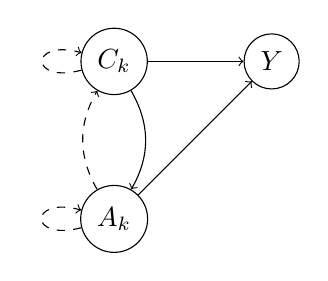
\begin{tikzpicture}%[show background rectangle, scale = 0.5] 
\tikzset{vertex/.style = {shape=circle,draw,minimum size=1.5em}}
\tikzset{edge/.style = {->}}%,> = latex'
% vertices
% \node[vertex,dashed] (U_k) at (3,1) {$U_k$};
% \node[vertex,dashed] (U_k) at (-1,-1) {$U_k$};
\node[vertex] (C_k) at (0,-2) {$C_k$};
% \node[vertex] (C_2) at (2,-2) {$C_2$};
\node[vertex] (A_k) at (0,-4) {$A_k$};
% \node[vertex] (A_2) at (2,-4) {$A_2$};
\node[vertex] (Y) at (2,-2) {$Y$};
% \node[vertex] (A_k) at (1,-3) {$A_k$};
% \node[vertex] (C_k) at (-1,-3) {$C_k$};
% \node[vertex] (Y) at (1,-1) {$Y$};
% \node[vertex] (d) at (4,-3) {$t$};
% \node[vertex] (a1) at (1.5,0) {};
% \node[vertex] (a2) at (3,0) {};
%edges
% \draw[edge,dashed] (U_k) to (C_k);%
% \draw[edge,dashed] (U_k) to (Y);%
% \draw[edge, bend left] (U_k) to (Y);%,dashed
% \draw[edge,bend left] (U_k) to (C_k);%,dashed
% \draw[edge,bend left,red] (C_k) to (U_k);%,dashed
\draw[edge,bend left,dashed] (A_k) to (C_k);
\draw[edge,bend left] (C_k) to (A_k);
\draw[edge] (C_k) to (Y);
\draw[edge] (A_k) to (Y);
% \draw[edge,loop right,directed,red] (U_k) to (U_k);
% \draw[edge,loop left,red] (U_k) to (U_k);%,dashed
\draw[edge,loop left,dashed] (C_k) to (C_k);
\draw[edge,loop left,dashed] (A_k) to (A_k);
% \draw[edge] (X) to[bend left] (Y);
% \draw[edge] (Y) to[bend left] (X);
% \draw[edge] (a) to[bend left] (a1);
% \draw[edge] (a1) to[bend left] (a);
% \draw[edge] (a1) to[bend left] (a2);
% \draw[edge] (a2) to[bend left] (a1);
% \path (a2) to node {\dots} (c);
% \node [shape=circle,minimum size=1.5em] (a3) at (4.5,0) {};
% \draw[edge] (a2) to[bend left] (a3);
% \draw[edge] (a3) to[bend left] (a2);
% \node [shape=circle,minimum size=1.5em] (c1) at (6.5,0) {};
% \draw[edge] (c) to[bend left] (c1);
% \draw[edge] (c1) to[bend left] (c);
\end{tikzpicture} 
}
\end{center}
\caption{Temporal mechanism.}
\label{sfig:nh_mechanism}
}
\end{subfigure}
\hfill
\begin{subfigure}[t]{0.36\textwidth}% \subfigure[After] 
% \subfigure[After] 
{ 
\begin{center}
\resizebox{0.95\textwidth}{!}{
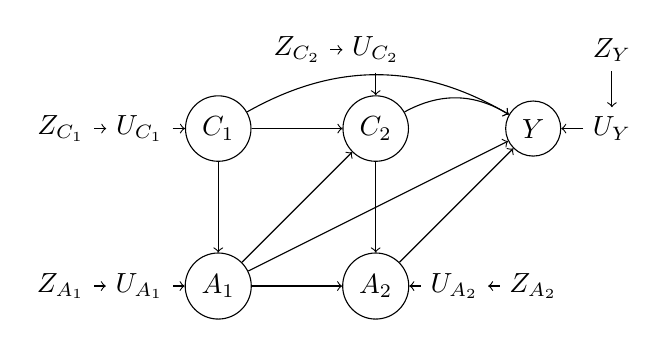
\begin{tikzpicture}%[show background rectangle, scale = 0.5] 
\tikzset{vertex/.style = {shape=circle,draw,minimum size=1.5em}}
\tikzset{edge/.style = {->}}%,> = latex'
% vertices
% \node[vertex,dashed] (U_1) at (0,0) {$U_1$};
% \node[vertex,dashed] (U_2) at (2,0) {$U_2$};
\node[vertex] (C_1) at (0,-2) {$C_1$};
\node[vertex] (C_2) at (2,-2) {$C_2$};
\node[vertex] (A_1) at (0,-4) {$A_1$};
\node[vertex] (A_2) at (2,-4) {$A_2$};
\node[vertex] (Y) at (4,-2) {$Y$};
\node[] (U_C_1) at (-1,-2) {$U_{C_1}$};
\node[] (U_C_2) at (2,-1) {$U_{C_2}$};
\node[] (U_A_1) at (-1,-4) {$U_{A_1}$};
\node[] (U_A_2) at (3,-4) {$U_{A_2}$};
\node[] (U_Y) at (5,-2) {$U_{Y}$};
\node[] (Z_C_1) at (-2,-2) {$Z_{C_1}$};
\node[] (Z_C_2) at (1,-1) {$Z_{C_2}$};
\node[] (Z_A_1) at (-2,-4) {$Z_{A_1}$};
\node[] (Z_A_2) at (4,-4) {$Z_{A_2}$};
\node[] (Z_Y) at (5,-1) {$Z_{Y}$};
% \node[vertex] (d) at (4,-3) {$t$};
% \node[vertex] (a1) at (1.5,0) {};
% \node[vertex] (a2) at (3,0) {};
%edges
\draw[edge] (Z_C_1) to (U_C_1);%
\draw[edge] (Z_C_2) to (U_C_2);%
\draw[edge] (Z_A_1) to (U_A_1);%
\draw[edge] (Z_A_2) to (U_A_2);%
\draw[edge] (Z_Y) to (U_Y);%
\draw[edge] (U_C_1) to (C_1);%
\draw[edge] (U_C_2) to (C_2);%
\draw[edge] (U_A_1) to (A_1);%
\draw[edge] (U_A_2) to (A_2);%
\draw[edge] (U_Y) to (Y);%
\draw[edge, bend left] (C_1) to (Y);
\draw[edge, bend left] (C_2) to (Y);
\draw[edge] (C_1) to (A_1);
\draw[edge] (C_2) to (A_2);
\draw[edge] (A_1) to (Y);
\draw[edge] (A_2) to (Y);
\draw[edge] (A_1) to (C_2);
\draw[edge] (C_1) to (C_2);
\draw[edge] (A_1) to (A_2);
% \draw[edge] (A_2) to (Y);
% \draw[edge] (X) to[bend left] (Y);
% \draw[edge] (Y) to[bend left] (X);
% \draw[edge] (a) to[bend left] (a1);
% \draw[edge] (a1) to[bend left] (a);
% \draw[edge] (a1) to[bend left] (a2);
% \draw[edge] (a2) to[bend left] (a1);
% \path (a2) to node {\dots} (c);
% \node [shape=circle,minimum size=1.5em] (a3) at (4.5,0) {};
% \draw[edge] (a2) to[bend left] (a3);
% \draw[edge] (a3) to[bend left] (a2);
% \node [shape=circle,minimum size=1.5em] (c1) at (6.5,0) {};
% \draw[edge] (c) to[bend left] (c1);
% \draw[edge] (c1) to[bend left] (c);
\end{tikzpicture} 
}
\end{center}
}
% \subfigure%[] 
% % \subfigure[After] 
% { 
% \begin{tikzpicture}%[show background rectangle, scale = 0.5] 
% \tikzset{vertex/.style = {shape=circle,draw,minimum size=1.5em}}
% \tikzset{edge/.style = {->}}%,> = latex'
% % vertices
% % \node[vertex,dashed] (U_1) at (0,0) {$U_1$};
% % \node[vertex,dashed] (U_2) at (2,0) {$U_2$};
% \node[vertex] (C_1) at (0,-2) {$C_1$};
% \node[vertex] (C_2) at (2,-2) {$C_2$};
% \node[vertex, green] (C_3) at (4,-2) {$C_3$};
% \node[vertex] (A_1) at (0,-4) {$A_1$};
% \node[vertex] (A_2) at (2,-4) {$A_2$};
% \node[vertex] (Y) at (6,-2) {$Y$};
% % \node[vertex] (d) at (4,-3) {$t$};
% % \node[vertex] (a1) at (1.5,0) {};
% % \node[vertex] (a2) at (3,0) {};
% %edges
% % \draw[edge,dashed] (U_1) to (C_1);%
% % \draw[edge,dashed] (U_2) to (C_2);%,dashed
% % \draw[edge,dashed] (U_1) to (U_2);%,dashed
% % \draw[edge,dashed] (U_1) to (Y);%,dashed
% % \draw[edge,dashed] (U_2) to (Y);%,dashed
% \draw[edge, bend left] (C_1) to (Y);
% \draw[edge, bend left] (C_2) to (Y);
% \draw[edge, bend left,red] (C_3) to (Y);
% \draw[edge] (C_1) to (A_1);
% \draw[edge] (C_2) to (A_2);
% \draw[edge] (A_1) to (Y);
% \draw[edge] (A_2) to (Y);
% \draw[edge,red] (A_1) to (C_3);
% \draw[edge,red] (A_2) to (C_3);
% \draw[edge, bend left,green] (C_1) to (C_3);
% \draw[edge, bend left,green] (C_2) to (C_3);
% \draw[edge] (A_1) to (C_2);
% \draw[edge] (C_1) to (C_2);
% \draw[edge] (A_1) to (A_2);
% \draw[edge,red] (C_1) to (A_2);
% % \draw[edge] (A_2) to (Y);
% % \draw[edge] (X) to[bend left] (Y);
% % \draw[edge] (Y) to[bend left] (X);
% % \draw[edge] (a) to[bend left] (a1);
% % \draw[edge] (a1) to[bend left] (a);
% % \draw[edge] (a1) to[bend left] (a2);
% % \draw[edge] (a2) to[bend left] (a1);
% % \path (a2) to node {\dots} (c);
% % \node [shape=circle,minimum size=1.5em] (a3) at (4.5,0) {};
% % \draw[edge] (a2) to[bend left] (a3);
% % \draw[edge] (a3) to[bend left] (a2);
% % \node [shape=circle,minimum size=1.5em] (c1) at (6.5,0) {};
% % \draw[edge] (c) to[bend left] (c1);
% % \draw[edge] (c1) to[bend left] (c);
% \end{tikzpicture} 
% \label{sfig:nh_mechanism 2-wave mod}
% }
% }
\caption{$2$-wave model.}
\label{sfig:nh_mechanism 2-wave}
\end{subfigure}
\hfill
\begin{subfigure}[t]{0.45\textwidth}% \subfigure[After] 
{ 
\begin{center}
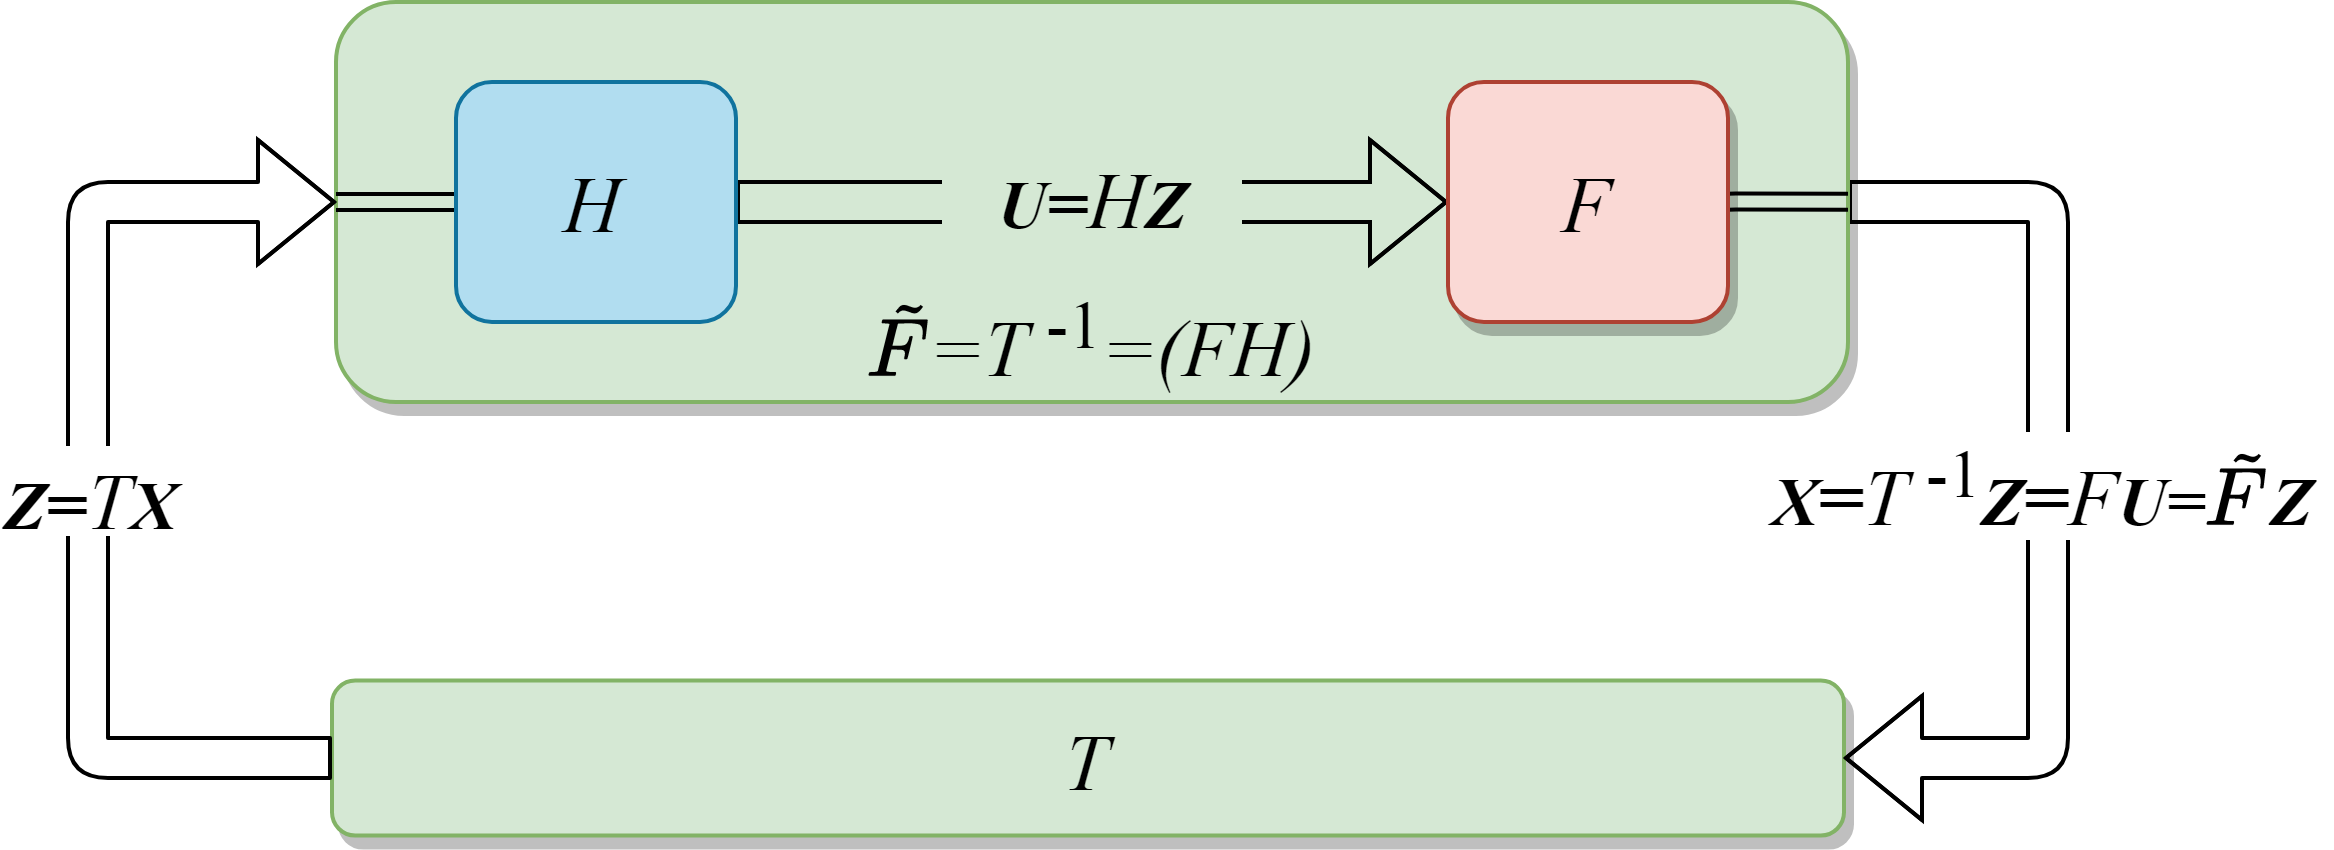
\includegraphics[width=\linewidth,keepaspectratio]{images/c-GNF.png}
\caption{c-GNF architecture for causal and counterfactual inference.}
\label{sfig:c-GNF arch}
\end{center}
}
\end{subfigure}
% \hfill
\caption{Fig.~\ref{sfig:nh_mechanism} shows temporal interactions between the treatments $A_k$ and the observed covariates/confounders $C_k$ at time-wave $k{ = }1,\ldots,K$  and the outcome of interest $Y$. The solid edges indicate the cause and effect at the same time-wave and the dashed edges indicate the one time-wave delayed effect with respect to the respective causes. 
% The dotted lines represent unobservable variables. 
% Note that we make the same critical assumption from~\cite{wodtke2020rwr} that there is no unobserved confounder between $A_k$ and $Y$ unless it is also an unobserved confounding between $C_k$ and $Y$. 
% Observe that (a) is not a Directed Acyclic Graph (DAG) because the variables depend on their past values inducing a cycle/loop. However, we can modify (a) into the DAGs shown in (b) and (c) by unwinding the general mechanism in time. %Fig. \ref{sfig:nh_mechanism},
Fig.~\ref{sfig:nh_mechanism 2-wave} represents the 2-wave model of Fig.~\ref{sfig:nh_mechanism}.
% Fig.~\ref{sfig:nh_mechanism}, Figs.~\ref{sfig:nh_mechanism 1-wave}, \ref{sfig:nh_mechanism 2-wave}
For any given observed endogenous variable $X$ in Fig.~\ref{sfig:nh_mechanism 2-wave}, $U_X$ and $Z_X$ respectively denote the unobserved exogenous noises of the true SCM $F{ : }\mathbf{U}{ \rightarrow }\mathbf{X}$ and the \emph{encapsulated-SCM} $\tilde{F}{ = }(FH){ = }T^{-1}{ : }\mathbf{Z}{ \rightarrow }\mathbf{X}$ in Fig.~\ref{sfig:c-GNF arch}, where $H{ : }\mathbf{Z}{ \rightarrow }\mathbf{U}$ denotes an auxiliary transformation. Since $\tilde{F}$ (green) encapsulates $F$ (red) and $H$ (blue) SCMs, i.e., $\tilde{F}{ = }(FH){ = }T^{-1}$, we refer to $\tilde{F}$ as the \emph{encapsulated-SCM}.
Our c-GNF models $T{ : }\mathbf{X}{ \rightarrow }\mathbf{Z}$ and readily provides the \emph{encapsulated-SCM} $\tilde{F}{ : }\mathbf{Z}{ \rightarrow }\mathbf{X}$, as $T$ is invertible by construction, facilitating counterfactual inference using \emph{`The First Law of Causal Inference'}~\cite{pearl2009abductionactionprediction, pearl2009causality}.
% Fig.~\ref{sfig:c-GNF arch} represents the 
% As examples we show the 2-wave model and the 3-wave model in (b) and (c) respectively.%~\ref{sfig:nh_mechanism 2-wave} and ~\ref{sfig:nh_mechanism 3-wave}.
}
\label{fig:nh_causaC_model all}
\end{figure*}
% Personalizing Public Policies In Social Science Using Causal-Graphical Normalizing Flows
%It is very well known that correlation does not imply causation~\cite{wright1921correlationcausation} and the fields of critical social impact such as economics, epidemiology and social science have been exploring various ways to identify and estimate the causal effects.
%Since 1970s, Structural Equation Models (SEMs), developed from Wright's path analysis~\cite{wright1921correlationcausation}, have been very widely used in economics~\cite{Haavelmo1943SEM, Goldberger1972SEMecon} and social sciences~\cite{Duncan1974SEMsocio, Ploch1975SEM, Fienberg1975Introduction2SEM} to understand and perform causal inference that had demonstrated tremendous success in terms of practical social impact. However, due to the complex nature of identifying SEM parameters, since 1980s, Inverse Probability Weighting (IPW)~\cite{Rosenbaum1983propensityscoreipw, hernan2009ipw} predominantly popular in fields such as epidemiology, sociology, political science, provides a simple and effect way to estimate average treatment effects without the need to model the entire causal mechanism by using Importance Sampling technique to evaluate expectation of potential outcomes from the target interventional distribution using the observational distributions as the proposal distribution. % ~\cite{horvitz1952generalization}
% As a results, IPW has been very popular in economics and social science since. Even though, deep learning has been recently demonstrated to be extremely successful in the fields of computer science such as computer vision, speech processing, natural language processing, autonomous driving, robotics, etc. very little adaptation has been seen in fields such as epidemiology, sociology, political science, etc. that mainly focus on causality, particularly the field of social science research that has severe social impact.
% Propensity weighting methods such as IPW, IPW trimming, Overlap Weighting (OW)~\cite{fan2018overlapweightsipw} have been very well studied and widely used in the field of epidemiology, economics, sociology etc. to provide the unbiased estimates of causal effects under certain assumptions of the correct functional forms. 
%The prominent real-world social science work~\cite{wodtke2011ipw} studies the longitudinal long-term time-varying neighborhood effects on the high-school graduation using stabilised IPW.
%Even though the findings of neighborhood effects on the high-school graduation are quite fascinating, consistent with other real-world causal estimation problems, the causal effect estimates cannot be verified with the unknown true causal effect. %obtained from IPW is not verifiable as the true causal effects are unknown for validating the estimate.
%As a result, in a more recent work comparison to~\cite{wodtke2011ipw},~\citeauthor{wodtke2020rwr} proposes Regression-with-Residual (RWR)~\cite{wodtke2020rwr} as a competing alternative to IPW with lesser variance in the causal effect estimates under the assumption that the functional forms of the outcome model is correctly specified. However due to the use of a single outcome model similar to S(Single)-Learner~\cite{kunzel2019metalearners}, RWR provides biased estimates 
%under effect modification/heterogeneity in the data. 
% Apart from IPW and RWR, we also explore an alternate graphical approach of directly modeling the desired outcome using regression models/metalearners~\cite{kunzel2019metalearners} (S-Learner, T-Learner, X-Learner, etc) as a function of the time-varying treatments and covariates using the expression identified from the rules of $do$-calculus.
% It is interesting to observe that the $G$-computation formula~\cite{ROBINS1986gcom, hernan2009ipw, pearl2009causality} is equivalent to the causal effect estimation expression identified by the $do$-calculus. 
% Hence we refer to the model designed using the $do$-calculus expression as Grouped Conditional Outcome Model (GCOM) even though it can often be referred with other names such as G-computation estimators, parametric G-formula, or standardization in epidemiology and biostatistics.
%To address effect modification/heterogeneity in data, a class of Meta-Learners~\cite{kunzel2019metalearners} such T(Two)-Learner, X-Learner, etc~\cite{kunzel2019metalearners}, have been proposed where separate conditional outcome regression models are trained individually for each treatment group, we refer to this as Grouped Conditional Outcome Model (GCOM).
% depending on the number of conditional outcome models used, the metalearners are mainly classified as S-Learner, T-Learner, X-Learner, etc~\cite{kunzel2019metalearners}. 
% The expression used for the outcome regression models is based on $G$-computation formula ($g$-estimation) 
%The non-parametric expression of the conditional outcome regression model can be obtained from $do$-calculus~\cite{pearl2009causality, pearl2012docalculus} or $G$-computation formula ($g$-estimation)~\cite{ROBINS1986gcom, hernan2009ipw, pearl2009causality} by adjusting for confounding.
%Compared to $G$-computation formula, $do$-calculus provides a more complete identification of the causal estimands in terms the statistical estimands that can be modeled using statistical models.
% and also the models are nothing but conditional regression models trained individually on each treatment group, we refer to this as Grouped Conditional Outcome Model (GCOM).
%As stated previously, if IPW solely requires right propensity score model, RWR/GCOM methods solely require the right outcome model. However, Doubly Robust (DR) methods~\cite{bang2005doublyrobust} are a class of causal effect estimation methods that model both propensity score and outcome but are robust in the sense that they only require either one of the treatment or the outcome model to be right to provide unbiased estimates of Average Causal Effect (ACE).
% A common limitation/assumption of propensity score weighting methods such as IPW, OW and etc is the availability of an ideal propensity score model for calculating the inverse propensity weights, i.e., the exact functional forms of the propensity score model is known. Since the weights are calculated directly as inverse of propensity scores, it is a given core assumption that the propensity score model to be perfect to result in unbiased causal effect estimates. The effect of propensity score model misspecification on IPW has been studied in~\cite{zhou2020propensityipw}. The effect of the violation of the exact propensity score model specification assumption in weighting methods has been studied in~\cite{williamson2014varianceipw, austin2015bestpracticeipw, zhou2020propensityipw}.

%In contrast to the above well established causal effect estimation methods such as IPW/RWR/GCOM/DR that require correct functional form assumptions for their model, in this work, we adopt the deep learning approach Graphical Normalizing Flow (GNF) for causal inference, which we refer to as causal-GNF (c-GNF) without the need of the right functional form specification of treatment and/or outcome model. 
%Even though we predominantly consider the social science work of neighborhood effects with time-varying treatments and time-varying confounders~\cite{wodtke2020rwr} in this work (Fig.~\ref{sfig:nh_mechanism 2-wave}), our work in causal inference is not just limited to social science but is equally applicable to several other fields such as epidemiology, economics, political science, biostatistics, etc that have a significant social impact.
%We list the following contributions of our work applicable to  below.

Since the realization that correlation does not imply causation~\cite{wright1921correlationcausation, fisher1936designofexperiments}, statisticians, computer scientists, and social scientists have been developing ways to identify and estimate causal effects from observational data.
By the 1970s, Structural Equation Models (SEMs), developed from Wright's path analysis~\cite{wright1921correlationcausation} in genetics, have been widely used in economics~\cite{Haavelmo1943SEM, Goldberger1972SEMecon} and other social sciences~\cite{Duncan1974SEMsocio, Ploch1975SEM, Fienberg1975Introduction2SEM} to analyze cause and effect. 
Pearl's Structural Causal Model (SCM)~\cite{pearl2009causality} provides an explicit causal definition to disambiguate the causes and effects by replacing the symmetric `=' operator with asymmetric `:=' assignment operator, thereby complementing the original SEM definition.
Energized by this and similar developments in computer science, a causal revolution has occurred with large ramifications not only in academia but also for how governments, non-governmental organizations, and international organizations (such as the World Bank, United Nations Childrens Fund (UNICEF), or International Monetary Fund) articulate public policies to combat social ills. For example, to combat poverty, governments use mainly an individual's income and similar characteristics to identify vulnerable population and then assess if they are eligible for social welfare eligibility. Then a simple rule is often applied: if they are eligible, they tend to receive a fixed one-size-fits-all public policy; if they are not eligible, no policy is ascribed. Although such public-policy making is highly transparent as it applies what is best on average for a population -- that is the average causal effect (ACE) -- it lacks an adaptability necessary to efficiently combat poverty, ill-health, and other social ills. For effective combating, government officials and others require methods that are able to personalize these policies~\cite{kino2021adelmlreview}. That is, personalized public policy analysis (P$^3$A) requires methods that can move beyond ACE estimation, and into counterfactual inference.
% \footnote{JMP: For the acronym SEM, you capitalize the first letters of each word when you introduce the acronym: Structural Equation Model (SEM). However, you don't do the same when you introduce ACE, CACE, P3A. When you have several references, they are typically sorted alphabetically, e.g. the ordering in (Haavelmo 1943, Goldberger 1972) should be reversed.\newline SB:These things were modified by Adel. I always capitalize the definitions and abbreviations. The IPW/RWR was reedited by Adel!? Please refer to my original draft. That's why I asked to comment my part when adding new content and not delete it so that it's easy for me to know what part is edited!! Ordering of grouped citations I have done according to the chronological order. First work gets first citation and so on. It was just my writing choice that I decided when I started writing the paper from scratch.}

However, traditional statistical causal effect estimation methods, such as Inverse Probability Weighting (IPW)~\cite{Rosenbaum1983propensityscoreipw, hernan2009ipw} or recent ones such as Regression-With-Residuals (RWR)~\cite{wodtke2020rwr}, focus on ACE estimation only. An advantage of IPW (stabilized) is that it provides a simple and effective way to estimate ACE without the need to model the entire causal system, under the assumption that the functional form of the propensity score is correctly specified. In contrast to IPW, RWR, which comes under the class of outcome regression models, estimate ACEs more effectively (less variance), under the assumption that the functional form of the outcome models are correctly specified. 
However due to the use of a single outcome model similar to S(Single)-Learner, RWR provides biased estimates when there is effect modification in data (also know as effect heterogeneity)~\cite{vanderweele2009distinctionheterogeneity}.  
% \begin{figure*}[ht!]
% \begin{subfigure}[t]{0.18\textwidth}% \subfigure[After] 
% { 
% \begin{center}
% \resizebox{0.85\textwidth}{!}{
% \begin{tikzpicture}%[show background rectangle, scale = 0.5] 
% \tikzset{vertex/.style = {shape=circle,draw,minimum size=1.5em}}
% \tikzset{edge/.style = {->}}%,> = latex'
% % vertices
% % \node[vertex,dashed] (U_k) at (3,1) {$U_k$};
% % \node[vertex,dashed] (U_k) at (-1,-1) {$U_k$};
% \node[vertex] (C_k) at (0,-2) {$C_k$};
% % \node[vertex] (C_2) at (2,-2) {$C_2$};
% \node[vertex] (A_k) at (0,-4) {$A_k$};
% % \node[vertex] (A_2) at (2,-4) {$A_2$};
% \node[vertex] (Y) at (2,-2) {$Y$};
% % \node[vertex] (A_k) at (1,-3) {$A_k$};
% % \node[vertex] (C_k) at (-1,-3) {$C_k$};
% % \node[vertex] (Y) at (1,-1) {$Y$};
% % \node[vertex] (d) at (4,-3) {$t$};
% % \node[vertex] (a1) at (1.5,0) {};
% % \node[vertex] (a2) at (3,0) {};
% %edges
% % \draw[edge,dashed] (U_k) to (C_k);%
% % \draw[edge,dashed] (U_k) to (Y);%
% % \draw[edge, bend left] (U_k) to (Y);%,dashed
% % \draw[edge,bend left] (U_k) to (C_k);%,dashed
% % \draw[edge,bend left,red] (C_k) to (U_k);%,dashed
% \draw[edge,bend left,dashed] (A_k) to (C_k);
% \draw[edge,bend left] (C_k) to (A_k);
% \draw[edge] (C_k) to (Y);
% \draw[edge] (A_k) to (Y);
% % \draw[edge,loop right,directed,red] (U_k) to (U_k);
% % \draw[edge,loop left,red] (U_k) to (U_k);%,dashed
% \draw[edge,loop left,dashed] (C_k) to (C_k);
% \draw[edge,loop left,dashed] (A_k) to (A_k);
% % \draw[edge] (X) to[bend left] (Y);
% % \draw[edge] (Y) to[bend left] (X);
% % \draw[edge] (a) to[bend left] (a1);
% % \draw[edge] (a1) to[bend left] (a);
% % \draw[edge] (a1) to[bend left] (a2);
% % \draw[edge] (a2) to[bend left] (a1);
% % \path (a2) to node {\dots} (c);
% % \node [shape=circle,minimum size=1.5em] (a3) at (4.5,0) {};
% % \draw[edge] (a2) to[bend left] (a3);
% % \draw[edge] (a3) to[bend left] (a2);
% % \node [shape=circle,minimum size=1.5em] (c1) at (6.5,0) {};
% % \draw[edge] (c) to[bend left] (c1);
% % \draw[edge] (c1) to[bend left] (c);
% \end{tikzpicture} 
% }
% \end{center}
% \caption{Temporal mechanism.}
% \label{sfig:nh_mechanism}
% }
% \end{subfigure}
% \hfill
% \begin{subfigure}[t]{0.36\textwidth}% \subfigure[After] 
% % \subfigure[After] 
% { 
% \begin{center}
% \resizebox{0.95\textwidth}{!}{
% \begin{tikzpicture}%[show background rectangle, scale = 0.5] 
% \tikzset{vertex/.style = {shape=circle,draw,minimum size=1.5em}}
% \tikzset{edge/.style = {->}}%,> = latex'
% % vertices
% % \node[vertex,dashed] (U_1) at (0,0) {$U_1$};
% % \node[vertex,dashed] (U_2) at (2,0) {$U_2$};
% \node[vertex] (C_1) at (0,-2) {$C_1$};
% \node[vertex] (C_2) at (2,-2) {$C_2$};
% \node[vertex] (A_1) at (0,-4) {$A_1$};
% \node[vertex] (A_2) at (2,-4) {$A_2$};
% \node[vertex] (Y) at (4,-2) {$Y$};
% \node[] (U_C_1) at (-1,-2) {$U_{C_1}$};
% \node[] (U_C_2) at (2,-1) {$U_{C_2}$};
% \node[] (U_A_1) at (-1,-4) {$U_{A_1}$};
% \node[] (U_A_2) at (3,-4) {$U_{A_2}$};
% \node[] (U_Y) at (5,-2) {$U_{Y}$};
% \node[] (Z_C_1) at (-2,-2) {$Z_{C_1}$};
% \node[] (Z_C_2) at (1,-1) {$Z_{C_2}$};
% \node[] (Z_A_1) at (-2,-4) {$Z_{A_1}$};
% \node[] (Z_A_2) at (4,-4) {$Z_{A_2}$};
% \node[] (Z_Y) at (5,-1) {$Z_{Y}$};
% % \node[vertex] (d) at (4,-3) {$t$};
% % \node[vertex] (a1) at (1.5,0) {};
% % \node[vertex] (a2) at (3,0) {};
% %edges
% \draw[edge] (Z_C_1) to (U_C_1);%
% \draw[edge] (Z_C_2) to (U_C_2);%
% \draw[edge] (Z_A_1) to (U_A_1);%
% \draw[edge] (Z_A_2) to (U_A_2);%
% \draw[edge] (Z_Y) to (U_Y);%
% \draw[edge] (U_C_1) to (C_1);%
% \draw[edge] (U_C_2) to (C_2);%
% \draw[edge] (U_A_1) to (A_1);%
% \draw[edge] (U_A_2) to (A_2);%
% \draw[edge] (U_Y) to (Y);%
% \draw[edge, bend left] (C_1) to (Y);
% \draw[edge, bend left] (C_2) to (Y);
% \draw[edge] (C_1) to (A_1);
% \draw[edge] (C_2) to (A_2);
% \draw[edge] (A_1) to (Y);
% \draw[edge] (A_2) to (Y);
% \draw[edge] (A_1) to (C_2);
% \draw[edge] (C_1) to (C_2);
% \draw[edge] (A_1) to (A_2);
% % \draw[edge] (A_2) to (Y);
% % \draw[edge] (X) to[bend left] (Y);
% % \draw[edge] (Y) to[bend left] (X);
% % \draw[edge] (a) to[bend left] (a1);
% % \draw[edge] (a1) to[bend left] (a);
% % \draw[edge] (a1) to[bend left] (a2);
% % \draw[edge] (a2) to[bend left] (a1);
% % \path (a2) to node {\dots} (c);
% % \node [shape=circle,minimum size=1.5em] (a3) at (4.5,0) {};
% % \draw[edge] (a2) to[bend left] (a3);
% % \draw[edge] (a3) to[bend left] (a2);
% % \node [shape=circle,minimum size=1.5em] (c1) at (6.5,0) {};
% % \draw[edge] (c) to[bend left] (c1);
% % \draw[edge] (c1) to[bend left] (c);
% \end{tikzpicture} 
% }
% \end{center}
% }
% % \subfigure%[] 
% % % \subfigure[After] 
% % { 
% % \begin{tikzpicture}%[show background rectangle, scale = 0.5] 
% % \tikzset{vertex/.style = {shape=circle,draw,minimum size=1.5em}}
% % \tikzset{edge/.style = {->}}%,> = latex'
% % % vertices
% % % \node[vertex,dashed] (U_1) at (0,0) {$U_1$};
% % % \node[vertex,dashed] (U_2) at (2,0) {$U_2$};
% % \node[vertex] (C_1) at (0,-2) {$C_1$};
% % \node[vertex] (C_2) at (2,-2) {$C_2$};
% % \node[vertex, green] (C_3) at (4,-2) {$C_3$};
% % \node[vertex] (A_1) at (0,-4) {$A_1$};
% % \node[vertex] (A_2) at (2,-4) {$A_2$};
% % \node[vertex] (Y) at (6,-2) {$Y$};
% % % \node[vertex] (d) at (4,-3) {$t$};
% % % \node[vertex] (a1) at (1.5,0) {};
% % % \node[vertex] (a2) at (3,0) {};
% % %edges
% % % \draw[edge,dashed] (U_1) to (C_1);%
% % % \draw[edge,dashed] (U_2) to (C_2);%,dashed
% % % \draw[edge,dashed] (U_1) to (U_2);%,dashed
% % % \draw[edge,dashed] (U_1) to (Y);%,dashed
% % % \draw[edge,dashed] (U_2) to (Y);%,dashed
% % \draw[edge, bend left] (C_1) to (Y);
% % \draw[edge, bend left] (C_2) to (Y);
% % \draw[edge, bend left,red] (C_3) to (Y);
% % \draw[edge] (C_1) to (A_1);
% % \draw[edge] (C_2) to (A_2);
% % \draw[edge] (A_1) to (Y);
% % \draw[edge] (A_2) to (Y);
% % \draw[edge,red] (A_1) to (C_3);
% % \draw[edge,red] (A_2) to (C_3);
% % \draw[edge, bend left,green] (C_1) to (C_3);
% % \draw[edge, bend left,green] (C_2) to (C_3);
% % \draw[edge] (A_1) to (C_2);
% % \draw[edge] (C_1) to (C_2);
% % \draw[edge] (A_1) to (A_2);
% % \draw[edge,red] (C_1) to (A_2);
% % % \draw[edge] (A_2) to (Y);
% % % \draw[edge] (X) to[bend left] (Y);
% % % \draw[edge] (Y) to[bend left] (X);
% % % \draw[edge] (a) to[bend left] (a1);
% % % \draw[edge] (a1) to[bend left] (a);
% % % \draw[edge] (a1) to[bend left] (a2);
% % % \draw[edge] (a2) to[bend left] (a1);
% % % \path (a2) to node {\dots} (c);
% % % \node [shape=circle,minimum size=1.5em] (a3) at (4.5,0) {};
% % % \draw[edge] (a2) to[bend left] (a3);
% % % \draw[edge] (a3) to[bend left] (a2);
% % % \node [shape=circle,minimum size=1.5em] (c1) at (6.5,0) {};
% % % \draw[edge] (c) to[bend left] (c1);
% % % \draw[edge] (c1) to[bend left] (c);
% % \end{tikzpicture} 
% % \label{sfig:nh_mechanism 2-wave mod}
% % }
% % }
% \caption{$2$-wave model.}
% \label{sfig:nh_mechanism 2-wave}
% \end{subfigure}
% \hfill
% \begin{subfigure}[t]{0.45\textwidth}% \subfigure[After] 
% { 
% \begin{center}
% 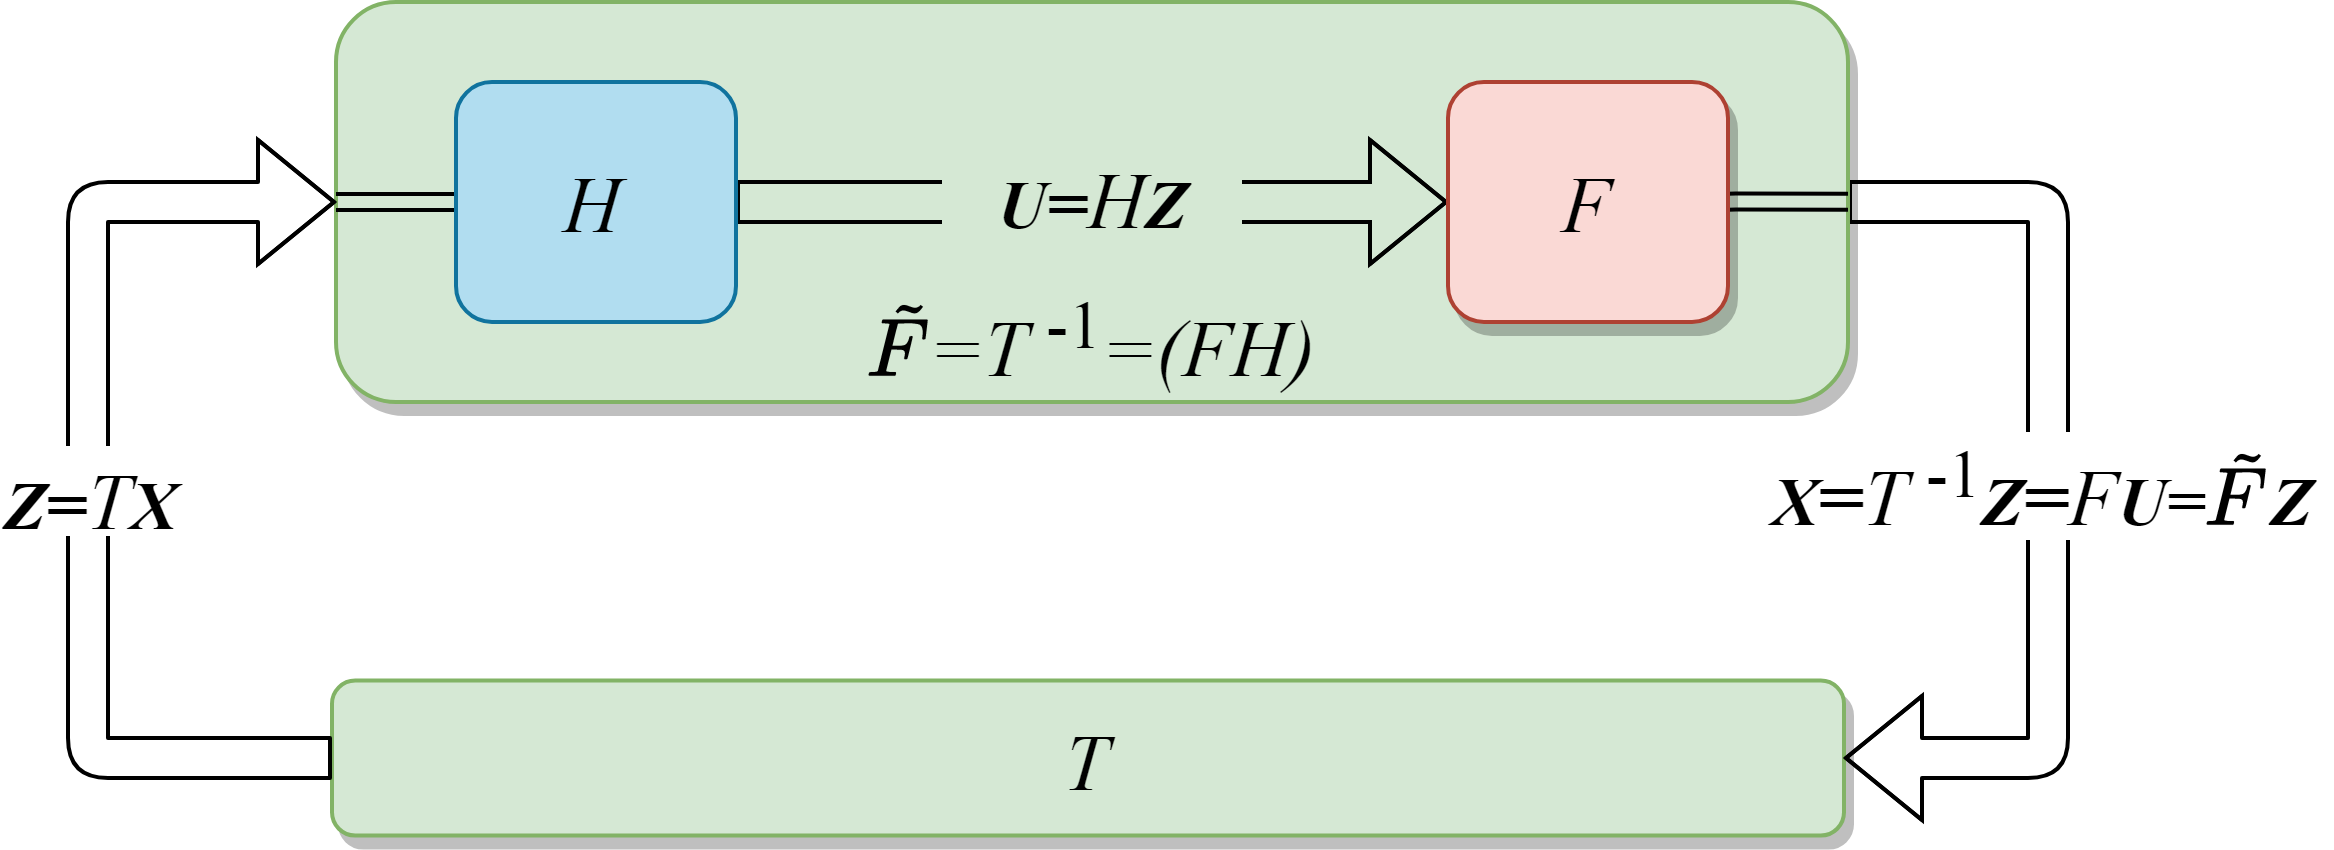
\includegraphics[width=\linewidth,keepaspectratio]{images/c-GNF.png}
% \caption{c-GNF architecture.}
% \label{sfig:c-GNF arch}
% \end{center}
% }
% \end{subfigure}
% % \hfill
% \caption{Fig.~\ref{sfig:nh_mechanism} shows temporal interactions between the treatments $A_k$ and the observed covariates/confounders $C_k$ at time-wave $k{ = }1,\ldots,K$  and the outcome of interest $Y$. The solid edges indicate the cause and effect at the same time-wave and the dashed edges indicate the one time-wave delayed effect with respect to the respective causes. 
% % The dotted lines represent unobservable variables. 
% % Note that we make the same critical assumption from~\cite{wodtke2020rwr} that there is no unobserved confounder between $A_k$ and $Y$ unless it is also an unobserved confounding between $C_k$ and $Y$. 
% % Observe that (a) is not a Directed Acyclic Graph (DAG) because the variables depend on their past values inducing a cycle/loop. However, we can modify (a) into the DAGs shown in (b) and (c) by unwinding the general mechanism in time. %Fig. \ref{sfig:nh_mechanism},
% Fig.~\ref{sfig:nh_mechanism 2-wave} represents the 2-wave model of Fig.~\ref{sfig:nh_mechanism}.
% % Fig.~\ref{sfig:nh_mechanism}, Figs.~\ref{sfig:nh_mechanism 1-wave}, \ref{sfig:nh_mechanism 2-wave}
% For a given observed endogenous variable $X$ in Fig.~\ref{sfig:nh_mechanism 2-wave}, $U_X$ and $Z_X$ respectively denote the unobserved exogenous noises of the true SCM $F{ : }\mathbf{U}{ \rightarrow }\mathbf{X}$ and the \emph{encapsulated-SCM} $\tilde{F}{ : }\mathbf{Z}{ \rightarrow }\mathbf{X}$ in Fig.~\ref{sfig:c-GNF arch}, where $H{ : }\mathbf{Z}{ \rightarrow }\mathbf{U}$ denotes an auxiliary transformation. Since $\tilde{F} ({ = }T^{-1})$ (green) encapsulates $F$ (red) and $H$ (blue) SCMs, i.e., $\tilde{F}{ = }(FH){ = }T^{-1}$, we refer to $\tilde{F}$ as the \emph{encapsulated-SCM}.
% Our proposed c-GNF models $T$ and readily provides the inverse $T^{-1}$, i.e., \emph{encapsulated-SCM} $\tilde{F}$, by construction, facilitating counterfactual inference using \emph{`The First Law of Causal Inference'}~\cite{pearl2009abductionactionprediction, pearl2009causality}.
% % Fig.~\ref{sfig:c-GNF arch} represents the 
% % As examples we show the 2-wave model and the 3-wave model in (b) and (c) respectively.%~\ref{sfig:nh_mechanism 2-wave} and ~\ref{sfig:nh_mechanism 3-wave}.
% }
% \label{fig:nh_causaC_model all}
% \end{figure*}

To directly address effect modification, computer scientists have developed a class of outcome regression based machine-learning models called meta-learners~\cite{kunzel2019metalearners} (e.g., T(Two)-Learner, X-Learner) where each treatment group is modeled using a separate outcome regression models conditioned on proper adjustment sets to account for any confounding.
Since meta-learners model separate conditional outcome regression models for each treatment groups, we alternatively refer them as Grouped Conditional Outcome Model (GCOM).
% , i.e., Outcome Model which is Conditional on the adjustment set and Grouped by treatment groups. 
The conditioning set or adjustment set or the predictors of outcome regression model are identified from the non-parametric expression of the interventional distribution obtained from $do$-calculus~\cite{pearl2009causality, pearl2012docalculus} or $G$-computation formula~\cite{ROBINS1986gcom, hernan2009ipw} to accurately model and estimate the causal effects of interest by adjusting for the confounding.
% The non-parametric expression of the conditional outcome regression model can be obtained from $do$-calculus~\cite{pearl2009causality} or $g$-estimation~\cite{ROBINS1986gcom, hernan2009ipw} by adjusting for confounding, i.e., the non-parametric expression provides the right adjustment set to account for in the outcome regression modeling to be able to accurately estimate the causal effects of interest. 
While IPW requires the right propensity score model, RWR and GCOM methods require the correct outcome model. 
% To incorporate the best of these two approaches, 
In contrast, Doubly Robust (DR)~\cite{bang2005doublyrobust} methods are a class of causal inference methods that incorporate the best of IPW and GCOM by jointly modeling the propensity score and the outcome. The key advantage of DR is that it requires only either one of the propensity or the outcome model to be  correctly specified to produce unbiased ACE estimates. Notwithstanding the advantages of IPW, RWR, GCOM, and DR, none of them successfully supply a method to conduct counterfactual inference for P$^3$A. 

In this work, we aim to further P$^3$A and causal inference in the social science by demonstrating a method for counterfactual inference that does not require a priori knowledge of the correct functional form in neither the propensity score or the outcome model. Our causal method consists of a flow-based deep learning approach known as Graphical Normalizing Flows (GNFs). As we re-purpose GNFs for causal inference by using causal-Directed Acyclic Graphs (causal-DAGs), we refer them as causal-GNFs (c-GNFs). Even though we focus on the social effect of neighborhood on children's education outcomes~\cite{wodtke2020rwr} as an example of P$^3$A in this article, our contributions are applicable to other settings in epidemiology, economics, sociology, and political science, where counterfactual policy-making is critical to promote social, material, and health outcomes. 
Our work supplies at least the following five contributions.
% \begin{figure}[t!]
%     % \centering
% % \begin{subfigure}[t]{0.23\textwidth}
% % % \subfigure[After] 
% % { 
% % \begin{tikzpicture}%[show background rectangle, scale = 0.5] 
% % \tikzset{vertex/.style = {shape=circle,draw,minimum size=1.5em}}
% % \tikzset{edge/.style = {->}}%,> = latex'
% % % vertices
% % % \node[vertex,dashed] (U_k) at (3,1) {$U_k$};
% % \node[vertex,dashed] (U_k) at (-1,-1) {$U_k$};
% % \node[vertex] (A_k) at (-1,-3) {$A_k$};
% % \node[vertex] (Y) at (1,-1) {$Y$};
% % % \node[vertex] (d) at (4,-3) {$t$};
% % % \node[vertex] (a1) at (1.5,0) {};
% % % \node[vertex] (a2) at (3,0) {};
% % %edges
% % % \draw[edge,dashed] (U_k) to (C_k);%
% % % \draw[edge,dashed] (U_k) to (Y);%
% % \draw[edge, bend left,dashed] (U_k) to (Y);
% % \draw[edge,bend left,dashed] (U_k) to (A_k);
% % \draw[edge,bend left,directed,red,dashed] (A_k) to (U_k);
% % \draw[edge] (A_k) to (Y);
% % % \draw[edge,loop right,directed,red] (U_k) to (U_k);
% % \draw[edge,loop left,directed,red,dashed] (U_k) to (U_k);
% % \draw[edge,loop left,directed,red,dashed] (A_k) to (A_k);
% % % \draw[edge] (X) to[bend left] (Y);
% % % \draw[edge] (Y) to[bend left] (X);
% % % \draw[edge] (a) to[bend left] (a1);
% % % \draw[edge] (a1) to[bend left] (a);
% % % \draw[edge] (a1) to[bend left] (a2);
% % % \draw[edge] (a2) to[bend left] (a1);
% % % \path (a2) to node {\dots} (c);
% % % \node [shape=circle,minimum size=1.5em] (a3) at (4.5,0) {};
% % % \draw[edge] (a2) to[bend left] (a3);
% % % \draw[edge] (a3) to[bend left] (a2);
% % % \node [shape=circle,minimum size=1.5em] (c1) at (6.5,0) {};
% % % \draw[edge] (c) to[bend left] (c1);
% % % \draw[edge] (c1) to[bend left] (c);
% % \end{tikzpicture} 
% % \label{sfig:nh_mechanism confounder}
% % }
% % \caption{}
% % \end{subfigure}
% % \hfill
% % \begin{subfigure}[t]{0.24\textwidth}% \subfigure[After] 
% % { 
% % \begin{center}
% % \begin{tikzpicture}%[show background rectangle, scale = 0.5] 
% % \tikzset{vertex/.style = {shape=circle,draw,minimum size=1.5em}}
% % \tikzset{edge/.style = {->}}%,> = latex'
% % % vertices
% % % \node[vertex,dashed] (U_k) at (3,1) {$U_k$};
% % \node[vertex,dashed] (U_k) at (-1,-1) {$U_k$};
% % \node[vertex] (A_k) at (1,-3) {$A_k$};
% % \node[vertex] (C_k) at (-1,-3) {$C_k$};
% % \node[vertex] (Y) at (1,-1) {$Y$};
% % % \node[vertex] (d) at (4,-3) {$t$};
% % % \node[vertex] (a1) at (1.5,0) {};
% % % \node[vertex] (a2) at (3,0) {};
% % %edges
% % % \draw[edge,dashed] (U_k) to (C_k);%
% % % \draw[edge,dashed] (U_k) to (Y);%
% % \draw[edge, bend left] (U_k) to (Y);%,dashed
% % \draw[edge,bend left] (U_k) to (C_k);%,dashed
% % \draw[edge,bend left,red] (C_k) to (U_k);%,dashed
% % \draw[edge,bend left,red] (A_k) to (C_k);
% % \draw[edge,bend left] (C_k) to (A_k);
% % \draw[edge] (C_k) to (Y);
% % \draw[edge] (A_k) to (Y);
% % % \draw[edge,loop right,directed,red] (U_k) to (U_k);
% % \draw[edge,loop left,red] (U_k) to (U_k);%,dashed
% % \draw[edge,loop left,red] (C_k) to (C_k);
% % \draw[edge,loop right,red] (A_k) to (A_k);
% % % \draw[edge] (X) to[bend left] (Y);
% % % \draw[edge] (Y) to[bend left] (X);
% % % \draw[edge] (a) to[bend left] (a1);
% % % \draw[edge] (a1) to[bend left] (a);
% % % \draw[edge] (a1) to[bend left] (a2);
% % % \draw[edge] (a2) to[bend left] (a1);
% % % \path (a2) to node {\dots} (c);
% % % \node [shape=circle,minimum size=1.5em] (a3) at (4.5,0) {};
% % % \draw[edge] (a2) to[bend left] (a3);
% % % \draw[edge] (a3) to[bend left] (a2);
% % % \node [shape=circle,minimum size=1.5em] (c1) at (6.5,0) {};
% % % \draw[edge] (c) to[bend left] (c1);
% % % \draw[edge] (c1) to[bend left] (c);
% % \end{tikzpicture} 
% % \caption{General temporal mechanism.}
% % \label{sfig:nh_mechanism}
% % \end{center}
% % }
% % \end{subfigure}
% \begin{subfigure}[t]{0.24\textwidth}% \subfigure[After] 
% { 
% \begin{center}
% \begin{tikzpicture}%[show background rectangle, scale = 0.5] 
% \tikzset{vertex/.style = {shape=circle,draw,minimum size=1.5em}}
% \tikzset{edge/.style = {->}}%,> = latex'
% % vertices
% % \node[vertex,dashed] (U_k) at (3,1) {$U_k$};
% % \node[vertex,dashed] (U_k) at (-1,-1) {$U_k$};
% \node[vertex] (C_k) at (0,-2) {$C_k$};
% % \node[vertex] (C_2) at (2,-2) {$C_2$};
% \node[vertex] (A_k) at (0,-4) {$A_k$};
% % \node[vertex] (A_2) at (2,-4) {$A_2$};
% \node[vertex] (Y) at (2,-2) {$Y$};
% % \node[vertex] (A_k) at (1,-3) {$A_k$};
% % \node[vertex] (C_k) at (-1,-3) {$C_k$};
% % \node[vertex] (Y) at (1,-1) {$Y$};
% % \node[vertex] (d) at (4,-3) {$t$};
% % \node[vertex] (a1) at (1.5,0) {};
% % \node[vertex] (a2) at (3,0) {};
% %edges
% % \draw[edge,dashed] (U_k) to (C_k);%
% % \draw[edge,dashed] (U_k) to (Y);%
% % \draw[edge, bend left] (U_k) to (Y);%,dashed
% % \draw[edge,bend left] (U_k) to (C_k);%,dashed
% % \draw[edge,bend left,red] (C_k) to (U_k);%,dashed
% \draw[edge,bend left,dashed] (A_k) to (C_k);
% \draw[edge,bend left] (C_k) to (A_k);
% \draw[edge] (C_k) to (Y);
% \draw[edge] (A_k) to (Y);
% % \draw[edge,loop right,directed,red] (U_k) to (U_k);
% % \draw[edge,loop left,red] (U_k) to (U_k);%,dashed
% \draw[edge,loop left,dashed] (C_k) to (C_k);
% \draw[edge,loop left,dashed] (A_k) to (A_k);
% % \draw[edge] (X) to[bend left] (Y);
% % \draw[edge] (Y) to[bend left] (X);
% % \draw[edge] (a) to[bend left] (a1);
% % \draw[edge] (a1) to[bend left] (a);
% % \draw[edge] (a1) to[bend left] (a2);
% % \draw[edge] (a2) to[bend left] (a1);
% % \path (a2) to node {\dots} (c);
% % \node [shape=circle,minimum size=1.5em] (a3) at (4.5,0) {};
% % \draw[edge] (a2) to[bend left] (a3);
% % \draw[edge] (a3) to[bend left] (a2);
% % \node [shape=circle,minimum size=1.5em] (c1) at (6.5,0) {};
% % \draw[edge] (c) to[bend left] (c1);
% % \draw[edge] (c1) to[bend left] (c);
% \end{tikzpicture} 
% \caption{General temporal mechanism.}
% \label{sfig:nh_mechanism}
% \end{center}
% }
% \end{subfigure}
%     % \\
% % \hfill
% % \begin{subfigure}[t]{0.3\textwidth}% \subfigure[After] 
% % % \subfigure[After] 
% % { 
% % \begin{tikzpicture}%[show background rectangle, scale = 0.5] 
% % \tikzset{vertex/.style = {shape=circle,draw,minimum size=1.5em}}
% % \tikzset{edge/.style = {->}}%,> = latex'
% % % vertices
% % % \node[vertex,dashed] (U_1) at (0,0) {$U_1$};
% % % \node[vertex,dashed] (U_2) at (2,0) {$U_2$};
% % \node[vertex] (C_1) at (0,-2) {$C_1$};
% % % \node[vertex] (C_2) at (2,-2) {$C_2$};
% % \node[vertex] (A_1) at (0,-4) {$A_1$};
% % % \node[vertex] (A_2) at (2,-4) {$A_2$};
% % \node[vertex] (Y) at (2,-2) {$Y$};
% % % \node[vertex] (d) at (4,-3) {$t$};
% % % \node[vertex] (a1) at (1.5,0) {};
% % % \node[vertex] (a2) at (3,0) {};
% % %edges
% % % \draw[edge,dashed] (U_1) to (C_1);%
% % % \draw[edge,dashed] (U_2) to (C_2);%,dashed
% % % \draw[edge,dashed] (U_1) to (U_2);%,dashed
% % % \draw[edge,dashed] (U_1) to (Y);%,dashed
% % % \draw[edge,dashed] (U_2) to (Y);%,dashed
% % \draw[edge, bend left] (C_1) to (Y);
% % % \draw[edge, bend left] (C_2) to (Y);
% % \draw[edge] (C_1) to (A_1);
% % % \draw[edge] (C_2) to (A_2);
% % \draw[edge] (A_1) to (Y);
% % % \draw[edge] (A_2) to (Y);
% % % \draw[edge] (A_1) to (C_2);
% % % \draw[edge] (C_1) to (C_2);
% % % \draw[edge] (A_1) to (A_2);
% % % \draw[edge] (A_2) to (Y);
% % % \draw[edge] (X) to[bend left] (Y);
% % % \draw[edge] (Y) to[bend left] (X);
% % % \draw[edge] (a) to[bend left] (a1);
% % % \draw[edge] (a1) to[bend left] (a);
% % % \draw[edge] (a1) to[bend left] (a2);
% % % \draw[edge] (a2) to[bend left] (a1);
% % % \path (a2) to node {\dots} (c);
% % % \node [shape=circle,minimum size=1.5em] (a3) at (4.5,0) {};
% % % \draw[edge] (a2) to[bend left] (a3);
% % % \draw[edge] (a3) to[bend left] (a2);
% % % \node [shape=circle,minimum size=1.5em] (c1) at (6.5,0) {};
% % % \draw[edge] (c) to[bend left] (c1);
% % % \draw[edge] (c1) to[bend left] (c);
% % \end{tikzpicture} 
% % \label{sfig:nh_mechanism 1-wave}
% % }
% % % \\
% % \caption{}
% % \end{subfigure}
% \hfill
% \begin{subfigure}[t]{0.20\textwidth}% \subfigure[After] 
% % \subfigure[After] 
% { 
% \begin{center}
% \begin{tikzpicture}%[show background rectangle, scale = 0.5] 
% \tikzset{vertex/.style = {shape=circle,draw,minimum size=1.5em}}
% \tikzset{edge/.style = {->}}%,> = latex'
% % vertices
% % \node[vertex,dashed] (U_1) at (0,0) {$U_1$};
% % \node[vertex,dashed] (U_2) at (2,0) {$U_2$};
% \node[vertex] (C_1) at (0,-2) {$C_1$};
% % \node[vertex] (C_2) at (2,-2) {$C_2$};
% \node[vertex] (A_1) at (0,-4) {$A_1$};
% % \node[vertex] (A_2) at (2,-4) {$A_2$};
% \node[vertex] (Y) at (2,-2) {$Y$};
% % \node[vertex] (d) at (4,-3) {$t$};
% % \node[vertex] (a1) at (1.5,0) {};
% % \node[vertex] (a2) at (3,0) {};
% %edges
% % \draw[edge,dashed] (U_1) to (C_1);%
% % \draw[edge,dashed] (U_2) to (C_2);%,dashed
% % \draw[edge,dashed] (U_1) to (U_2);%,dashed
% % \draw[edge,dashed] (U_1) to (Y);%,dashed
% % \draw[edge,dashed] (U_2) to (Y);%,dashed
% \draw[edge, bend left] (C_1) to (Y);
% % \draw[edge, bend left] (C_2) to (Y);
% \draw[edge] (C_1) to (A_1);
% % \draw[edge] (C_2) to (A_2);
% \draw[edge] (A_1) to (Y);
% % \draw[edge] (A_2) to (Y);
% % \draw[edge] (A_1) to (C_2);
% % \draw[edge] (C_1) to (C_2);
% % \draw[edge] (A_1) to (A_2);
% % \draw[edge] (A_2) to (Y);
% % \draw[edge] (X) to[bend left] (Y);
% % \draw[edge] (Y) to[bend left] (X);
% % \draw[edge] (a) to[bend left] (a1);
% % \draw[edge] (a1) to[bend left] (a);
% % \draw[edge] (a1) to[bend left] (a2);
% % \draw[edge] (a2) to[bend left] (a1);
% % \path (a2) to node {\dots} (c);
% % \node [shape=circle,minimum size=1.5em] (a3) at (4.5,0) {};
% % \draw[edge] (a2) to[bend left] (a3);
% % \draw[edge] (a3) to[bend left] (a2);
% % \node [shape=circle,minimum size=1.5em] (c1) at (6.5,0) {};
% % \draw[edge] (c) to[bend left] (c1);
% % \draw[edge] (c1) to[bend left] (c);
% \end{tikzpicture} 
% \caption{$1$-wave model.}
% \label{sfig:nh_mechanism 1-wave}
% \end{center}
% }
% % \subfigure%[] 
% % % \subfigure[After] 
% % { 
% % \begin{tikzpicture}%[show background rectangle, scale = 0.5] 
% % \tikzset{vertex/.style = {shape=circle,draw,minimum size=1.5em}}
% % \tikzset{edge/.style = {->}}%,> = latex'
% % % vertices
% % % \node[vertex,dashed] (U_1) at (0,0) {$U_1$};
% % % \node[vertex,dashed] (U_2) at (2,0) {$U_2$};
% % \node[vertex] (C_1) at (0,-2) {$C_1$};
% % \node[vertex] (C_2) at (2,-2) {$C_2$};
% % \node[vertex, green] (C_3) at (4,-2) {$C_3$};
% % \node[vertex] (A_1) at (0,-4) {$A_1$};
% % \node[vertex] (A_2) at (2,-4) {$A_2$};
% % \node[vertex] (Y) at (6,-2) {$Y$};
% % % \node[vertex] (d) at (4,-3) {$t$};
% % % \node[vertex] (a1) at (1.5,0) {};
% % % \node[vertex] (a2) at (3,0) {};
% % %edges
% % % \draw[edge,dashed] (U_1) to (C_1);%
% % % \draw[edge,dashed] (U_2) to (C_2);%,dashed
% % % \draw[edge,dashed] (U_1) to (U_2);%,dashed
% % % \draw[edge,dashed] (U_1) to (Y);%,dashed
% % % \draw[edge,dashed] (U_2) to (Y);%,dashed
% % \draw[edge, bend left] (C_1) to (Y);
% % \draw[edge, bend left] (C_2) to (Y);
% % \draw[edge, bend left,red] (C_3) to (Y);
% % \draw[edge] (C_1) to (A_1);
% % \draw[edge] (C_2) to (A_2);
% % \draw[edge] (A_1) to (Y);
% % \draw[edge] (A_2) to (Y);
% % \draw[edge,red] (A_1) to (C_3);
% % \draw[edge,red] (A_2) to (C_3);
% % \draw[edge, bend left,green] (C_1) to (C_3);
% % \draw[edge, bend left,green] (C_2) to (C_3);
% % \draw[edge] (A_1) to (C_2);
% % \draw[edge] (C_1) to (C_2);
% % \draw[edge] (A_1) to (A_2);
% % \draw[edge,red] (C_1) to (A_2);
% % % \draw[edge] (A_2) to (Y);
% % % \draw[edge] (X) to[bend left] (Y);
% % % \draw[edge] (Y) to[bend left] (X);
% % % \draw[edge] (a) to[bend left] (a1);
% % % \draw[edge] (a1) to[bend left] (a);
% % % \draw[edge] (a1) to[bend left] (a2);
% % % \draw[edge] (a2) to[bend left] (a1);
% % % \path (a2) to node {\dots} (c);
% % % \node [shape=circle,minimum size=1.5em] (a3) at (4.5,0) {};
% % % \draw[edge] (a2) to[bend left] (a3);
% % % \draw[edge] (a3) to[bend left] (a2);
% % % \node [shape=circle,minimum size=1.5em] (c1) at (6.5,0) {};
% % % \draw[edge] (c) to[bend left] (c1);
% % % \draw[edge] (c1) to[bend left] (c);
% % \end{tikzpicture} 
% % \label{sfig:nh_mechanism 2-wave mod}
% % }
% % }
% \end{subfigure}
% \\
% % \hfill
% \begin{subfigure}[t]{0.47\textwidth}% \subfigure[After] 
% % \subfigure[After] 
% { 
% \begin{center}
% \begin{tikzpicture}%[show background rectangle, scale = 0.5] 
% \tikzset{vertex/.style = {shape=circle,draw,minimum size=1.5em}}
% \tikzset{edge/.style = {->}}%,> = latex'
% % vertices
% % \node[vertex,dashed] (U_1) at (0,0) {$U_1$};
% % \node[vertex,dashed] (U_2) at (2,0) {$U_2$};
% \node[vertex] (C_1) at (0,-2) {$C_1$};
% \node[vertex] (C_2) at (2,-2) {$C_2$};
% \node[vertex] (A_1) at (0,-4) {$A_1$};
% \node[vertex] (A_2) at (2,-4) {$A_2$};
% \node[vertex] (Y) at (4,-2) {$Y$};

% \node[] (U_C_1) at (-1,-2) {$U_{C_1}$};
% \node[] (U_C_2) at (2,-1) {$U_{C_2}$};
% \node[] (U_A_1) at (-1,-4) {$U_{A_1}$};
% \node[] (U_A_2) at (3,-4) {$U_{A_2}$};
% \node[] (U_Y) at (5,-2) {$U_{Y}$};

% \node[] (Z_C_1) at (-2,-2) {$Z_{C_1}$};
% \node[] (Z_C_2) at (1,-1) {$Z_{C_2}$};
% \node[] (Z_A_1) at (-2,-4) {$Z_{A_1}$};
% \node[] (Z_A_2) at (4,-4) {$Z_{A_2}$};
% \node[] (Z_Y) at (5,-1) {$Z_{Y}$};
% % \node[vertex] (d) at (4,-3) {$t$};
% % \node[vertex] (a1) at (1.5,0) {};
% % \node[vertex] (a2) at (3,0) {};
% %edges
% \draw[edge] (Z_C_1) to (U_C_1);%
% \draw[edge] (Z_C_2) to (U_C_2);%
% \draw[edge] (Z_A_1) to (U_A_1);%
% \draw[edge] (Z_A_2) to (U_A_2);%
% \draw[edge] (Z_Y) to (U_Y);%
% \draw[edge] (U_C_1) to (C_1);%
% \draw[edge] (U_C_2) to (C_2);%
% \draw[edge] (U_A_1) to (A_1);%
% \draw[edge] (U_A_2) to (A_2);%
% \draw[edge] (U_Y) to (Y);%
% \draw[edge, bend left] (C_1) to (Y);
% \draw[edge, bend left] (C_2) to (Y);
% \draw[edge] (C_1) to (A_1);
% \draw[edge] (C_2) to (A_2);
% \draw[edge] (A_1) to (Y);
% \draw[edge] (A_2) to (Y);
% \draw[edge] (A_1) to (C_2);
% \draw[edge] (C_1) to (C_2);
% \draw[edge] (A_1) to (A_2);
% % \draw[edge] (A_2) to (Y);
% % \draw[edge] (X) to[bend left] (Y);
% % \draw[edge] (Y) to[bend left] (X);
% % \draw[edge] (a) to[bend left] (a1);
% % \draw[edge] (a1) to[bend left] (a);
% % \draw[edge] (a1) to[bend left] (a2);
% % \draw[edge] (a2) to[bend left] (a1);
% % \path (a2) to node {\dots} (c);
% % \node [shape=circle,minimum size=1.5em] (a3) at (4.5,0) {};
% % \draw[edge] (a2) to[bend left] (a3);
% % \draw[edge] (a3) to[bend left] (a2);
% % \node [shape=circle,minimum size=1.5em] (c1) at (6.5,0) {};
% % \draw[edge] (c) to[bend left] (c1);
% % \draw[edge] (c1) to[bend left] (c);
% \end{tikzpicture} 
% \caption{$2$-wave model.}
% \label{sfig:nh_mechanism 2-wave}
% \end{center}
% }
% % \subfigure%[] 
% % % \subfigure[After] 
% % { 
% % \begin{tikzpicture}%[show background rectangle, scale = 0.5] 
% % \tikzset{vertex/.style = {shape=circle,draw,minimum size=1.5em}}
% % \tikzset{edge/.style = {->}}%,> = latex'
% % % vertices
% % % \node[vertex,dashed] (U_1) at (0,0) {$U_1$};
% % % \node[vertex,dashed] (U_2) at (2,0) {$U_2$};
% % \node[vertex] (C_1) at (0,-2) {$C_1$};
% % \node[vertex] (C_2) at (2,-2) {$C_2$};
% % \node[vertex, green] (C_3) at (4,-2) {$C_3$};
% % \node[vertex] (A_1) at (0,-4) {$A_1$};
% % \node[vertex] (A_2) at (2,-4) {$A_2$};
% % \node[vertex] (Y) at (6,-2) {$Y$};
% % % \node[vertex] (d) at (4,-3) {$t$};
% % % \node[vertex] (a1) at (1.5,0) {};
% % % \node[vertex] (a2) at (3,0) {};
% % %edges
% % % \draw[edge,dashed] (U_1) to (C_1);%
% % % \draw[edge,dashed] (U_2) to (C_2);%,dashed
% % % \draw[edge,dashed] (U_1) to (U_2);%,dashed
% % % \draw[edge,dashed] (U_1) to (Y);%,dashed
% % % \draw[edge,dashed] (U_2) to (Y);%,dashed
% % \draw[edge, bend left] (C_1) to (Y);
% % \draw[edge, bend left] (C_2) to (Y);
% % \draw[edge, bend left,red] (C_3) to (Y);
% % \draw[edge] (C_1) to (A_1);
% % \draw[edge] (C_2) to (A_2);
% % \draw[edge] (A_1) to (Y);
% % \draw[edge] (A_2) to (Y);
% % \draw[edge,red] (A_1) to (C_3);
% % \draw[edge,red] (A_2) to (C_3);
% % \draw[edge, bend left,green] (C_1) to (C_3);
% % \draw[edge, bend left,green] (C_2) to (C_3);
% % \draw[edge] (A_1) to (C_2);
% % \draw[edge] (C_1) to (C_2);
% % \draw[edge] (A_1) to (A_2);
% % \draw[edge,red] (C_1) to (A_2);
% % % \draw[edge] (A_2) to (Y);
% % % \draw[edge] (X) to[bend left] (Y);
% % % \draw[edge] (Y) to[bend left] (X);
% % % \draw[edge] (a) to[bend left] (a1);
% % % \draw[edge] (a1) to[bend left] (a);
% % % \draw[edge] (a1) to[bend left] (a2);
% % % \draw[edge] (a2) to[bend left] (a1);
% % % \path (a2) to node {\dots} (c);
% % % \node [shape=circle,minimum size=1.5em] (a3) at (4.5,0) {};
% % % \draw[edge] (a2) to[bend left] (a3);
% % % \draw[edge] (a3) to[bend left] (a2);
% % % \node [shape=circle,minimum size=1.5em] (c1) at (6.5,0) {};
% % % \draw[edge] (c) to[bend left] (c1);
% % % \draw[edge] (c1) to[bend left] (c);
% % \end{tikzpicture} 
% % \label{sfig:nh_mechanism 2-wave mod}
% % }
% % }
% \end{subfigure}
% % \hfill
% \caption{(a) shows temporal interactions between the treatments $A_k$ and the observed covariates/confounders $C_k$ at time-wave $k{ = }1,\ldots,K$  and the outcome of interest $Y$.%Fig.~\ref{sfig:nh_mechanism}
% The solid edges indicate the cause and effect at the same time-wave and the dashed edges indicate the one time-wave delayed effect with respect to the respective causes. 
% % The dotted lines represent unobservable variables. 
% % Note that we make the same critical assumption from~\cite{wodtke2020rwr} that there is no unobserved confounder between $A_k$ and $Y$ unless it is also an unobserved confounding between $C_k$ and $Y$. 
% Observe that (a) is not a Directed Acyclic Graph (DAG) because the variables depend on their past values inducing a cycle/loop. However, we can modify (a) into the DAGs shown in (b) and (c) by unwinding the general mechanism in time. %Fig. \ref{sfig:nh_mechanism}, Fig.~\ref{sfig:nh_mechanism}, Figs.~\ref{sfig:nh_mechanism 1-wave}, \ref{sfig:nh_mechanism 2-wave}
% For a given observed endogenous variable $X$, $U_X$ and $Z_X$ in Fig.~\ref{sfig:nh_mechanism 2-wave} denote the unobserved exogenous noises of the true SCM and the \emph{encapsulated-SCM}, i.e., our c-GNF, respectively.
% % As examples we show the 2-wave model and the 3-wave model in (b) and (c) respectively.%~\ref{sfig:nh_mechanism 2-wave} and ~\ref{sfig:nh_mechanism 3-wave}.
% }
% \label{fig:nh_causaC_model all}
% \end{figure}
% \begin{enumerate}

%\begin{inparaenum}[1.]
 %   \item We first motivate and show c-GNF naturally models the underlying SEM or Structural Causal Model (SCM) of interest in the form of \emph{encapsulated-SCM} using only the observational data without making assumptions on the unobserved exogenous noises of the true SCM.
    
  %  \item Unlike IPW and RWR that require the correct functional forms of the models to provide an unbiased causal effect estimates, we show that c-GNF needs no functional form assumption as the underlying SCM, parameterized by deep neural network, is learnt directly from the observational data using gradient descent.
    
   % \item We demonstrate that c-GNF is on-par with IPW and RWR when the right functional forms are known/assumed and is above-par with unknown functional forms. 
    
%    \item We propose \emph{Gaussian dequantization trick}, a novel, simple and effective way to model discrete categorical variable in Normalizing Flows (NFs) as it is well known in the literature of NFs that it is a complex task to model discrete variables in NF. 
    
 %   \item Most critically, we demonstrate we can perform counterfactual inference defined by the \emph{first law of causal inference}, i.e., (i) abduction, (ii) action, and (iii) prediction~\cite{pearl2009abductionactionprediction, pearl2009causality, pearl2018bookofwhy}, using c-GNF which is essentially not-existent in IPW or RWR. With the counterfactual inference possible using c-GNF, unlike IPW and RWR, we show that we can go beyond just identifying optimal treatment at a population level and demonstrate by identifying the individual-level optimal treatments that is of even more significance in terms of  optimal treatments in the form of personalized public policies particularly in the field of social science with promising profound social impact.
%\end{inparaenum}
% \end{enumerate}

%The subsequent sections of this paper are organised in the following order. First, we introduce the notations, define the problem of interest and the crucial assumptions of causal inference. Next we introduce c-GNF, how they can be used to model SEM/SCM, and how we can answer all the questions of causal inference using c-GNF since the three steps of counterfactual inference. Subsequently, we present the experimental setup, results and analysis with discussion.%,~\ref{sec:results}
%Finally we conclude by summarizing the contributions of our work in the field of social science.

\begin{inparaenum}[1.]
    \item We show that c-GNF models the underlying SCM of interest in the form of an \emph{encapsulated-SCM} using only the observational data and without making assumptions on the unobserved exogenous noises or the functional mechanisms of the true SCM.
    
    \item Unlike IPW and RWR that require correct functional forms to provide unbiased ACEs, we show that c-GNF needs no functional form assumptions to achieve unbiasedness because the encapsulated-SCM, parameterized by a deep neural networks, has the ability to model any functional form from the observational data via likelihood maximization by gradient descent.
    
    % \item We demonstrate experimentally that c-GNF is on-par with IPW and RWR in terms of large-sample asymptotic bias and variance of the ACE estimates but c-GNF is above-par with IPW and RWR in terms of the small-sample non-asymptotic bias and variance. 
    
    \item We demonstrate experimentally that c-GNF is on-par with IPW and RWR in terms of the bias and variance of the ACE estimates when the right functional forms are assumed and above-par when they are unknown under both small and large sample sizes.%but c-GNF is above-par with IPW and RWR in terms of the small-sample non-asymptotic bias and variance. 
    
    \item Normalizing flows (NFs) are generally built for continuous variables. As this challenges the use of discrete variables, we propose a novel yet simple \emph{Gaussian dequantization} trick to adapt discrete variables for NFs.
    % while still maintaining the exact density estimation property of NFs

    \item The most important, unique and key contribution of our c-GNF is that it has the capacity to perform counterfactual inference since c-GNF models the encapsulation of the true SCM. This enables scholars and policymakers to move beyond merely identifying the optimal treatment (public policy) at the population level and start tailoring individual-level optimal treatment (public policy). This capacity will advance P$^3$A in social science and other domains (such as personalized medicine)~\cite{kino2021adelmlreview}.
    
    % AD move to later if needed: as defined by \emph{`The First Law of Causal Inference'}, i.e., (i) abduction, (ii) action, and (iii) prediction~\cite{pearl2009abductionactionprediction, pearl2009causality, pearl2018bookofwhy}
\end{inparaenum}

In the next section, we introduce the notations, define a typical social problem, and discuss the assumptions required to solve it. Then, we introduce c-GNFs, how they can be used to model SCMs, and how they estimate ACEs and counterfactual inference. Next, we present the simulated experimental setup, results and analysis. % in section~\ref{sec:experiments}.%,~\ref{sec:results}
Lastly, we conclude our work with implications in social science and beyond. 

% SB: GCOM is the term used in \cite{neal2020Intro2CI} book to represent S/T/X Learners and several other learners. I thought of grouping all these learners by their common theme, i.e., they are outcome regression models and they are trained individually by grouping the treatment. Hence the name GCOM.

% \newpage


\section{Notation, Problem Definition and Assumptions}\label{sec:problemdefinition,assumptions,notations}
In this section, we discuss the formulation of the causal problem particularly in social science, notations, and critical assumptions for causal inference.
Fig.~\ref{sfig:nh_mechanism} denotes the temporal model involving time-varying confounders used by~\citet{wodtke2011ipw} in their real-world study involving 16 waves or time-points, i.e., $k{ = }1, \ldots, 16$, where $A_k$ and $C_k$ denote the neighborhood context treatment and the observed neighborhood covariate at time $k$, and $Y$ denotes the high-school graduation as outcome of causal interest on the Panel Study of Income Dynamics (PSID) sensitive dataset~\cite{geolytics2003censuscdPSID}. 
% The original real-world study~\citet{wodtke2011ipw} considers 16 waves or time points, i.e., $k{ = }1, \ldots, 16$.
% Fig.~\ref{sfig:nh_mechanism 2-wave} denotes the 2-wave model obtained by time-unwinding the temporal mechanism considered in~\cite{wodtke2020rwr}. 
However, in this work, we consider the $2$-wave model in Fig.~\ref{sfig:nh_mechanism 2-wave} used by~\citet{wodtke2020rwr} in his simulated experiments (non-sensitive data) such that the true causal effects are known for benchmarking of different causal effect estimation methods.

Specifically, our aim is same as that of~\citet{wodtke2020rwr}, i.e., to estimate the ACEs of the binary treatment variables $A_1$ and $A_2$ from the observational data. These ACEs ($\lambda_{a_1,a_2}$) are formally defined as 
\begin{IEEEeqnarray}{rCl}
\lambda_{1,0} = \mathbf{E}[Y_{1,0}]-\mathbf{E}[Y_{0,0}]\IEEEyesnumber\IEEEyessubnumber*
\label{eq:lambda10}\\
\lambda_{0,1} = \mathbf{E}[Y_{0,1}]-\mathbf{E}[Y_{0,0}]
\label{eq:lambda01}\\
\lambda_{1,1} = \mathbf{E}[Y_{1,1}]-\mathbf{E}[Y_{1,0}]
\label{eq:lambda11}
\end{IEEEeqnarray}
where $Y_{a_1,a_2}$ denotes the potential outcome of $Y$ under the interventions ${A_1}{ := }a_1$ and ${A_2}{ := }a_2$. Note that the previous expectations are with respect to the interventional distribution of $Y_{a_1,a_2}$ under the interventions ${A_1}{ := }a_1$ and ${A_2}{ := }a_2$
\begin{IEEEeqnarray}{rll}
P(Y_{\{a_k\}^{2}_{k=1}})\enspace.\hfill\IEEEyesnumber\IEEEyessubnumber\label{eq:wodtke2011rwr}
\end{IEEEeqnarray}
% \subsection{Interventional Distribution}
Under the assumptions we discuss next, the interventional distribution in Eq.~\eqref{eq:wodtke2011rwr} can be expressed in terms of the components from the observational joint distribution via $do$-calculus~\cite{pearl2012docalculus} or $G$-computation formula~\cite{ROBINS1986gcom, hernan2009ipw, pearl2009causality} as 
\begin{IEEEeqnarray}{rll}
P(Y_{\{a_k\}^{2}_{k=1}}) &=\sum_{{\{{C_k}\}}^{2}_{k=1}}&P(Y|{\{{C_k},{a_k}\}}^{2}_{k=1}) \IEEEnonumber*\\
 & &P(C_2|C_1,a_1) \IEEEnonumber*\\
 & &\left(\Pi_{j=1}^{2} 1_{(A_{j}{ = }a_{j})}\right) P(C_1)\enspace,\hfill\IEEEyessubnumber
\label{eq:2-wave}
\end{IEEEeqnarray}
where $1_{({A_j}{ = }a_j)}$ is the indicator function denoting the intervention ${A_j}{ := }a_j$. 
For the curious readers, the interventional distribution for the general $K$-wave model of~\citet{wodtke2011ipw} can be expressed analogously as
\begin{IEEEeqnarray}{rll}
P(Y_{\{a_k\}^{K}_{k=1}})& =\sum_{{\{{C_k}\}}^{K}_{k=1}}&P(Y|{\{{C_k},{a_k}\}}^{K}_{k=1}) \IEEEnonumber*\\
 & &\left(\Pi_{j=2}^{K} P(C_j|C_{j-1},a_{j-1})\right) \IEEEnonumber*\\
 & &\left(\Pi_{j=1}^{K} 1_{(A_{j}{ = }a_{j})}\right) P(C_1)\enspace.\hfill\IEEEyessubnumber
\label{eq:K-wave man}
\end{IEEEeqnarray}

\subsection{Critical Assumptions in Causal Inference}
Although generally `correlation does not imply causation', causal inference is about defining under what assumptions and conditions correlation coincides with causation~\cite{pearl2009causality, neal2020Intro2CI}. For our counterfactual-inference argument, we require six assumptions and conditions that are briefly stated below. 
The technical appendix shows detailing of the mathematical definitions and how causal quantities can be estimated from purely statistical quantities. 

\begin{inparaenum}[1.]
\item \textbf{Unconfoundedness} \textbf{or} \textbf{no unobserved confounders}: 
As shown in Fig.~\ref{sfig:nh_mechanism}, we assume that there is no unobserved confounding between $A_k$ and $Y$. Otherwise, it is impossible to know if the observed correlation is due to causality or confounding. This assumption is strong and untestable~\cite{Rubin1990unconfoundedness}. 
% So, one has to rely on substantive knowledge to qualify the validity of this assumption.

\item \textbf{Positivity} \textbf{or} \textbf{overlap} \textbf{or} \textbf{common support} \textbf{or} \textbf{extrapolation}: We assume that every individual has non-zero probability of receiving any of the treatments, i.e., $P(A_k|A_{k-1},C_k)$ is always positive. Otherwise, it is impossible to accurately estimate the causal effect as the model is inaccurate in the non-overlap region due to no data.%on those individuals who cannot receive it or always take it.

\item \textbf{Conditional ignorability or exchangability}: In economics and epidemiology, the assumptions of unconfoundedness and positivity are referred together as conditional ignorability or exchangability~\cite{Rosenbaum1983propensityscoreipw}. Unconditional ignorability or exchangability can only be achieved in Randomized Controlled Trials (RCTs).

\item \textbf{Consistency}: This assumption states that the observed outcome is same as the potential outcome under the observed treatment~\cite{ROBINS1986gcom, cole2009consistency, vanderweele2009concerningconsistency}.

\item \textbf{No interference} \textbf{or} \textbf{Stable Unit-Treatment Value Assumption (SUTVA)}: No interference means that a particular individual's outcome is only a function of that particular individual's treatment and is not affected by the treatment of any other individual~\cite{cox1958planning}.

\item \textbf{Modularity} \textbf{or} \textbf{independent mechanisms} \textbf{or} \textbf{autonomy} \textbf{or} \textbf{invariance}: Any joint distribution can be factorized as the product of conditional distributions corresponding to independent causal mechanisms using the Markov assumption. 
% For instance, the DAG in Fig.~\ref{sfig:nh_mechanism 1-wave} implies the factorization
% \begin{IEEEeqnarray}{rll}
% P(Y,C_1,A_1) =&P(Y|{\{{C_1},{A_1}\}}) P(A_1|C_1) P(C_1)\enspace.\hfill\IEEEyesnumber
% \label{eq:1-wave man obs dist}
% \end{IEEEeqnarray}
Under the interventions, the modularity assumption states that all the mechanisms of the non-intervened variables remains the same while the mechanism of the intervened variables is set to the intervened value. 
The modularity assumption can be seen in Eqs.~\eqref{eq:2-wave} and~\eqref{eq:K-wave man}, where the probability terms corresponding to the mechanism of the intervened variable ${A_j}{ := }a_j$, i.e., $P(A_j|C_{j},A_{j-1})$ term in the observational joint distribution is replaced by the indicator function $1_{({A_j}{ = }a_j)}$ denoting the intervention ${A_j}{ := }a_j$.
% Mathematically, from the modularity assumption, we can represent the interventional joint distribution as the truncated factorization of the observational joint distribution. That is,
% \begin{IEEEeqnarray}{rll}
% P(Y, C_1|{{A_1}{ := }a_1}) = & P(Y|{\{{C_1},{a_1}\}})1_{({A_1}{ = }a_1)}P(C_1)\hfill\IEEEyesnumber\label{eq:1-wave man inter dist}
% \end{IEEEeqnarray}
% where $1_{({A_1}{ = }a_1)}$ is the indicator function. 
This modularity assumption is crucial for causal and counterfactual inference~\cite{pearl2009abductionactionprediction, pearl2009causality, pearl2018bookofwhy}.
\end{inparaenum}



% The next section reviews the assumptions required to compute this interventional distribution from observational data.

% \footnote{The noises z and u in figure (c) should be in capital letters since they are random variables.}

% \subsection{Critical Assumptions in Causal Inference}
% It is well known that correlation does not imply causation. But when does correlation imply causation?
% Under certain assumptions that are defined below we can show that causal quantities can be calculated from statistical quantities~\cite{neal2020Intro2CI}. Refer technical appendix for the mathematical definitions of the assumptions and their critical role in causal effect estimation and counterfactual inference.
% % Similarly, we make the following assumptions for the problem of causal effect estimation using only observational data~\cite{neal2020Intro2CI}. 
% % For the sake of defining the assumptions concisely, we use $1$-wave model in Fig.~\ref{sfig:nh_mechanism 1-wave} which can be generalized to any arbitrary $K$-wave model, where $Y$ represents the outcome of interest, $A_1$ represents the binary treatment, and $C_1$ observed confounder of $Y$ and $A_1$.
% % For notational brevity, we denote the $do$ intervention operation on a variable $A_k$, i.e., $do(A_k)$ as ${A_k}$ and $do(A_k{ := }a_k)$ as ${A_k}{ := }a_k$.
% % For notational consistency, we use the potential outcomes notation~\cite{Rubin1974EstimatingCErandom} to denote the potential outcomes under the treatments ${A_1}{ := }1$ and ${A_1}{ := }0$ as $Y({A_1}{ := }1){ = }Y(1)$ and $Y({A_1}{ := }0){ = }Y(0)$ respectively.

% \begin{inparaenum}[1.]
% \item \textbf{Unconfoundedness or no unobserved confounders}: 
% As indicated in Fig.~\ref{sfig:nh_mechanism}, we assume that if there is an unobserved confounder $U_k$ between $A_k$ and $Y$, then there exists $C_k$ such that the unobserved confounding between $A_k$ and $Y$ is eliminated when observing $C_k$. This fundamental assumption is a very strong and untestable~\cite{Rubin1990unconfoundedness}. So, one has to rely on substantive knowledge to assert the validity of the assumption.

% \item \textbf{Positivity or overlap or common support or extrapolation}: We assume that every individual has non-zero probability of receiving any of the treatments, i.e., $P(A_k|C_k)$ is always positive. It is impossible to estimate from observational data the effect of a treatment on those individuals who cannot receive it. Hence the assumption of extrapolation is necessary for unobserved treatments for treatments with zero probability.

% \item \textbf{Ignorability or exchangability (conditional)}: In economics and epidemiology, the assumptions of unconfoundedness and positivity are referred together as conditional ignorability or exchangability~\cite{Rosenbaum1983propensityscoreipw}. Unconditional ignorability or exchangability can only be achieved in Randomized Controlled Trials (RCTs).

% \item \textbf{Consistency}: This assumption states that the observed outcome is same as the potential outcome under the observed treatment~\cite{ROBINS1986gcom, cole2009consistency, vanderweele2009concerningconsistency}.

% \item \textbf{No interference or Stable Unit-Treatment Value Assumption (SUTVA)}: No interference means that a particular individual's outcome is only a function of that particular individual's treatment and is not affected by the treatment of any other individual~\cite{cox1958planning}.

% \item \textbf{Modularity or independent mechanisms or autonomy or invariance}: We know that any given joint distribution can be factorized as the product of conditional distributions corresponding to independent causal mechanisms using Markov assumption. For instance, the DAG in Fig.~\ref{sfig:nh_mechanism 1-wave}) is factorised as
% \begin{IEEEeqnarray}{rll}
% P(Y,C_1,A_1) =&P(Y|{\{{C_1},{A_1}\}}) P(A_1|C_1) P(C_1).\hfill\IEEEyesnumber
% \label{eq:1-wave man obs dist}
% \end{IEEEeqnarray}
% The modularity assumption states that all the mechanisms of the non-intervened variables remains the same and the mechanism of only the intervened variable is set to the exact intervened value. Mathematically, under the modularity assumption, we can represent the interventional joint distribution as the truncated factorization of the observational distribution. That is,
% \begin{IEEEeqnarray}{rll}
% P(Y, C_1|{{A_1}{ := }a_1}) = & P(Y|{\{{C_1},{a_1}\}})1_{({A_1}{ = }a_1)}P(C_1)\enspace,\hfill\IEEEyesnumber\label{eq:1-wave man inter dist}%\\ 
% % P(Y|{{A_1}{ = }a_1}) = &\sum_{{{C_1}}}P(Y|{\{{C_1},{a_1}\}})\delta({A_1}{ = }a_1)P(C_1)\enspace.\IEEEyesnumber% \IEEEnonumber*\\
% % %  &\left(\Pi_{j=2}^{K} P(C_j|C_{j-1},a_{j-1})\right) \IEEEnonumber*\\
% % %  &P(C_1)\enspace.\hfill\IEEEyesnumber
% % \label{eq:1-wave man inter dist y}
% \end{IEEEeqnarray}
% where ${A_1}{ := }a_1$ is an intervention that sets $A_1$ to value $a_1$, and $1_{({A_1}{ = }a_1)}$ is the indicator function.
% % \footnote{You use delta here for the indicator function, and later for the Dirac function. You may want to use here $1_{{A_1}{ = }a_1}$ instead.} 
% The modularity assumption is crucial for causal and counterfactual inference~\cite{pearl2009abductionactionprediction, pearl2009causality, pearl2018bookofwhy, neal2020Intro2CI}.
% \end{inparaenum}


% % \subsubsection{Unconfoundedness or No unobserved confounders}
% %     This is one of the fundamental assumptions to be able to identify in any causal inference task. In general, unconfoundedness~\cite{Rubin1990unconfoundedness} is an untestable assumption, i.e., we cannot conclusively say that there can be no unobserved confounders. Hence, as indicated in Fig.~\ref{sfig:nh_mechanism}, we assume that there are no unobserved confounders $U_k$ in such a way by stating that any and all unobserved confounding is taken care in the form of $C_k$ by observing the confounders. It is well known that unconfoundedness is one of the strongest assumptions that is made in causal inference and one cannot get a way with this unless and until one is sure of including all the confounders which is untestable.
% %     Mathematically, unconfoundedness is denoted as 
% %     \begin{IEEEeqnarray}{C}
% %   \{Y{(0)}, Y{(1)}\} \indep A_1 \enspace | \enspace C_1 \enspace.%,
% %     \label{eq:unconfoundedness}
% %     \end{IEEEeqnarray}
% %     % where $A_1$ is a binary treatment, $\{Y{(A_1=0)}, Y{(A_1=1)}\}$ are the potential outcomes and $C_1$ is the observed confounder of $A_1$ and $Y$.
% %     This unconfoundedness assumption essentially states that all the potential outcomes are be independent of the treatment and only depend on the observed confounder/covariates.
    
% % % Jose: I don't see the need to mix do-notation with potential outcome notation. I would simply say that Y(a) is the counterfactual or potential outcome when the treatment A is set to level a. I think the description of the unconfoundness assumption is a bit too long, given that it is pretty standard, e.g. compare with the description in Wodtke (2020). It is probably a good idea to use the 2-wave model rather than the 1-wave to illustrate the assumptions, as this is the model we will end up simulating. Again, see how Wodtke (2020) does it. And more importantly, I would start by saying that the ACE is identifiable under these assumptions, so that the reader understands why we go through the assumptions

% % % SB: I have not mixed notations and consistently used Rubin potential outcome. THe hat is just a short form to fit the equation in the 1 column format !!!
% % % .

% % \subsubsection{Positivity or Overlap or Common support or Extrapolation}
% % The assumption of positivity states for all the values of observed covariates $C_1{ = }c_1$ present in the population of interest (i.e., $c_1$ such that $P(C_1{ = }c_1)>0$),
% %     \begin{IEEEeqnarray}{C}
% %   0<P(A_1|C_1{ = }c_1)<1 \enspace.
% %     \label{eq:positivity}
% %     \end{IEEEeqnarray}
% %     This is also a strong assumption which is crucial because in case of learning models if some treatments are unseen, then the model might badly extrapolate to these unseen treatments and result in improper predictions inconsistent with the observations.
    
% % \subsubsection{Ignorability or Exchangability (Conditional)}
% %     In economics and epidemiology, the assumptions of unconfoundedness and positivity are referred together in a different nomenclature of conditional ignorability~\cite{Rosenbaum1983propensityscoreipw} or exchangability.
% %     Unconditional ignorability or exchangability can only be achieved in Randomized Controlled Trails (RCTs).
    
% % % Jose: I would say we don't need the previous paragraph in our work.  
% % % SB: You are right. But these are quite strong terms which are used in Robins, Hernan works. So I thought of mentioning it explicitly.
    
% % \subsubsection{Consistency}
% % This assumption states that the observed outcome is same as the potential outcome under the observed treatment, i.e., if the treatment is $A_1$, then the observed outcome $Y$ is the potential outcome under treatment $A_1$~\cite{ROBINS1986gcom}. Mathematically, 
% % \begin{IEEEeqnarray}{C}
% % % Y=Y{(A_1=a_1)}
% %     Y=\sum_{a_1}1(A_1=a_1)Y{(a_1)} \enspace,\label{eq:consistency}\IEEEyesnumber\IEEEyessubnumber*\\
% %     Y \not\indep A_1 | C_1\enspace,\label{eq:unconfoundedness_consistency}
% % \end{IEEEeqnarray}
% % Note that there is a subtle difference in unconfoundedness in~\eqref{eq:unconfoundedness} and consistency assumption in~\eqref{eq:unconfoundedness_consistency}, i.e., observed/factual outcome is dependent on the treatment, but the potential outcomes (factual + counterfactual outcomes) are not affected by the treatment.
% % % Observe that even though from unconfoundedness assumption $\{Y{(A_1=0)}, Y{(A_1=1)}\} \indep A_1  | C_1$, from consistency assumption we have $Y \dep A_1 | C_1$.
% % Until the treatment is observed, all the potential outcomes exist simultaneously. Only upon observing/assigning a specific treatment, the potential outcome under the observed treatment materializes into reality as the observed factual outcome and the potential outcomes under all the remaining unobserved treatment is classified as counterfactual outcomes.
% % The terms factual and counterfactual outcomes materialize differently based on the observed treatment.

% % % Jose: I don't think we need equation 4 (Y dependent on $A_1$ given $C_1$) or the paragraph below.

% % % SB: Yep. You are right. I just wanted to explicitly point out the difference. We can remove this.
% % % .

% % \subsubsection{No Interference or Stable Unit-Treatment Value Assumption (SUTVA)}
% %     No interference means that a particular individual's outcome is only a function of that particular individual's treatment and is not affected by the treatment of any other individual~\cite{cox1958planning}. SUTVA can be viewed as a combination of consistency and no interference assumptions.
% %     \begin{IEEEeqnarray}{C}
% %     % Y=Y{(A_1=a_1)}
% %     Y^i(\ldots, a^{i-1}_1, a^i_1, a^{i+1}_1,\ldots)=Y^i(a^i_1) \enspace,
% %     \label{eq:sutva}
% %     \end{IEEEeqnarray}
% %     where $Y^i(a^i_1)$ denotes the potential outcome of $i^{th}$ individual under the treatment $a^i_1$. This is an important assumption for practical implications as the assumption is often violated in real-world studies.

% % % Jose: Do  we need to mentoin SUTVA-world it is is our work ?

% % % SB: This is not really one of the important assumption. Actually consistency covers this to some extent. But as we do ITE, I thought of mentioning SUTVA. I think it's good to have SUTVA. Theoretically, this does not play much. But in practise, we make this implicit assumption and often in realworld, this suumption is not met because it's very hard to make sure that one's treatment does not affect other's outcome. Consider, me getting a certain treatment might influence my friends to ignore their treatment and take my treatment. That messes everything in causal inference.

% % % Jose: I am no expert in SUTVA, but I don't see when you needed to compute ACE. I do see you need it to compute ITE. Actually, Hernand and Robins say in their book that ITE is not well-defined in the presence of interference. I would say the ITE is more difficult to compute but it is still well-defined (it should be a weighted average conditioned on the health of your friends).

% % % \subsubsection{Fundamental Missing Value Problem of Causal Inference}


% % % All the numerical covariates ($C_k$) are dichotomized to categorical values and the treatments ($A_k$) are also encoded as categorical values. 
% % % The reason for dichotamizing $C_k$ and $A_k$ into categories is that the propensity score models can be modeled as simple logistic or probit function. 
% % % This is also the reason why IPW estimation can be difficult to implement with continuous treatments, as opposed to binary or polytomous treatments, because of additional requirement of identifying a correct parametric form for the continuous treatment density function at each time point.
% % % In the case of~\cite{doi:10.1177/0003122411420816}, 
% % % However dichotamization results in information loss in turn resulting in improper estimates.
% % % To alleviate the limitation of IPW, Wodtke proposes regression based on residuals (RWR)~\cite{doi:10.1177/0049124118769087} of the covariates and demonstrate the effectiveness of RWR over IPW as the ACE estimates observe have less variance in RWR compared to IPW. However, RWR was demonstrated on a simulated dataset from a 2-wave model.

% % % Using the \emph{causaleffect}~\cite{Tikka2017IdentifyingCE} package in $R$, we identified that the expression for desired causal estimand can be expressed in terms of only the statistical estimands that can be modeled using just the observational data. For the 16-wave model, the probability of high-school graduation as obtained by applying the rules of $do$-calculus is as below.
% % % \setlength{\arraycolsep}{0.0em}
% % % \begin{eqnarray*}
% % % \begin{equation*}
% % % \begin{strip}
% % % \begin{IEEEeqnarray}{rl}
% % % P(Y|{\{do(A_k{ = }a_k)\}}^{16}_{k=1}) = \IEEEnonumber*\\
% % % &\sum_{{\{{C_k}\}}^{16}_{k=1}}P(Y|{\{{C_k},{a_k}\}}^{16}_{k=1}) \IEEEnonumber*\\
% % %  &\left(\Pi_{j=2}^{16} P(C_j|C_{j-1},a_{j-1})\right) \IEEEnonumber*\\
% % %  &P(C_1)\enspace.\hfill\IEEEyesnumber
% % % \label{eq:16-wave man}
% % % \end{IEEEeqnarray}
% % % \end{strip}
% % % \end{equation*}
% % % \end{eqnarray*}

% % \subsubsection{When does Correlation imply Causation?}
% % Consider the simplest case of a binary treatment $A_1$ with an outcome $Y$ and an observed confounder of $A_1$ and $Y$ as in Fig.~\ref{sfig:nh_mechanism 1-wave}. The Individual Treatment Effect (ITE) defined as the difference between the two potential outcomes of the binary treatment is given as
% % \begin{IEEEeqnarray}{rl}
% % \mathrm{ITE} = & Y(1){ - }Y(0)\enspace. %\\%\ =\ \\
% % % {\displaystyle {=}}&\ \mathbf{E}[ Y(A_1=1)] \ -\ \mathbf{E}[Y(A_1=0)]\\
% % % {\displaystyle {=}}&\ \mathbf{E_{C_1}}[\mathbf{{\displaystyle E}}[Y(A_1=1) |C_1]] \ -\ \mathbf{{\displaystyle E_{C_1}}[ E}[Y(A_1=0) |C_1]]\\
% % % =&\ \mathbf{{\displaystyle E_{C_1}}}[\mathbf{{\displaystyle E}}[ Y( A=1) |A=1,C]] \ -\ \mathbf{{\displaystyle E}[ E}[ Y( A=0) |A=0,C]]\\
% % % =&\ \mathbf{{\displaystyle E_{C_1}}}[\mathbf{{\displaystyle E}}[ Y|A=1,C]] \ -\ \mathbf{{\displaystyle E}[ E}[ Y|A=0,C]]
% % %  &\sum_{{\{{C_k}\}}^{K}_{k=1}}P(Y|{\{{C_k},{a_k}\}}^{K}_{k=1}) \IEEEnonumber*\\
% % %  &\left(\Pi_{j=2}^{K} P(C_j|C_{j-1},a_{j-1})\right) \IEEEnonumber*\\
% % %  &P(C_1)\enspace.\hfill\IEEEyesnumber
% % \label{eq:ite}
% % \end{IEEEeqnarray}
% % \begin{table}[b!]
% % \caption{Fundamental missing value problem of causal inference. We only observe the factual potential outcome $Y(a_1)$ and the counterfactual potential outcomes $Y({ \neq }a_1)$ are always missing.}
% %     \begin{center}
% %     \label{tbl:fundamental counterfactual problem}
% %     \setlength\tabcolsep{4pt}
% %     \begin{tabular}{lccccc}
% %     \toprule
% %     $i$ & $A_1$ & $Y$ & $Y(1)$ & $Y(0)$ & $\mathrm{ITE}{ = }Y(1){ - }Y(0)$ \\
% %     \midrule
% %     1 & 0 & 1 & ? & 1 & ? \\
% %     2 & 1 & 0 & 0 & ? & ? \\
% %     3 & 1 & 1 & 1 & ? & ? \\
% %     4 & 0 & 1 & ? & 1 & ? \\
% %     5 & 1 & 0 & 0 & ? & ? \\
% %     6 & 0 & 1 & ? & 1 & ? \\
% %     \vdots & \vdots & \vdots & \vdots & \vdots & ? \\
% %     \bottomrule
% %     % \hline
% %     \end{tabular}
% %     \end{center}
% % \end{table}
% % However, Table~\ref{tbl:fundamental counterfactual problem} illustrates the fundamental missing value problem in causal inference in identifying the ITE given observational data.
% % Similar to ITE that represents the causal effect at an individual sample level, the causal effect at the entire population level referred as Average Causal Effect (ACE) is defined as the expected value of ITE and is represented as below.
% % \begin{IEEEeqnarray}{rll}
% % % ACE = &\mathbf{{\displaystyle E}}[ITE] \qquad\IEEEyesnumber\IEEEyessubnumber*\label{seq:ate_def}\\
% % % = &\mathbf{{\displaystyle E}}[Y(A_1=1){ - }Y(A_1=0)] \label{seq:ite_def}\\%\ =\ \\
% % \mathrm{ACE} = &\mathbf{{\displaystyle E}}[ITE] \IEEEyesnumber\IEEEyessubnumber*\label{seq:ate_def} = \mathbf{{\displaystyle E}}[Y(1){ - }Y(0)]\enspace,\\%\ =\ \\
% % {\displaystyle {=}}& \mathbf{E}[ Y(1)]{ - }\mathbf{E}[Y(0)]\label{seq:linearity_expectation}\enspace,\\
% % {\displaystyle {=}}&  \mathbf{E_{C_1}}[\mathbf{{\displaystyle E}}[Y(1) |C_1]{ - }\mathbf{{\displaystyle  E}}[Y(0) |C_1]]\enspace,\qquad\label{seq:total_expectation_law}\\
% % =& \mathbf{{\displaystyle E_{C_1}}}[\mathbf{{\displaystyle E}}[Y(1) |A_1{ = }1,C_1] \IEEEnonumber\\
% % &\ -\ \mathbf{{\displaystyle E}}[Y(0) |A_1{ = }0,C_1]]\label{seq:unconfoundedness_assumption}\enspace,\\
% % \mathrm{ACE} =& \mathbf{{\displaystyle E_{C_1}}}[\mathbf{{\displaystyle E}}[Y|A_1{ = }1,C_1]{ - }\mathbf{{\displaystyle E}}[ Y|A_1{ = }0,C_1]]\label{seq:ate_correlation_causation}\enspace.
% % %  &\sum_{{\{{C_k}\}}^{K}_{k=1}}P(Y|{\{{C_k},{a_k}\}}^{K}_{k=1}) \IEEEnonumber*\\
% % %  &\left(\Pi_{j=2}^{K} P(C_j|C_{j-1},a_{j-1})\right) \IEEEnonumber*\\
% % %  &P(C_1)\enspace.\hfill\IEEEyesnumber
% % \label{eq:ate_correlation_causation}\\
% % \mathrm{ACE} \neq& \mathbf{{\displaystyle E}}[Y|A_1{ = }1]{ - }\mathbf{{\displaystyle E}}[Y|A_1{ = }0]\enspace.\label{seq:correlation_not_causation}
% % \end{IEEEeqnarray}
% % Eq.~\eqref{seq:ate_def} follows from the definitions of ACE and ITE respectively. Eq.~\eqref{seq:linearity_expectation} follows from property of linearity of expectation. Eq.~\eqref{seq:total_expectation_law} follows from the law of total expectation.
% % Eq.~\eqref{seq:unconfoundedness_assumption} follows from unconfoundedness, conditional exchangability and positivity assumptions.
% % Eq.~\eqref{seq:ate_correlation_causation} follows from consistency, no interference and SUTVA assumptions.
% % Note that $ACE{ \neq }\mathbf{{\displaystyle E}}[Y|A_1{ = }1]{ - }\mathbf{{\displaystyle E}}[Y|A_1{ = }0]$ in~\eqref{seq:correlation_not_causation} which mathematically states correlation does not imply causation.
% % Hence we have show that under the assumptions stated above, we can show that causal quantities can be estimated using correlated statistical quantities estimated from observational data. %correlation does imply causation and causal effects can be identified from observational data.
% % $do$-calculus~\cite{pearl2009causality, pearl2012docalculus} provides a more complete identification of the causal estimands in terms the statistical estimands that can be modeled using statistical models.
% % Note that the expectations in Eqs.~\eqref{seq:linearity_expectation} and~\eqref{seq:ate_correlation_causation} are with respect to the interventional distribution and observational distribution respectively.
% % Hence, we can estimate the ACE by evaluating the expectations in Eqs.~\eqref{seq:linearity_expectation} and~\eqref{seq:ate_correlation_causation} using Monte-Carlo estimation by drawing the samples directly from the interventional distribution or the observational distributions.
% % However, in practise, it is easier to draw samples from the observational distributions and not the interventional distributions because interventional distributions requires one to perform the interventions at the whole population level. Observational data is easily obtainable by recording the naturally available observation while obtaining interventional data posses several practical, social, ethical problems. Hence IPW uses Importance Sampling~\cite{Kahn1950importancesampling1, Kahn1950importancesampling2} to estimate the ACE by assuming the desired interventional distribution as the desired target distribution, the observational distribution as the available proposal distribution and the outcome as target function. In contrast to IPW, DR methods use an outcome model conditioned on the covariates instead of the direct outcome as the target function.
% % Alternately, GCOM use only the outcome models conditioned on the covariates without and important sampling.
% % % IPW can be viewed as Importance Sampling (IS)~\cite{Kahn1950importancesampling1, Kahn1950importancesampling2} with the inverse propensity score weights as the importance weights to compute the Monte-Carlo estimate of the expectations in~\eqref{seq:linearity_expectation} by assuming the observational distribution~\eqref{eq:1-wave man obs dist} as the proposal distribution that is easy to draw samples from and the interventional distribution~\eqref{eq:1-wave man inter dist} as the desired target distribution.
% % % The unstabilized and statibilized IPW can be viewed as the vanilla IS and self-normalized IS and the known fact that the variance in self-normalized IS is lesser than self-normalized IS rightly conveys the empirical fact that the variance in stabilized IPW is lesser than unstabilized IPW. As it is known that IS results in unbiased estimates, that means IPW ACE estimates are also unbiased estimates.
% % % IPW models~\eqref{seq:linearity_expectation} to compute ACE, GCOM/Metalearners~\cite{kunzel2019metalearners} compute the ACE by modeling~\eqref{seq:ate_correlation_causation}. 
% % % RWR~\cite{wodtke2020rwr} can be viewed in similar terms to GCOM that models~\eqref{seq:ate_correlation_causation} with the difference that instead of using the actual covariates to model the expectations, RWR utilises the residuals of the actual covariates.
% % % To summarize, both IPW uses~\eqref{seq:linearity_expectation} and RWR/GCOM use~\eqref{seq:ate_correlation_causation}, i.e., they model the expectation or the average quantity of interest which is the ACE. 
% % A common theme in IPW/RWR/GCOM/DR is that all these methods aim/satisfied to estimate only the average causal effects by modeling the expectation directly at the population-level. Hence the individual-level causal effects, which might be of greater importance in terms of personalised optimal treatment/policy decision making are always neglected.
% % In contrast to IPW/RWR/GCOM/DR, using c-GNF we show that we can perform the individual-level counterfactual inference following the first law of causal inference~\cite{pearl2018bookofwhy} as the c-GNF is shown to encapsulate the SCM in the subsequent section~\ref{sec:gnf}.

% % \subsubsection{Modularity or Independent Mechanisms or Autonomy or Invariance}
% % We know that any given joint distribution can be factorized in terms of product of conditional distributions corresponding to independent mechanisms. For a given DAG
% % For a given DAG/Bayesian Network (BN) (e.g., in Fig.~\ref{sfig:nh_mechanism 1-wave}), the observational joint distribution using the Markov condition can be factorized as 
% % \begin{IEEEeqnarray}{rll}
% % P(Y,C_1,A_1) =&P(Y|{\{{C_1},{A_1}\}}) P(A_1|C_1) P(C_1)\enspace,\hfill\IEEEyesnumber
% % \label{eq:1-wave man obs dist}
% % \end{IEEEeqnarray}
% % and is referred as BN factorization.
% % If the assumed DAG/BN represents the true causal relations, then we refer to it as causal-DAG/BN and it's factorization as causal BN factorization. 
% % Modularity assumption for a causal BN model states that `all the mechanisms of the non-intervened variables remains the same and the mechanism of only the intervened variable is set to the exact intervened value'. Mathematically, under the modularity assumption, we can represent the interventional joint distribution according to the truncated causal BN factorization of the observational distribution is given as
% % \begin{IEEEeqnarray}{rll}
% % P(Y, C_1|{{A_1}{ := }a_1}) = & P(Y|{\{{C_1},{a_1}\}})\delta({A_1}{ = }a_1)P(C_1)\enspace.\hfill\IEEEyesnumber\label{eq:1-wave man inter dist}%\\ 
% % % P(Y|{{A_1}{ = }a_1}) = &\sum_{{{C_1}}}P(Y|{\{{C_1},{a_1}\}})\delta({A_1}{ = }a_1)P(C_1)\enspace.\IEEEyesnumber% \IEEEnonumber*\\
% % % %  &\left(\Pi_{j=2}^{K} P(C_j|C_{j-1},a_{j-1})\right) \IEEEnonumber*\\
% % % %  &P(C_1)\enspace.\hfill\IEEEyesnumber
% % % \label{eq:1-wave man inter dist y}
% % \end{IEEEeqnarray}
% % The modularity assumption is very crucial for counterfactual inference as the \emph{`First Law of Causal Inference'}~\cite{pearl2018bookofwhy} or the \emph{`Law of Counterfactuals (or Interventions)'}~\cite{neal2020Intro2CI} assumes modularity to perform the 3 important steps of counterfactual inference, i.e., (i) Abduction, (ii) Action, and (iii) Prediction.

% % Note that we obtain the same expression for the interventional distribution obtained in~\eqref{eq:1-wave man inter dist} by applying the rules of $do$-calculus. However, for large causal-DAGs $do$-calculus provides a complete algorithmic procedure of causal estimand identification in terms of the statistical estimands that can be computed using the observational data.

% \subsection{Problem Definition}
% In the previous section, we briefly introduced the important assumptions of causal inference under which correlation does imply causation in terms of simple $1$-wave model. However, in the field of sociology, the confounders involved are time-varying and the causal effect investigation needs to be done to account for the time-varying confounders for the system shown in Fig.~\ref{sfig:nh_mechanism 2-wave}. In general, the general temporal mechanism in Fig.~\ref{sfig:nh_mechanism} can be extended to any arbitrary $K$-wave model similar to $2$-wave model in Fig.~\ref{sfig:nh_mechanism 2-wave}.
% For such a $K$-wave model, the $G$-computation formula and the $do$-calculus provide the following expression for the desired outcome interventional distribution.
% \begin{IEEEeqnarray}{rll}
% P(Y|{\{{A_k}{ := }a_k\}}^{K}_{k=1}) =&\sum_{{\{{C_k}\}}^{K}_{k=1}}P(Y|{\{{C_k},{a_k}\}}^{K}_{k=1}) \IEEEnonumber*\\
%  &\left(\Pi_{j=2}^{K} P(C_j|C_{j-1},a_{j-1})\right) \IEEEnonumber*\\
%  &\left(\Pi_{j=1}^{K} \delta(A_{j}{ = }a_{j})\right) P(C_1)\enspace.\hfill\IEEEyesnumber
% \label{eq:K-wave man}
% \end{IEEEeqnarray}
% Eq.~\eqref{eq:K-wave man} is equivalent to the $g$-formula~\cite{ROBINS1986gcom, hernan2009ipw, pearl2009causality} for the time-varying causal effect estimation.
% % The 16-wave model expression in~\eqref{eq:16-wave man} can be generalized for any arbitrary $K$-wave model where $K>1$ as below.
% % It is important to note that none of the terms in~\eqref{eq:K-wave man} are treatment propensity scores. Hence, we are not limited to the dichotamization of the treatments and covariates. Instead, we can employ regression based methods to handle continuous covariates.
% % Eq.~\eqref{eq:K-wave man} also has the nice decomposable interpretation of the underlying neighborhood mechanism on the desired effect, i.e., high-school graduation.
% The real-world sociological work~\cite{wodtke2011ipw} involved the study of long-term neighborhood effect exposure on the high-school graduation in a $16$-wave model.
% However, in this work, we consider $2$-wave model same as~\cite{wodtke2020rwr} where the true causal effects are known/calculated, enabling comparison and benchmarking of different causal effect estimation approaches.
% For the $2$-wave model under study, the interventional distribution of $Y$ can be expressed as below from~\eqref{eq:K-wave man}
% % \begin{IEEEeqnarray}{rll}
% % P(Y|{\{{A_k}{ = }a_k\}}^{2}_{k=1}) =&\sum_{{\{{C_k}\}}^{2}_{k=1}}P(Y|{\{{C_k},{a_k}\}}^{2}_{k=1}) \IEEEnonumber*\\
% %  &\left(\Pi_{j=2}^{2} P(C_j|C_{j-1},a_{j-1})\right) \IEEEnonumber*\\
% %  &P(C_1)\enspace.\hfill\IEEEyesnumber
% % \label{eq:2-wave man}
% % \end{IEEEeqnarray}
% % We rewrite~\eqref{eq:2-wave man} in a compact way as below.
% \begin{IEEEeqnarray}{rll}
% P(Y|{\{{A_k}{ := }a_k\}}^{2}_{k=1}) =&\sum_{{\{{C_k}\}}^{2}_{k=1}}P(Y|{\{{C_k},{a_k}\}}^{2}_{k=1}) \IEEEnonumber*\\
%  &P(C_2|C_1,a_1) \IEEEnonumber*\\
%  &\left(\Pi_{j=1}^{2} \delta(A_{j}{ = }a_{j})\right) P(C_1)\enspace.\hfill\IEEEyesnumber
% %  & P(C_2|C_{1},a_{1}) P(C_1)\enspace.\hfill\IEEEyesnumber
% \label{eq:2-wave}
% \end{IEEEeqnarray}
% Unlike~\cite{wodtke2011ipw} where the time-varying confounder $C_k$s' were dichotamized and assumed to be simple discrete categorical variables, we assume the more complex case where they are continuous variables instead of discrete variables.
% The exact problem addressed in this work is the estimation of the average treatment effects (ACEs) of the binary treatment variables $\{{A_1}{ := }a_1, {A_2}{ := }a_2\}$ denoted by $\lambda_{a_1,a_2}$ are defined as% . 
% % As there are 2 binary treatments, a total of 4 potential outcomes $Y({a_1a_2}){ = }\{Y({00}), Y({10}), Y({01}), Y({11})\}$ are possible.
% % Our main objective is to estimate the ACEs for the $2$-wave time-varying model under the binary treatments $\{{A_1}{ = }a_1, {A_2}{ = }a_2\}$. 
% % The ACEs denoted by $\lambda_{a_1,a_2}$ are defined as
% \begin{IEEEeqnarray}{rCl}
% \lambda_{1,0} = \mathbf{E}[Y_{1,0}]-\mathbf{E}[Y_{0,0}]\enspace,\IEEEyesnumber\IEEEyessubnumber*
% \label{eq:lambda10}\\
% \lambda_{0,1} = \mathbf{E}[Y_{0,1}]-\mathbf{E}[Y_{0,0}]\enspace,
% \label{eq:lambda01}\\
% \lambda_{1,1} = \mathbf{E}[Y_{1,1}]-\mathbf{E}[Y_{1,0}]\enspace,
% \label{eq:lambda11}
% % & = & b_{11} \IEEEyessubnumber*\\
% % & = & b_{12} \\
% % & = & b_{13} \IEEEyesnumber\\
% % & = & b_{14} \\
% % & = & b_{15}
% \end{IEEEeqnarray}
% where $Y({a_1a_2}){ = }\{Y({00}), Y({10}), Y({01}), Y({11})\}$ are 4 potential outcomes possible.


\section{SCM, Encapsulated-SCM and c-GNF}\label{sec:gnf}%causal-Graphical Normalizing Flow
% \begin{figure*}[ht!]
%     \centering
% % \includegraphics[width=\linewidth,height=\linewidth,keepaspectratio]{images/_best_val_DAG.png}
%      \begin{subfigure}[t]{0.245\textwidth}
%      \includegraphics[width=\linewidth,height=\linewidth,keepaspectratio]{images/pmf_025_075_flow_density_e20_00312.png}
% % \includegraphics[width=\linewidth,height=\linewidth,keepaspectratio]{images/pmf_050_050_flow_density_e20_00219.png}
% % \includegraphics[width=\linewidth,height=\linewidth,keepaspectratio]{images/pmf_090_010_flow_density_e20_00210.png}
% % \includegraphics[width=\linewidth,height=\linewidth,keepaspectratio]{images/Table1_GNF_GCOM_IPW_RWR.png}
% % \includegraphics[width=\linewidth,height=\linewidth,keepaspectratio]{images/Tables23_GNF_GCOM_IPW_RWR.png}
% % \includegraphics[width=\linewidth,height=\linewidth,keepaspectratio]{images/Tables23_GNF_GCOM_IPW_RWR_missing_wrong.png}
% % \includegraphics[width=\linewidth,height=\linewidth,keepaspectratio]{images/potential_outcome_map.png}
% % \includegraphics[width=\linewidth,height=\linewidth,keepaspectratio]{images/potential_outcome_maP_aio.png}
% % \includegraphics[width=\linewidth,height=\linewidth,keepaspectratio]{images/optimal_treatments.png}
% % \includegraphics[width=\linewidth,height=\linewidth,keepaspectratio]{images/optimal_treatments_1.png}
% % \includegraphics[width=\linewidth,height=\linewidth,keepaspectratio]{images/optimal_treatments_2.png}
%     \caption{$P(A_1){ = }$[0.25, 0.75]}
%     \label{sfig:d2_1}
%      \end{subfigure}
%      \hfill
%      \begin{subfigure}[t]{0.245\textwidth}
%      \centering
% % \includegraphics[width=\linewidth,height=\linewidth,keepaspectratio]{images/_best_val_DAG.png}

% % \includegraphics[width=\linewidth,height=\linewidth,keepaspectratio]{images/pmf_025_075_flow_density_e20_00312.png}
% \includegraphics[width=\linewidth,height=\linewidth,keepaspectratio]{images/pmf_050_050_flow_density_e20_00219.png}
% % \includegraphics[width=\linewidth,height=\linewidth,keepaspectratio]{images/pmf_090_010_flow_density_e20_00210.png}
% % \includegraphics[width=\linewidth,height=\linewidth,keepaspectratio]{images/Table1_GNF_GCOM_IPW_RWR.png}
% % \includegraphics[width=\linewidth,height=\linewidth,keepaspectratio]{images/Tables23_GNF_GCOM_IPW_RWR.png}
% % \includegraphics[width=\linewidth,height=\linewidth,keepaspectratio]{images/Tables23_GNF_GCOM_IPW_RWR_missing_wrong.png}
% % \includegraphics[width=\linewidth,height=\linewidth,keepaspectratio]{images/potential_outcome_map.png}
% % \includegraphics[width=\linewidth,height=\linewidth,keepaspectratio]{images/potential_outcome_maP_aio.png}
% % \includegraphics[width=\linewidth,height=\linewidth,keepaspectratio]{images/optimal_treatments.png}
% % \includegraphics[width=\linewidth,height=\linewidth,keepaspectratio]{images/optimal_treatments_1.png}
% % \includegraphics[width=\linewidth,height=\linewidth,keepaspectratio]{images/optimal_treatments_2.png}
%     \caption{$P(A_1){ = }$[0.5, 0.5]}
%     \label{sfig:d2_2}
%      \end{subfigure}
%      \hfill
%      \begin{subfigure}[t]{0.245\textwidth}
%      \centering
% % \includegraphics[width=\linewidth,height=\linewidth,keepaspectratio]{images/_best_val_DAG.png}

% % \includegraphics[width=\linewidth,height=\linewidth,keepaspectratio]{images/pmf_025_075_flow_density_e20_00312.png}
% % \includegraphics[width=\linewidth,height=\linewidth,keepaspectratio]{images/pmf_050_050_flow_density_e20_00219.png}
% \includegraphics[width=\linewidth,height=\linewidth,keepaspectratio]{images/pmf_090_010_flow_density_e20_00210.png}
% % \includegraphics[width=\linewidth,height=\linewidth,keepaspectratio]{images/Table1_GNF_GCOM_IPW_RWR.png}
% % \includegraphics[width=\linewidth,height=\linewidth,keepaspectratio]{images/Tables23_GNF_GCOM_IPW_RWR.png}
% % \includegraphics[width=\linewidth,height=\linewidth,keepaspectratio]{images/Tables23_GNF_GCOM_IPW_RWR_missing_wrong.png}
% % \includegraphics[width=\linewidth,height=\linewidth,keepaspectratio]{images/potential_outcome_map.png}
% % \includegraphics[width=\linewidth,height=\linewidth,keepaspectratio]{images/potential_outcome_maP_aio.png}
% % \includegraphics[width=\linewidth,height=\linewidth,keepaspectratio]{images/optimal_treatments.png}
% % \includegraphics[width=\linewidth,height=\linewidth,keepaspectratio]{images/optimal_treatments_1.png}
% % \includegraphics[width=\linewidth,height=\linewidth,keepaspectratio]{images/optimal_treatments_2.png}
%     \caption{$P(A_1){ = }$[0.9, 0.1]}
%     \label{sfig:d2_3}
%      \end{subfigure}
%     %  \hfill
%      \vline
%      \hfill
%       \begin{subfigure}[t]{0.245\textwidth}
%      \includegraphics[width=\linewidth,height=\linewidth,keepaspectratio]{images/pmf4_1_flow_density_e20_00800.png}
% % \includegraphics[width=\linewidth,height=\linewidth,keepaspectratio]{images/pmf_050_050_flow_density_e20_00219.png}
% % \includegraphics[width=\linewidth,height=\linewidth,keepaspectratio]{images/pmf_090_010_flow_density_e20_00210.png}
% % \includegraphics[width=\linewidth,height=\linewidth,keepaspectratio]{images/Table1_GNF_GCOM_IPW_RWR.png}
% % \includegraphics[width=\linewidth,height=\linewidth,keepaspectratio]{images/Tables23_GNF_GCOM_IPW_RWR.png}
% % \includegraphics[width=\linewidth,height=\linewidth,keepaspectratio]{images/Tables23_GNF_GCOM_IPW_RWR_missing_wrong.png}
% % \includegraphics[width=\linewidth,height=\linewidth,keepaspectratio]{images/potential_outcome_map.png}
% % \includegraphics[width=\linewidth,height=\linewidth,keepaspectratio]{images/potential_outcome_maP_aio.png}
% % \includegraphics[width=\linewidth,height=\linewidth,keepaspectratio]{images/optimal_treatments.png}
% % \includegraphics[width=\linewidth,height=\linewidth,keepaspectratio]{images/optimal_treatments_1.png}
% % \includegraphics[width=\linewidth,height=\linewidth,keepaspectratio]{images/optimal_treatments_2.png}
%     \caption{$P(A_1){ = }$[0.3, 0.1, 0.4, 0.2]}
%     \label{sfig:d4_1}
%      \end{subfigure}
%     %  \begin{subfigure}[b]{0.3\textwidth}
% %      \end{figure*}
% \newline\midrule
% % \begin{figure*}
%     \centering
% % \includegraphics[width=\linewidth,height=\linewidth,keepaspectratio]{images/_best_val_DAG.png}
%      \begin{subfigure}[t]{0.245\textwidth}
%      \includegraphics[width=\linewidth,height=\linewidth,keepaspectratio]{images/pmf3_020_030_050_flow_density_e20_00169.png}
% % \includegraphics[width=\linewidth,height=\linewidth,keepaspectratio]{images/pmf_050_050_flow_density_e20_00219.png}
% % \includegraphics[width=\linewidth,height=\linewidth,keepaspectratio]{images/pmf_090_010_flow_density_e20_00210.png}
% % \includegraphics[width=\linewidth,height=\linewidth,keepaspectratio]{images/Table1_GNF_GCOM_IPW_RWR.png}
% % \includegraphics[width=\linewidth,height=\linewidth,keepaspectratio]{images/Tables23_GNF_GCOM_IPW_RWR.png}
% % \includegraphics[width=\linewidth,height=\linewidth,keepaspectratio]{images/Tables23_GNF_GCOM_IPW_RWR_missing_wrong.png}
% % \includegraphics[width=\linewidth,height=\linewidth,keepaspectratio]{images/potential_outcome_map.png}
% % \includegraphics[width=\linewidth,height=\linewidth,keepaspectratio]{images/potential_outcome_maP_aio.png}
% % \includegraphics[width=\linewidth,height=\linewidth,keepaspectratio]{images/optimal_treatments.png}
% % \includegraphics[width=\linewidth,height=\linewidth,keepaspectratio]{images/optimal_treatments_1.png}
% % \includegraphics[width=\linewidth,height=\linewidth,keepaspectratio]{images/optimal_treatments_2.png}
%     \caption{$P(A_1){ = }$[0.2, 0.3, 0.5]}
%     \label{sfig:d3_1}
%      \end{subfigure}
%      \hfill
%      \begin{subfigure}[t]{0.245\textwidth}
%      \centering
% % \includegraphics[width=\linewidth,height=\linewidth,keepaspectratio]{images/_best_val_DAG.png}

% % \includegraphics[width=\linewidth,height=\linewidth,keepaspectratio]{images/pmf_025_075_flow_density_e20_00312.png}
% \includegraphics[width=\linewidth,height=\linewidth,keepaspectratio]{images/pmf3_030_050_020_flow_density_e20_00175.png}
% % \includegraphics[width=\linewidth,height=\linewidth,keepaspectratio]{images/pmf_090_010_flow_density_e20_00210.png}
% % \includegraphics[width=\linewidth,height=\linewidth,keepaspectratio]{images/Table1_GNF_GCOM_IPW_RWR.png}
% % \includegraphics[width=\linewidth,height=\linewidth,keepaspectratio]{images/Tables23_GNF_GCOM_IPW_RWR.png}
% % \includegraphics[width=\linewidth,height=\linewidth,keepaspectratio]{images/Tables23_GNF_GCOM_IPW_RWR_missing_wrong.png}
% % \includegraphics[width=\linewidth,height=\linewidth,keepaspectratio]{images/potential_outcome_map.png}
% % \includegraphics[width=\linewidth,height=\linewidth,keepaspectratio]{images/potential_outcome_maP_aio.png}
% % \includegraphics[width=\linewidth,height=\linewidth,keepaspectratio]{images/optimal_treatments.png}
% % \includegraphics[width=\linewidth,height=\linewidth,keepaspectratio]{images/optimal_treatments_1.png}
% % \includegraphics[width=\linewidth,height=\linewidth,keepaspectratio]{images/optimal_treatments_2.png}
%     \caption{$P(A_1){ = }$[0.3, 0.5, 0.2]}
%     \label{sfig:d3_2}
%      \end{subfigure}
%      \hfill
%      \begin{subfigure}[t]{0.245\textwidth}
%      \centering
% % \includegraphics[width=\linewidth,height=\linewidth,keepaspectratio]{images/_best_val_DAG.png}

% % \includegraphics[width=\linewidth,height=\linewidth,keepaspectratio]{images/pmf_025_075_flow_density_e20_00312.png}
% % \includegraphics[width=\linewidth,height=\linewidth,keepaspectratio]{images/pmf_050_050_flow_density_e20_00219.png}
% \includegraphics[width=\linewidth,height=\linewidth,keepaspectratio]{images/pmf3_050_020_030_flow_density_e20_00180.png}
% % \includegraphics[width=\linewidth,height=\linewidth,keepaspectratio]{images/Table1_GNF_GCOM_IPW_RWR.png}
% % \includegraphics[width=\linewidth,height=\linewidth,keepaspectratio]{images/Tables23_GNF_GCOM_IPW_RWR.png}
% % \includegraphics[width=\linewidth,height=\linewidth,keepaspectratio]{images/Tables23_GNF_GCOM_IPW_RWR_missing_wrong.png}
% % \includegraphics[width=\linewidth,height=\linewidth,keepaspectratio]{images/potential_outcome_map.png}
% % \includegraphics[width=\linewidth,height=\linewidth,keepaspectratio]{images/potential_outcome_maP_aio.png}
% % \includegraphics[width=\linewidth,height=\linewidth,keepaspectratio]{images/optimal_treatments.png}
% % \includegraphics[width=\linewidth,height=\linewidth,keepaspectratio]{images/optimal_treatments_1.png}
% % \includegraphics[width=\linewidth,height=\linewidth,keepaspectratio]{images/optimal_treatments_2.png}
%     \caption{$P(A_1){ = }$[0.5, 0.2, 0.3]}
%     \label{sfig:d3_1}
%      \end{subfigure}
%     %  \hfill
%      \vline
%     %  \hfill
%      \hfill
%      \begin{subfigure}[t]{0.245\textwidth}
%      \centering
% % \includegraphics[width=\linewidth,height=\linewidth,keepaspectratio]{images/_best_val_DAG.png}

% % \includegraphics[width=\linewidth,height=\linewidth,keepaspectratio]{images/pmf_025_075_flow_density_e20_00312.png}
% \includegraphics[width=\linewidth,height=\linewidth,keepaspectratio]{images/pmf4_2_flow_density_e20_00800.png}
% % \includegraphics[width=\linewidth,height=\linewidth,keepaspectratio]{images/pmf_090_010_flow_density_e20_00210.png}
% % \includegraphics[width=\linewidth,height=\linewidth,keepaspectratio]{images/Table1_GNF_GCOM_IPW_RWR.png}
% % \includegraphics[width=\linewidth,height=\linewidth,keepaspectratio]{images/Tables23_GNF_GCOM_IPW_RWR.png}
% % \includegraphics[width=\linewidth,height=\linewidth,keepaspectratio]{images/Tables23_GNF_GCOM_IPW_RWR_missing_wrong.png}
% % \includegraphics[width=\linewidth,height=\linewidth,keepaspectratio]{images/potential_outcome_map.png}
% % \includegraphics[width=\linewidth,height=\linewidth,keepaspectratio]{images/potential_outcome_maP_aio.png}
% % \includegraphics[width=\linewidth,height=\linewidth,keepaspectratio]{images/optimal_treatments.png}
% % \includegraphics[width=\linewidth,height=\linewidth,keepaspectratio]{images/optimal_treatments_1.png}
% % \includegraphics[width=\linewidth,height=\linewidth,keepaspectratio]{images/optimal_treatments_2.png}
%     \caption{$P(A_1){ = }$[0.4, 0.2, 0.3, 0.1]}
%     \label{sfig:d4_2}
%      \end{subfigure}
%     %  \begin{subfigure}[b]{0.3\textwidth}
%      \caption{
%      (a, b, c) present categorical variable $A_1$ with 2 categories/classes represented by different class probabilities to indicate the accurateness of the proposed dequantization method. Similarly, (e, f, g) indicates $A_1$ with 3 categories and (d, h) indicates $A_1$ with 4 categories. Note that the class probabilities modeled by c-GNF with the proposed dequantization method is able to accurately model the individual class probabilities irrespective of the number of categories or the ordering of the categories.
%      }
%      \end{figure*}
% In this section, we briefly describe c-GNF and demonstrate the connection to SEM/SCM. Motivating c-GNF to model SCM, we demonstrate how c-GNF provides the benefit of all the 3 rungs/levels of Pearl's hierarchy in the `Ladder of Causation'~\cite{pearl2018bookofwhy}, i.e., (i) association/observation, (ii) intervention, and (iii) counterfactuals, utilizing \emph{`The First Law of Causal Inference'}~\cite{pearl2009abductionactionprediction, pearl2009causality}.% utilizing \emph{`The First Law of Causal Inference'}
% % SEMs~\cite{Wright1923pathanalysis} have been used to perform causal inference in economics~\cite{Goldberger1972SEMecon} and social science~\cite{Duncan1974SEMsocio, Ploch1975SEM, Fienberg1975Introduction2SEM} since 1970s. 
% SEM consists of a set of equations describing the relation between the variables of the physical system.
% \begin{IEEEeqnarray}{rll}
% X_i = f_i(PA_i, U_i) ,\enspace (i {=} 1,\ldots,d)\enspace,\label{seq:sem}\IEEEyesnumber%\\%S_j:\IEEEyessubnumber* 
% % &&+a + b\\
% % &&+{}a + b\\
% % &&{}+a + b\\
% % U_i{ \indep }U_j, \enspace i \neq j,\enspace (i,j{=}1,\ldots, d)\enspace,\label{seq:sem noise}
% \end{IEEEeqnarray}
% where $PA_i$ represents the set of variables that are connoting parents of $X_i$ and $U_i$ represents the unknown errors/noises of $X_i$.
% An implicit assumption in the structural equation was that r.h.s. in~\eqref{seq:sem} is the cause of the l.h.s in~\eqref{seq:sem}.
% However, there were misinterpretations due to the `=' sign in the structural equation as $X_2{ = }\beta X_1$ can also be written as $X_1{ = }X_2/\beta$ wrongly implying that $X_2$ causes $X_1$.
% To disambiguate this,~\cite{pearl2009causality} proposed SCM by replacing `=' with `:=', i.e., an assignment operator.
% \begin{IEEEeqnarray}{rll}
% X_i := f_i(PA_i, U_i) ,\enspace (i {=} 1,\ldots,d)\enspace,\label{seq:scm}\IEEEyesnumber%\\%S_j: \IEEEyessubnumber*
% % &&+a + b\\
% % &&+{}a + b\\
% % &&{}+a + b\\
% % U_i{ \indep }U_j, \enspace i \neq j,\enspace (i,j{=}1,\ldots, d)\enspace,\label{seq:scm noise}
% \end{IEEEeqnarray}
% where $\{X_i\}_{i{ = }1}^d$ represents the set of observed endogenous variables, $PA_i$ represents the set of variables that are connoting parents of $X_i$, $\{U_i\}_{i{ = }1}^d$ denotes the set of exogenous noise variables, and $\{f_i\}_{i{ = }1}^d$ denotes the set of functions (\emph{independent mechanisms}) that generate the respective endogenous variable from the respective parents and the exogenous noise variables.
% SCM is also referred as Functional Causal Model (FCM) due to the functional mechanisms $\{f_i\}_{i{ = }1}^d$.

% Let $\mathbf{X}{ = }[X_1,X_2,\ldots,X_d]^T{ \in }\mathbb{R}^d$ denote the $d$-dimensional vector of endogenous variables. Similarly $\mathbf{U}{ = }[U_1,U_2,\ldots,U_d]^T{ \in }\mathbb{R}^d$ denote the $d$-dimensional vector of exogenous variables and $F{:} \mathbb{R}^d{ \rightarrow }\mathbb{R}^d$ denote the transformation matrix representing the SCM such that $\mathbf{X}{ = }F\mathbf{U}$.
% Let $\mathcal{G}$ represent the causal-DAG/BN with $\{X_1,\ldots,X_d\}$ as the set of nodes and adjacency matrix $A{ \in }\{0,1\}^{d{ \times }d}$.
% Let $P_\mathbf{X}(\mathbf{X})$ represent the joint distribution over the endogenous variables $\mathbf{X}$ which is factorized according to the BN factorization as given below,
% \begin{IEEEeqnarray}{rll}
% P_\mathbf{X}(\mathbf{X}) = \Pi_{i=1}^{d}p({X_i}|PA_i)\enspace,\label{seq:bayesfactor}\IEEEyesnumber%\\%S_j: 
% % &&+a + b\\
% % &&+{}a + b\\
% % &&{}+a + b\\
% % U_i{ \indep }U_j, \enspace i \neq j,\enspace (i,j{=}1,\ldots, d)\enspace,\label{seq:scm noise}
% \label{eq:P_x joint distn bn}
% \end{IEEEeqnarray}
% where $PA_i{ = }\{X_j{ : }A_{i,j}{ = }1\}$ denotes the set of connoting parents of the vertex $i$ obtained from the adjacency matrix $A{ \in }\{0,1\}^{d{ \times }d}$.
% The factorized joint distribution in~\eqref{eq:P_x joint distn bn} can be modeled using autoregressive model parameterized by deep-neural-network $\theta$ denoted by $P_\mathbf{X}(\mathbf{X};\theta)$ as the parameterized joint distribution.


% % \newpage
% % \newpage

% % \section{Jose's Problem Definition and Assumptions}\label{sec:problemdefinition,assumptions,notations}
% % In this section, we present the problem addressed by this paper and the assumptions required to solve it. Fig.~\ref{sfig:nh_mechanism} denotes the temporal model used by~\citet{wodtke2011ipw} in their real-world study, where $A_k$ and $C_k$ denote the neighborhood context treatment and the observed covariate at time $k$, and $Y$ denotes the high-school graduation as outcome of causal interest. The original real-world study by~\citet{wodtke2011ipw} considers 16 waves or time points, i.e., $k{ = }1, \ldots, 16$. However, in this work, we consider the $2$-wave model in Fig.~\ref{sfig:nh_mechanism 2-wave}. This is the same model used by~\citet{wodtke2020rwr} in his simulated experiments, where different causal effect estimation methods are benchmarked since the true causal effects are known. 
% % Specifically, the aim of~\citet{wodtke2011ipw} is to estimate the average treatment effects (ACEs) of the binary treatment variables $A_1$ and $A_2$ from observational data. These ACEs are formally defined as 
% % \begin{IEEEeqnarray}{rCl}
% % \lambda_{1,0} = \mathbf{E}[Y_{1,0}]-\mathbf{E}[Y_{0,0}]\IEEEyesnumber\IEEEyessubnumber*
% % \label{eq:lambda10}\\
% % \lambda_{0,1} = \mathbf{E}[Y_{0,1}]-\mathbf{E}[Y_{0,0}]
% % \label{eq:lambda01}\\
% % \lambda_{1,1} = \mathbf{E}[Y_{1,1}]-\mathbf{E}[Y_{1,0}]
% % \label{eq:lambda11}
% % \end{IEEEeqnarray}
% % where $Y({a_1a_2})$ denotes the potential outcome of $Y$ under the intervention ${A_1}{ := }a_1$ and ${A_2}{ := }a_2$. Note that the previous expectations are under the interventional distribution
% % \begin{IEEEeqnarray}{rll}
% % P(Y|{\{{A_k}{ := }a_k\}}^{2}_{k=1}).\hfill\IEEEyesnumber\label{eq:wodtke2011rwr}
% % \end{IEEEeqnarray}
% % The next section reviews the assumptions required to compute this interventional distribution from observational data.
% % % \footnote{The noises z and u in Fig. 1c should be in capital letters since they are random variables.}

% % \subsection{Assumptions}
% % It is well known that correlation does not imply causation. But when does correlation imply causation?
% % Under certain assumptions that are presented below, certain causal quantities can be calculated from observational data~\cite{neal2020Intro2CI,pearl2009causality}. We refer the reader to the technical appendix for the mathematical definitions of the assumptions and their critical role in causal effect estimation and counterfactual inference.

% % \begin{inparaenum}[1.]
% % \item \textbf{Unconfoundedness or no unobserved confounders}: 
% % As shown in Fig.~\ref{sfig:nh_mechanism}, we assume that there is no unobserved confounding between $A_k$ and $Y$. Otherwise, it is impossible to know if the observed correlation is due to causality or confounding. This strong assumption is untestable~\cite{Rubin1990unconfoundedness}. So, one has to rely on substantive knowledge to assert the validity of the assumption.

% % \item \textbf{Positivity or overlap or common support or extrapolation}: We assume that every individual has non-zero probability of receiving any of the treatments, i.e., $P(A_k|C_k)$ is always positive. Otherwise, it is impossible to estimate from observational data the effect of a treatment on those individuals who cannot receive it.

% % \item \textbf{Ignorability or exchangability (conditional)}: In economics and epidemiology, the assumptions of unconfoundedness and positivity are referred together as conditional ignorability or exchangability~\cite{Rosenbaum1983propensityscoreipw}. Unconditional ignorability or exchangability can only be achieved in Randomized Controlled Trials (RCTs).

% % \item \textbf{Consistency}: This assumption states that the observed outcome is same as the potential outcome under the observed treatment~\cite{ROBINS1986gcom}.

% % \item \textbf{No interference or Stable Unit-Treatment Value Assumption (SUTVA)}: No interference means that a particular individual's outcome is only a function of that particular individual's treatment and is not affected by the treatment of any other individual~\cite{cox1958planning}.

% % \item \textbf{Modularity or independent mechanisms or autonomy or invariance}: Any joint distribution can be factorized as the product of conditional distributions corresponding to independent causal mechanisms using the Markov assumption. For instance, the DAG in Fig.~\ref{sfig:nh_mechanism 1-wave} implies the factorization
% % \begin{IEEEeqnarray}{rll}
% % P(Y,C_1,A_1) =&P(Y|{\{{C_1},{A_1}\}}) P(A_1|C_1) P(C_1).\hfill\IEEEyesnumber
% % \label{eq:1-wave man obs dist}
% % \end{IEEEeqnarray}
% % Under intervention, the modularity assumption states that all the mechanisms of the non-intervened variables remains the same while the mechanism of the intervened variable is set to the intervened value. Mathematically, under the modularity assumption, we can represent the interventional joint distribution as the truncated factorization of the observational distribution. That is,
% % \begin{IEEEeqnarray}{rll}
% % P(Y, C_1|{{A_1}{ := }a_1}) = & P(Y|{\{{C_1},{a_1}\}})1_{({A_1}{ = }a_1)}P(C_1)\hfill\IEEEyesnumber\label{eq:1-wave man inter dist}
% % \end{IEEEeqnarray}
% % where $1_{({A_1}{ = }a_1)}$ is the indicator function. The modularity assumption is crucial for causal and counterfactual inference~\cite{pearl2009abductionactionprediction, pearl2009causality, pearl2018bookofwhy, neal2020Intro2CI}.
% % \end{inparaenum}

% % \subsection{Interventional Distribution}
% % Under the assumptions in the previous section, Eq.~\eqref{eq:wodtke2011rwr} can be expressed in terms of the observational joint distribution via $do$-calculus or $G$-computation~\cite{ROBINS1986gcom, hernan2009ipw, pearl2009causality} as follows:
% % \begin{IEEEeqnarray}{rll}
% % P(Y|{\{{A_k}{ := }a_k\}}^{2}_{k=1}) =&\sum_{{\{{C_k}\}}^{2}_{k=1}}P(Y|{\{{C_k},{a_k}\}}^{2}_{k=1}) \IEEEnonumber*\\
% %  &P(C_2|C_1,a_1) \IEEEnonumber*\\
% %  &\left(\Pi_{j=1}^{2} 1_{(A_{j}{ = }a_{j})}\right) P(C_1).\hfill\IEEEyesnumber
% % \label{eq:2-wave}
% % \end{IEEEeqnarray}
% % For the curious reader, the interventional distribution for the 16-wave model of~\citet{wodtke2011ipw} can be expressed analogously as
% % \begin{IEEEeqnarray}{rll}
% % P(Y|{\{{A_k}{ := }a_k\}}^{K}_{k=1}) =&\sum_{{\{{C_k}\}}^{K}_{k=1}}P(Y|{\{{C_k},{a_k}\}}^{K}_{k=1}) \IEEEnonumber*\\
% %  &\left(\Pi_{j=2}^{K} P(C_j|C_{j-1},a_{j-1})\right) \IEEEnonumber*\\
% %  &\left(\Pi_{j=1}^{K} 1_{(A_{j}{ = }a_{j})}\right) P(C_1).\hfill\IEEEyesnumber
% % \label{eq:K-wave man}
% % \end{IEEEeqnarray}


% \subsection{Jose: SCMs, Encapsulated-SCMs and c-GNFs}

In this section, we present our c-GNFs and describe their connection to SCMs. An SCM consists of a set of assignment equations describing the causal relations between the random variables of a causal system, such as
\begin{IEEEeqnarray}{rll}
X_i := f_i(PA_i, U_i) \text{ with } i {=} 1,\ldots,d\label{seq:scm}\IEEEyesnumber
\end{IEEEeqnarray}
where $\{X_i\}_{i{ = }1}^d$ represents the set of observed endogenous random variables, $PA_i$ represents the set of variables that are connoting parents of $X_i$, $\{U_i\}_{i{ = }1}^d$ denotes the set of exogenous noise random variables, and $\{f_i\}_{i{ = }1}^d$ denotes the set of functions (\emph{independent mechanisms}) that generate the endogenous variable $X_i$ from its observed causes $PA_i$ and noise $U_i$. 
% The noise represents the unobserved causes of $X_i$. Hence, SCMs are also referred as Functional Causal Models (FCMs).
SCM is also referred as Functional Causal Model (FCM) due to the functional mechanisms $\{f_i\}_{i{ = }1}^d$.

Let $\mathbf{X}{ = }[X_1,\ldots,X_d]^\text{T}{ \in }\mathbb{R}^d$ denote the $d$-dimensional vector of SCM endogenous variables. Similarly, let $\mathbf{U}{ = }[U_1,\ldots,U_d]^\text{T}{ \in }\mathbb{R}^d$ denote the $d$-dimensional vector of SCM exogenous variables and $F{:}\mathbf{U}{ \rightarrow }\mathbf{X}$ denote the transformation representing the true SCM such that $\mathbf{X}{ = }F\mathbf{U}$. Let $\mathcal{G}$ represent a causal-DAG with $\{X_1,\ldots,X_d\}$ as the set of nodes and adjacency matrix $\mathcal{A_G}{ \in }\{0,1\}^{d{ \times }d}$. Let $P_\mathbf{X}(\mathbf{X})$ represent the joint distribution over the endogenous variables $\mathbf{X}$, which factorizes according to the causal-DAG $\mathcal{G}$ as
\begin{IEEEeqnarray}{rll}
P_\mathbf{X}(\mathbf{X}) = \Pi_{i=1}^{d}P({X_i}|PA_i)\enspace,\label{seq:bayesfactor}\IEEEyesnumber\IEEEyessubnumber
\label{eq:P_x joint distn bn}
\end{IEEEeqnarray}
where $PA_i{ = }\{X_j{ : }\mathcal{A_G}_{i,j}{ = }1\}$ denotes the set of parents of the vertex/node $X_i$ in the causal-DAG $\mathcal{G}$. As we show in the next section, the factorized joint distribution in Eq.~\eqref{eq:P_x joint distn bn} can be modeled using an autoregressive model parameterized by a deep-neural-network $\theta$, which we denote by $P_\mathbf{X}(\mathbf{X};\theta)$. Such a model is what we call c-GNF.
% \footnote{The notation should be made more consistent. For instance, a distribution is denoted by $P(X)$, $p(x)$ and $P_x(x)$.
% The use of italics is a bit arbitrary, in my opinion. But I don't know much about how to use italics because I don't use them.
% SB: I view P with prob distribution functions, p with prob density/mass function. 
% You are right the notation seems a bit of a mixup but the SCM functions are all statistical random variables. That's why we have p(x) for x.
% I'm using the same notations from Pearl's causality book.
% all small italics are scalar random variables $X_i$ and for the vector representation I use bold $\mathbf{X}$.
% Generally the RVs are capital, and in pearl's causality book he uses small italics as scalar random variables. that's why we have both p(x) and p(u). Basically everything is random variables (x and X) and $\mathbf{X} and \mathbf{X} for vectorized form$.
% I totally agree with you that there's slight notational discrepency due to mix of causality , deep learning literatures.
% We can discuss on the consistency later. It should not be a major issue. We can change it appropriately. The SCM x=Fu is stochastic because u~p(u) and x~p(x). 
% Also when I'm defining prob with x and u, irrespective of whether they are italic, bold or capital, it implies that the variable is a random variable. So that way it was consistent for me.
% We sure this is an inconsistency to speak truly/perfectly and we can change it.
% JMP: I am not sure what the difference is between a prob density function (continuous rv) and a pmf(discrete rv). P(X) is the cumulative distribution function. Do you mean that the former is a mathematical function devoid of statistical meaning. When you make this difference, you may need to use p(X=x) for a pmf. I am not sure if we need to distinguish them. I have fixed all the scalar random variables to capital, vector RV to bold-capital. So everything should be fine now with consistency. Please let me know if I have missed something somewhere.}

\subsection{Causal-Graphical Normalizing Flows (c-GNFs)}
Normalizing Flows (NFs)~\cite{tabak2010nf, tabak2013nf, rezende2015variationalNF, kobyzev2020NF, papamakarios2021NF_pmi} are a family of generative models with tractable distributions where both sampling and
density evaluation can be efficient and exact. 
A NF is a flow-based model with transformation $T{ : }\mathbf{X}{ \rightarrow }\mathbf{Z}$, such that $\mathbf{Z}{ = }T\mathbf{X}$, where $\mathbf{Z}{ = }[Z_1,\ldots,Z_d]^\text{T}{ \in }\mathbb{R}^d$ represents the \emph{base random variable} of the flow-model with the \emph{base distribution} $P_\mathbf{Z}(\mathbf{Z})$ that is usually a $d$-dimensional standard normal distribution for computational convenience and ease of density estimation. Hence the name \emph{normalizing flow}. The defining properties of $T$ are, (i) $T$ must be invertible with $T^{-1}$ as the inverse generative flow such that $T^{-1}{ : }\mathbf{Z}{ \rightarrow }\mathbf{X}$, and (ii) $T$ and $T^{-1}$ must be differentiable, i.e., $T$ must be a $d$-dimensional diffeomorphism~\cite{milnor1997diffeomorphism}. 
% We denote the inverse generative flow transformation $T^{-1}$ as $\tilde{F}$ such that $\tilde{F}{ : }\mathbf{Z}{ \rightarrow }\mathbf{X}$.
Under these properties, from the change of variables formula, we can express the endogenous joint distribution $P_\mathbf{X}(\mathbf{X})$ in terms of the assumed base distribution $P_\mathbf{Z}(\mathbf{Z})$ as
\begin{IEEEeqnarray}{rll}
P_\mathbf{X}(\mathbf{X}){ = }P_\mathbf{Z}(T\mathbf{X}) |\mathrm{det} J_{T}(\mathbf{X})|\enspace .\hfill\IEEEyessubnumber
% P_\mathbf{X}(\mathbf{X}){ = }P_\mathbf{Z}(T\mathbf{X}) |\mathrm{det} J_{T\mathbf{X}}(\mathbf{X})|\enspace .\hfill\IEEEyessubnumber
\label{eq:p_x joint distn nf}
%{ = }P_\mathbf{Z}(\mathbf{Z}) |\mathrm{det} J_{T}(\mathbf{Z})|^{-1}
%{ = }P_\mathbf{Z}(\mathbf{Z}) |\mathrm{det} J_{T^{-1}}(\mathbf{Z})| \enspace \text{where} \enspace \mathbf{Z}{ = }T^{-1}\mathbf{X}\enspace 
\end{IEEEeqnarray}
Since calculating the joint density of $P_\mathbf{X}(\mathbf{X})$ requires the calculation of the determinant of the Jacobian of $T$ with respect to $\mathbf{X}$, i.e., $\mathrm{det} J_{T}(\mathbf{X})$, it is advantageous for computational reasons to choose $T$ to have an autoregressive structure such that $J_{T}(\mathbf{X})$ is a lower-triangular matrix and $\mathrm{det} J_{T}(\mathbf{X})$ is just the product of the diagonal elements. %$\mathbf{Z}{ = }T\mathbf{X}$
% NFs that model autoregressive structure are known as Autoregressive Flows (AFs)~\cite{kingma2016IAF, Papamakarios2017MAF, Huang2018NAF}. 
Autoregressive Flows (AFs)~\cite{kingma2016IAF, Papamakarios2017MAF, Huang2018NAF} are NFs that model autoregressive structure.
AFs are composed of two components, the transformer and the conditioner~\cite{papamakarios2021NF_pmi}. Under the assumption of a strictly monotonic transformer, AFs are \emph{universal density estimators}~\cite{Huang2018NAF}. 
Of all the current AFs, Graphical Normalizing Flows (GNFs)~\cite{wehenkel2020GNF} facilitate the use a desired DAG representation as opposed to an arbitrary autoregressive structure. %Among these
For causal inference, it is crucial that the DAG has a causal interpretation.%, i.e., $\mathcal{G}$
~In this work, we assume the true causal-DAG $\mathcal{G}$ for the GNFs, hence the term causal-GNFs (c-GNFs). 
% In this work, we assume that the DAG has a causal interpretation, i.e., $\mathcal{G}$ represents the causal-DAG that is crucial for causal inference, hence the term causal-GNFs (c-GNFs). 
In c-GNFs, we use Unconstrained Monotonic Neural Network (UMNN)~\cite{wehenkel2019UMNN}, a strictly monotonic integration based transformer with $\mathcal{G}$ for the graphical conditioner.%~\cite{wehenkel2020GNF}.%{ \in }\{0,1\}^{d{ \times }d}

Since Markov equivalent DAGs induce equivalent factorizations of the observational joint distributions, GNFs that use Markov equivalent DAGs represent the same observational joint distribution. This is problematic for causal and counterfactual inference, as different GNFs may represent different interventional joint distributions. In other words, to perform causal inference as we do in this work, the GNF needs to use causal-DAG $\mathcal{G}$. 
Hence the name causal-GNF (c-GNF). To appreciate this, consider the Causal Autoregressive Flow (CAREFL) by~\citet{khemakhem2021causalAF}. While CAREFL uses AF, it is flawed as it considers all the predecessors in the topological ordering, i.e., a Markov equivalent DAG, when it should strictly be just the connoting parents/causes of the given node, i.e., the causal-DAG $\mathcal{G}$. % (causal and non-causal)
% This flaw makes CAREFL computational demanding and biased for counterfactual inference.
We present an example of CAREFL's flaw in our technical appendix, which shows the conditions under which CAREFL fails in counterfactual inference. 
% Another way to appreciate the importance of using the true causal-DAG $\mathcal{G}$ is by noting %the true causal-DAG
Note that only a GNF with the true causal-DAG $\mathcal{G}$ encapsulates the true SCM, thus satisfying the modularity assumption, which is necessary for correct causal and counterfactual inference. This is formalized as
\begin{IEEEeqnarray}{rll}
\mathbf{X}{ = }F\mathbf{U}{ = }F(H(\mathbf{Z})){ = }(FH)\mathbf{Z}{ = }\tilde{F}\mathbf{Z}{ = }T^{-1}\mathbf{Z}\enspace, \IEEEyesnumber
\label{eq:scm_cgnf}
\end{IEEEeqnarray}
where $H{ : }\mathbf{Z}{ \rightarrow }\mathbf{U}$ is an auxiliary transformation such that $U_i{ = }h_i({Z_i})$ for $i{ = }1,\ldots,d$ and $H{ = }[h_1,\ldots,h_d]^\text{T}$. %
It follows from Eq.~\eqref{eq:scm_cgnf} that our c-GNF $T^{-1}{ = }\tilde{F}{ = }(FH)$ encapsulates the true SCM $F$ as $T$ and $T^{-1}$ both encode causal-DAG $\mathcal{G}$ in the graphical conditioner, thus providing a way to indirectly model $F$ without making assumptions on $\mathbf{U}$ or the functional causal mechanisms $F$ or the auxiliary transformation $H$. This sets apart our c-GNFs from most other models for causal inference.
Fig.~\ref{sfig:c-GNF arch} shows the c-GNF architecture for causal and counterfactual inference using $T$ and $T^{-1}$.%T{ : }\mathbf{X}{ \rightarrow }\mathbf{Z}$ and $T^{-1}{ = }\tilde{F}{ : }\mathbf{Z}{ \rightarrow }\mathbf{X}$.
% \footnote{It seems to me that there are some inconsistencies in the use of $T$ and $T^{-1}$: $T$ was introduced as a transformation from z to x, but it is now used from x to z.}

Training a c-GNF amounts to training the deep neural networks that parameterize the transformers and conditioners. This is typically done by maximizing the $\log$-likelihood of the training dataset $\{\mathbf{X}^\ell\}^{N_s}_{\ell{ = }1}$, which is expressed as shown below, by using Eq.~\eqref{eq:p_x joint distn nf} for the summation term $P_\mathbf{X}(\mathbf{X}^\ell;\theta)$
\begin{IEEEeqnarray}{rll}
\mathcal{L(\theta)}{ = }&\sum_{\ell{ = }1}^{N_s}\mathrm{log}P_\mathbf{X}(\mathbf{X}^\ell;\theta)\IEEEyesnumber %\\%\IEEEyessubnumber* \\
% &{ = }\sum_{j{ = }1}^{N_s}\mathrm{log}p_\mathbf{Z}(\mathbf{Z}^j) + \mathrm{log} |\mathrm{det} J_{T}(\mathbf{Z}^j)|^{-1}
\label{eq:cgnf mll fn}
% {Z_i}{ = }&\tau_i(X_i;c_i(A_{i,:}\mathbf{X};\theta_{c_i});\theta_{\tau_i})\enspace , \enspace i{ = }1,\ldots,d\IEEEnonumber
\end{IEEEeqnarray}
where $\theta$ denotes the parameters of the deep neural networks of the UMNN transformer and graphical conditioner, optimized using stochastic gradient descent.
% where $\theta{ = }\{\theta_{\tau_i},\theta_{c_i}\}^d_{i{ = }1}$ denotes the deep neural networks that parameterize UMNN transformers $\{\tau_i\}_{i{ = }1}^d$ and graphical conditioners $\{c_i\}_{i{ = }1}^d$ that define c-GNF $T_{\theta}{ = }[\ldots, \tau_i(.;c_i(A_{i,:}\mathbf{X};\theta_{c_i});\theta_{\tau_i}), \ldots]^T$ with $i = 1,\ldots, d$.

% In the next section, we discuss the experiments on the simulated dataset and empirically compare the different approaches of ACE estimation.
% \begin{figure}
%     \centering
% \includegraphics[width=\linewidth,height=\linewidth,keepaspectratio]{images/_best_val_DAG.png}
% % \includegraphics[width=\linewidth,height=\linewidth,keepaspectratio]{images/pmf_025_075_flow_density_e20_00312.png}
% % \includegraphics[width=\linewidth,height=\linewidth,keepaspectratio]{images/pmf_050_050_flow_density_e20_00219.png}
% % \includegraphics[width=\linewidth,height=\linewidth,keepaspectratio]{images/pmf_090_010_flow_density_e20_00210.png}
% % \includegraphics[width=\linewidth,height=\linewidth,keepaspectratio]{images/Table1_GNF_GCOM_IPW_RWR.png}
% % \includegraphics[width=\linewidth,height=\linewidth,keepaspectratio]{images/Tables23_GNF_GCOM_IPW_RWR.png}
% % \includegraphics[width=\linewidth,height=\linewidth,keepaspectratio]{images/Tables23_GNF_GCOM_IPW_RWR_missing_wrong.png}
% % \includegraphics[width=\linewidth,height=\linewidth,keepaspectratio]{images/potential_outcome_map.png}
% % \includegraphics[width=\linewidth,height=\linewidth,keepaspectratio]{images/potential_outcome_maP_aio.png}
% % \includegraphics[width=\linewidth,height=\linewidth,keepaspectratio]{images/optimal_treatments.png}
% % \includegraphics[width=\linewidth,height=\linewidth,keepaspectratio]{images/optimal_treatments_1.png}
% % \includegraphics[width=\linewidth,height=\linewidth,keepaspectratio]{images/optimal_treatments_2.png}
%     \caption{Directed Acyclic Graph (DAG) representing the causal system of interest. $Y$ denoted the outcome with $A1, A2$ as the binary treatments and $C1, C2$ as the continuous covarites.}
%     \label{fig:my_label}
% \end{figure}
% \begin{figure*}
%     \centering
% % \includegraphics[width=\linewidth,height=\linewidth,keepaspectratio]{images/_best_val_DAG.png}
%      \begin{subfigure}[b]{0.3\textwidth}\includegraphics[width=\linewidth,height=\linewidth,keepaspectratio]{images/pmf_025_075_flow_density_e20_00312.png}
% % \includegraphics[width=\linewidth,height=\linewidth,keepaspectratio]{images/pmf_050_050_flow_density_e20_00219.png}
% % \includegraphics[width=\linewidth,height=\linewidth,keepaspectratio]{images/pmf_090_010_flow_density_e20_00210.png}
% % \includegraphics[width=\linewidth,height=\linewidth,keepaspectratio]{images/Table1_GNF_GCOM_IPW_RWR.png}
% % \includegraphics[width=\linewidth,height=\linewidth,keepaspectratio]{images/Tables23_GNF_GCOM_IPW_RWR.png}
% % \includegraphics[width=\linewidth,height=\linewidth,keepaspectratio]{images/Tables23_GNF_GCOM_IPW_RWR_missing_wrong.png}
% % \includegraphics[width=\linewidth,height=\linewidth,keepaspectratio]{images/potential_outcome_map.png}
% % \includegraphics[width=\linewidth,height=\linewidth,keepaspectratio]{images/potential_outcome_maP_aio.png}
% % \includegraphics[width=\linewidth,height=\linewidth,keepaspectratio]{images/optimal_treatments.png}
% % \includegraphics[width=\linewidth,height=\linewidth,keepaspectratio]{images/optimal_treatments_1.png}
% % \includegraphics[width=\linewidth,height=\linewidth,keepaspectratio]{images/optimal_treatments_2.png}
%     \caption{$P(A_1){ = }$[0.25, 0.75]}
%     \label{fig:my_label}
%      \end{subfigure}
%      \hfill
%      \begin{subfigure}[b]{0.3\textwidth}
%      \centering
% % \includegraphics[width=\linewidth,height=\linewidth,keepaspectratio]{images/_best_val_DAG.png}
% % \includegraphics[width=\linewidth,height=\linewidth,keepaspectratio]{images/pmf_025_075_flow_density_e20_00312.png}
% \includegraphics[width=\linewidth,height=\linewidth,keepaspectratio]{images/pmf_050_050_flow_density_e20_00219.png}
% % \includegraphics[width=\linewidth,height=\linewidth,keepaspectratio]{images/pmf_090_010_flow_density_e20_00210.png}
% % \includegraphics[width=\linewidth,height=\linewidth,keepaspectratio]{images/Table1_GNF_GCOM_IPW_RWR.png}
% % \includegraphics[width=\linewidth,height=\linewidth,keepaspectratio]{images/Tables23_GNF_GCOM_IPW_RWR.png}
% % \includegraphics[width=\linewidth,height=\linewidth,keepaspectratio]{images/Tables23_GNF_GCOM_IPW_RWR_missing_wrong.png}
% % \includegraphics[width=\linewidth,height=\linewidth,keepaspectratio]{images/potential_outcome_map.png}
% % \includegraphics[width=\linewidth,height=\linewidth,keepaspectratio]{images/potential_outcome_maP_aio.png}
% % \includegraphics[width=\linewidth,height=\linewidth,keepaspectratio]{images/optimal_treatments.png}
% % \includegraphics[width=\linewidth,height=\linewidth,keepaspectratio]{images/optimal_treatments_1.png}
% % \includegraphics[width=\linewidth,height=\linewidth,keepaspectratio]{images/optimal_treatments_2.png}
%     \caption{$P(A_1){ = }$[0.5, 0.5]}
%     \label{fig:my_label}
%      \end{subfigure}
%      \hfill
%      \begin{subfigure}[b]{0.3\textwidth}
%      \centering
% % \includegraphics[width=\linewidth,height=\linewidth,keepaspectratio]{images/_best_val_DAG.png}
% % \includegraphics[width=\linewidth,height=\linewidth,keepaspectratio]{images/pmf_025_075_flow_density_e20_00312.png}
% % \includegraphics[width=\linewidth,height=\linewidth,keepaspectratio]{images/pmf_050_050_flow_density_e20_00219.png}
% \includegraphics[width=\linewidth,height=\linewidth,keepaspectratio]{images/pmf_090_010_flow_density_e20_00210.png}
% % \includegraphics[width=\linewidth,height=\linewidth,keepaspectratio]{images/Table1_GNF_GCOM_IPW_RWR.png}
% % \includegraphics[width=\linewidth,height=\linewidth,keepaspectratio]{images/Tables23_GNF_GCOM_IPW_RWR.png}
% % \includegraphics[width=\linewidth,height=\linewidth,keepaspectratio]{images/Tables23_GNF_GCOM_IPW_RWR_missing_wrong.png}
% % \includegraphics[width=\linewidth,height=\linewidth,keepaspectratio]{images/potential_outcome_map.png}
% % \includegraphics[width=\linewidth,height=\linewidth,keepaspectratio]{images/potential_outcome_maP_aio.png}
% % \includegraphics[width=\linewidth,height=\linewidth,keepaspectratio]{images/optimal_treatments.png}
% % \includegraphics[width=\linewidth,height=\linewidth,keepaspectratio]{images/optimal_treatments_1.png}
% % \includegraphics[width=\linewidth,height=\linewidth,keepaspectratio]{images/optimal_treatments_2.png}
%     \caption{$P(A_1){ = }$[0.9, 0.1]}
%     \label{fig:my_label}
%      \end{subfigure}
%     %  \hfill
%     %  \begin{subfigure}[b]{0.3\textwidth}
%      \end{figure*}
% \begin{figure*}
%     \centering
% % \includegraphics[width=\linewidth,height=\linewidth,keepaspectratio]{images/_best_val_DAG.png}
%      \begin{subfigure}[b]{0.3\textwidth}\includegraphics[width=\linewidth,height=\linewidth,keepaspectratio]{images/pmf3_020_030_050_flow_density_e20_00169.png}
% % \includegraphics[width=\linewidth,height=\linewidth,keepaspectratio]{images/pmf_050_050_flow_density_e20_00219.png}
% % \includegraphics[width=\linewidth,height=\linewidth,keepaspectratio]{images/pmf_090_010_flow_density_e20_00210.png}
% % \includegraphics[width=\linewidth,height=\linewidth,keepaspectratio]{images/Table1_GNF_GCOM_IPW_RWR.png}
% % \includegraphics[width=\linewidth,height=\linewidth,keepaspectratio]{images/Tables23_GNF_GCOM_IPW_RWR.png}
% % \includegraphics[width=\linewidth,height=\linewidth,keepaspectratio]{images/Tables23_GNF_GCOM_IPW_RWR_missing_wrong.png}
% % \includegraphics[width=\linewidth,height=\linewidth,keepaspectratio]{images/potential_outcome_map.png}
% % \includegraphics[width=\linewidth,height=\linewidth,keepaspectratio]{images/potential_outcome_maP_aio.png}
% % \includegraphics[width=\linewidth,height=\linewidth,keepaspectratio]{images/optimal_treatments.png}
% % \includegraphics[width=\linewidth,height=\linewidth,keepaspectratio]{images/optimal_treatments_1.png}
% % \includegraphics[width=\linewidth,height=\linewidth,keepaspectratio]{images/optimal_treatments_2.png}
%     \caption{$P(A_1){ = }$[0.2, 0.3, 0.5]}
%     \label{fig:my_label}
%      \end{subfigure}
%      \hfill
%      \begin{subfigure}[b]{0.3\textwidth}
%      \centering
% % \includegraphics[width=\linewidth,height=\linewidth,keepaspectratio]{images/_best_val_DAG.png}
% % \includegraphics[width=\linewidth,height=\linewidth,keepaspectratio]{images/pmf_025_075_flow_density_e20_00312.png}
% \includegraphics[width=\linewidth,height=\linewidth,keepaspectratio]{images/pmf3_030_050_020_flow_density_e20_00175.png}
% % \includegraphics[width=\linewidth,height=\linewidth,keepaspectratio]{images/pmf_090_010_flow_density_e20_00210.png}
% % \includegraphics[width=\linewidth,height=\linewidth,keepaspectratio]{images/Table1_GNF_GCOM_IPW_RWR.png}
% % \includegraphics[width=\linewidth,height=\linewidth,keepaspectratio]{images/Tables23_GNF_GCOM_IPW_RWR.png}
% % \includegraphics[width=\linewidth,height=\linewidth,keepaspectratio]{images/Tables23_GNF_GCOM_IPW_RWR_missing_wrong.png}
% % \includegraphics[width=\linewidth,height=\linewidth,keepaspectratio]{images/potential_outcome_map.png}
% % \includegraphics[width=\linewidth,height=\linewidth,keepaspectratio]{images/potential_outcome_maP_aio.png}
% % \includegraphics[width=\linewidth,height=\linewidth,keepaspectratio]{images/optimal_treatments.png}
% % \includegraphics[width=\linewidth,height=\linewidth,keepaspectratio]{images/optimal_treatments_1.png}
% % \includegraphics[width=\linewidth,height=\linewidth,keepaspectratio]{images/optimal_treatments_2.png}
%     \caption{$P(A_1){ = }$[0.3, 0.5, 0.2]}
%     \label{fig:my_label}
%      \end{subfigure}
%      \hfill
%      \begin{subfigure}[b]{0.3\textwidth}
%      \centering
% % \includegraphics[width=\linewidth,height=\linewidth,keepaspectratio]{images/_best_val_DAG.png}
% % \includegraphics[width=\linewidth,height=\linewidth,keepaspectratio]{images/pmf_025_075_flow_density_e20_00312.png}
% % \includegraphics[width=\linewidth,height=\linewidth,keepaspectratio]{images/pmf_050_050_flow_density_e20_00219.png}
% \includegraphics[width=\linewidth,height=\linewidth,keepaspectratio]{images/pmf3_050_020_030_flow_density_e20_00180.png}
% % \includegraphics[width=\linewidth,height=\linewidth,keepaspectratio]{images/Table1_GNF_GCOM_IPW_RWR.png}
% % \includegraphics[width=\linewidth,height=\linewidth,keepaspectratio]{images/Tables23_GNF_GCOM_IPW_RWR.png}
% % \includegraphics[width=\linewidth,height=\linewidth,keepaspectratio]{images/Tables23_GNF_GCOM_IPW_RWR_missing_wrong.png}
% % \includegraphics[width=\linewidth,height=\linewidth,keepaspectratio]{images/potential_outcome_map.png}
% % \includegraphics[width=\linewidth,height=\linewidth,keepaspectratio]{images/potential_outcome_maP_aio.png}
% % \includegraphics[width=\linewidth,height=\linewidth,keepaspectratio]{images/optimal_treatments.png}
% % \includegraphics[width=\linewidth,height=\linewidth,keepaspectratio]{images/optimal_treatments_1.png}
% % \includegraphics[width=\linewidth,height=\linewidth,keepaspectratio]{images/optimal_treatments_2.png}
%     \caption{$P(A_1){ = }$[0.5, 0.2, 0.3]}
%     \label{fig:my_label}
%      \end{subfigure}
%     %  \hfill
%     %  \begin{subfigure}[b]{0.3\textwidth}
%      \end{figure*}
% \begin{figure*}
%     \centering
% % \includegraphics[width=\linewidth,height=\linewidth,keepaspectratio]{images/_best_val_DAG.png}
%      \begin{subfigure}[b]{0.45\textwidth}
%      \includegraphics[width=\linewidth,height=\linewidth,keepaspectratio]{images/pmf4_1_flow_density_e20_00800.png}
% % \includegraphics[width=\linewidth,height=\linewidth,keepaspectratio]{images/pmf_050_050_flow_density_e20_00219.png}
% % \includegraphics[width=\linewidth,height=\linewidth,keepaspectratio]{images/pmf_090_010_flow_density_e20_00210.png}
% % \includegraphics[width=\linewidth,height=\linewidth,keepaspectratio]{images/Table1_GNF_GCOM_IPW_RWR.png}
% % \includegraphics[width=\linewidth,height=\linewidth,keepaspectratio]{images/Tables23_GNF_GCOM_IPW_RWR.png}
% % \includegraphics[width=\linewidth,height=\linewidth,keepaspectratio]{images/Tables23_GNF_GCOM_IPW_RWR_missing_wrong.png}
% % \includegraphics[width=\linewidth,height=\linewidth,keepaspectratio]{images/potential_outcome_map.png}
% % \includegraphics[width=\linewidth,height=\linewidth,keepaspectratio]{images/potential_outcome_maP_aio.png}
% % \includegraphics[width=\linewidth,height=\linewidth,keepaspectratio]{images/optimal_treatments.png}
% % \includegraphics[width=\linewidth,height=\linewidth,keepaspectratio]{images/optimal_treatments_1.png}
% % \includegraphics[width=\linewidth,height=\linewidth,keepaspectratio]{images/optimal_treatments_2.png}
%     \caption{$P(A_1){ = }$[0.3, 0.1, 0.4, 0.2]}
%     \label{fig:my_label}
%      \end{subfigure}
%      \hfill
%      \begin{subfigure}[b]{0.45\textwidth}
%      \centering
% % \includegraphics[width=\linewidth,height=\linewidth,keepaspectratio]{images/_best_val_DAG.png}
% % \includegraphics[width=\linewidth,height=\linewidth,keepaspectratio]{images/pmf_025_075_flow_density_e20_00312.png}
% \includegraphics[width=\linewidth,height=\linewidth,keepaspectratio]{images/pmf4_2_flow_density_e20_00800.png}
% % \includegraphics[width=\linewidth,height=\linewidth,keepaspectratio]{images/pmf_090_010_flow_density_e20_00210.png}
% % \includegraphics[width=\linewidth,height=\linewidth,keepaspectratio]{images/Table1_GNF_GCOM_IPW_RWR.png}
% % \includegraphics[width=\linewidth,height=\linewidth,keepaspectratio]{images/Tables23_GNF_GCOM_IPW_RWR.png}
% % \includegraphics[width=\linewidth,height=\linewidth,keepaspectratio]{images/Tables23_GNF_GCOM_IPW_RWR_missing_wrong.png}
% % \includegraphics[width=\linewidth,height=\linewidth,keepaspectratio]{images/potential_outcome_map.png}
% % \includegraphics[width=\linewidth,height=\linewidth,keepaspectratio]{images/potential_outcome_maP_aio.png}
% % \includegraphics[width=\linewidth,height=\linewidth,keepaspectratio]{images/optimal_treatments.png}
% % \includegraphics[width=\linewidth,height=\linewidth,keepaspectratio]{images/optimal_treatments_1.png}
% % \includegraphics[width=\linewidth,height=\linewidth,keepaspectratio]{images/optimal_treatments_2.png}
%     \caption{$P(A_1){ = }$[0.4, 0.2, 0.3, 0.1]}
%     \label{fig:my_label}
%      \end{subfigure}
%      \end{figure*}
% \begin{figure*}
%     \centering
% % \includegraphics[width=\linewidth,height=\linewidth,keepaspectratio]{images/_best_val_DAG.png}
%      \begin{subfigure}[b]{0.45\textwidth}
%      \includegraphics[width=\linewidth,height=\linewidth,keepaspectratio]{images/pmf4_1_flow_density_e20_00800.png}
% % \includegraphics[width=\linewidth,height=\linewidth,keepaspectratio]{images/pmf_050_050_flow_density_e20_00219.png}
% % \includegraphics[width=\linewidth,height=\linewidth,keepaspectratio]{images/pmf_090_010_flow_density_e20_00210.png}
% % \includegraphics[width=\linewidth,height=\linewidth,keepaspectratio]{images/Table1_GNF_GCOM_IPW_RWR.png}
% % \includegraphics[width=\linewidth,height=\linewidth,keepaspectratio]{images/Tables23_GNF_GCOM_IPW_RWR.png}
% % \includegraphics[width=\linewidth,height=\linewidth,keepaspectratio]{images/Tables23_GNF_GCOM_IPW_RWR_missing_wrong.png}
% % \includegraphics[width=\linewidth,height=\linewidth,keepaspectratio]{images/potential_outcome_map.png}
% % \includegraphics[width=\linewidth,height=\linewidth,keepaspectratio]{images/potential_outcome_maP_aio.png}
% % \includegraphics[width=\linewidth,height=\linewidth,keepaspectratio]{images/optimal_treatments.png}
% % \includegraphics[width=\linewidth,height=\linewidth,keepaspectratio]{images/optimal_treatments_1.png}
% % \includegraphics[width=\linewidth,height=\linewidth,keepaspectratio]{images/optimal_treatments_2.png}
%     \caption{$P(A_1){ = }$[0.3, 0.1, 0.4, 0.2]}
%     \label{fig:my_label}
%      \end{subfigure}
%      \hfill
%      \begin{subfigure}[b]{0.45\textwidth}
%      \centering
% % \includegraphics[width=\linewidth,height=\linewidth,keepaspectratio]{images/_best_val_DAG.png}
% % \includegraphics[width=\linewidth,height=\linewidth,keepaspectratio]{images/pmf_025_075_flow_density_e20_00312.png}
% \includegraphics[width=\linewidth,height=\linewidth,keepaspectratio]{images/pmf4_2_flow_density_e20_00800.png}
% % \includegraphics[width=\linewidth,height=\linewidth,keepaspectratio]{images/pmf_090_010_flow_density_e20_00210.png}
% % \includegraphics[width=\linewidth,height=\linewidth,keepaspectratio]{images/Table1_GNF_GCOM_IPW_RWR.png}
% % \includegraphics[width=\linewidth,height=\linewidth,keepaspectratio]{images/Tables23_GNF_GCOM_IPW_RWR.png}
% % \includegraphics[width=\linewidth,height=\linewidth,keepaspectratio]{images/Tables23_GNF_GCOM_IPW_RWR_missing_wrong.png}
% % \includegraphics[width=\linewidth,height=\linewidth,keepaspectratio]{images/potential_outcome_map.png}
% % \includegraphics[width=\linewidth,height=\linewidth,keepaspectratio]{images/potential_outcome_maP_aio.png}
% % \includegraphics[width=\linewidth,height=\linewidth,keepaspectratio]{images/optimal_treatments.png}
% % \includegraphics[width=\linewidth,height=\linewidth,keepaspectratio]{images/optimal_treatments_1.png}
% % \includegraphics[width=\linewidth,height=\linewidth,keepaspectratio]{images/optimal_treatments_2.png}
%     \caption{$P(A_1){ = }$[0.4, 0.2, 0.3, 0.1]}
%     \label{fig:my_label}
%      \end{subfigure}
%      \end{figure*}
% \begin{figure*}
%     \centering
%     %  \end{subfigure}
%     %  \hfill
%      \begin{subfigure}[t]{0.4\linewidth}% 
%     %  \includegraphics[width=\linewidth,height=\linewidth,keepaspectratio]{images/_best_val_DAG.png}
% % \includegraphics[width=\linewidth,height=\linewidth,keepaspectratio]{images/pmf_025_075_flow_density_e20_00312.png}
% % \includegraphics[width=\linewidth,height=\linewidth,keepaspectratio]{images/pmf_050_050_flow_density_e20_00219.png}
% % \includegraphics[width=\linewidth,height=\linewidth,keepaspectratio]{images/pmf_090_010_flow_density_e20_00210.png}
% \includegraphics[width=\linewidth,height=\linewidth,keepaspectratio]{images/Table1_GNF_GCOM_IPW_RWR.png}
% % \includegraphics[width=\linewidth,height=\linewidth,keepaspectratio]{images/Tables23_GNF_GCOM_IPW_RWR.png}
% % \includegraphics[width=\linewidth,height=\linewidth,keepaspectratio]{images/Tables23_GNF_GCOM_IPW_RWR_missing_wrong.png}
% % \includegraphics[width=\linewidth,height=\linewidth,keepaspectratio]{images/potential_outcome_map.png}
% % \includegraphics[width=\linewidth,height=\linewidth,keepaspectratio]{images/potential_outcome_maP_aio.png}
% % \includegraphics[width=\linewidth,height=\linewidth,keepaspectratio]{images/optimal_treatments.png}
% % \includegraphics[width=\linewidth,height=\linewidth,keepaspectratio]{images/optimal_treatments_1.png}
% % \includegraphics[width=\linewidth,height=\linewidth,keepaspectratio]{images/optimal_treatments_2.png}
%     \caption{
%     % Both treatment and outcome models are correctly specified.
%     % Correct outcome and treatment model assumptions satisfied.
%     % Box plot indicating the comparison of c-GNF against methods that requires correct function form specification such as GCOM, IPW, and RWR. GCOM\_THETA represents GCOM with an additional term to account for the misspecification for non-zero theta.
%     }
%     \label{fig:my_label}
% % \end{figure*}
% % \begin{figure*}
%      \end{subfigure}
%      \hfill
%      \begin{subfigure}[t]{0.4\linewidth}% 
%     \centering
% % \includegraphics[width=\linewidth,height=\linewidth,keepaspectratio]{images/_best_val_DAG.png}
% % \includegraphics[width=\linewidth,height=\linewidth,keepaspectratio]{images/pmf_025_075_flow_density_e20_00312.png}
% % \includegraphics[width=\linewidth,height=\linewidth,keepaspectratio]{images/pmf_050_050_flow_density_e20_00219.png}
% % \includegraphics[width=\linewidth,height=\linewidth,keepaspectratio]{images/pmf_090_010_flow_density_e20_00210.png}
% % \includegraphics[width=\linewidth,height=\linewidth,keepaspectratio]{images/Table1_GNF_GCOM_IPW_RWR.png}
% \includegraphics[width=\linewidth,keepaspectratio]{images/Tables23_theta_GNF_GCOM_IPW_RWR.png}
% % \includegraphics[width=\linewidth,height=\linewidth,keepaspectratio]{images/Tables23_GNF_GCOM_IPW_RWR_missing_wrong.png}
% % \includegraphics[width=\linewidth,height=\linewidth,keepaspectratio]{images/potential_outcome_map.png}
% % \includegraphics[width=\linewidth,height=\linewidth,keepaspectratio]{images/potential_outcome_maP_aio.png}
% % \includegraphics[width=\linewidth,height=\linewidth,keepaspectratio]{images/optimal_treatments.png}
% % \includegraphics[width=\linewidth,height=\linewidth,keepaspectratio]{images/optimal_treatments_1.png}
% % \includegraphics[width=\linewidth,height=\linewidth,keepaspectratio]{images/optimal_treatments_2.png}
%     \caption{
%     % Only correct treatment model assumption is satisfied but the outcome model is misspecified.
%     }
%     \label{fig:my_label}
% % \end{figure*}
% % \begin{figure}
%      \end{subfigure}
%      \hfill
%      \begin{subfigure}[t]{0.115\linewidth}% 
%     %  \begin{subfigure}[t]{0.45\linewidth}
%     %  \centering
% % \includegraphics[width=\linewidth,height=\linewidth,keepaspectratio]{images/_best_val_DAG.png}
% % \includegraphics[width=\linewidth,height=\linewidth,keepaspectratio]{images/pmf_025_075_flow_density_e20_00312.png}
% % \includegraphics[width=\linewidth,height=\linewidth,keepaspectratio]{images/pmf_050_050_flow_density_e20_00219.png}
% % \includegraphics[width=\linewidth,height=\linewidth,keepaspectratio]{images/pmf_090_010_flow_density_e20_00210.png}
% % \includegraphics[width=\linewidth,height=\linewidth,keepaspectratio]{images/Table1_GNF_GCOM_IPW_RWR.png}
% % \includegraphics[width=\linewidth,height=\linewidth,keepaspectratio]{images/Tables23_GNF_GCOM_IPW_RWR.png}
% \includegraphics[width=\linewidth,keepaspectratio]{images/Tables234_fn_theta_GNF_GCOM_IPW_RWR.png}
% % \includegraphics[width=\linewidth,height=\linewidth,keepaspectratio]{images/potential_outcome_map.png}
% % \includegraphics[width=\linewidth,height=\linewidth,keepaspectratio]{images/potential_outcome_maP_aio.png}
% % \includegraphics[width=\linewidth,height=\linewidth,keepaspectratio]{images/optimal_treatments.png}
% % \includegraphics[width=\linewidth,height=\linewidth,keepaspectratio]{images/optimal_treatments_1.png}
% % \includegraphics[width=\linewidth,height=\linewidth,keepaspectratio]{images/optimal_treatments_2.png}
%     \caption{
%     % Both outcome and treatment models are misspecified.
%     }
%     \label{fig:my_label}
% % \end{figure*}
% %      \end{subfigure}
% %      \hfill
% %      \begin{subfigure}[t]{0.45\linewidth}
% % % \begin{figure*}
% %     % \centering
% % % \includegraphics[width=\linewidth,height=\linewidth,keepaspectratio]{images/_best_val_DAG.png}
% % % \includegraphics[width=\linewidth,height=\linewidth,keepaspectratio]{images/pmf_025_075_flow_density_e20_00312.png}
% % % \includegraphics[width=\linewidth,height=\linewidth,keepaspectratio]{images/pmf_050_050_flow_density_e20_00219.png}
% % % \includegraphics[width=\linewidth,height=\linewidth,keepaspectratio]{images/pmf_090_010_flow_density_e20_00210.png}
% % % \includegraphics[width=\linewidth,height=\linewidth,keepaspectratio]{images/Table1_GNF_GCOM_IPW_RWR.png}
% % % \includegraphics[width=\linewidth,height=\linewidth,keepaspectratio]{images/Tables23_GNF_GCOM_IPW_RWR.png}
% % \includegraphics[width=\linewidth,keepaspectratio]{images/Tables235_theta_missing_GNF_GCOM_IPW_RWR.png}
% % % \includegraphics[width=\linewidth,height=\linewidth,keepaspectratio]{images/potential_outcome_map.png}
% % % \includegraphics[width=\linewidth,height=\linewidth,keepaspectratio]{images/potential_outcome_maP_aio.png}
% % % \includegraphics[width=\linewidth,height=\linewidth,keepaspectratio]{images/optimal_treatments.png}
% % % \includegraphics[width=\linewidth,height=\linewidth,keepaspectratio]{images/optimal_treatments_1.png}
% % % \includegraphics[width=\linewidth,height=\linewidth,keepaspectratio]{images/optimal_treatments_2.png}
% %     \caption{
% %     Outcome model is misspecified and treatment model assumption is satisfied, but one of the covariates is wrongly reported.
% %     }
% %     \label{fig:my_label}
% %      \end{subfigure}
%     %  \caption{Caption}
%      \end{subfigure}
% \caption{
% (a) Both treatment and outcome models are correctly specified.
% (b) Only correct treatment model assumption is satisfied but the outcome model is misspecified.
% (c) Both outcome and treatment models are misspecified.
% The boxplots indicate mean, $\pm$std and $\pm$3*std of different ACE estimation methods GCOM, IPW, RWR and c-GNF for 5 random-seeded experiments across different number of training sample size. 
% In (a), all methods are on-par in terms of both asymptotic and non-asymptotic bias and variance. Especially in the case of small sample size, c-GNF outperforms other methods. In (b), as the outcome model is assumed to be incorrectly specified, GCOM and RWR result in high bias and variance estimates. Even though, IPW is unbiased, the variance is higher than c-GNF. Hence, when the correct functional forms of the outcome is unknown, IPW and c-GNF are preferred. In contrast to GCOM, assuming the correct outcome functional forms, resulting in GCOM\_THETA shows improved performance over GCOM.
% In (c), we assume both the treatment and outcome model functional forms are unknown or misspecified. As it is clearly evident, c-GNF outperforms GCOM, IPW and RWR without making any assumptions of the functional forms as the model is paramterized by a learnable deep neural network. With c-GNF we not only achieve the desirable smaller bias and variance in the ACE estimates without making any functional form assumptions, we also obtain the added advantage of utilizing c-GNF as the underlying Structural Causal Model (SCM) to perform counterfactual inference with the steps of abduction, action/intervention and deduction/prediction.
% }
% % \end{figure}
% \end{figure*}
% \begin{figure*}
%     \centering
%      \begin{subfigure}[b]{0.45\textwidth}
% % \includegraphics[width=\linewidth,height=\linewidth,keepaspectratio]{images/_best_val_DAG.png}
% % \includegraphics[width=\linewidth,height=\linewidth,keepaspectratio]{images/pmf_025_075_flow_density_e20_00312.png}
% % \includegraphics[width=\linewidth,height=\linewidth,keepaspectratio]{images/pmf_050_050_flow_density_e20_00219.png}
% % \includegraphics[width=\linewidth,height=\linewidth,keepaspectratio]{images/pmf_090_010_flow_density_e20_00210.png}
% % \includegraphics[width=\linewidth,height=\linewidth,keepaspectratio]{images/Table1_GNF_GCOM_IPW_RWR.png}
% % \includegraphics[width=\linewidth,height=\linewidth,keepaspectratio]{images/Tables23_GNF_GCOM_IPW_RWR.png}
% % \includegraphics[width=\linewidth,height=\linewidth,keepaspectratio]{images/Tables23_GNF_GCOM_IPW_RWR_missing_wrong.png}
% \includegraphics[width=\linewidth,height=\linewidth,keepaspectratio]{images/potential_outcomes_map.png}
% % \includegraphics[width=\linewidth,height=\linewidth,keepaspectratio]{images/potential_outcome_maP_aio.png}
% % \includegraphics[width=\linewidth,height=\linewidth,keepaspectratio]{images/optimal_treatments.png}
% % \includegraphics[width=\linewidth,height=\linewidth,keepaspectratio]{images/optimal_treatments_1.png}
% % \includegraphics[width=\linewidth,height=\linewidth,keepaspectratio]{images/optimal_treatments_2.png}
%     \caption{Caption}
%     \label{fig:my_label}
%      \end{subfigure}
%      \hfill
%      \begin{subfigure}[b]{0.45\textwidth}
%     \centering
% % \includegraphics[width=\linewidth,height=\linewidth,keepaspectratio]{images/_best_val_DAG.png}
% % \includegraphics[width=\linewidth,height=\linewidth,keepaspectratio]{images/pmf_025_075_flow_density_e20_00312.png}
% % \includegraphics[width=\linewidth,height=\linewidth,keepaspectratio]{images/pmf_050_050_flow_density_e20_00219.png}
% % \includegraphics[width=\linewidth,height=\linewidth,keepaspectratio]{images/pmf_090_010_flow_density_e20_00210.png}
% % \includegraphics[width=\linewidth,height=\linewidth,keepaspectratio]{images/Table1_GNF_GCOM_IPW_RWR.png}
% % \includegraphics[width=\linewidth,height=\linewidth,keepaspectratio]{images/Tables23_GNF_GCOM_IPW_RWR.png}
% % \includegraphics[width=\linewidth,height=\linewidth,keepaspectratio]{images/Tables23_GNF_GCOM_IPW_RWR_missing_wrong.png}
% % \includegraphics[width=\linewidth,height=\linewidth,keepaspectratio]{images/potential_outcome_map.png}
% \includegraphics[width=\linewidth,height=\linewidth,keepaspectratio]{images/potential_outcomes_maP_aio.png}
% % \includegraphics[width=\linewidth,height=\linewidth,keepaspectratio]{images/optimal_treatments.png}
% % \includegraphics[width=\linewidth,height=\linewidth,keepaspectratio]{images/optimal_treatments_1.png}
% % \includegraphics[width=\linewidth,height=\linewidth,keepaspectratio]{images/optimal_treatments_2.png}
%     \caption{Caption}
%     \label{fig:my_label}
%      \end{subfigure}
% \end{figure*}
% \begin{figure*}
%     \centering
%      \begin{subfigure}[b]{0.3\textwidth}
% % \includegraphics[width=\linewidth,height=\linewidth,keepaspectratio]{images/_best_val_DAG.png}
% % \includegraphics[width=\linewidth,height=\linewidth,keepaspectratio]{images/pmf_025_075_flow_density_e20_00312.png}
% % \includegraphics[width=\linewidth,height=\linewidth,keepaspectratio]{images/pmf_050_050_flow_density_e20_00219.png}
% % \includegraphics[width=\linewidth,height=\linewidth,keepaspectratio]{images/pmf_090_010_flow_density_e20_00210.png}
% % \includegraphics[width=\linewidth,height=\linewidth,keepaspectratio]{images/Table1_GNF_GCOM_IPW_RWR.png}
% % \includegraphics[width=\linewidth,height=\linewidth,keepaspectratio]{images/Tables23_GNF_GCOM_IPW_RWR.png}
% % \includegraphics[width=\linewidth,height=\linewidth,keepaspectratio]{images/Tables23_GNF_GCOM_IPW_RWR_missing_wrong.png}
% % \includegraphics[width=\linewidth,height=\linewidth,keepaspectratio]{images/potential_outcome_map.png}
% % \includegraphics[width=\linewidth,height=\linewidth,keepaspectratio]{images/potential_outcome_maP_aio.png}
% \includegraphics[width=\linewidth,height=\linewidth,keepaspectratio]{images/optimal_treatments.png}
% % \includegraphics[width=\linewidth,height=\linewidth,keepaspectratio]{images/optimal_treatments_1.png}
% % \includegraphics[width=\linewidth,height=\linewidth,keepaspectratio]{images/optimal_treatments_2.png}
%     \caption{Caption}
%     \label{fig:my_label}
%      \end{subfigure}
%      \hfill
%      \begin{subfigure}[b]{0.3\textwidth}
%     \centering
% % \includegraphics[width=\linewidth,height=\linewidth,keepaspectratio]{images/_best_val_DAG.png}
% % \includegraphics[width=\linewidth,height=\linewidth,keepaspectratio]{images/pmf_025_075_flow_density_e20_00312.png}
% % \includegraphics[width=\linewidth,height=\linewidth,keepaspectratio]{images/pmf_050_050_flow_density_e20_00219.png}
% % \includegraphics[width=\linewidth,height=\linewidth,keepaspectratio]{images/pmf_090_010_flow_density_e20_00210.png}
% % \includegraphics[width=\linewidth,height=\linewidth,keepaspectratio]{images/Table1_GNF_GCOM_IPW_RWR.png}
% % \includegraphics[width=\linewidth,height=\linewidth,keepaspectratio]{images/Tables23_GNF_GCOM_IPW_RWR.png}
% % \includegraphics[width=\linewidth,height=\linewidth,keepaspectratio]{images/Tables23_GNF_GCOM_IPW_RWR_missing_wrong.png}
% % \includegraphics[width=\linewidth,height=\linewidth,keepaspectratio]{images/potential_outcome_map.png}
% % \includegraphics[width=\linewidth,height=\linewidth,keepaspectratio]{images/potential_outcome_maP_aio.png}
% % \includegraphics[width=\linewidth,height=\linewidth,keepaspectratio]{images/optimal_treatments.png}
% \includegraphics[width=\linewidth,height=\linewidth,keepaspectratio]{images/optimal_treatments_1.png}
% % \includegraphics[width=\linewidth,height=\linewidth,keepaspectratio]{images/optimal_treatments_2.png}
%     \caption{Caption}
%     \label{fig:my_label}
%      \end{subfigure}
%      \hfill
%      \begin{subfigure}[b]{0.3\textwidth}
%     \centering
% % \includegraphics[width=\linewidth,height=\linewidth,keepaspectratio]{images/_best_val_DAG.png}
% % \includegraphics[width=\linewidth,height=\linewidth,keepaspectratio]{images/pmf_025_075_flow_density_e20_00312.png}
% % \includegraphics[width=\linewidth,height=\linewidth,keepaspectratio]{images/pmf_050_050_flow_density_e20_00219.png}
% % \includegraphics[width=\linewidth,height=\linewidth,keepaspectratio]{images/pmf_090_010_flow_density_e20_00210.png}
% % \includegraphics[width=\linewidth,height=\linewidth,keepaspectratio]{images/Table1_GNF_GCOM_IPW_RWR.png}
% % \includegraphics[width=\linewidth,height=\linewidth,keepaspectratio]{images/Tables23_GNF_GCOM_IPW_RWR.png}
% % \includegraphics[width=\linewidth,height=\linewidth,keepaspectratio]{images/Tables23_GNF_GCOM_IPW_RWR_missing_wrong.png}
% % \includegraphics[width=\linewidth,height=\linewidth,keepaspectratio]{images/potential_outcome_map.png}
% % \includegraphics[width=\linewidth,height=\linewidth,keepaspectratio]{images/potential_outcome_maP_aio.png}
% % \includegraphics[width=\linewidth,height=\linewidth,keepaspectratio]{images/optimal_treatments.png}
% % \includegraphics[width=\linewidth,height=\linewidth,keepaspectratio]{images/optimal_treatments_1.png}
% \includegraphics[width=\linewidth,height=\linewidth,keepaspectratio]{images/optimal_treatments_2.png}
%     \caption{Caption}
%     \label{fig:my_label}
%      \end{subfigure}
% \end{figure*}
% \includegraphics[width=\linewidth,height=\linewidth,keepaspectratio]{}
% \includegraphics[width=\linewidth,height=\linewidth,keepaspectratio]{}
% \includegraphics[width=\linewidth,height=\linewidth,keepaspectratio]{}
% \includegraphics[width=\linewidth,height=\linewidth,keepaspectratio]{}
% \includegraphics[width=\linewidth,height=\linewidth,keepaspectratio]{}
% \includegraphics[width=\linewidth,height=\linewidth,keepaspectratio]{}
% \includegraphics[width=\linewidth,height=\linewidth,keepaspectratio]{}
% \includegraphics[width=\linewidth,height=\linewidth,keepaspectratio]{}
% \includegraphics[width=\linewidth,height=\linewidth,keepaspectratio]{}
% \includegraphics[width=\linewidth,height=\linewidth,keepaspectratio]{}
% Also another limitation is that when the propensity scores of the treatment are close to 0 or 1, i.e., for a given covariate we almost always observe the treatment or not observe the treatment. 
% In such a case, the inverse propensity weighting results in very high weights to such samples resulting in an inaccurate estimate of the desired effect. However, the utilization of the graphical models and the rules of $do$-calculus~\cite{10.5555/3020652.3020654} provides us with very powerful tools to estimate the effects of interventions given only the observational data without assuming any parametric forms of the causal graph. So we make an effort in taking an alternative graphical model perspective to address the same problem of causal effect estimation of the neighborhood contexts on the high-school graduation.
% \section{Experiments} \label{sec:experiments}
% \noindent In this section we simulate the toy-dataset for the simplest 2-wave model as shown in Fig.~\ref{sfig:nh_mechanism 2-wave} with continuous covariates {($C_1, C_2$)} and binary treatments {($A_1, A_2$)} and the desired continuous effect $Y$.
% We use the following governing equations from~\cite{10.5555/3020652.3020654} to simulate the dataset.
% \begin{dmath}
% C_1 \sim \mathcal{N}(\mu_{C_1}{ = }0, \sigma^2_{C_1}{ = }1)\enspace.
% \label{eq:c1}
% \end{dmath}
% \begin{dmath}
% C_2|C_1,A_1 \sim \mathcal{N}(\mu_{C_2|C_1,A_1}{ = }0.4C_1+0.2A_1, \sigma^2_{C_2|C_1,A_1}{ = }1)\enspace.
% \label{eq:c2gc1a1}
% \end{dmath}
% \begin{dmath}
% A_1|C_1 \sim {Bernoulli}(P_{A_1|C_1}{ = }\Phi(0.4C_1))\enspace.
% \label{eq:a1gc1}
% \end{dmath}
% \begin{dmath}
% A_2|C_2,A_1 \sim {Bernoulli}(P_{A_2|C_2,A_1}{ = }\Phi(0.2A_1+0.4C_2))\enspace,
% \label{eq:a2gc2a1}
% \end{dmath}
% where $\Phi$ is the standard normal cumulative distribution function.
% \begin{dmath}
% Y|C_1,A_1,C_2,A_2 \sim \mathcal{N}(\mu_{Y|C_1,A_1,C_2,A_2}{ = }0.4(C_1-\mu_{C_1})+A_1(0.2+\theta_{11}C_1)+(C_2-\mu_{C_2|C_1,A_1})(0.4+\gamma_{21}C_1)\\+A_2(0.2+\theta_{21}C_1+0.1A_1)), \sigma^2_{Y|C_1,A_1,C_2,A_2}{ = }1)\enspace,
% \label{eq:ygc1a1c2a2}
% \end{dmath}
% where $\{\theta_{11},\theta_{21}\}$ are the parameters used to modify the magnitude of treatment effect moderation, and $\gamma_{21}$ is the parameter used to modify the associational effects of the confounder in different simulations. 
% The average marginal effects of interest for the above 2-wave time-varying model $\lambda_{a_1,a_2}$ for the binary treatments $\{do(A_1{ = }a1), do(A_2{ = }a_2)\}$ are defined as below.
% % identified in these data, and their true values are
% % l11 0:2, l20; 1 0:2, and l21; 1 0:3. Thus, the simulated data are
% % \begin{eqnarray}
% % \lambda_{1,0} = \mathbf{E}[Y_{1,0}]-\mathbf{E}[Y_{0,0}] = 0.2 \enspace,
% % \label{eq:lambda10}
% % \end{eqnarray}
% \begin{eqnarray}
% % \begin{dmath}
% \lambda_{1,0} = \mathbf{E}[Y_{1,0}]-\mathbf{E}[Y_{0,0}] = 0.2 \enspace,
% \label{eq:lambda10}
% % \end{dmath}
% \end{eqnarray}
% \begin{eqnarray}
% % \begin{dmath}
% \lambda_{0,1} = \mathbf{E}[Y_{0,1}]-\mathbf{E}[Y_{0,0}] = 0.2 \enspace,
% \label{eq:lambda01}
% % \end{dmath}
% \end{eqnarray}
% \begin{eqnarray}
% % \begin{dmath}
% \lambda_{1,1} = \mathbf{E}[Y_{1,1}]-\mathbf{E}[Y_{1,0}] = 0.3 \enspace,
% \label{eq:lambda11}
% % \end{dmath}
% \end{eqnarray}
% where $Y_{a_1,a_2}=\{Y_{0,0}, Y_{1,0}, Y_{0,1}, Y_{1,1}\}$ are the 4 possible potential outcomes of binary treatments $\{do(A_1{ = }a1), do(A_2{ = }a_2)\}$. $\lambda_{1,0}$ represents the marginal effect of treatment $A_1$ when treatment $A_2{ = }0$. $\lambda_{0,1}$ represents the marginal effect of treatment $A_2$ when treatment $A_1{ = }0$. $\lambda_{1,1}$ represents the marginal effect of treatment $A_2$ when treatment $A_1{ = }1$.
% % \begin{enumerate}
% %     \item $\lambda_{1,0}$ represents the marginal effect of treatment $A_1$ when treatment $A_2=0$.
% %     \item $\lambda_{0,1}$ represents the marginal effect of treatment $A_2$ when treatment $A_1=0$.
% %     \item $\lambda_{1,1}$ represents the marginal effect of treatment $A_2$ when treatment $A_1=1$.
% % \end{enumerate}

% \noident In our experiments we evaluate the bias and variance of our estimates $\lambda_{a_1,a_2}$ across various estimation approaches by simulating the estimates over 10000 different seeded simulated datasets. 
% We conduct 3 different sets of experiments for different values of the parameters $\{\theta_{11},\theta_{21}\}$ and $\gamma_{21}$.
% \begin{enumerate}
%     \item $\theta_{11} = \theta_{21} = \gamma_{21} = 0$ with 3 sub-categories of varied sample size is presented in Table~\ref{tbl:tbl1 sample effect}.
%     % \begin{enumerate}
%     %     \item `small' ($n=500$)
%     %     \item `medium' ($n=1000$)
%     %     \item `large' ($n=2000$)  
%     % \end{enumerate}
%     % We limit the number of samples for the simulated dataset to be $500 \leq n \leq 2000$ as in the original paper because the sample size range is consistent with the social science studies.
    
%     \item $\theta_{11} = \theta_{21} \neq 0$ with 3 sub-categories of varied degree of causal function misspecification is presented in Table~\ref{tbl:tbl2 theta effect}.
%     % \begin{enumerate}
%     %     \item $\theta_{11} = \theta_{21} = 0.05$ (`minor' degree of causal function misspecification) with only `large' ($n=2000$) sample size 
%     %     \item $\theta_{11} = \theta_{21} = 0.1$ (`moderate' degree of causal function misspecification) with only `large' ($n=2000$) sample size 
%     %     \item $\theta_{11} = \theta_{21} = 0.2$ (`severe' degree of causal function misspecification) with only `large' ($n=2000$) sample size   
%     % \end{enumerate}
    
%     \item $\gamma_{21} \neq 0$ with 3 sub-categories of varied degree of causal function misspecification is presented in Table~\ref{tbl:tbl3 gamma effect}.
%     % \begin{enumerate}
%     %     \item $\gamma_{21} = 0.1$ (`minor' degree of confounding) with only `large' ($n=2000$) sample size 
%     %     \item $\gamma_{21} = 0.2$ (`moderate' degree of confounding) with only `large' ($n=2000$) sample size 
%     %     \item $\gamma_{21} = 0.4$ (`severe' degree of confounding) with only `large' ($n=2000$) sample size 
%     % \end{enumerate}
    
% \end{enumerate}

% We compare the following approaches for their bias and variance in the ACE estimates.
% \begin{enumerate}
%     \item EMP (Empirical) : This represents the naive empirical way of estimation of ACE without adjusting for any confounder, i.e., we calculate $\mathbf{E}[Y|A=1]-\mathbf{E}[Y|A=0]$ for a treatment $A$ with outcome $Y$. However, this estimate is wrong because without adjusting for confounders of $A$ and $T$, i.e., $C$, we know $ACE_A = {\mathbf{E}[Y(A=1)]-\mathbf{E}[Y(A=0)]} = {\mathbf{E_C}[ \mathbf{E}[Y|A=1, C]-\mathbf{E}[Y|A=0, C]]} \neq {\mathbf{E}[Y|A=1]-\mathbf{E}[Y|A=0]}$.
%     EMP estimates empirically demonstrates without adjusting for confounders the estimates obtained are biased with high variance.
    
%     \item IPW (Inverse Probability Weighting) : Here we calculate the ACE after multiplying the observations with their respective stabilised weights and averaging according to treatment groups. We can see that from \ref{eq:a1gc1} and \ref{eq:a2gc2a1} that the treatment assignment is according to probit model and hence the propensity scores are perfectly obtained by fitting a probit model to calculate the weights.
%     In fact, having a perfect model of propensity score is one of the crucial assumptions of propensity score based weighting methods. Under the assumption of perfect propensity score model, we can see that the ACE estimates are unbiased and low variance even for very small sample size of few hundred samples.
%     IPW\_wls represents the estimation of ACE using the coefficients of the weighted least squares regression instead of directly averaging the weighted observations.
%     % \item IPW\_wls : 
%     \item RWR (Regression-with-Residues) : This method consists of fitting a least squares regression with the residues so that the ACE can be obtained directly from the coefficients of the regression model. 
    
%     \item GCOM (Grouped Conditional Outcome Model) :  We fit a regression model based on the expression identified for the desired causal estimand in terms of the statistical estimands. This is similar to RWR in the sense that both methods fit regression models. However, RWR fits the regression model for the desired effect in terms of the residuals of the covariates instead of the actual covariates. The idea behind fitting a regression model with residues is that the ACE can be directly readout of the coefficients of the regression model without any additional calculations.
%     However, when fitting the regression with the actual covariates, one would required additional calculations after substituting the means of the covariates to readout the ACE.
    
%     For example, assume the desired effect $Y$ is of the form \\
%     $Y=1_{A=0}Y(A=0)+ 1_{A=1}Y(A=1)= 1_{A=0}(\alpha_{00}+\alpha_{01}C_1+\alpha_{02}C_2)+ 1_{A=1}(\alpha_{10}+\alpha_{11}C_1+\alpha_{12}C_2)$,\\
%     where $Y(A=0)$ and $Y(A=1)$ are the potential outcomes under treatment $A=0$ and $A=1$.
%     So following GCOM, in order to estimate ACE\\ $ACE=\mathbf{E}[Y(A=1)]-\mathbf{E}[Y(A=0)]=(\alpha_{10}+\alpha_{11}\mathbf{E}_{C_1}+\alpha_{12}\mathbf{E}_{C_2})-(\alpha_{00}+\alpha_{01}\mathbf{E}_{C_1}+\alpha_{02}\mathbf{E}_{C_2})$,\\
%     we need to additionally evaluate $\mathbf{E}_{C_1}, \mathbf{E}_{C_2}$ and substitute in the previous expression for estimate ACE.
    
%     However, in case of RWR, we have desired effect $Y$ as \\
%     $Y=1_{A=0}Y(A=0)+ 1_{A=1}Y(A=1)= 1_{A=0}(\alpha_{00}+\alpha_{01}C_{r1}+\alpha_{02}C_{r2})+ 1_{A=1}(\alpha_{10}+\alpha_{11}C_{r1}+\alpha_{12}C_{r2})$,\\
%     and the ACE\\ $ACE=\mathbf{E}[Y(A=1)]-\mathbf{E}[Y(A=0)]=(\alpha_{10}+\alpha_{11}\mathbf{E}_{C_{r1}}+\alpha_{12}\mathbf{E}_{C_{r2}})-(\alpha_{00}+\alpha_{01}\mathbf{E}_{C_{r1}}+\alpha_{02}\mathbf{E}_{C_{r2}})$\\
%     which results in $ACE=\alpha_{10}-\alpha_{00}$ because $\mathbf{E}_{C_{r1}} = \mathbf{E}_{C_{r2}} = 0$ because they are residues by construction.
    
%     Hence we should note that ACE estimate of RWR assumes that the expectation of residues to be equal to zero. Hence it is critical to obtain a good model for the covariates such that the residues are close to zero.
    
% \end{enumerate}

% %\newpage
% \subsection{Effect of sample size on $\lambda_{a_1,a_2}$ estimates}
% Under this setting, we vary the sample size and observe the effect of the sample size on the marginal ACE estimates. The 3 categories of sample sizes used in the experiments are as follows,
% \begin{enumerate}
%     \item `small' ($n=500$).
%     \item `medium' ($n=1000$).
%     \item `large' ($n=2000$).  
% \end{enumerate}
% We limit the number of samples for the simulated dataset to be $500 \leq n \leq 2000$ as in the original paper because the sample size range is consistent with the social science studies.
% From Table~\ref{tbl:tbl1 sample effect},  we observe that IPW, RWR and GCOM perform equally well in terms of the bias and the variance of the estimates with the regression based methods slightly over-performing IPW in terms of the variance in the estimates. However, in terms of the bias, we see that regression based methods slightly under-perform compared to IPW.
% Finally, we observe that with increased sample size the estimates tend to be more unbiased with less variance which is intuitive as one would expect with more sample the empirical estimates tends to true values from the law of large numbers.
% \begin{table*}[ht!]
% \caption{Effect of the sample size on the ACE estimates ($\lambda_{a_1,a_2}$) observed over 10000 different seeded simulations. (No misspecifications.)}
%     \begin{center}
%     \label{tbl:tbl1 sample effect}
%     \setlength\tabcolsep{4pt}
%     \begin{tabular}{lllccccc}
%     \toprule
%     $\lambda_{a_1,a_2}$ & Metric & Setting of sample size ($n$) & EMP & IPW & IPW\_{wls} & RWR & GCOM \\
%     \midrule
% \multirow{9}{*}{$\lambda_{0,1}$} & \multirow{3}{*}{Bias} & $n=$ 0500 & 0.3197 & 0.0012 & 0.0035 & -0.0015 & -0.0016 \\
%  &  & $n=$ 1000 & 0.3210 & 0.0007 & 0.0018 & 0.0002 & 0.0003 \\
%  &  & $n=$ 2000 & 0.3209 & -0.0002 & 0.0004 & 0.0004 & -0.0000 \\
% \cmidrule{2-8}
%  & \multirow{3}{*}{RMSE} & $n=$ 0500 & 0.3504 & 0.1654 & 0.1643 & 0.1299 & 0.1395 \\
%  &  & $n=$ 1000 & 0.3366 & 0.1166 & 0.1162 & 0.0920 & 0.0988 \\
%  &  & $n=$ 2000 & 0.3289 & 0.0825 & 0.0824 & 0.0653 & 0.0697 \\
% \cmidrule{2-8}
%  & \multirow{3}{*}{SD} & $n=$ 0500 & 0.1432 & 0.1654 & 0.1643 & 0.1299 & 0.1395 \\
%  &  & $n=$ 1000 & 0.1012 & 0.1166 & 0.1162 & 0.0920 & 0.0988 \\
%  &  & $n=$ 2000 & 0.0719 & 0.0825 & 0.0824 & 0.0653 & 0.0697 \\
% \cmidrule{1-8}
% \multirow{9}{*}{$\lambda_{1,0}$} & \multirow{3}{*}{Bias} & $n=$ 0500 & 0.1901 & -0.0006 & 0.0012 & -0.0025 & -0.0026 \\
%  &  & $n=$ 1000 & 0.1922 & 0.0002 & 0.0011 & 0.0003 & 0.0002 \\
%  &  & $n=$ 2000 & 0.1917 & 0.0003 & 0.0007 & 0.0005 & 0.0005 \\
% \cmidrule{2-8}
%  & \multirow{3}{*}{RMSE} & $n=$ 0500 & 0.2434 & 0.1829 & 0.1806 & 0.1427 & 0.1553 \\
%  &  & $n=$ 1000 & 0.2201 & 0.1277 & 0.1266 & 0.1002 & 0.1085 \\
%  &  & $n=$ 2000 & 0.2064 & 0.0908 & 0.0901 & 0.0718 & 0.0770 \\
% \cmidrule{2-8}
%  & \multirow{3}{*}{SD} & $n=$ 0500 & 0.1521 & 0.1829 & 0.1806 & 0.1427 & 0.1553 \\
%  &  & $n=$ 1000 & 0.1072 & 0.1277 & 0.1266 & 0.1002 & 0.1085 \\
%  &  & $n=$ 2000 & 0.0764 & 0.0908 & 0.0901 & 0.0718 & 0.0770 \\
% \cmidrule{1-8}
% \multirow{9}{*}{$\lambda_{1,1}$} & \multirow{3}{*}{Bias} & $n=$ 0500 & 0.3258 & 0.0023 & 0.0040 & 0.0020 & 0.0026 \\
%  &  & $n=$ 1000 & 0.3246 & 0.0013 & 0.0020 & 0.0005 & 0.0009 \\
%  &  & $n=$ 2000 & 0.3251 & 0.0011 & 0.0015 & 0.0010 & 0.0012 \\
% \cmidrule{2-8}
%  & \multirow{3}{*}{RMSE} & $n=$ 0500 & 0.3570 & 0.1614 & 0.1656 & 0.1327 & 0.1425 \\
%  &  & $n=$ 1000 & 0.3404 & 0.1122 & 0.1153 & 0.0933 & 0.0999 \\
%  &  & $n=$ 2000 & 0.3334 & 0.0802 & 0.0826 & 0.0671 & 0.0714 \\
% \cmidrule{2-8}
%  & \multirow{3}{*}{SD} & $n=$ 0500 & 0.1460 & 0.1614 & 0.1655 & 0.1327 & 0.1425 \\
%  &  & $n=$ 1000 & 0.1023 & 0.1122 & 0.1153 & 0.0933 & 0.0999 \\
%  &  & $n=$ 2000 & 0.0739 & 0.0802 & 0.0826 & 0.0671 & 0.0714 \\
% \bottomrule
%     % \hline
%     \end{tabular}
%     \end{center}
%     % }
%     % }
%     % \end{center}
%     % \caption{Visual Datasets.}
%     % \end{table*}
%     % \end{minipage}% &
% %     \hfill
% %     \begin{minipage}{.3\linewidth}
% %     % \begin{table*}
% %     % \begin{center}
% %     % \scalebox{0.8}{
% %     % \scalebox{0.85}{
% %     % \resizebox{\linewidth}{!}{%
% %     % \begin{tabular}{lcccccc}
% %     \caption{Details of language dataset (Amazon customer reviews 
% %     for sentiment analysis).}
% %     \begin{center}
% %     \label{tbl:lang datasets}
% %     \setlength\tabcolsep{5pt}
% %  \begin{tabular}{lrr}
% %         \toprule
% %     Domain & \# Train & \# Test\\
% %     \midrule
% %     Books (\href{https://github.com/ccsasuke/man}{$\mathcal{B}$}) & 2,000 & 4,465\\
% %     % \hline
% %     DVDs (\href{https://github.com/ccsasuke/man}{$\mathcal{D}$}) & 2,000 & 3,586\\
% %     % \hline
% %     Electronics (\href{https://github.com/ccsasuke/man}{$\mathcal{E}$}) & 2,000 & 5,681\\
% %     % \hline
% %     Kitchen Appliances (\href{https://github.com/ccsasuke/man}{$\mathcal{K}$}) & 2,000 & 5,945\\
% %     % \hline
% %     \bottomrule
% %     % \hline
% %     \end{tabular}
% %     \end{center}
% %     % }
% %     % }
% %     % \caption{Visual Datasets.}
% %     % \centering
% %     % \end{center}
% %     % \end{table*}
% %     \end{minipage} 
% % \end{tabular}
% \end{table*}

% %\newpage
% \subsection{Effect of $\theta_{11}$ and $\theta_{21}$ on $\lambda_{a_1,a_2}$ estimates}
% Under this setting, we vary $\theta_{11}$ and $\theta_{21}$ and observe the effect of $\theta_{11}$ and $\theta_{21}$ on the marginal ACE estimates. The 3 categories of sample sizes used in the experiments are as follows,
% \begin{enumerate}
%     \item $\theta_{11} = \theta_{21} = 0.05$ (`minor' degree of causal function misspecification) with only `large' ($n=2000$) sample size.
%     \item $\theta_{11} = \theta_{21} = 0.1$ (`moderate' degree of causal function misspecification) with only `large' ($n=2000$) sample size. 
%     \item $\theta_{11} = \theta_{21} = 0.2$ (`severe' degree of causal function misspecification) with only `large' ($n=2000$) sample size.
% \end{enumerate}
% For $\theta_{11} = \theta_{21} \neq 0$, there is an interaction between `A' and `C', i.e., there is effect modification/heterogeneity~\cite{vanderweele2009distinction} with respect to `C'.

% The observations from the experiments points towards the fact that the ACE estimates in RWR are a bit biased compared to IPW and GCOM. This bias in RWR can be attributed to the fact that the expectation of residuals are not exactly zero. However, we can observe a decrease in the variance in regression based methods compared to IPW. Considered the high variance of IPW and bias of the RWR, we find that GCOM presents best of both IPW and RWR in terms of bias and variance.
% Also we can observe a correlation between the magnitude of $\{\theta_{11}, \theta_{21}\}$ and bias and variance of the ACE estimates in IPW and RWR. Interestingly, the magnitude of $\{\theta_{11}, \theta_{21}\}$ seem to have no effect of the ACE estimates.

% \begin{table*}[ht!]
% \caption{Effect of $\theta_{11}$ and $\theta_{21}$ on the ACE estimates ($\lambda_{a_1,a_2}$) observed over 10000 different seeded simulations. ($\theta_{11}$ and $\theta_{21}$ misspecifications, i.e., interactions between `A' and `C'.)}
%     \begin{center}
%     \label{tbl:tbl2 theta effect}
%     \setlength\tabcolsep{4pt}
%     \begin{tabular}{lllccccc}
%     \toprule
%     $\lambda_{a_1,a_2}$ & Metric & Setting of $\theta_{11}$ and $\theta_{21}$  & EMP & IPW & IPW\_{wls} & RWR & GCOM \\
%     \midrule
%   \multirow{9}{*}{$\lambda_{0,1}$} & \multirow{3}{*}{Bias} &  minor ($\theta_{11} = \theta_{21} = 0.05$) & 0.3116 & -0.0002 & 0.0004 & -0.0201 & 0.0000 \\
%   &   &  moderate ($\theta_{11} = \theta_{21} = 0.1$) & 0.3024 & -0.0002 & 0.0004 & -0.0407 & 0.0000 \\
%   &   &  severe ($\theta_{11} = \theta_{21} = 0.2$) & 0.2839 & -0.0002 & 0.0003 & -0.0817 & 0.0000 \\
% \cmidrule{2-8}
%   &  \multirow{3}{*}{RMSE} &  minor & 0.3200 & 0.0831 & 0.0829 & 0.0684 & 0.0697 \\
%   &   &  moderate & 0.3111 & 0.0837 & 0.0834 & 0.0771 & 0.0697 \\
%   &   &  severe & 0.2934 & 0.0850 & 0.0847 & 0.1050 & 0.0698 \\
% \cmidrule{2-8}
%   & \multirow{3}{*}{SD}  &  minor & 0.0724 & 0.0831 & 0.0829 & 0.0654 & 0.0697 \\
%   &   &  moderate & 0.0730 & 0.0837 & 0.0834 & 0.0655 & 0.0697 \\
%   &   &  severe & 0.0744 & 0.0850 & 0.0847 & 0.0659 & 0.0698 \\
% \cmidrule{1-8}
%   \multirow{9}{*}{$\lambda_{1,0}$} & \multirow{3}{*}{Bias} &  minor & 0.1998 & 0.0003 & 0.0007 & -0.0209 & 0.0005 \\
%   &   &  moderate & 0.2079 & 0.0003 & 0.0007 & -0.0423 & 0.0005 \\
%   &   &  severe & 0.2241 & 0.0003 & 0.0008 & -0.0850 & 0.0005 \\
%   \cmidrule{2-8}
% &  \multirow{3}{*}{RMSE} &  minor & 0.2141 & 0.0913 & 0.0906 & 0.0749 & 0.0770 \\
%   &   &  moderate & 0.2220 & 0.0918 & 0.0912 & 0.0836 & 0.0770 \\
%   &   &  severe & 0.2377 & 0.0932 & 0.0926 & 0.1118 & 0.0771 \\
% \cmidrule{2-8}
%   & \multirow{3}{*}{SD}  &  minor & 0.0770 & 0.0913 & 0.0906 & 0.0719 & 0.0770 \\
%   &   &  moderate & 0.0777 & 0.0918 & 0.0912 & 0.0721 & 0.0770 \\
%   &   &  severe & 0.0793 & 0.0932 & 0.0926 & 0.0727 & 0.0771 \\
% \cmidrule{1-8}
%   \multirow{9}{*}{$\lambda_{1,1}$} & \multirow{3}{*}{Bias} &  minor & 0.3549 & 0.0012 & 0.0016 & 0.0194 & 0.0012 \\
%   &   &  moderate & 0.3847 & 0.0012 & 0.0017 & 0.0378 & 0.0012 \\
%   &   &  severe & 0.4444 & 0.0014 & 0.0019 & 0.0746 & 0.0012 \\
% \cmidrule{2-8}
%   &  \multirow{3}{*}{RMSE} &  minor & 0.3628 & 0.0819 & 0.0849 & 0.0699 & 0.0714 \\
%   &   &  moderate & 0.3924 & 0.0841 & 0.0875 & 0.0771 & 0.0714 \\
%   &   &  severe & 0.4517 & 0.0895 & 0.0936 & 0.1006 & 0.0715 \\
% \cmidrule{2-8}
%   &  \multirow{3}{*}{SD} &  minor & 0.0753 & 0.0819 & 0.0848 & 0.0671 & 0.0714 \\
%   &   &  moderate & 0.0770 & 0.0841 & 0.0875 & 0.0672 & 0.0714 \\
%   &   &  severe & 0.0811 & 0.0895 & 0.0936 & 0.0675 & 0.0715 \\
% \bottomrule
%     % \hline
%     \end{tabular}
%     \end{center}
%     % }
%     % }
%     % \end{center}
%     % \caption{Visual Datasets.}
%     % \end{table*}
%     % \end{minipage}% &
% %     \hfill
% %     \begin{minipage}{.3\linewidth}
% %     % \begin{table*}
% %     % \begin{center}
% %     % \scalebox{0.8}{
% %     % \scalebox{0.85}{
% %     % \resizebox{\linewidth}{!}{%
% %     % \begin{tabular}{lcccccc}
% %     \caption{Details of language dataset (Amazon customer reviews 
% %     for sentiment analysis).}
% %     \begin{center}
% %     \label{tbl:lang datasets}
% %     \setlength\tabcolsep{5pt}
% %  \begin{tabular}{lrr}
% %         \toprule
% %     Domain & \# Train & \# Test\\
% %     \midrule
% %     Books (\href{https://github.com/ccsasuke/man}{$\mathcal{B}$}) & 2,000 & 4,465\\
% %     % \hline
% %     DVDs (\href{https://github.com/ccsasuke/man}{$\mathcal{D}$}) & 2,000 & 3,586\\
% %     % \hline
% %     Electronics (\href{https://github.com/ccsasuke/man}{$\mathcal{E}$}) & 2,000 & 5,681\\
% %     % \hline
% %     Kitchen Appliances (\href{https://github.com/ccsasuke/man}{$\mathcal{K}$}) & 2,000 & 5,945\\
% %     % \hline
% %     \bottomrule
% %     % \hline
% %     \end{tabular}
% %     \end{center}
% %     % }
% %     % }
% %     % \caption{Visual Datasets.}
% %     % \centering
% %     % \end{center}
% %     % \end{table*}
% %     \end{minipage} 
% % \end{tabular}
% \end{table*}

% %\newpage
% \subsection{Effect of $\gamma_{21}$ on $\lambda_{a_1,a_2}$ estimates}
% Under this setting, we vary $\gamma_{21}$ and observe the effect of $\gamma_{21}$ on the marginal ACE estimates. The 3 categories of sample sizes used in the experiments are as follows,
% \begin{enumerate}
%     \item $\gamma_{21} = 0.1$ (`minor' degree of causal function misspecification) with only `large' ($n=2000$) sample size.
%     \item $\gamma_{21} = 0.2$ (`moderate' degree of causal function misspecification) with only `large' ($n=2000$) sample size. 
%     \item $\gamma_{21} = 0.4$ (`severe' degree of causal function misspecification) with only `large' ($n=2000$) sample size.
% \end{enumerate}
% For $\gamma_{21} \neq 0$, there is an interaction between the covariates at different timesteps `$C_1$' and `$C_2$' on the effect of interest $Y$.

% The observations from the experiments points towards the fact that the ACE estimates in RWR and GCOM are a bit biased compared to IPW. This bias in RWR and GCOM can be attributed to the fact that a linear model involving $C_1$ and $C_2$ is assumed to model the regression of $Y$. This wrong choice of model in case of RWR and GCOM badly fits the regression model for $Y$ resulting in a biased estimate for ACE. However, we can observe a decrease in the variance in regression based methods compared to IPW. 
% On the other hand, including the term $C_1*C_2$ as an additional variable for the linear regression model results in an unbiased estimate due to the correct model selection. However, it should be noted that the correct model not known in general not limiting to the current simulated experiments.
% Hence, ideally one can estimate the ACEs with both less bias and variance by choosing the correct assumptions for the regression model.

% \begin{table*}[ht!]
% \caption{Effect of $\gamma_{21}$ on the ACE estimates ($\lambda_{a_1,a_2}$) observed over 10000 different seeded simulations. ($\gamma_{21}$ misspecifications, i.e., interactions between `$C_1$' and `$C_2$'.).
% % EMP corresponds to empirical ACE. IPW corresponds to estimate obtaimed after weighting each observation with the & IPW\_{wls} & RWR weight and averaging & GCOM & GCOM\_{c1c2}\_{condinverse propensity exp} & GCOM\_{c1c2}\_{crude}
% }
%     \begin{center}
%     \label{tbl:tbl3 gamma effect}
%     \setlength\tabcolsep{4pt}
%     \begin{tabular}{lllcccccc}%c
%     \toprule
%     $\lambda_{a_1,a_2}$ & Metric & Setting of $\gamma_{21}$ & EMP & IPW & IPW\_{wls} & RWR & GCOM & GCOM\_{$c_1c_2$} \\%\_{condexp}& GCOM\_{c1c2}\_{crude} \\
%     \midrule
%   \multirow{9}{*}{$\lambda_{0,1}$} & \multirow{3}{*}{Bias} & minor ($\gamma_{21} = 0.1$) & 0.3039 & -0.0002 & 0.0005 & -0.0168 & 0.0170 & 0.0000 \\%& 0.0000 \\
%  &  & moderate($\gamma_{21} = 0.2$)  & 0.2868 & -0.0003 & 0.0005 & -0.0340 & 0.0340 & 0.0001 \\%& 0.0000 \\
%  &  & severe ($\gamma_{21} = 0.4$) & 0.2527 & -0.0004 & 0.0006 & -0.0684 & 0.0680 & 0.0001 \\%& 0.0001 \\
% \cmidrule{2-9}
%  & \multirow{3}{*}{RMSE} & minor & 0.3122 & 0.0847 & 0.0845 & 0.0677 & 0.0721 & 0.0710 \\%& 0.0710 \\
%  &  & moderate & 0.2957 & 0.0878 & 0.0876 & 0.0747 & 0.0789 & 0.0713 \\%& 0.0713 \\
%  &  & severe & 0.2634 & 0.0965 & 0.0962 & 0.0978 & 0.1016 & 0.0725 \\%& 0.0725 \\
% \cmidrule{2-9}
%  & \multirow{3}{*}{SD} & minor & 0.0717 & 0.0847 & 0.0845 & 0.0656 & 0.0701 & 0.0710 \\%& 0.0710 \\
%  &  & moderate & 0.0720 & 0.0878 & 0.0876 & 0.0665 & 0.0712 & 0.0713 \\%& 0.0713 \\
%  &  & severe & 0.0743 & 0.0965 & 0.0962 & 0.0699 & 0.0755 & 0.0725 \\%& 0.0725 \\
% \cmidrule{1-9}
% \multirow{9}{*}{$\lambda_{1,0}$} & \multirow{3}{*}{Bias} & minor & 0.1739 & 0.0001 & 0.0006 & -0.0173 & 0.0174 & 0.0003 \\%& 0.0049 \\
%  &  & moderate & 0.1562 & -0.0001 & 0.0005 & -0.0350 & 0.0343 & 0.0002 \\%& 0.0092 \\
%  &  & severe & 0.1207 & -0.0004 & 0.0003 & -0.0705 & 0.0682 & -0.0002 \\%& 0.0180 \\
% \cmidrule{2-9}
%  & \multirow{3}{*}{RMSE}  & minor & 0.1898 & 0.0936 & 0.0928 & 0.0741 & 0.0793 & 0.0782 \\%& 0.0784 \\
%  &  & moderate & 0.1737 & 0.0973 & 0.0966 & 0.0809 & 0.0857 & 0.0788 \\%& 0.0793 \\
%  &  & severe & 0.1437 & 0.1074 & 0.1066 & 0.1040 & 0.1073 & 0.0811 \\%& 0.0828 \\
% \cmidrule{2-9}
%  & \multirow{3}{*}{SD}  & minor & 0.0759 & 0.0936 & 0.0928 & 0.0721 & 0.0774 & 0.0782 \\%& 0.0783 \\
%  &  & moderate & 0.0760 & 0.0973 & 0.0966 & 0.0729 & 0.0785 & 0.0788 \\%& 0.0788 \\
%  &  & severe & 0.0781 & 0.1075 & 0.1066 & 0.0764 & 0.0828 & 0.0811 \\%& 0.0809 \\
% \cmidrule{1-9}
%  \multirow{9}{*}{$\lambda_{1,1}$}& \multirow{3}{*}{Bias} & minor & 0.3404 & 0.0012 & 0.0016 & 0.0162 & -0.0127 & 0.0015 \\%& 0.0015 \\
%  &  & moderate & 0.3557 & 0.0014 & 0.0017 & 0.0313 & -0.0265 & 0.0018 \\%& 0.0018 \\
%  &  & severe & 0.3863 & 0.0017 & 0.0019 & 0.0616 & -0.0543 & 0.0023 \\%& 0.0023 \\
% \cmidrule{2-9}
%  & \multirow{3}{*}{RMSE}  & minor & 0.3484 & 0.0803 & 0.0824 & 0.0693 & 0.0728 & 0.0719 \\%& 0.0723 \\
%  &  & moderate & 0.3636 & 0.0814 & 0.0834 & 0.0752 & 0.0775 & 0.0722 \\%& 0.0726 \\
%  &  & severe & 0.3943 & 0.0868 & 0.0882 & 0.0946 & 0.0942 & 0.0734 \\%& 0.0738 \\
% \cmidrule{2-9}
%  & \multirow{3}{*}{SD}  & minor & 0.0744 & 0.0802 & 0.0824 & 0.0674 & 0.0717 & 0.0719 \\%& 0.0723 \\
%  &  & moderate & 0.0755 & 0.0814 & 0.0833 & 0.0683 & 0.0728 & 0.0722 \\%& 0.0726 \\
%  &  & severe & 0.0792 & 0.0868 & 0.0881 & 0.0719 & 0.0770 & 0.0733 \\%& 0.0738 \\
% \bottomrule
%     % \hline
%     \end{tabular}
%     \end{center}
%     % }
%     % }
%     % \end{center}
%     % \caption{Visual Datasets.}
%     % \end{table*}
%     % \end{minipage}% &
% %     \hfill
% %     \begin{minipage}{.3\linewidth}
% %     % \begin{table*}
% %     % \begin{center}
% %     % \scalebox{0.8}{
% %     % \scalebox{0.85}{
% %     % \resizebox{\linewidth}{!}{%
% %     % \begin{tabular}{lcccccc}
% %     \caption{Details of language dataset (Amazon customer reviews 
% %     for sentiment analysis).}
% %     \begin{center}
% %     \label{tbl:lang datasets}
% %     \setlength\tabcolsep{5pt}
% %  \begin{tabular}{lrr}
% %         \toprule
% %     Domain & \# Train & \# Test\\
% %     \midrule
% %     Books (\href{https://github.com/ccsasuke/man}{$\mathcal{B}$}) & 2,000 & 4,465\\
% %     % \hline
% %     DVDs (\href{https://github.com/ccsasuke/man}{$\mathcal{D}$}) & 2,000 & 3,586\\
% %     % \hline
% %     Electronics (\href{https://github.com/ccsasuke/man}{$\mathcal{E}$}) & 2,000 & 5,681\\
% %     % \hline
% %     Kitchen Appliances (\href{https://github.com/ccsasuke/man}{$\mathcal{K}$}) & 2,000 & 5,945\\
% %     % \hline
% %     \bottomrule
% %     % \hline
% %     \end{tabular}
% %     \end{center}
% %     % }
% %     % }
% %     % \caption{Visual Datasets.}
% %     % \centering
% %     % \end{center}
% %     % \end{table*}
% %     \end{minipage} 
% % \end{tabular}
% \end{table*}

% % \begin{eqnarray}{c}
% % \mathbf{{\displaystyle E}}[ Y( A=1) -Y( A=0)] \ =\ \\
% % {\displaystyle =\ \mathbf{E}}[ Y( A=1)] \ -\ \mathbf{E}[ Y( A=0)]\\
% % {\displaystyle =\ \mathbf{E}}[\mathbf{{\displaystyle E}}[ Y( A=1) |C]] \ -\ \mathbf{{\displaystyle E}[ E}[ Y( A=0) |C]]\\
% % =\ \mathbf{{\displaystyle E}}[\mathbf{{\displaystyle E}}[ Y( A=1) |A=1,C]] \ -\ \mathbf{{\displaystyle E}[ E}[ Y( A=0) |A=0,C]]\\
% % =\ \mathbf{{\displaystyle E}}[\mathbf{{\displaystyle E}}[ Y|A=1,C]] \ -\ \mathbf{{\displaystyle E}[ E}[ Y|A=0,C]]
% % \end{eqnarray}
% \begin{equation}
% \left.\begin{aligned}
% \mathbf{{\displaystyle E}}[ Y( A=1) -Y( A=0)] %\ =\ \\
% {\displaystyle {=}}&\ \mathbf{E}[ Y( A=1)] \ -\ \mathbf{E}[ Y( A=0)]\\
% {\displaystyle {=}}&\ \mathbf{E}[\mathbf{{\displaystyle E}}[ Y( A=1) |C]] \ -\ \mathbf{{\displaystyle E}[ E}[ Y( A=0) |C]]\\
% =&\ \mathbf{{\displaystyle E}}[\mathbf{{\displaystyle E}}[ Y( A=1) |A=1,C]] \ -\ \mathbf{{\displaystyle E}[ E}[ Y( A=0) |A=0,C]]\\
% =&\ \mathbf{{\displaystyle E}}[\mathbf{{\displaystyle E}}[ Y|A=1,C]] \ -\ \mathbf{{\displaystyle E}[ E}[ Y|A=0,C]]
% \end{aligned}\right.
% \end{equation}
% % \begin{array}{l}
% % \mathbf{{\displaystyle E}}[ Y( A=1) -Y( A=0)] \ =\ \\
% % {\displaystyle =\ \mathbf{E}}[ Y( A=1)] \ -\ \mathbf{E}[ Y( A=0)]\\
% % {\displaystyle =\ \mathbf{E}}[\mathbf{{\displaystyle E}}[ Y( A=1) |C]] \ -\ \mathbf{{\displaystyle E}[ E}[ Y( A=0) |C]]\\
% % =\ \mathbf{{\displaystyle E}}[\mathbf{{\displaystyle E}}[ Y( A=1) |A=1,C]] \ -\ \mathbf{{\displaystyle E}[ E}[ Y( A=0) |A=0,C]]\\
% % =\ \mathbf{{\displaystyle E}}[\mathbf{{\displaystyle E}}[ Y|A=1,C]] \ -\ \mathbf{{\displaystyle E}[ E}[ Y|A=0,C]]
% % \end{array}

\subsubsection{Gaussian Dequantization Trick}
% \subsubsection{Modeling Discrete Variables with Categorical Values}
% \begin{figure*}[ht!]
%      \begin{subfigure}[t]{0.245\textwidth}
%      \begin{center}
%      \includegraphics[width=\linewidth,height=\linewidth,keepaspectratio]{images/pmf_025_075_flow_density_e20_00312.png}
%     \caption{$P(A_1){ = }$[0.25, 0.75]}
%     \label{sfig:d2_1}
%      \end{center}
%      \end{subfigure}
%      \begin{subfigure}[t]{0.245\textwidth}
% \begin{center}
% \includegraphics[width=\linewidth,height=\linewidth,keepaspectratio]{images/pmf_090_010_flow_density_e20_00210.png}
%     \caption{$P(A_1){ = }$[0.9, 0.1]}
%     \label{sfig:d2_3}
% \end{center}
%      \end{subfigure}
%      \begin{subfigure}[t]{0.245\textwidth}
% \begin{center}
%      \includegraphics[width=\linewidth,height=\linewidth,keepaspectratio]{images/pmf3_020_030_050_flow_density_e20_00169.png}
%     \caption{$P(A_1){ = }$[0.2, 0.3, 0.5]}
%     \label{sfig:d3_1}
% \end{center}
%      \end{subfigure}
%      \begin{subfigure}[t]{0.245\textwidth}
% \begin{center}
% \includegraphics[width=\linewidth,height=\linewidth,keepaspectratio]{images/pmf4_2_flow_density_e20_00600.png}
%     \caption{$P(A_1){ = }$[0.4, 0.2, 0.3, 0.1]}
%     \label{sfig:d4_2}
% \end{center}
%      \end{subfigure}
%      \caption{
%      (a, b) present categorical variable $A_1$ with 2 categories/classes represented by different class probabilities to indicate the accurateness of our proposed Gaussian dequantization trick. Similarly, (c) indicates $A_1$ with 3 categories and (d) indicates $A_1$ with 4 categories. Note that the class probabilities modeled by c-GNF with Gaussian dequantization trick is able to accurately model the individual class probabilities irrespective of the number of categories or the ordering of the categories.
%      }\label{fig:gaussian dequantization}
%      \end{figure*}
\begin{algorithm}[tb!]
\caption{Gaussian Dequantization and Quantization}
\label{alg:dequatization quantization}
\begin{algorithmic}[1] %[1] enables line numbers
% \State \textbf{Input:} Discrete/Quantized variables $\{{A^\ell}\}^b_{\ell{ = }1}$
\Procedure{Gaussian Dequantization}{$\{{D^\ell}\}^b_{\ell{ = }1}$}\label{alg:dequatization}
\State Generate $\tilde{D^\ell} \sim \mathcal{N}(\mu={D}^{\ell},\sigma^2=1/36)$% for all $\ell=1,\ldots,b$
% \STACE $\tilde{A}^{\ell} = \tilde{A^\ell}+{A}^{\ell}$ for all $\ell=1,\ldots,b$
\State \textbf{return} Dequantized / continuous variables $\{\tilde{D^\ell}\}^b_{\ell{ = }1}$
\EndProcedure%
% \State \textbf{Input:} Continuous/Dequantized variables $\{{\tilde{A}^\ell}\}^b_{\ell{ = }1}$
\Procedure{Quantization}{$\{{\tilde{D}^\ell}\}^b_{\ell{ = }1}$}\label{alg:quatization}
% \textbf{Input}: Continuous variables of batch size $b$, $\{\tilde{A^i}\}^b_{i{ = }1}$\\
% % \textbf{Parameter}: Optional list of parameters\\
% \textbf{Output}: {Quantized variables $\{{A^i}\}^b_{i{ = }1}$}\\%{ \in }\{0,\ldots,N{ - }1\}$}
% \STACE Generate $b$ samples from $\tilde{A}^{b}_{1} ~ \mathcal{N}(\mu=0,\sigma^2=1/36)$
\State ${D}^{\ell} = \mathrm{clamp}(\mathrm{round}(\tilde{D^\ell}), \mathrm{min}{ = }0, \mathrm{max}{ = }N{ - }1)$% for all $\ell=1,\ldots,b$
\State \textbf{return} Quantized / discrete variables $\{{D^\ell}\}^b_{\ell{ = }1}$
\EndProcedure%
\end{algorithmic}
\end{algorithm}
NFs naturally model continuous variables, yet  in practice, social scientists and others have to model both continuous and discrete variables, as treatments may be discrete categorical variables. 
% Hence, it is necessary to model discrete variables along with continuous variables. 
Recently, discrete NFs have been an active field of research including techniques ranging from simple uniform dequantization, Gumbel-max dequantization to complex variational bound dequantization~\cite{Uria2013RNADETR_uniformdeq, Hoogeboom2019IDF, Tran2019IDF, ho2019flow++, ZieglerR2019VAE_dequant, Ma2019Macow, Nielsen2020DeqGap, Pawlowski2020DSCM_CI}.
% Causal Autoregressive Flow (CAREFL)~\cite{Khemakhem2021CAF} is the closest to our work that introduces AF as SCM. However CAREFL lacks these following compared to c-GNF.
% \begin{inparaenum}
%     \item CAREFL conditioner considers all the nodes previous to a given node in the topological ordering. However, by definition of SCM, a node consists of only the connoting parent of the node. So in an actual sense the resulting encapsulated-SCM obtained in CAREFL is not exactly right.
%     \item Without the transformer being able to model any arbitrary strictly monotonic function, CAREFL requires stacking of multiple flows to successfully model the data density~\cite{Papamakarios2017MAF}.
%     \item CAREFL experiment with the continuous variables. However, in practice, one would require to model both continuous and discrete variables. Usually the treatments are discrete categorical variables. Hence, it is necessary to model discrete variables along with continuous variables. Recently discrete Normalizing Flows have been an active field of research in the NF research to model discrete variables with techniques ranging from simple uniform dequantization, gumbel dequantization to complex variational bound dequantization~\cite{Uria2013RNADETR_uniformdeq, Hoogeboom2019IDF, Tran2019IDF, ho2019flow++, Ma2019Macow, Nielsen2020DeqGap, Pawlowski2020DSCM_CI}.
% \end{inparaenum}
% However, we address all these issues in c-GNF in the following manner.
% \begin{enumerate}
%     \item Using the Graphical conditioner~\cite{wehenkel2020GNF}, only the connoting parents of a given node are selected in the conditioner resulting in the true encapsulated-SCM.
%     \item Since UMNN~\cite{wehenkel2019UMNN} is a monotonic transformer a single flow layer is sufficient to model the data density without the overhead of multiple flow layer stacking.
%     \item Motivated by Dirac-delta function from control theory, we propose and validate our novel, simple and effective Gaussian dequantization trick (refer Algorithm~\ref{alg:dequatization quantization}) to model discrete variables into normalizing flows using the fact that NFs are strongest in modeling Gaussian distributions seamlessly. We provide the exact motivation for the Gaussian Dequantization in the technical appendix.
% \end{enumerate}
Motivated by the Dirac-delta function from control theory, we propose and validate our novel Gaussian dequantization trick (see Algorithm~\ref{alg:dequatization quantization} for a discrete variable $D$ with $N$ classes/categories) to model discrete variables into NFs using the fact that NFs are strongest in modeling Gaussian distributions seamlessly. We provide the exact motivation for the Gaussian dequantization and other details in the technical appendix.
% Normalizing Flows naturally model continuous variables. However, in practice, one would require to model both continuous and discrete variables. Usually the treatments are discrete categorical variables. Hence, it is necessary to model discrete variables along with continuous variables. Recently discrete Normalizing Flows have been an active field of research in the NF research to model discrete variables with techniques ranging from simple uniform dequantization, gumbel dequantization to complex variational bound dequantization~\cite{Uria2013RNADETR_uniformdeq, Hoogeboom2019IDF, Tran2019IDF, ho2019flow++, Ma2019Macow, Nielsen2020DeqGap, Pawlowski2020DSCM_CI}. 
% In control theory, an Impulse function or Dirac-delta or Kronecker-delta function of a continuous variable $\tilde{A}$ at $\tilde{a}$ is defined as
% \begin{IEEEeqnarray}{rll}
% \delta(\tilde{A}{ = }\tilde{a}){ = }\lim_{\alpha \to 0}\frac{1}{|\alpha|\sqrt{\pi}}e^{-((\tilde{A}-\tilde{a})/\alpha)^2}\enspace,\IEEEyesnumber\label{eq:diracdelta}%\\
% % P_\mathbf{X}(\mathbf{X}) = P_\mathbf{Z}(\mathbf{Z}) |\mathrm{det} J_{T}(\mathbf{Z})|^{-1}\enspace, \mathrm{where} \enspace \mathbf{Z}{ = }T^{-1}(\mathbf{X}).\IEEEyesnumber%\\%S_j:
% % &&+a + b\\
% % &&+{}a + b\\
% % &&{}+a + b\\
% % U_i{ \indep }U_j, \enspace i \neq j,\enspace (i,j{=}1,\ldots, d)\enspace,\label{seq:scm noise}
% %  \int_{-\infty}^{\infty}\delta(x=a) = 1\label{eq:diracdeltaunitarea}\enspace,\\
% \end{IEEEeqnarray}
% $\int_{\tilde{a}=-\infty}^{\infty}\delta(\tilde{a}{ = }a)\dd \tilde{a}{ = }1$ and as $\alpha{ \to }0$, all the mass is concentrated at $\tilde{A}{ = }a$ transforming a continuous variable in range $(-\infty,\infty)$ into a discrete variable with a unit mass at $a$.
% The r.h.s expression in~\eqref{eq:diracdelta} resembles that of a normal distribution with mean $a$ and variance $\alpha$.
% Since we know that NFs model Gaussian distributions excellently, for a given discrete variable $A$ with $N$ discrete categories/classes, i.e., $\tilde{A}{ \in }\{0,\ldots,N{ - }1\}$ with a probability mass function 
% \begin{IEEEeqnarray}{rll}
% P(\tilde{A}{ = }a){ = }\sum^{N-1}_{a=0}P_{a}\delta(\tilde{A}{ = }a)\enspace,\IEEEyesnumber\label{eq:pmf}\enspace \sum^{N-1}_{a=0}P_a{ = }1\enspace .%\\
% % P_\mathbf{X}(\mathbf{X}) = P_\mathbf{Z}(\mathbf{Z}) |\mathrm{det} J_{T}(\mathbf{Z})|^{-1}\enspace, \mathrm{where} \enspace \mathbf{Z}{ = }T^{-1}(\mathbf{X}).\IEEEyesnumber%\\%S_j:
% % &&+a + b\\
% % &&+{}a + b\\
% % &&{}+a + b\\
% % U_i{ \indep }U_j, \enspace i \neq j,\enspace (i,j{=}1,\ldots, d)\enspace,\label{seq:scm noise}
% %  \int_{-\infty}^{\infty}\delta(x=a) = 1\label{eq:diracdeltaunitarea}\enspace,\\
% \end{IEEEeqnarray}
% % $P(A)=\sum^{N-1}_{i=0}\delta(A{ = }i)P_{i}$.
% Instead of $A$ being used as a discrete variable, we represent $\tilde{A}$ as a multimodal Gaussian distribution by replacing the Dirac-delta function in~\eqref{eq:pmf} with a normal distribution in the following way,
% \begin{IEEEeqnarray}{rll}
% P(\tilde{A}){ = }\sum^{N-1}_{a=0}P_{a}\mathcal{N}(\mu=a, \sigma^2=\frac{1}{36})\enspace\IEEEyesnumber\label{eq:multimodel gaussian}.%\\
% % P_\mathbf{X}(\mathbf{X}) = P_\mathbf{Z}(\mathbf{Z}) |\mathrm{det} J_{T}(\mathbf{Z})|^{-1}\enspace, \mathrm{where} \enspace \mathbf{Z}{ = }T^{-1}(\mathbf{X}).\IEEEyesnumber%\\%S_j:
% % &&+a + b\\
% % &&+{}a + b\\
% % &&{}+a + b\\
% % U_i{ \indep }U_j, \enspace i \neq j,\enspace (i,j{=}1,\ldots, d)\enspace,\label{seq:scm noise}
% %  \int_{-\infty}^{\infty}\delta(x=a) = 1\label{eq:diracdeltaunitarea}\enspace,\\
% \end{IEEEeqnarray}
% % \begin{algorithm}[ht!]
% % \caption{Gaussian Dequantization trick}
% % \label{alg:dequatization}
% % \textbf{Input}: Discrete variables of batch size $b$, $\{{A^i}\}^b_{i{ = }1}$\\%{ \in }\{0,\ldots,N{ - }1\}$\\
% % % \textbf{Parameter}: Optional list of parameters\\
% % \textbf{Output}: {Dequantized variables $\{\tilde{A^i}\}^b_{i{ = }1}$}\\
% % \begin{algorithmic}[1] %[1] enables line numbers
% % \STACE Generate $b$ samples from $\tilde{A^i} \sim \mathcal{N}(\mu={A}^{i},\sigma^2=1/36)$ for all $i=1,\ldots,b$
% % % \STACE $\tilde{A}^{i} = \tilde{A^i}+{A}^{i}$ for all $i=1,\ldots,b$
% % \end{algorithmic}
% % \end{algorithm}
% % \begin{algorithm}[ht!]
% % \caption{Quantization trick}
% % \label{alg:quatization}
% % \textbf{Input}: Continuous variables of batch size $b$, $\{\tilde{A^i}\}^b_{i{ = }1}$\\
% % % \textbf{Parameter}: Optional list of parameters\\
% % \textbf{Output}: {Quantized variables $\{{A^i}\}^b_{i{ = }1}$}\\%{ \in }\{0,\ldots,N{ - }1\}$}
% % \begin{algorithmic}[1] %[1] enables line numbers
% % % \STACE Generate $b$ samples from $\tilde{A}^{b}_{1} ~ \mathcal{N}(\mu=0,\sigma^2=1/36)$
% % \STACE ${A}^{i} = clamp(round(\tilde{A^i}), min=0, max=N-1)$ for all $i=1,\ldots,b$
% % \end{algorithmic}
% % \end{algorithm}
% The selection of $\sigma{ = }1/6$ is ensure that $99.7\approx100\%$ of mass located in $\pm3\sigma$ without the class-specific modes overlapping. We need to be aware of the trade off with the value of $\sigma$. A very small value of $\sigma$ results in the distribution as almost discrete which is difficult for NFs to model innately. A very large value of $\sigma$ ensures the distribution is Gaussian but lacks the discreteness as the modes of each categories overlap onto each other.
% In Fig.~\ref{fig:gaussian dequantization} indicates the multimodal Gaussian distribution for the discrete probability mass function (pmf) such that the area under the class mode is equivalent to the probability mass of the respective class. Algorithm~\ref{alg:dequatization quantization} represents Gaussian dequantization trick for the normalizing direction 
% ($\mathbf{X}{ \xrightarrow[]{T} }\mathbf{Z}$) 
% % \xrightarrow[g(x)]{f(x)}
% and quantization trick for the inverse 
% generative direction 
% ($\mathbf{Z}{ \xrightarrow[]{T^{-1}{ = }\tilde{F}} }\mathbf{X}$)
% .




% Jose: For the NF description, I would closely follow the article "Causal autoregressive flows". As they do, you need to differentiated sections for SEMs and NFs. You should use different notation for the noise variables in both cases, as we discussed previously. You then motivate the choice of autoregressive NFs by saying that this makes computing the Jacobian easy. You say that this is moreover natural when the distribution is known to factorize according to a SEM.

% Jose: You name above three features that CAREFL lacks compared to c-GNF. The first is encapsulating the true SCM. However, this is difficult to appreciate as you never defined what you mean with encapsulate (i.e., when does/doesn't a NF encapsulate a NF). The second is the need to stack multiple simple flows to achieve universality. However, CAREFL wants to use simple flows to guarantee causal identifiability. The third is the use of only continuous variables. Again, CAREFL chooses just to experiment with continuous variables. Nothing wrong there. Moreover, you mention that previously it was not possible to use NF with discrete variables. This is not accurate as, e.g. the Gumble-max approximation has been proposed. Finally, I find your description of dequantization too long. Unless I missed something, I would say that you simple consider a continuous relaxation of a discrete variable by adding Gaussian noise. I hope you don't get me wrong: That you managed to work with discrete variables is very important for our work, but I am not sure if the Reviewers will see it as a significant contribution of our work. I would be a little bit more cautions and say something like we obtain good results with our method and, thus, there is no need to go into more complicated solutions like Gumble-max. I think this is a nice takeaway from our article. In any case, I don't see the point of mention the Dirac delta since you later replace it with a Gaussian distribution. You also use the term "multimodal Gaussian distribution", which is weird since a Gaussian distribution is unimodal by definition. What your equation 19 does is to create a mixture of Gaussian distributions. A mixture still may have one single mode, if we understand by mode the arg max. At the end of the section, you say that dequantization takes you x->z and quantization in the opposite sense. This is not strictly true as your quantization trick takes you from x to x' and vice versa, i.e., it does not take your from x to the normalizing noise and vice versa, it takes from the from original variable to the dequantized version of it and vice versa. I think you should probably keep figure 2 to illustrate the method (maybe in the supplementary material ?).


% \newpage
% \newpage


% \newpage
% \newpage

% \subsection{SB: causal-Graphical Normalizing Flow (c-GNF)}
% Normalizing Flows (NF)~\cite{tabak2010nf, tabak2013nf, rezende2015variationalNF, kobyzev2020NF, papamakarios2021NF_pmi} are a family of generative models with tractable distributions where both sampling and
% density evaluation can be efficient and exact.
% Since Normalizing Flows (NFs) have been shown as successful autoregressive models in the form of Autoregressive Flows (AFs)~\cite{kingma2016IAF, Papamakarios2017MAF, Huang2018NAF}, we use a generalized form of AF, i.e., Graphical Normalizing Flow (GNF)~\cite{wehenkel2020GNF} which takes into account the causal-DAG/BN structure/topology to model the autoregressive flow, hence the name causal-GNF (c-GNF) for our method.

% A Normalizing Flow (NF) is a flow-based model used to express $\mathbf{X}$ as a transformation $T{:} \mathbb{R}^d{ \rightarrow }\mathbb{R}^d$ of a real vector $\mathbf{Z}{ = }[Z_1,Z_2,\ldots,Z_d]^T{ \in }\mathbb{R}^d$ sampled from a base-distribution $P_\mathbf{Z}(\mathbf{Z})$ which is usually $d$-dimensional standard normal distribution, $\mathcal{N}(0^d,\mathrm{I}^{d\times d})$ for computational convenience and ease of density estimation. Hence the name \emph{normalizing} flow (NF).
% % Due to the ease of density estimation of Gaussian distribution and computational convenience, $\mathbf{Z}$ is generally assumed to be standard normal distribution. 
% %where $\mathbf{Z}{ = }[Z_1,Z_2,\ldots,Z_d]^T{ \in }\mathbb{R}^d$.
% The defining properties of NF $T$ are, (i) $T$ must be invertible with $T^{-1}$ as the inverse generative flow, and (ii) $T$ and $T^{-1}$ must be differentiable, i.e., $T$ must be a $d$-dimensional diffeomorphism.
% % \begin{enumerate}
% %     \item $T$ must be invertible.
% %     \item $T$ and $T^{-1}$ must be differentiable, i.e., $T$ must be a $d$-dimensional diffeomorphism.
% % \end{enumerate}
% We denote the inverse generative flow transformation $T^{-1}$ as $\tilde{F}$ such that $\mathbf{X}{ = }\tilde{F}\mathbf{Z}$.
% Under these properties, from the change of variables formula, we can express the endogenous joint distribution in terms of the base distribution as given below.
% \begin{IEEEeqnarray}{rll}
% P_\mathbf{X}(\mathbf{X}) = P_\mathbf{Z}(\mathbf{Z}) |\mathrm{det} J_{T}(\mathbf{Z})|^{-1} = P_\mathbf{Z}(\mathbf{Z}) |\mathrm{det} J_{\tilde{F}}(\mathbf{Z})|\enspace.\IEEEyesnumber%\\%S_j: 
% % &&+a + b\\
% % &&+{}a + b\\
% % &&{}+a + b\\
% % U_i{ \indep }U_j, \enspace i \neq j,\enspace (i,j{=}1,\ldots, d)\enspace,\label{seq:scm noise}
% \label{eq:P_x joint distn nf}
% \end{IEEEeqnarray}
% % The Jacobian $J_{T}(z)$ is the $d{ \times }d$ matrix of all the partial derivatives of $T$ given by
% % \begin{equation}
% % J_{T}(z) =
% % \begin{bmatrix}
% % \frac{\partial T_1}{\partial Z_1}  & \ldots
% % & \frac{\partial T_1}{\partial Z_d} \\
% % % P_{21} & P_{22} & \ldots
% % % & P_{2n} \\
% % \vdots & \ddots
% % & \vdots \\
% % \frac{\partial T_d}{\partial Z_1} & \ldots
% % & \frac{\partial T_d}{\partial Z_d}
% % \end{bmatrix}\enspace.
% % \label{eq:jacobian_T_z}
% % \end{equation}
% Since calculating the joint density of $P_\mathbf{X}(\mathbf{X})$ requires calculation of determinant of Jacobian of $T$, i.e., $\mathrm{det} J_{T}(\mathbf{Z})$, the transformation $T$ is cleverly chosen to have autoregressive structure such that $J_{T}(\mathbf{Z})$ is a lower-triangular matrix and $\mathrm{det} J_{T}(\mathbf{Z})$ is just the product of the diagonal elements. 
% % Choosing autoregressive structure for $T$ naturally results in a easily compatible $\mathrm{det} J_{T}(\mathbf{Z})$, hence the name Autoregressive Flow (AF).
% Hence these class of NFs are known as Autoregressive Flows (AFs) and are composed of 2 components~\cite{papamakarios2021NF_pmi}, (i) transformer, and (ii) conditioner. 
% Under the assumption of a strictly monotonic function for the transformer,~\citet{Huang2018NAF} showed AF as \emph{universal density estimators}.
% In this work, based on Graphical Normalizing Flow (GNF)~\cite{wehenkel2020GNF}, we use the integration based transformer Unconstrained Monotonic Neural Network (UMNN)~\cite{wehenkel2019UMNN} shown to be strictly monotonic function for the transformer and the Graphical-Conditioner~\cite{wehenkel2020GNF} that provides a way to specify the desired DAG for the autoregressive flow conditioner.
% Every AF can be attributed to a unique DAG and hence a unique BN factorization of the observational joint distributions corresponding to that DAG. It is possible for several DAGs to represent the same observational joint distributions corresponding to their respective BN factorization. However, even though observational distributions are the same, the interventional distributions are not unique and depend on the causal-DAG representing the true SCM.
% Since we are mainly interested in modeling the right interventional distributions representing the true SCM used to estimate the causal quantities, it is necessary to use the \emph{causal-DAG} for the AF, which is facilitated in the form of graphical conditioner in c-GNF. 
% CAREFL (Causal Autoregressive Flow)~\cite{khemakhem2021causalAF}, which is the closest to our current work, is flawed in the sense that the formulation considers all the ancestors of a give node in the topological ordering and not just the connoting parents of the given node. We present the counterexample in our technical appendix that results in the failure of counterfactual inference.
% % Instead of choosing any arbitrary ordering of $\{X_i\}_{i{ = }1}^d$ for the AF, one can specify the autoregressive structure based on the causal-DAG which results into the SCM. 
% As previously stated, unlike CAREFL, it is very important to use the causal-DAG for the graphical conditioner to be able to claim the AF encapsulates the true SCM. 
% We make the fundamental assumption of the causal-DAG such that our model satisfies the modularity assumption.
% Hence, we refer to our GNF based model as causal-GNF (c-GNF) since we assume the true causal-DAG for the graphical conditioner, without which the counterfactual inference might be  results. 
% Only with the true SCM or \emph{encapsulated-SCM}, i.e., c-GNF is the fundamental modularity assumption for the counterfactual inference be satisfied to enable us to perform the counterfactual inference as stated by the first law of causal inference.
% \begin{IEEEeqnarray}{rll}
% \mathbf{X}{ = }F\mathbf{U}{ = }F(H(\mathbf{Z})){ = }(FH)\mathbf{Z}{ = }\tilde{F}\mathbf{Z}{ = }T^{-1}\mathbf{Z}, \enspace \mathbf{Z}{ = }T\mathbf{X}\enspace,\hfill\IEEEyesnumber%\\
% % P_\mathbf{X}(\mathbf{X}) = P_\mathbf{Z}(\mathbf{Z}) |\mathrm{det} J_{T}(\mathbf{Z})|^{-1}\enspace, \mathrm{where} \enspace \mathbf{Z}{ = }T^{-1}(\mathbf{X}).\IEEEyesnumber%\\%S_j: 
% % &&+a + b\\
% % &&+{}a + b\\
% % &&{}+a + b\\
% % U_i{ \indep }U_j, \enspace i \neq j,\enspace (i,j{=}1,\ldots, d)\enspace,\label{seq:scm noise}
% \label{eq:scm_cgnf}
% \end{IEEEeqnarray}
% where $H{ = }[h_1,\ldots,h_d]^T$ is an appropriate helping transformation that transforms normalising Gaussian noise $\mathbf{Z}$ to true SCM hidden exogenous noise $\mathbf{U}$, i.e., ${U_i}{ = }h_i({Z_i})$ for all $i{ \in }\{1,\ldots,d\}$.
% % \mathbf{X}\enspace\mathcal{F}: \mathbf{Z}{ \rightarrow }\mathbf{U} \mathrm{is an appropriate transformation}\enspace\IEEEnonumber\\
% From~\eqref{eq:scm_cgnf}, it follows that c-GNF $T^{-1}{ = }\tilde{F}{ = }(FH)$ encapsulates the true SCM $F$ and provides a way to model $F$ without making assumptions on unobservable exogenous noises of SCM $\{U_i\}_{i{ = }1}^d$ or the functional causal mechanisms $\{f_i\}_{i{ = }1}^d$ or the helping transformations $\{h_i\}_{i{ = }1}^d$.
% Hence we alternately refer to c-GNF as \emph{encapsulated-SCM}.
% % It is sufficient to model c-GNF $T_{\theta}$ parameterized by deep-neural-network $\theta$ without the need to explicitly model $F$ and $H$ individually, since $T^{-1}_{\theta}$ encapsulates SCM $F$ in addition to helping function $H$, hence we alternately refer to c-GNF as \emph{encapsulated-SCM}.
% We use log-likelihood of observing the training dataset $\{\mathbf{X}^i\}^{N_s}_{i{ = }1}$, i.e., $\mathcal{L(\theta)}$~\eqref{eq:cgnf mll fn} as the maximization objective function to train the c-GNF $T_{\theta}{ = }[\tau_1,\ldots,\tau_d]^T$ parameterized by deep-neural-network $\theta{ = }\{\theta_{\tau_i},\theta_{c_i}\}^d_{i{ = }1}$ as denoted below
% \begin{IEEEeqnarray}{rll}
% \mathcal{L(\theta)}&{ = }\sum_{j{ = }1}^{N_s}\mathrm{log}P_\mathbf{X}(\mathbf{X}^j;\theta)\IEEEyesnumber \IEEEyessubnumber* \\%\enspace
% &{ = }\sum_{j{ = }1}^{N_s}\mathrm{log}P_\mathbf{Z}(\mathbf{Z}^j) + \mathrm{log} |\mathrm{det} J_{T_{\theta}}(\mathbf{Z}^j)|^{-1},%\IEEEyesnumber%\\%S_j:
% % &&+a + b\\
% % &&+{}a + b\\
% % &&{}+a + b\\
% % U_i{ \indep }U_j, \enspace i \neq j,\enspace (i,j{=}1,\ldots, d)\enspace,\label{seq:scm noise}
% \label{eq:cgnf mll fn}
% \end{IEEEeqnarray}
% where $\tau_i(.;\theta_{\tau_i})$ represents the strictly monotonic deep neural network UMNN as the transformer parameterized by $\theta_{\tau_i}$ and $c_i(A_{i,:}\mathbf{X};\theta_{c_i})$ represents the graphical conditioner parameterized by a deep neural network $\theta_{c_i}$ and the causal-DAG with adjacency matrix $A$ such that
% ${X_i}{ = }\tau_i(Z_i;c_i(A_{i,:}\mathbf{X};\theta_{c_i});\theta_{\tau_i})$ for all $i{ \in }\{1,\ldots,d\}$.


\section{Experiments, Results and Discussion}\label{sec:experiments}
\begin{figure*}[ht!]
% \begin{sidewaysfigure}
    % \centering
    \begin{center}
    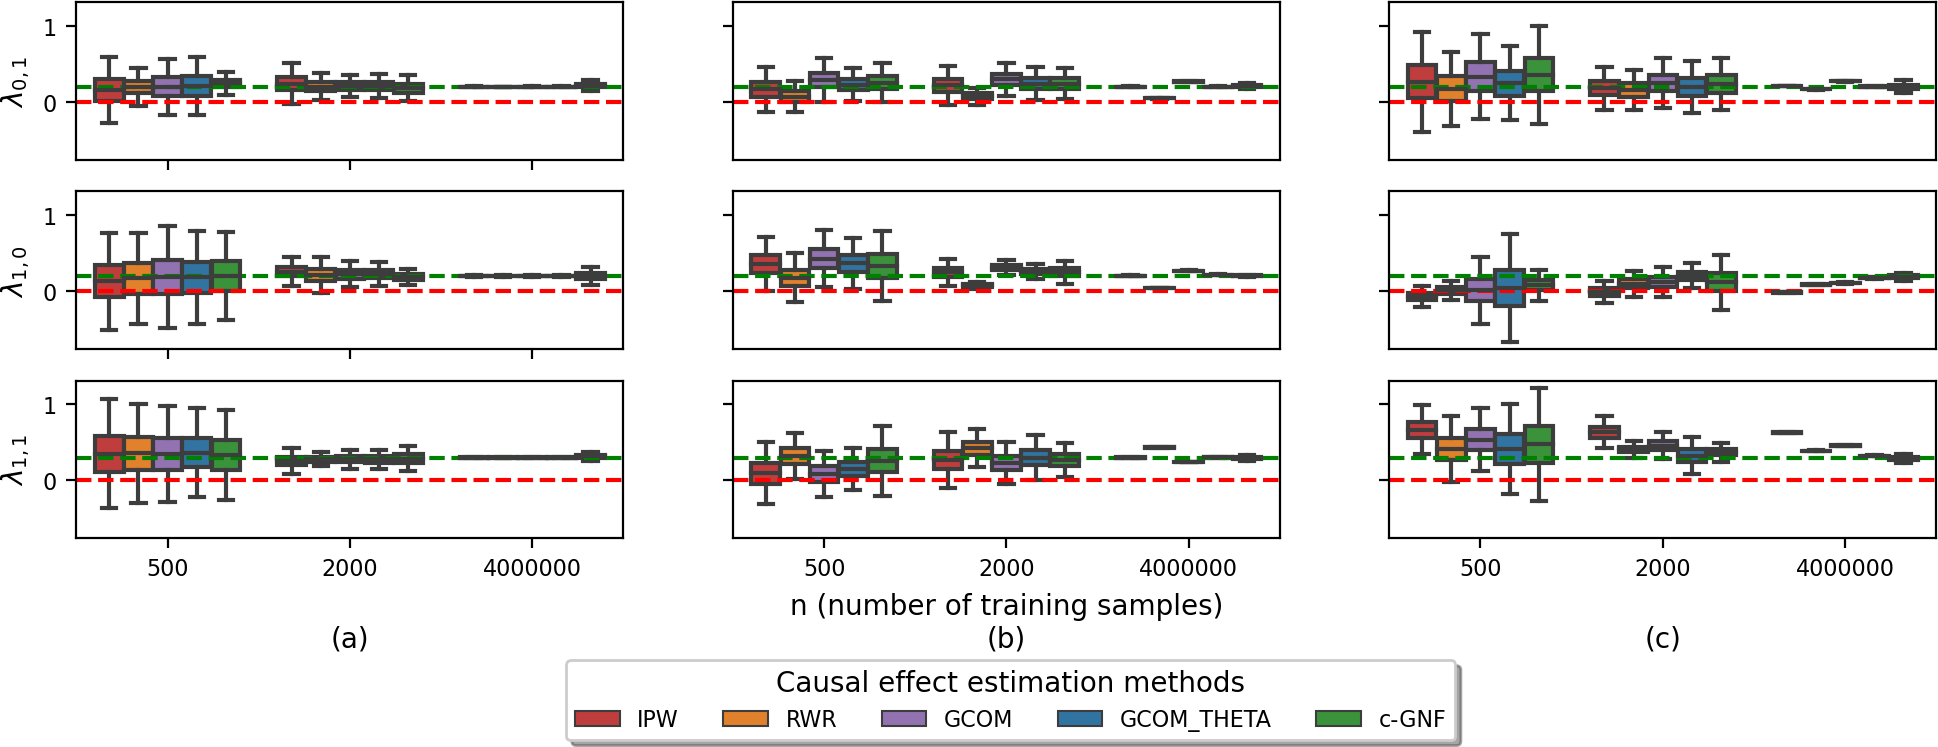
\includegraphics[width=\linewidth,keepaspectratio]{images/Tables1234_fn_theta_GNF_GCOM_IPW_RWR_200dpi.png}%_1200dpi
    \caption{
% (a) Both treatment and outcome models are correctly specified without data heterogeneity.
% (b) Only correct treatment model assumption is satisfied but the outcome model is severely misspecified with data heterogeneity.
% (c) Both outcome and treatment models are severely misspecified with data heterogeneity.
(a) $\{\theta_{11}{ = }\theta_{21}{ = }0,\gamma_{21}{ = }\gamma_{12}{ = }0\}$. (b) $\{\theta_{11}{ = }\theta_{21}{ = }0.2,\gamma_{21}{ = }0.4,\gamma_{12}{ = }0\}$. (c) $\{\theta_{11}{ = }\theta_{21}{ = }0.2,\gamma_{21}{ = }\gamma_{12}{ = }0.4\}$.
% The boxplots indicate mean, $\pm$std and $\pm$3*std of different ACE estimation methods GCOM, IPW, RWR and c-GNF for 5 random-seeded experiments across different number of training sample size. 
% In (a), all methods are on-par in terms of both asymptotic and non-asymptotic bias and variance. Especially in the case of small sample size, c-GNF outperforms other methods. In (b), as the outcome model is assumed to be incorrectly specified, GCOM and RWR result in high bias and variance estimates. Even though, IPW is unbiased, the variance is higher than c-GNF. Hence, when the correct functional forms of the outcome is unknown, IPW and c-GNF are preferred. In contrast to GCOM, assuming the correct outcome functional forms, resulting in GCOM\_THETA shows improved performance over GCOM.
% In (c), we assume both the treatment and outcome model functional forms are unknown or misspecified. As it is clearly evident, c-GNF outperforms GCOM, IPW and RWR without making any assumptions of the functional forms as the model is paramterized by a learnable deep neural network. With c-GNF we not only achieve the desirable smaller bias and variance in the ACE estimates without making any functional form assumptions, we also obtain the added advantage of utilizing c-GNF as the underlying Structural Causal Model (SCM) to perform counterfactual inference with the steps of abduction, action/intervention and deduction/prediction.
}
    \label{fig:GNF main results}
    \end{center}
% \end{sidewaysfigure}
\end{figure*}
% \begin{figure}[ht!]
% % \begin{subfigure}[b]{0.3\textwidth}
%     % \centering
%     % \begin{center}
% % \includegraphics[width=\linewidth,height=\linewidth,keepaspectratio]{images/_best_val_DAG.png}
% % \includegraphics[width=\linewidth,height=\linewidth,keepaspectratio]{images/pmf_025_075_flow_density_e20_00312.png}
% % \includegraphics[width=\linewidth,height=\linewidth,keepaspectratio]{images/pmf_050_050_flow_density_e20_00219.png}
% % \includegraphics[width=\linewidth,height=\linewidth,keepaspectratio]{images/pmf_090_010_flow_density_e20_00210.png}
% % \includegraphics[width=\linewidth,height=\linewidth,keepaspectratio]{images/Table1_GNF_GCOM_IPW_RWR.png}
% % \includegraphics[width=\linewidth,height=\linewidth,keepaspectratio]{images/Tables23_GNF_GCOM_IPW_RWR.png}
% % \includegraphics[width=\linewidth,height=\linewidth,keepaspectratio]{images/Tables23_GNF_GCOM_IPW_RWR_missing_wrong.png}
% % \includegraphics[width=\linewidth,height=\linewidth,keepaspectratio]{images/potential_outcome_map.png}
% % \includegraphics[width=\linewidth,height=\linewidth,keepaspectratio]{images/potential_outcome_maP_aio.png}
% % \includegraphics[width=\linewidth,height=\linewidth,keepaspectratio]{images/optimal_treatments.png}
% % \includegraphics[width=\linewidth,height=\linewidth,keepaspectratio]{images/optimal_treatments_1.png}
% \includegraphics[width=\linewidth,height=\linewidth,keepaspectratio]{images/optimal_treatments_2.png}
%     \caption{The frequency of the optimal treatment obtained for the 2000 data-samples from the simulated experiments. Using the potential outcome map obtained from the first law of causal inference, we can propose individual-level optimal treatments which can be viewed as personalised individual policy instead of a one-size-fits-all policy.}
%     \label{fig:personalized optimal treatment}
%     %  \end{center}
%     %  \end{subfigure}
% \end{figure}

% Earlier real-world data based work in identifying and estimating the causal effect of time-varying confounders such as \cite{wodtke2011ipw} has produced significant results in terms of analysing problem of social impact such as the effect of neighborhood on the probability of high-school graduation. However, the causal estimates in \cite{wodtke2011ipw} cannot be considered the gold standard for benchmarking causal effect estimation methods as the authenticity of the estimated causal effects cannot be verified against the true causal effect since the true causal effect is always hidden/unknown in real-world. As a result, to authenticate the estimates first task would be to know the true value that can be used as a benchmark to compare several competing causal effect estimation methods. 
% Towards this end, \cite{wodtke2020rwr} achieves the goal by experimenting on the simulated data where the true causal effect is known/calculated.
% To be consistent, we use the same simulated data generation functions to generate observational data which is used to estimate the underlying causal effect.
% We conduct all the experiments by re-implement IPW and RWR estimation code in python as the original code is based on STATA which to some extent is quite limited to the field of sociology and computational social science.
% We not only verify IPW and RWR results in python to be consistent with the results reported in~\cite{wodtke2020rwr} using STATA, but we also experiment with GCOM~\cite{kunzel2019metalearners} by modeling the outcome based on the causal identification non-parametric expression identified from $do$-calculus or $G$-computation formula. 
% Finally, we present the results from our proposed method c-GNF using deep-learning framework~\cite{paszke2017pytorch} and demonstrate the efficacy of c-GNF is not just estimating the ACEs with low bias and variance on both small and large sample size, but we also demonstrate the we can perform full counterfactual inference using the first law of causal inference~\cite{pearl2018bookofwhy} to be able to infer individual-level personalized treatments/policies.
% experiment with the neural networks based Graphical Normalizing Flows (GNFs)~\cite{wehenkel2020GNF} which can be viewed as a generalized form of Normalizing Flows that naturally presents the innate property of SEM/SCM/FCM that is used for causal inference and counterfactuals. 

For our experiments and benchmarking, we simulate a virtual social system using the $2$-wave model shown in Fig.~\ref{sfig:nh_mechanism 2-wave}. We generated continuous covariates {($C_1, C_2$)}, binary treatments {($A_1, A_2$)} and a continuous outcome  $Y$.
To provide a realistic sense to the virtual social system under our study, {($C_1, C_2$)} can denote the neighborhood contexts, e.g., the parental income of the individual in the given neighborhood, and {($A_1, A_2$)} can represents neighborhood exposures, e.g., rich/poor neighborhood, and $Y$ can represent the total score obtained in high-school graduation examination.
Our aim is to analyse the neighborhood effects on the high-school graduation.
We use the following governing equations from~\citet{wodtke2020rwr} to simulate the dataset.
\begin{IEEEeqnarray}{rCl}
C_1 & \sim & \mathcal{N}(\mu{ = }0, \sigma^2{ = }1)\enspace, \IEEEyesnumber\IEEEyessubnumber*
\label{eq:c1}\\
A_1 & \sim & {Bern}(p{ = }\Phi(0.4C_1+2\gamma_{12}C^2_1))\enspace,
\label{eq:a1gc1}\\
            % P_A1 = norm.cdf(0.4*c1.numpy()+0.6*c1.numpy()**2)
            % P_A2 = norm.cdf(0.2*a1.numpy()+0.4*c2.numpy()+0.2*a1.numpy()**2+0.4*c2.numpy()**2+0.1*a1.numpy()*c1.numpy())
C_2 & \sim & \mathcal{N}(\mu{ = }0.4C_1+0.2A_1, \sigma^2{ = }1)\enspace,
\label{eq:c2gc1a1}\\%\IEEEnonumber\\
% & & 
A_2 & \sim & {Bern}(p{ = }\Phi(0.2A_1+0.4C_2+\gamma_{12}A^2_1 \IEEEnonumber\\
& & +2\gamma_{12}C_2+\gamma_{12}C_1A_1/2))\enspace,\IEEEyessubnumber*
\label{eq:a2gc2a1}\\
Y & \sim & \mathcal{N}(\mu{ = }0.4(C_1{ - }\mu_{C_1})+A_1(0.2+\theta_{11}C_1)\IEEEnonumber*\\%\IEEEnonumber*\\
% & & 
& & +(C_2{ - }\mu_{C_2})(0.4+\gamma_{21}C_1)\IEEEnonumber*\\
& & +A_2(0.2+\theta_{21}C_1+0.1A_1),\sigma^2{ = }1)\enspace,\IEEEyessubnumber*
\label{eq:ygc1a1c2a2}% \IEEEnonumber*\\
% & & 
% & = & b_{11} \IEEEyessubnumber*\\
% & = & b_{12} \\
% & = & b_{13} \IEEEyesnumber\\
% & = & b_{14} \\
% & = & b_{15}
\end{IEEEeqnarray}
% \begin{IEEEeqnarray*}{rCl}
% C_1 & \sim & \mathcal{N}(\mu_{C_1}{ = }0, \sigma^2_{C_1}{ = }1)\enspace, \IEEEyessubnumber*
% \label{eq:c1}\\
% C_2|C_1,A_1 & \sim & \mathcal{N}(\mu_{C_2|C_1,A_1}{ = }0.4C_1+0.2A_1, \IEEEnonumber\\
% & & \sigma^2_{C_2|C_1,A_1}{ = }1)\enspace,
% \label{eq:c2gc1a1}\\
% A_1|C_1 & \sim & {Bern}(P_{A_1|C_1}{ = }\Phi(0.4C_1))\enspace,
% \label{eq:a1gc1}\\
% A_2|C_2,A_1 & \sim & {Bern}(P_{A_2|C_2,A_1}{ = }\IEEEnonumber*\\
% & & \Phi(0.2A_1+0.4C_2))\enspace,\IEEEyessubnumber*
% \label{eq:a2gc2a1}\\
% Y|C_1,A_1,C_2,A_2 & \sim & \mathcal{N}(\mu_{Y|C_1,A_1,C_2,A_2}{ = }0.4(C_1{ - }\mu_{C_1})\IEEEnonumber*\\
% & & +A_1(0.2+\theta_{11}C_1)\IEEEnonumber*\\
% & & +(C_2{ - }\mu_{C_2|C_1,A_1})(0.4+\gamma_{21}C_1)\IEEEnonumber*\\
% & & +A_2(0.2+\theta_{21}C_1+0.1A_1)), \IEEEnonumber*\\
% & & \sigma^2_{Y|C_1,A_1,C_2,A_2}{ = }1)\enspace,\IEEEyessubnumber*
% \label{eq:ygc1a1c2a2}
% % & = & b_{11} \IEEEyessubnumber*\\
% % & = & b_{12} \\
% % & = & b_{13} \IEEEyesnumber\\
% % & = & b_{14} \\
% % & = & b_{15}
% \end{IEEEeqnarray*}
where $\Phi$ is the standard normal cumulative distribution function, $\{\theta_{11},\theta_{21}\}$ are the parameters used to modify the magnitude of the causal effect modification/heterogeneity, and $\{\gamma_{12},\gamma_{21}\}$ are the parameter used to control the misspecification of the treatment and outcome models. %modify the associational effects of the confounder in different simulations. 

In the work by~\citet{wodtke2020rwr}, every experimental setting is run for 10000 randomly seeded simulations with [500, 1000, 2000] training samples (typical for social science experiments) in each simulation to report the mean ($\mu_{\lambda_{a_1,a_2}}$) and standard-deviation ($\sigma_{\lambda_{a_1,a_2}}$).
% , i.e., the ACE estimates are obtained with an effective training sample size of 2e3*1e4=2e7 analysing the asymptotic bias and variance of the ACE estimates. 
% However, in most practical cases typical to social sciences, the effective training sample size ranges only from few hundreds to thousands and, thus, we need to evaluate not just asymptotic means and variances but also non-asymptotic ones. 
However, in most practical cases, it is atypical to run deep neural networks for 10000 simulations and is limited between one to 10 in most practical deep learning applications. 
Hence, we run our experiments with different samples sizes for five randomly seeded simulations,
%, i.e., effective sample size in range 25e2-2e7 
using all the methods (IPW, RWR, GCOM and c-GNF) and report the results pictorially in Fig.~\ref{fig:GNF main results}.
% We repeat every experiment with 5 random seeds in order to observe and report the bias and variance of the causal effect estimates across IPW, RWR, GCOM and c-GNF. 
Since we run multiple simulations with multiple setting with c-GNFs, we do not concentrate on hyperparameter selection that is best for each simulation and simply use three fully-connected layers with [20, 15, 10] hidden units for the graphical conditioner and three fully-connected layers with [15, 10, 5] hidden units for the monotonic UMNN transformer.
We implement c-GNFs in Pytorch~\cite{paszke2017pytorch} using GNF baseline code\footnote{\url{https://github.com/AWehenkel/Graphical-Normalizing-Flows}} and AdamW~\cite{LoshchilovH2019adamw} optimizer with learning-rate=$1e{-3}$ and a batch-size of 128 (2GB of GPU memory) for all our experiments.
It is also our aim to evaluate the robustness of c-GNFs in estimating the ACEs without any fine hyperparameters selection using only the most basic/default settings.
Since, deep neural networks are prone to overfit, we split our data into three train, validation and test sets in ratio 8:1:1. We strictly use only the training set with [500, 2000, 4000000] samples for training and use the held-out validation set for early stopping to get the model with best validation loss. 
We further validate the generalization of the best validation loss model on the held-out test set.
We simulate 2000 samples from every interventional distributions using c-GNFs to evaluate $\mathbf{E}[Y_{a_1,a_2}]$ to obtain Monte-Carlo estimates of ACEs using Eqs.~\eqref{eq:lambda10}-\eqref{eq:lambda11}. Theoretically, a higher number of samples from the interventional distributions would provide better Monte-Carlo estimates at an added computational cost.
% experiment with the neural networks based Graphical Normalizing Flows (GNFs)~\cite{wehenkel2020GNF} which can be viewed as a generalized form of Normalizing Flows that naturally presents the innate property of SEM/SCM/FCM that is used for causal inference and counterfactuals. 
% In the description of the experiments, I don't get what you mean by effective training sample and why this is important. I also find confussing that you start saying that you simulate 2000 samples but then run experiments with 500-2000 samples (I get that you simulate 2000 and then selects subsets of different sizes out of these 2000, but I think it is common to say that produce samples of sizes 500,.., 2000). Then, you also have to mention that 0, 0.2 and 0.5 are the true causal effects for the model simulated and, thus, you compute the true lambdas as you mention.

Fig.~\ref{fig:GNF main results} indicates the results for the following three experimental settings: 
\begin{inparaenum}[(i)]
\item Fig.~\ref{fig:GNF main results}a shows the results with both the treatment and outcome models correctly specified without heterogeneity in data.
\item Fig.~\ref{fig:GNF main results}b shows the results with only the treatment model correctly specified with heterogeneity in data.
\item Fig.~\ref{fig:GNF main results}c shows the results with both treatment and outcome models misspecified with heterogeneity in data.
\end{inparaenum}
Under all three experimental settings, the true ACEs of interest for the above $2$-wave time-varying model $\lambda_{a_1,a_2}$ for the binary treatments $\{{A_1}{ := }a_1, {A_2}{ := }a_2\}$ are calculated from Eqs.~\eqref{eq:lambda01}-\eqref{eq:lambda11} as $\lambda_{1,0}{ = }{0.2{ - }0}{ = }0.2, \lambda_{0,1}{ = }{0.2{ - }0}{ = }0.2$, and $\lambda_{1,1}{ = }{0.5{ - }0.2}{ = }0.3$ and denoted by green horizontal dotted lines in Fig.~\ref{fig:GNF main results}.
The red horizontal dotted line in Fig.~\ref{fig:GNF main results} represents \emph{zero}-ACE which can be considered as the critical point due to the fact that \emph{zero}-ACE indicates both the treatments to have the same causal effect/outcome. Sometimes, it is more important to accurately identify the sign of the ACE with some acceptable tolerance in the magnitude of the ACE estimate as the sign is what determines the effectiveness of the treatment, e.g., $\lambda_{1,0}{ > }0$ in Eq.~\eqref{eq:lambda10} indicates treatment $\{{A_1}{ := }1, {A_2}{ := }0\}$ is better than treatment $\{{A_1}{ := }0, {A_2}{ := }0\}$ in expectation, and vice-versa if $\lambda_{1,0}{ < }0$. It is of primary importance to identify which treatment is better and of secondary importance to identify by what amount the treatment is better, in expectation.
In Fig.~\ref{fig:GNF main results}, the box-plots indicate {$\mu, \mu{ \pm }\sigma,\mu{ \pm }3\sigma$} values for all $\lambda_{a_1,a_2}$ to provide an idea of the variance of the estimates.
Observe that in all the plots, c-GNF does not include the \emph{zero}-ACE in $\mu{ \pm }\sigma$ range indicating that c-GNF does not introduce ambiguity in the selection of best treatment, in expectation, unlike IPW, RWR and GCOM. This non-ambiguity is a desired quality from any causal effect estimation methods used in decision-making.

In Fig.~\ref{fig:GNF main results}a, we see that all the models perform equally well under no model misspecification and effect modification/heterogeneity in data.
However increasing the complexity by adding outcome model misspecification and data heterogeneity in Fig.~\ref{fig:GNF main results}b, we see that the regression based outcome methods not assuming the right functional forms, i.e., GCOM and RWR, result in biased estimates in both small and large samples. 
% The bias in GCOM due to outcome model misspecification can be corrected by assuming the right function forms of the outcome model in GCOM by including the terms corresponding to $\{\theta_{12},\theta_{21}\}$ to obtain the unbiased ACE estimate denoted as {GCOM\_THETA} in Fig.~\ref{fig:GNF main results}. 
{GCOM\_THETA} in Fig.~\ref{fig:GNF main results} refers correcting GCOM by specifying the true functional form manually or parameterizing the model by a deep neural network as in the case of meta-learners to result in unbiased estimates.
Hence, we see that {GCOM\_THETA} performs better than {GCOM} due to the correction.
Similarly, since the treatment model is rightly specified, IPW estimates are unbiased. 
% However, c-GNF also provides unbiased estimates with lesser variance compared to IPW.
In contrast to Figs.~\ref{fig:GNF main results}a and \ref{fig:GNF main results}b, Fig.~\ref{fig:GNF main results}c indicates the treatment model is misspecified as well. With the treatment model misspecified, IPW no longer results in unbiased estimates.
From Fig.~\ref{fig:GNF main results}, we show that in small-sample size regime, c-GNF results in unbiased estimates with comparable variance.
We can still do better in terms of variance by appropriate selection of the deep neural networks as a part of the hyperparameter tuning, which is not our aim.
% We also show the estimates are unbiased with small variance in large-sample size due to the underfitting which can be fixed by appropriate selecting the size of the deep neural networks as a part of the hyperparameter tuning.
% The technical appendix also reports experiments with sample sizes [1000, 4000, 40000, 400000].
% Additional experiments with sample sizes [1000, 4000, 40000, 400000] are reported in the technical appendix.
A real-world application of c-GNF on a large-scale non-randomized observational study to analyse the impact of IMF (International Monetary Fund) program on the child poverty is conducted in~\citet{balgi2022counterfactual} that observes an effective reduction of child poverty by $1.2{\pm}0.24$ degrees in the Global-South, thus indicating the beneficial nature of IMF program on child poverty reduction.


% \begin{inparaenum}

% \item \textbf{$\{\theta_{11}{ = }\theta_{21}{ = }0,\gamma_{21}{ = }\gamma_{12}{ = }0\}$}: Fig.~\ref{fig:GNF main results}a shows the results with both the treatment and outcome models correctly specified without heterogeneity in data. %, i.e., $\{\theta_{11}{ = }\theta_{21}{ = }0,\gamma_{12}{ = }\gamma_{21}{ = }0\}$,
% In Fig.~\ref{fig:GNF main results}a, we observe that for all the methods the asymptotic mean and variance are similar when there is no heterogeneity in data. However as previously mentioned, asymptotic behavior can be considered theoretical and usually not achievable in practical scenarios where the sample size is limited to typically few thousands. So, under small sample size of 500-1000, c-GNF is better as all other methods encapsulate zero-ACE in range of $\mu_{\lambda_{a_1,a_2}}\pm\sigma_{\lambda_{a_1,a_2}}$. The small bias in c-GNF relative to other methods at low samples can be attributed to small overfitting of the neural-network for small sample size, which can be addressed with additional fine tuning of the hyperparameters. 
% % In addition to exploring the effect of sample size on the ACE estimates, we also analyse the robustness to handle effect modification/heterogeneity~\cite{vanderweele2009effectmodification_interaction} in the training data and also the outcome and/or treatment model misspecifications.
% Under all three experimental settings, the true ACEs of interest for the above $2$-wave time-varying model $\lambda_{a_1,a_2}$ for the binary treatments $\{{A_1}{ := }a_1, {A_2}{ := }a_2\}$ are calculated as $\lambda_{1,0}{ = }{0.2{ - }0}{ = }0.2, \lambda_{0,1}{ = }{0.2{ - }0}{ = }0.2$, and $\lambda_{1,1}{ = }{0.5{ - }0.2}{ = }0.3$ and denoted by green horizontal dotted lines in Fig.~\ref{fig:GNF main results}.
% In Fig.~\ref{fig:GNF main results}, the red horizontal dotted line represents zero-ACE which can be considered as the critical point due to the fact that zero-ACE indicates both the treatments to have the same causal effect/outcome. Sometimes, it is more important to accurately identify the sign of the ACE with some acceptable tolerance in the magnitude of the ACE estimate as the sign is what determines the effectiveness of the treatment, e.g., $\lambda_{1,0}{ > }0$ in~\eqref{eq:lambda10} indicates treatment $A_1{ = }1,A_2{ = }0$ is better than treatment $A_1{ = }0,A_2{ = }0$ in expectation, and vice-versa if $\lambda_{1,0}{ < }0$. It is of primary importance to identify which treatment is better and secondary importance to identify by what amount the treatment is better, in expectation.

% % Jose: I am afraid that I don't see that c-GNF is better for small sample sizes. I wouldn't use the word "encapsulate" in this context, e.g. replace with "include".

% \item \textbf{$\{\theta_{11}{ = }\theta_{21}{ = }0.2,\gamma_{21}{ = }0.4,\gamma_{12}{ = }0\}$}: Fig.~\ref{fig:GNF main results}b shows the results with only the treatment model correctly specified with heterogeneity in data. %, i.e., $\{\theta_{11}{ = }\theta_{21}{ = }0.2,\gamma_{12}{ = }0,\gamma_{21}{ = }0.4\}$, and
% In Fig.~\ref{fig:GNF main results}b, under effect modification/heterogeneity in data and outcome model misspecification, we observe that the outcome modeling methods RWR and GCOM result in biased estimates both in small and large sample sizes. The bias in GCOM due to outcome model misspecification can be corrected by assuming the right function forms of the outcome model in GCOM by including the terms corresponding to $\{\theta_{12},\theta_{21}\}$ to obtain the unbiased ACE estimate denoted as {GCOM\_THETA} in Fig.~\ref{fig:GNF main results}. 
% The {GCOM\_THETA} refers to enhancing GCOM by specifying the true function form manually or parameterizing the model by a deep neural network as in the case of meta-learners~\cite{kunzel2019metalearners}.
% Hence, we see that {GCOM\_THETA} performs better than {GCOM} due to the enhancement.
% Since the treatment model is rightly specified, IPW estimates are unbiased. However, c-GNF also provides unbiased estimates with lesser variance compared to IPW.


% \item \textbf{$\{\theta_{11}{ = }\theta_{21}{ = }0.2,\gamma_{21}{ = }\gamma_{12}{ = }0.4\}$}: Fig.~\ref{fig:GNF main results}c shows the results with both treatment and outcome models misspecified with heterogeneity in data. %, i.e., $\{\theta_{11}{ = }\theta_{21}{ = }0.2,\gamma_{12}{ = }\gamma_{21}{ = }0.4\}$. In Fig.~\ref{fig:GNF main results}c, we present the experiments with both treatment and outcome models are misspecified and the data also exhibits heterogeneity.
% Unsurprisingly under the outcome and treatment model misspecification, we find that IPW, GCOM and RWR all result in biased estimates. However, as c-GNF does not require any functional form assumptions, it is able to model the data distribution and its underlying SCM resulting in unbiased estimates or least biased estimates. We can also observe that with larger effective sample size and a bigger neural-network, c-GNF highlights another benefit compared to the other methods. Note that even though GCOM\_THETA is observed to result in unbiased estimates, this is because the right parameteric functional forms are assumed. However, in most practical applications, particularly in the social sciences, the right functional forms are almost always unknown. Hence in applied social-science research, c-GNF should outperform standard statistical techniques such as IPW, RWR, and GCOM. The relevance of c-GNF increases as the size of social science data is inflating and as the availability of computational resources is becoming cheaper.

% % Jose: Honestly, I don't see that c-GNF outperforms the other methods. I would say that it is on par. The main (huge) advantage is that c-GNF does it without having to specify the functional form.
% \end{inparaenum}

% \section{Results and Discussion}\label{sec:results}

\subsection{Counterfactual Inference}
\begin{figure}[ht!]
    % \centering
    %  \begin{subfigure}[b]{0.6\textwidth}
    %  \begin{center}
% \includegraphics[width=\linewidth,height=\linewidth,keepaspectratio]{images/_best_val_DAG.png}
% \includegraphics[width=\linewidth,height=\linewidth,keepaspectratio]{images/pmf_025_075_flow_density_e20_00312.png}
% \includegraphics[width=\linewidth,height=\linewidth,keepaspectratio]{images/pmf_050_050_flow_density_e20_00219.png}
% \includegraphics[width=\linewidth,height=\linewidth,keepaspectratio]{images/pmf_090_010_flow_density_e20_00210.png}
% \includegraphics[width=\linewidth,height=\linewidth,keepaspectratio]{images/Table1_GNF_GCOM_IPW_RWR.png}
% \includegraphics[width=\linewidth,height=\linewidth,keepaspectratio]{images/Tables23_GNF_GCOM_IPW_RWR.png}
% \includegraphics[width=\linewidth,height=\linewidth,keepaspectratio]{images/Tables23_GNF_GCOM_IPW_RWR_missing_wrong.png}
% \includegraphics[width=\linewidth,height=\linewidth,keepaspectratio]{images/potential_outcomes_map.png}
\centering
\begin{subfigure}[t]{0.45\textwidth}
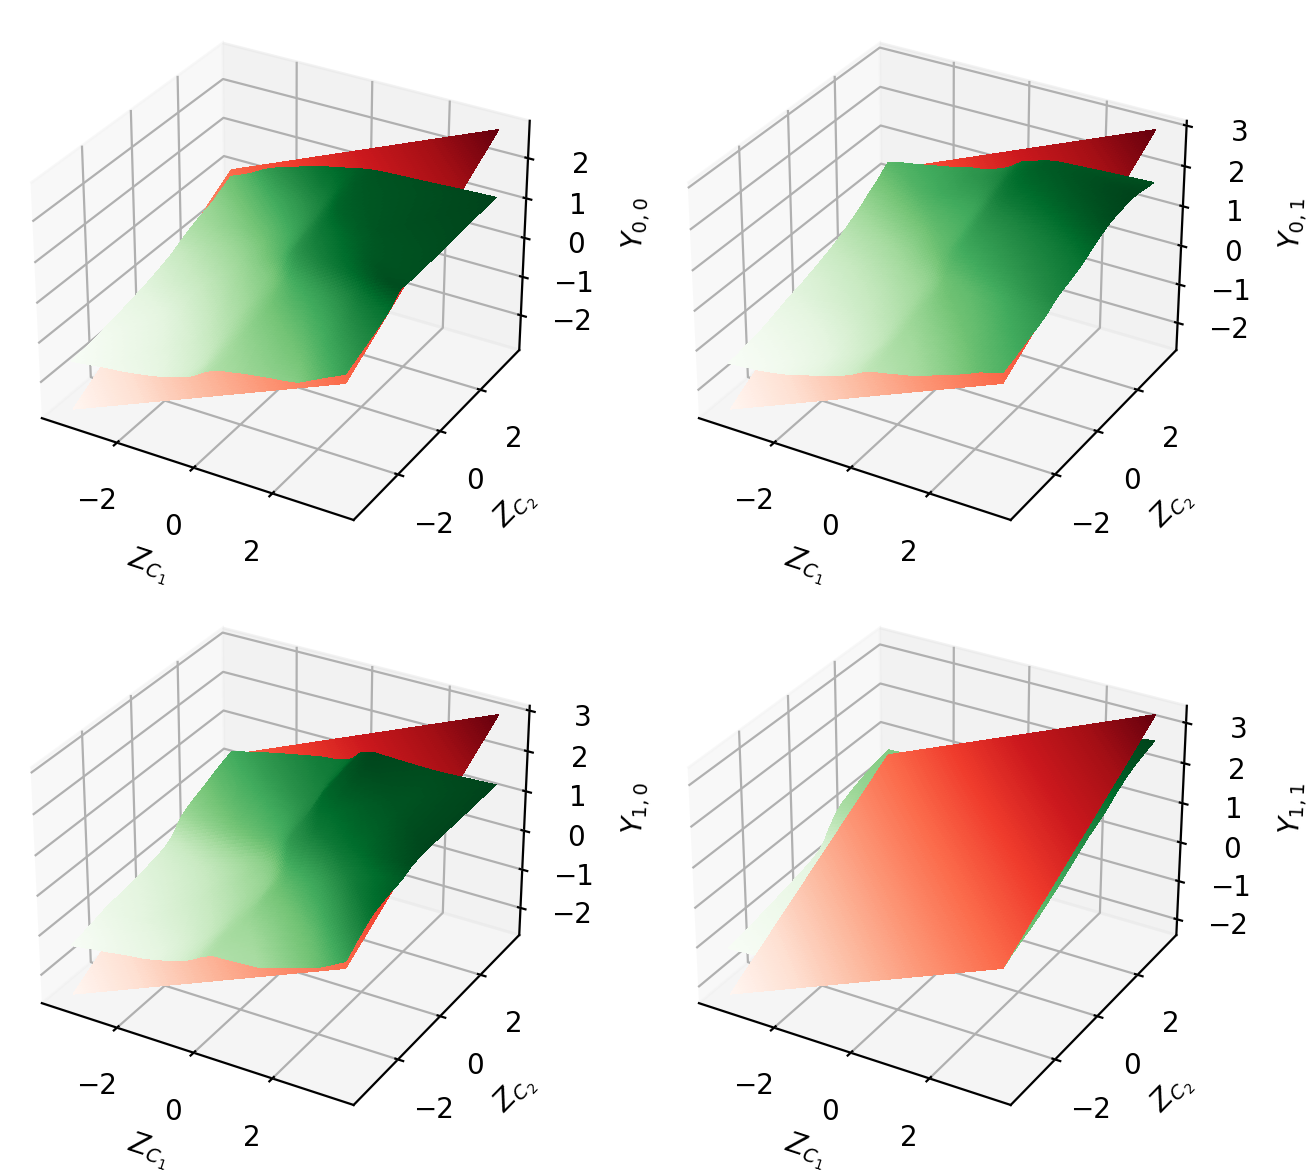
\includegraphics[width=\linewidth,height=\linewidth,keepaspectratio]{images/potential_outcomes_map_s1_new.png}
\caption{}
    \label{sfig:potential outcomes map}
\end{subfigure}
% \begin{subfigure}[t]{0.45\textwidth}
% \includegraphics[width=\linewidth,height=\linewidth,keepaspectratio]{images/optimal_treatments_2_dpi300.png}
%     \caption{Armed with the potential outcomes map, we can deduce optimal individual-level personalized treatment/policy $\bar{a}_1\bar{a}_2{ = }\argmax_{a_1a_2} Y_{a_1,a_2}$. The frequency of the optimal treatments obtained for the 2000 data-samples from the simulated experiments. 
%     }
%     \label{sfig:personalized optimal treatment}
% \end{subfigure}
\hfill
\centering
\begin{subfigure}[t]{0.23\textwidth}

\includegraphics[width=\linewidth,height=\linewidth,keepaspectratio]{images/confmat_val_s1_new.png}
    \caption{}
    \label{sfig:personalized optimal treatment val}
\end{subfigure}
\hfill
\centering
\begin{subfigure}[t]{0.23\textwidth}

\includegraphics[width=\linewidth,height=\linewidth,keepaspectratio]{images/confmat_tst_s1_new.png}
    \caption{}
    \label{sfig:personalized optimal treatment tst}
\end{subfigure}
\hfill
% \includegraphics[width=\linewidth,height=\linewidth,keepaspectratio]{images/potential_outcome_maP_aio.png}
% \includegraphics[width=\linewidth,height=\linewidth,keepaspectratio]{images/optimal_treatments.png}
% \includegraphics[width=\linewidth,height=\linewidth,keepaspectratio]{images/optimal_treatments_1.png}
% \includegraphics[width=\linewidth,height=\linewidth,keepaspectratio]{images/optimal_treatments_2.png}
    % \caption{The complete map of all 4 potential outcomes $Y_{a_1,a_2}{ = }\{Y_{0,0},Y_{0,1},Y_{1,0},Y_{1,1}\}$ obtained from the first law of causal inference~\cite{pearl2018bookofwhy}, i.e., (i) abduction, (ii) action, and (iii) prediction.
    % Armed with the potential outcomes map, we can deduce optimal individual/personalized treatments $a_1a_2=\argmax_{a_1a_2} Y_{a_1,a_2}$ .
    % % Since c-GNF offers both density/likelihood estimation and data sampling, we can estimate likelihood of a given data-sample and even sample new data from observational or any possible interventional distribution.
    % }
    %  \end{center}
    %  \end{subfigure}
%      \hfill
%      \begin{subfigure}[b]{0.45\textwidth}
%     \centering
% % \includegraphics[width=\linewidth,height=\linewidth,keepaspectratio]{images/_best_val_DAG.png}
% % \includegraphics[width=\linewidth,height=\linewidth,keepaspectratio]{images/pmf_025_075_flow_density_e20_00312.png}
% % \includegraphics[width=\linewidth,height=\linewidth,keepaspectratio]{images/pmf_050_050_flow_density_e20_00219.png}
% % \includegraphics[width=\linewidth,height=\linewidth,keepaspectratio]{images/pmf_090_010_flow_density_e20_00210.png}
% % \includegraphics[width=\linewidth,height=\linewidth,keepaspectratio]{images/Table1_GNF_GCOM_IPW_RWR.png}
% % \includegraphics[width=\linewidth,height=\linewidth,keepaspectratio]{images/Tables23_GNF_GCOM_IPW_RWR.png}
% % \includegraphics[width=\linewidth,height=\linewidth,keepaspectratio]{images/Tables23_GNF_GCOM_IPW_RWR_missing_wrong.png}
% % \includegraphics[width=\linewidth,height=\linewidth,keepaspectratio]{images/potential_outcome_map.png}
% \includegraphics[width=\linewidth,height=\linewidth,keepaspectratio]{images/potential_outcomes_maP_aio.png}
% % \includegraphics[width=\linewidth,height=\linewidth,keepaspectratio]{images/optimal_treatments.png}
% % \includegraphics[width=\linewidth,height=\linewidth,keepaspectratio]{images/optimal_treatments_1.png}
% % \includegraphics[width=\linewidth,height=\linewidth,keepaspectratio]{images/optimal_treatments_2.png}
%     \caption{Caption}
%     \label{fig:my_label}
%      \end{subfigure}
% \end{figure*}
% \begin{figure*}
%     \centering
%      \begin{subfigure}[b]{0.3\textwidth}
% % \includegraphics[width=\linewidth,height=\linewidth,keepaspectratio]{images/_best_val_DAG.png}
% % \includegraphics[width=\linewidth,height=\linewidth,keepaspectratio]{images/pmf_025_075_flow_density_e20_00312.png}
% % \includegraphics[width=\linewidth,height=\linewidth,keepaspectratio]{images/pmf_050_050_flow_density_e20_00219.png}
% % \includegraphics[width=\linewidth,height=\linewidth,keepaspectratio]{images/pmf_090_010_flow_density_e20_00210.png}
% % \includegraphics[width=\linewidth,height=\linewidth,keepaspectratio]{images/Table1_GNF_GCOM_IPW_RWR.png}
% % \includegraphics[width=\linewidth,height=\linewidth,keepaspectratio]{images/Tables23_GNF_GCOM_IPW_RWR.png}
% % \includegraphics[width=\linewidth,height=\linewidth,keepaspectratio]{images/Tables23_GNF_GCOM_IPW_RWR_missing_wrong.png}
% % \includegraphics[width=\linewidth,height=\linewidth,keepaspectratio]{images/potential_outcome_map.png}
% % \includegraphics[width=\linewidth,height=\linewidth,keepaspectratio]{images/potential_outcome_maP_aio.png}
% \includegraphics[width=\linewidth,height=\linewidth,keepaspectratio]{images/optimal_treatments.png}
% % \includegraphics[width=\linewidth,height=\linewidth,keepaspectratio]{images/optimal_treatments_1.png}
% % \includegraphics[width=\linewidth,height=\linewidth,keepaspectratio]{images/optimal_treatments_2.png}
%     \caption{Caption}
%     \label{fig:my_label}
%      \end{subfigure}
%      \hfill
%      \begin{subfigure}[b]{0.3\textwidth}
%     \centering
% % \includegraphics[width=\linewidth,height=\linewidth,keepaspectratio]{images/_best_val_DAG.png}
% % \includegraphics[width=\linewidth,height=\linewidth,keepaspectratio]{images/pmf_025_075_flow_density_e20_00312.png}
% % \includegraphics[width=\linewidth,height=\linewidth,keepaspectratio]{images/pmf_050_050_flow_density_e20_00219.png}
% % \includegraphics[width=\linewidth,height=\linewidth,keepaspectratio]{images/pmf_090_010_flow_density_e20_00210.png}
% % \includegraphics[width=\linewidth,height=\linewidth,keepaspectratio]{images/Table1_GNF_GCOM_IPW_RWR.png}
% % \includegraphics[width=\linewidth,height=\linewidth,keepaspectratio]{images/Tables23_GNF_GCOM_IPW_RWR.png}
% % \includegraphics[width=\linewidth,height=\linewidth,keepaspectratio]{images/Tables23_GNF_GCOM_IPW_RWR_missing_wrong.png}
% % \includegraphics[width=\linewidth,height=\linewidth,keepaspectratio]{images/potential_outcome_map.png}
% % \includegraphics[width=\linewidth,height=\linewidth,keepaspectratio]{images/potential_outcome_maP_aio.png}
% % \includegraphics[width=\linewidth,height=\linewidth,keepaspectratio]{images/optimal_treatments.png}
% \includegraphics[width=\linewidth,height=\linewidth,keepaspectratio]{images/optimal_treatments_1.png}
% % \includegraphics[width=\linewidth,height=\linewidth,keepaspectratio]{images/optimal_treatments_2.png}
    \caption{
    (a) The red and green surface-plots respectively represent the potential outcome maps of true SCM $F$ and our \emph{encapsulated-SCM} $\tilde{F}$ generated from the SCM noise ranges $Z_{C_1}{ \in }[-3,3], Z_{C_2}{ \in }[-3,3], Z_Y{ = }0$.% in Eq.~\eqref{eq:ygc1a1c2a2},  in Eq.~\eqref{eq:first law of causal inference} 
    % (a) All four potential outcomes $Y_{a_1,a_2}$ map predicted from~\eqref{eq:first law of causal inference} using encapsulated-SCM (c-GNF) $\tilde{F}$ (green) against the true SCM $F$~\eqref{eq:ygc1a1c2a2} (red). %{ = }\{Y_{0,0},Y_{0,1},Y_{1,0},Y_{1,1}\}
    % Since c-GNF offers both density/likelihood estimation and data sampling, we can estimate likelihood of a given data-sample and even sample new data from observational or any possible interventional distribution.
    ~(b, c) Confusion matrices between the true and predicted optimal personalised policy on unseen validation and test sets respectively (with model under no misspecification setting from Fig.~\ref{fig:GNF main results}a).
    }
    \label{fig:first law of causal inference}
%      \end{subfigure}
    %  \hfill
\end{figure}
Apart from the benefits of ACE estimates with small bias and variance compared to standard statistical methods, c-GNF provides the unique benefit of counterfactual inference using \emph{`The First Law of Causal Inference'}~\cite{pearl2009abductionactionprediction, pearl2009causality, pearl2018bookofwhy}, which is virtually non-existent in IPW/RWR/GCOM. `The First Law of Causal Inference' essentially provides a framework to identify the unit level potential outcomes using SCM, thereby addressing the fundamental missing value problem of counterfactual inference. This law to identify the missing/unseen potential outcome $Y_{a_1,a_2}$ for a unit $\mathbf{Z^\ell}$ is represented mathematically as
\begin{IEEEeqnarray}{rll}
Y_{a_1,a_2}(\mathbf{Z}^\ell){ = }Y_{\tilde{F}_{a_1,a_2}}(\mathbf{Z}^\ell)\enspace,\IEEEyesnumber\label{eq:first law of causal inference}%\\
% P_\mathbf{X}(\mathbf{X}) = P_\mathbf{Z}(\mathbf{Z}) |\mathrm{det} J_{T}(\mathbf{Z})|^{-1}\enspace, \mathrm{where} \enspace \mathbf{Z}{ = }T^{-1}(\mathbf{X}).\IEEEyesnumber%\\%S_j:
% &&+a + b\\
% &&+{}a + b\\
% &&{}+a + b\\
% U_i{ \indep }U_j, \enspace i \neq j,\enspace (i,j{=}1,\ldots, d)\enspace,\label{seq:scm noise}
%  \int_{-\infty}^{\infty}\delta(x=a) = 1\label{eq:diracdeltaunitarea}\enspace,\\
\end{IEEEeqnarray}
% \begin{IEEEeqnarray}{rll}
% Y_{a_1,a_2}(\mathbf{Z}^i){ = }Y_{\tilde{F}_{a_1,a_2}}(\mathbf{Z}^i)\enspace,\IEEEyesnumber\label{eq:first law of causal inference}%\\
% % P_\mathbf{X}(\mathbf{X}) = P_\mathbf{Z}(\mathbf{Z}) |\mathrm{det} J_{T}(\mathbf{Z})|^{-1}\enspace, \mathrm{where} \enspace \mathbf{Z}{ = }T^{-1}(\mathbf{X}).\IEEEyesnumber%\\%S_j:
% % &&+a + b\\
% % &&+{}a + b\\
% % &&{}+a + b\\
% % U_i{ \indep }U_j, \enspace i \neq j,\enspace (i,j{=}1,\ldots, d)\enspace,\label{seq:scm noise}
% %  \int_{-\infty}^{\infty}\delta(x=a) = 1\label{eq:diracdeltaunitarea}\enspace,\\
% \end{IEEEeqnarray}
where $Y_{a_1,a_2}(\mathbf{Z}^\ell)$ denotes the potential outcome $Y$ under the treatments $\{{A_j}{ := }a_j\}^2_{j{ = }1}$ for a given unit individual $\mathbf{Z}^\ell$ that is fundamentally missing and is of interest for counterfactual inference, and $Y_{\tilde{F}_{a_1,a_2}}(\mathbf{Z}^\ell)$ represents the actual outcome $Y$ observed from the mutilated-SCM $\tilde{F}_{a_1,a_2}$ that is obtained by the mutilation $\{{A_j}{ := }a_j\}^2_{j{ = }1}$ on the \emph{encapsulated-SCM} $\tilde{F}$. Essentially, this law involves three steps that help identify the missing potential outcomes, thereby addressing the fundamental missing value problem of causal inference.
% \begin{enumerate}
\begin{inparaenum}

    \item \textbf{Abduction}: For a given observed unit-individual evidence $\mathbf{X}^\ell$, the respective exogenous SCM noise $\mathbf{Z}^\ell$ corresponding to $\mathbf{X}^\ell$ is recovered from the encapsulated-SCM $\tilde{F}$. In case of c-GNF, we have $\mathbf{Z}^\ell{ = }T\mathbf{X}^\ell{ = }\tilde{F}^{-1}\mathbf{X}^\ell$ where the \emph{encapsulated-SCM} noise $\mathbf{Z}^\ell$ 
   indicates the unique hidden essence/identifier/DNA
    of the $\ell^{th}$ unit-individual with observed evidence $\mathbf{X}^\ell$.
    %with a unique $\mathbf{Z}$ for every unique $\mathbf{X}$ as $T$ 
%   is bijective, i.e., $\mathbf{Z}^i{ = }\mathbf{Z}^j{ \Leftrightarrow }\mathbf{X}^i{ = }\mathbf{X}^j$, i.e., $\mathbf{Z}^\ell$ acts as a unique signature of $\mathbf{X}^\ell$.
    
    \item \textbf{Action}: The action or intervention (in our case a public policy) corresponding to the desired treatment is conducted in the form of mutilating the corresponding structural equation of the treatment $\{{A_j}{ := }a_j\}^2_{j{ = }1}$ in $\tilde{F}$ (modularity assumption) resulting in the mutilated-SCM $\tilde{F}_{a_1,a_2}$. 
    
    \item \textbf{Prediction}: The recovered noises $\mathbf{Z}^\ell$ from abduction are re-propagated through $\tilde{F}_{a_1,a_2}$ and the outcomes $Y_{\tilde{F}_{a_1,a_2}}(\mathbf{Z}^\ell)$ observed are nothing but the potential outcomes $Y_{a_1,a_2}(\mathbf{Z}^\ell)$ we were interested to begin with.% under the treatments $\{{A_j}{ := }a_j\}^2_{j{ = }1}$ for a given unit individual $\mathbf{Z}^\ell$.% from~\eqref{eq:first law of causal inference}.%outcome $Y$ observed is the potential outcome under the . 
    % Mathematically, $\mathbf{X}^i_a{ = }\tilde{F}_a\mathbf{Z}^i$ and $Y_{\tilde{F}_a}(\mathbf{Z}^i){ \in }\mathbf{X}_a^i$.
\end{inparaenum}    
% \end{enumerate}

% Jose: I find the notation above a bit cumbersome. It is not enough to use Y_a(x^i) in equation 22. Why do you have to add T_a in that equation. You sill explain this in step 2 of counterfactual inference. I don't get either why you need to introduce x^i_a in step 3, since this is essentially Y_a(x^i). You cite the book of why quite often. I consider this a popular science book. I would prefer to cite Pear's Causality book from 2009. I have send you a pdf copy.

% Fig.~\ref{sfig:potential outcomes map} represents all the four potential outcome map obtained using the three steps of counterfactual inference with our proposed method c-GNF.
The potential outcome maps in Fig.~\ref{sfig:potential  outcomes map} are generated using the three steps of counterfactual inference with c-GNF, i.e., \emph{encapsulated-SCM} and the noises $Z_{C_1}{ \in }[-3,3], Z_{C_2}{ \in }[-3,3], Z_Y{ = }0$ to observe the effect of $C_1$ and $C_2$ on $Y$.
Due to the linear nature of the structural equation in Eq.~\eqref{eq:ygc1a1c2a2} under no model misspecification setting, the true potential outcome maps are represented by the flat hyperplanes in Fig.~\ref{sfig:potential outcomes map} (red).
% ($Z$s are assumed to be standard normal noise) to observe the effect of $C_1$ and $C_2$ on $Y$, i.e., $Z_Y{ = }0$ because of limitation of 4D plot visualization and our primary interest to observe the effects of $C_1, C_2$ on $Y$.
% Also since $Y$ is a strictly monotonic function of $Z_Y$ because of UMNN transformer, the as $Z_X$ is assumed to be standard normal noise.
Observe that around the corners of the green 3D surface-plots which represents the low likelihood region of observing samples, the extrapolation assumption is slightly violated as the observational data corresponding to these regions are likely missing in the training set due to low likelihood. 
Extrapolation is an inevitable assumption made in almost all statistical models which is almost always violated under practical finite data setting.
True extrapolation can be attained only with infinite data, which is impractical and unrealistic.%practically
% However, the 
~In the technical appendix, we further present the same set of plots as in Fig.~\ref{fig:first law of causal inference} under the complex experimental setting when both the models are misspecified and also the data exhibits effect modification/heterogeneity.

The confusion matrices from unseen validation and test sets in Figs.~\ref{sfig:personalized optimal treatment val} and~\ref{sfig:personalized optimal treatment tst} indicate the true and predicted optimal individual-level treatment/policy $\bar{a}^\ell_1,\bar{a}^\ell_2$ for the $\ell^{th}$ individual $\mathbf{X}^\ell$, which is predicted as below from Eq.~\eqref{eq:first law of causal inference}
% by comparing the points on potential outcomes map corresponding to every individual, i.e., the optimal treatment $\bar{a}_1\bar{a}_2$ can be defined as
\begin{IEEEeqnarray}{rll}
\bar{a}^\ell_1,\bar{a}^\ell_2{ = }\argmax_{a_1,a_2} Y_{a_1,a_2}(T\mathbf{X}^\ell)\enspace.\IEEEyesnumber\label{eq:optimal personalized treatment}
% Jose: Figure 4 needs further explanation. Do you mean that you do counterfactual inference for each of the 2000 samples where there the prediction is for actions 00, 01, 10 and 11 ? Then, I don't get why the maps is 2-D.
\end{IEEEeqnarray}
Using c-GNF, we observe that the optimal treatments are indeed predicted with a very high accuracy of 99.6\% on unseen validation and test sets under no-misspecification and no effect modification/heterogeneity in data. 
Similarly, under both model misspecifications we obtain 91\% accuracy even with our sub-optimal hyperparameters.
Thus, c-GNF enables precise P$^3$A targeting and articulation of the tailored treatments/policies in the social sciences, instead of relying on `one-size-fits-all' sub-optimal treatments/policies.%~\cite{kino2021adelmlreview}.

Finally, our c-GNF not only model the encapsulation of the true SCM, but also offer exact density estimation which provides necessary tools for causal inference practitioners to identify other causal quantities such as 
% Controlled Direct Effect (CDE), Natural Direct/Indirect Effect (NDE/NIE),
the probabilities of causation~\cite{pearl1999probabilitiesofcausation, pearl2009causality}, i.e., Probability of Necessity (PN), Probability of Sufficiency (PS), Probability of Necessity and Sufficiency (PNS), Probability of Disablement (PD), Probability of Enablement (PE), 
that are of utmost importance to policy-makers planning various social programs.%~\cite{fleiss2013statisticalmethods_pns_pd_pde}

% \section{PAPER ENDS HERE! REMOVE THIS SECTION... ADDITIONAL THOUGHTS}
% SB: Additional personal thoughts linking personalized treatments to some of the important concepts of Game Theory and Mechanism Design~\cite{narahari2014gametheory_mechanismdesign} (Chapter 14) are given below.

% Because optimal individual treatments unilaterally maximizes the outcome of the respective individual irrespective of the treatments of other individuals, i.e., personalized treatments, they represent Dominant Strategy Nash Equilibrium and also achieve Incentive Compatibility (IC)~\cite{Hurwicz1972OnID_dsic} (a term coined by Leonid Hurwicz (Nobel laureate in Economic Sciences in 2007), i.e., personalized treatments achieve DSIC (Dominant Strategy Incentive Compatibility)~\cite{Hurwicz1972OnID_dsic}.
% DSIC is \emph{strategy-proof , cheat-proof , straightforward, and truthful} and hence the ideal goal for a social choice function~\cite{Fishburn1974SocialChoiceFunction_dsic} in mechanism design~\cite{hurwicz1960optimality}.%Optimality and informational efficiency in resource allocation processes
% William Vickrey (Nobel laureate in Economic Sciences in 1996) wrote a classic paper in 1961~\cite{vickrey1961counterspeculation} which introduced the celebrated \emph{Vickrey auction (second price auction)}. To this day, the Vickrey auction continues to enjoy a special place in the annals of mechanism design and can be described as one of the earliest landmarks in mechanism design.
% Edward Clarke~\cite{Clarke1971multipartpricingpublicgoods} and Theodore Groves~\cite{groves1973incentives} came up with a generalization of Vickrey mechanisms and helped define a broad class of so called dominant strategy incentive compatible mechanisms in the quasi-linear environment.

% % [1] L. Hurwicz. Optimality and informational efficiency in resource allocation processes. In:
% % Mathematical Methods in the Social Sciences. Ed. by K.J. Arrow and S. Karlin. Stanford
% % University Press, Palo Alto, California, USA, 1960.

% % [2] William Vickrey. Counterspeculation, auctions, and competitive sealed tenders. In: Journal
% % of Finance 16(1) (1961), pp. 837.

% % [3] John C. Harsanyi. Games with incomplete information played by Bayesian players. Part I:
% % The basic model. In: Management Science 14 (1967), pp. 159182.

% % [4] John C. Harsanyi. Games with incomplete information played by Bayesian players. Part II:
% % Bayesian equilibrium points. In: Management Science 14 (1968), pp. 320334.

% % [5] John C. Harsanyi. Games with incomplete information played by Bayesian players. Part III:
% % The basic probability distribution of the game. In: Management Science 14 (1968), pp. 486
% % 502.

% % [6] L. Hurwicz. On informationally decentralized systems. In: Decision and Organization. Ed.
% % by C.B. McGuire and R. Radner. North-Holland, Amsterdam, 1972.

% % [7] E. Clarke. Multi-part pricing of public goods. In: Public Choice 11 (1971), pp. 1723.

% % [8] T. Groves. Incentives in teams. In: Econometrica 41 (1973), pp. 617631.

% % [9] Eric Maskin. Nash equilibrium and welfare optimality. In: Review of Economic Studies 66
% % (1999), pp. 2338.

% % [10] A. Gibbard. Manipulation of voting schemes. In: Econometrica 41 (1973), pp. 587601.

% % [11] The Nobel Foundation. The Sveriges Riksbank Prize in Economic Sciences in Memory of
% % Alfred Nobel 2007: Scientific Background. Tech. rep. The Nobel Foundation - Stockholm,
% % Sweden, 2007.

% % [12] Andreu Mas-Colell, Michael D. Whinston, and Jerry R. Green. Microeconomic Theory. Oxford University Press, 1995.

% % [13] Paul Milgrom. Putting Auction Theory to Work. Cambridge University Press, Cambridge,
% % UK, 2004.

% % [14] The Economic Sciences Prize Committee. Stable matching: Theory, Evidence, and Practical
% % Design - The Sveriges Riksbank Prize in Economic Sciences in Memory of Alfred Nobel 2012:
% % Scientific Background. Tech. rep. The Nobel Foundation, Stockholm, Sweden, 2012.

% % [15] Noam Nisan, Tim Roughgarden, Eva Tardos, and Vijay Vazirani (Editors). Algorithmic Game
% % Theory. Cambridge University Press, 2007
% .
% % [16] Y. Narahari, Dinesh Garg, Ramasuri Narayanam, and Hastagiri Prakash. Game Theoretic
% % Problems in Network Economics and Mechanism Design Solutions. Springer, London, 2009.


\section{Conclusion}\label{sec:conclusion}
% Since 1970s, Structural Equation Models (SEMs) have been very widely used in economics and social sciences to understand and perform causal inference that have demonstrated tremendous success in terms of practical social impact. However, due to the complexity involved in identifying SEM parameters, since 1980s, Inverse Probability Weighting (IPW) methods has overshadowed SEMs in the fields of epidemiology, economics, biostatistics, social science, political science, etc.

This article developed causal-Graphical Normalizing Flow (\emph{c-GNF}) for personalized public policy analysis (P$^3$A). We demonstrated that our c-GNF learnt using only observational data without any assumptions on the exogenous noises or the functional mechanisms of the underlying SCM.%hidden 
We further identified c-GNF is on/above-par well-established standard causal effect estimation methods such as IPW and RWR.
Most importantly, in contrast to IPW and RWR, using simulation experiments, we demonstrated the unique benefit of counterfactual inference using \emph{`The First Law of Causal Inference'} with c-GNF. Although our simulation study might be perceived as a limitation, the strong benchmarking of c-GNF on the simulated dataset demonstrated the usability of our framework with real-world data. 
% Extending equally to real-world experiments, t
The counterfactual inference demonstrated with c-GNFs showed potential to identify the optimal treatments at an individual-level, enabling precise P$^3$A. When successful, P$^3$A will likely accelerate the use of individualized policies beyond the closed settings of medical applications and into the open settings of the social science. 

% This article developed a causal-Graphical Normalizing Flow (\emph{c-GNF}) for Personalized-Public-Policy-Analysis (P$^3$A). We demonstrated that the c-GNF encapsulated the underlying SCM learnt using only observational data without any assumptions on the exogenous noises or the functional mechanisms. We also demonstrated that c-GNF is above-par with well-established standard causal effect estimation methods such as IPW and RWR. Most importantly, in contrast to IPW and RWR, using simulation experiments, we demonstrated the unique benefit of counterfactual inference using the \emph{first law of causal inference} in c-GNF. Although a limitation of our study is that we use a simulation study only, future research will demonstrate the usability of our framework with real data. As we showed how counterfactual inference can identify the optimal treatments at an individual-level, enabling precise P$^3$A, such real-world experiments will constitute a critical evaluation of our method. When successful, P$^3$A will likely accelerate the use of individualized policies beyond medical applications and into the social science. 

%and reinvigorating the spark of SEM/SCM in the social sciences. 

%particularly in the field of social science with promising profound social impact in the form of social equality in terms of the potential outcomes.
%Individual personalized policies maybe as well be the key achieving equality and fairness in terms of the potential outcomes.

% Unlike IPW and RWR that require the correct functional forms of the models to provide an unbiased causal effect estimates, we showed that c-GNF needs no functional form assumption as the underlying SCM, parameterized by deep neural network, is learnt directly from the observational data using gradient descent.

%We further proposed \emph{Guassian dequantization trick}, a novel and simple way to effectively model discrete variables not just in c-GNF but NFs in general.

% Second, we demonstrate that c-GNF is on-par with IPW and RWR in terms of large-sample asymptotic bias and variance of the ACE estimates but c-GNF is above-par with IPW and RWR in terms of the small-sample non asymptotic bias and variance of the ACE estimates. 
% Third, we demonstrate that c-GNF is on-par with IPW and RWR in large-sample asymptotic bias and variance of the ACE estimates. Moreover c-GNF has a better performance than IPW and RWR in small-sample, and thus better non-asymptotic ACE bias and variance. 



% \section{Concluding Remarks} \label{sec:conclusions and future work}
% % \ input{cuda_submission/cuda_conclusion.tex}
% % \section{Conclusion and Future Work} \label{sec:conclusions and future work}
% % Conclusion here.
% \noindent The crude empirical (EMP) ACE estimates are all observed to be highly biased with a large variance. In contrast IPW provides an unbiased estimate as long as the process/function generating the treatment assignment is modeled perfectly.
% RWR provides an unbiased estimate equivalent to IPW under no function misspecification. However RWR results in biased estimate with relatively low variance compared to IPW which makes it still suitable for ACE estimation under small mismatch between the function generating the outcome and the outcome prediction model.
% The ACE estimated from GCOM and the ACE estimates from RWR are similar to some extent as modeling the outcome as a function of the covariates vs residuals of the covariates are analogous. 

% \section{Future Work} \label{sec:future work}
% % \ input{cuda_submission/cuda_conclusion.tex}
% % \section{Conclusion and Future Work} \label{sec:conclusions and future work}
% % Conclusion here.
% \noindent We plan to extend the insight obtained for the current work on simulated toy-dataset onto real-world datasets to uncover the causal effects of the treatment. 

% %============================================================================


\section*{Acknowledgments}
% % Acknowledgments here.
The authors would like to acknowledge the generous funding from the Swedish Research Council through the Swedish Network for Register-Based Research (SWE-REG) with respect to the grant number 2019-00245 with an aim to advance machine learning to tackle problems in social sciences through register-based-learning using the Swedish population registry.
% %\newpage


\section*{Ethics Statement}
% % Acknowledgments here.
The authors would like to indicate that the current work does not involve any real ethical considerations as assumptions are clearly stated and the experimental results with benchmarking are based only on the non-sensitive simulated dataset.


% \newpage
% \newpage
% \newpage
% \bibliographystyle{IEEEtran}
\bibliography{wodtke_2018}
% % \bibliography{cuda_pami_highlight}


% % %\newpage
% % \begin{IEEEbiography}[{\includegraphics[width=1in,height=1.25in,clip,keepaspectratio]{images/Sourabh_Balgi_Photo_small}}]{Sourabh Balgi} is a doctoral candidate in causality and machine learning, advised by Prof. Jose M. Pe{\~n}a 
% % at the Statistics and Machine Learning (STIMA) division, Department of Computer and Information Science (IDA), Link{\"o}ping University, Sweden. 
% % He received his B.E. degree in Electronics and Communication Engineering from Sri Jayachamarajendra College of Engineering, Mysore, India in 2013. 
% % He worked at Mercedes-Benz Research and Development India, Bangalore as a software engineer from 2013 to 2016. He received his M.Tech. degree in Artificial Intelligence from Indian Institute of Science (IISc), Bangalore, India in 2019. 
% % He worked as a Research Associate at the Statistics and Machine Learning Lab, Department of Computer Science and Automation (CSA), Indian Institute of Science (IISc), Bangalore, India. 
% % His research interests include unsupervised deep learning for computer vision and machine learning with an emphasis on transfer learning, specifically domain adaptation and disentangled representation learning for domain adaptation and causal inference.
% % \end{IEEEbiography}


% % \begin{IEEEbiography}[{\includegraphics[width=1in,height=1.25in,clip,keepaspectratio]{images/Ambedkar_Dukkipati}}]{Ambedkar Dukkipati} is an Associate Professor at the Department of Computer Science and Automation, IISc. He received his Ph.D. degree from the Department of Computer Science and Automation, Indian Institute of Science (IISc), Bangalore, India and B.Tech from IIT Madras. He held a post-doctoral position at EURANDOM, Netherlands. 
% % Currently, he also heads the Statistics and Machine Learning group at the Department of Computer Science and Automation, IISc. His research interests include statistical network analysis, network representation learning, spectral graph methods, machine learning in low data regime, sequential decision-making under uncertainty and deep reinforcement learning.
% % \end{IEEEbiography}

% \balance
% % \begin{IEEEbiography}{Michael Shell}
% % Biography text here.
% % \end{IEEEbiography}

% % % if you will not have a photo at all:
% % \begin{IEEEbiographynophoto}{John Doe}
% % Biography text here.
% % \end{IEEEbiographynophoto}

% % % insert where needed to balance the two columns on the last page with
% % % biographies
% % %%\newpage

% % \begin{IEEEbiographynophoto}{Jane Doe}
% % Biography text here.
% % \end{IEEEbiographynophoto}

% % % You can push biographies down or up by placing
% % % a \vfill before or after them. The appropriate
% % % use of \vfill depends on what kind of text is
% % % on the last page and whether or not the columns
% % % are being equalized.

% % %\vfill

% % % Can be used to pull up biographies so that the bottom of the last one
% % % is flush with the other column.
% % %\enlargethispage{-5in}



% % % that's all folks


% %\newpage

% \section{Appendix}
% \subsection{Intuitive idea of Inverse Probability Weighting (IPW)}\label{apdx:ipw}
% \begin{figure*}[h!]
%     \centering
% \subfigure[Regular graph with confounding] 
% % \subfigure[After] 
% { 

% \begin{tikzpicture}%[show background rectangle, scale = 0.5] 


% \tikzset{vertex/.style = {shape=circle,draw,minimum size=1.5em}}
% \tikzset{edge/.style = {->}}%,> = latex'
% % vertices
% \node[vertex] (A) at (0,0) {$A$};
% \node[vertex] (Y) at (4,0) {$Y$};
% \node[vertex] (C) at (2,1) {$C$};
% % \node[vertex] (d) at (4,-3) {$t$};
% % \node[vertex] (a1) at (1.5,0) {};
% % \node[vertex] (a2) at (3,0) {};
% %edges
% \draw[edge] (A) to (Y);
% \draw[edge] (C) to (Y);
% \draw[edge] (C) to (A);
% \end{tikzpicture} 
% \label{sfig:non rct}

% }
% \hfill
% \subfigure[RCT graph with \newline randomized treatment $A$] 
% % \subfigure[After] 
% { 

% \begin{tikzpicture}%[show background rectangle, scale = 0.5] 


% \tikzset{vertex/.style = {shape=circle,draw,minimum size=1.5em}}
% \tikzset{edge/.style = {->}}%,> = latex'
% % vertices
% \node[vertex] (A) at (0,0) {$A$};
% \node[vertex] (Y) at (4,0) {$Y$};
% \node[vertex] (C) at (2,1) {$C$};
% % \node[vertex] (d) at (4,-3) {$t$};
% % \node[vertex] (a1) at (1.5,0) {};
% % \node[vertex] (a2) at (3,0) {};
% %edges
% \draw[edge] (A) to (Y);
% \draw[edge] (C) to (Y);
% % \draw[edge] (X) to (T);
% \end{tikzpicture} 
% \label{sfig:rct}

% }
% \hfill
% \subfigure[Graph after re-weighting using IPW ] 
% % \subfigure[After] 
% { 

% \begin{tikzpicture}%[show background rectangle, scale = 0.5] 


% \tikzset{vertex/.style = {shape=circle,draw,minimum size=1.5em}}
% \tikzset{edge/.style = {->}}%,> = latex'
% % vertices
% \node[vertex] (A) at (0,0) {$A$};
% \node[vertex] (Y) at (4,0) {$Y$};
% \node[vertex] (C) at (2,1) {$C$};
% % \node[vertex] (d) at (4,-3) {$t$};
% % \node[vertex] (a1) at (1.5,0) {};
% % \node[vertex] (a2) at (3,0) {};
% %edges
% \draw[edge] (A) to (Y);
% \draw[edge] (C) to (Y);
% % \draw[edge] (X) to (T);
% \end{tikzpicture} 
% \label{sfig:ipw}

% }
% \hfill
% \vspace{2mm}
% \\
% \hfill
% \subfigure[Limitation of IPW: \newline Unconfoundedness assumption] 
% % \subfigure[After] 
% { 

% \begin{tikzpicture}%[show background rectangle, scale = 0.5] 


% \tikzset{vertex/.style = {shape=circle,draw,minimum size=1.5em}}
% \tikzset{edge/.style = {->}}%,> = latex'
% % vertices
% \node[vertex,dashed] (U) at (3.5,2) {$U$};
% \node[vertex] (A) at (0,0) {$A$};
% \node[vertex] (Y) at (7,0) {$Y$};
% \node[vertex] (C) at (3.5,1) {$C$};
% % \node[vertex] (d) at (4,-3) {$t$};
% % \node[vertex] (a1) at (1.5,0) {};
% % \node[vertex] (a2) at (3,0) {};
% %edges
% \draw[edge] (A) to (Y);
% \draw[edge] (C) to (Y);
% \draw[edge] (C) to (A);
% \draw[edge,dashed] (U) to (Y);%,dashed
% \draw[edge,dashed] (U) to (A);%,dashed
% \end{tikzpicture} 
% \label{sfig:ipw unconfoundedness}

% }
% \hfill
% \subfigure[Non-causal association of $U$ exists even with IPW.] 
% % \subfigure[After] 
% { 

% \begin{tikzpicture}%[show background rectangle, scale = 0.5] 


% \tikzset{vertex/.style = {shape=circle,draw,minimum size=1.5em}}
% \tikzset{edge/.style = {->}}%,> = latex'
% % vertices
% \node[vertex,dashed] (U) at (3.5,2) {$U$};
% \node[vertex] (A) at (0,0) {$A$};
% \node[vertex] (Y) at (7,0) {$Y$};
% \node[vertex] (C) at (3.5,1) {$C$};
% % \node[vertex] (d) at (4,-3) {$t$};
% % \node[vertex] (a1) at (1.5,0) {};
% % \node[vertex] (a2) at (3,0) {};
% %edges
% \draw[edge] (A) to (Y);
% \draw[edge] (C) to (Y);
% % \draw[edge] (X) to (T);
% \draw[edge,dashed] (U) to (Y);%,dashed
% \draw[edge,dashed] (U) to (A);%,dashed
% \end{tikzpicture} 
% \label{sfig:ipw unconfoundedness false}

% }
% \hfill
% \\
% \hfill
% \subfigure[Limitation of IPW: \newline Unconfoundedness assumption] 
% % \subfigure[After] 
% { 

% \begin{tikzpicture}%[show background rectangle, scale = 0.5] 


% \tikzset{vertex/.style = {shape=circle,draw,minimum size=1.5em}}
% \tikzset{edge/.style = {->}}%,> = latex'
% % vertices
% \node[vertex,dashed] (U) at (1.5,3) {$U$};
% % \node[vertex,dashed] (U2) at (3,3) {$U_2$};
% \node[vertex] (A) at (0,0) {$A$};
% \node[vertex] (Y) at (3,0) {$Y$};
% % \node[vertex] (C) at (1.5,1.5) {$C$};
% % \node[vertex] (d) at (4,-3) {$t$};
% % \node[vertex] (a1) at (1.5,0) {};
% % \node[vertex] (a2) at (3,0) {};
% %edges
% \draw[edge] (A) to (Y);
% % \draw[edge] (C) to (Y);
% % \draw[edge] (C) to (A);
% % \draw[edge] (C) to (Y);
% \draw[edge,dashed] (U) to (A);%,dashed
% % \draw[edge,dashed] (U2) to (Y);%,dashed
% \draw[edge,dashed] (U) to (Y);%,dashed
% % \draw[edge,dashed] (U2) to (C);%,dashed
% \end{tikzpicture} 
% \label{sfig:ipw unconfoundedness}

% }
% \hfill
% \subfigure[Limitation of IPW: \newline Unconfoundedness assumption] 
% % \subfigure[After] 
% { 

% \begin{tikzpicture}%[show background rectangle, scale = 0.5] 


% \tikzset{vertex/.style = {shape=circle,draw,minimum size=1.5em}}
% \tikzset{edge/.style = {->}}%,> = latex'
% % vertices
% \node[vertex,dashed] (U1) at (0,3) {$U_1$};
% % \node[vertex,dashed] (U2) at (3,3) {$U_2$};
% \node[vertex] (A) at (0,0) {$A$};
% \node[vertex] (Y) at (3,0) {$Y$};
% \node[vertex] (C) at (1.5,1.5) {$C$};
% % \node[vertex] (d) at (4,-3) {$t$};
% % \node[vertex] (a1) at (1.5,0) {};
% % \node[vertex] (a2) at (3,0) {};
% %edges
% \draw[edge] (A) to (Y);
% % \draw[edge] (C) to (Y);
% \draw[edge] (C) to (A);
% \draw[edge] (C) to (Y);
% \draw[edge,dashed] (U1) to (A);%,dashed
% % \draw[edge,dashed] (U2) to (Y);%,dashed
% \draw[edge,dashed] (U1) to (C);%,dashed
% % \draw[edge,dashed] (U2) to (C);%,dashed
% \end{tikzpicture} 
% \label{sfig:ipw unconfoundedness}

% }
% \hfill
% \subfigure[Non-causal association of $U$ exists even with IPW.] 
% % \subfigure[After] 
% { 

% \begin{tikzpicture}%[show background rectangle, scale = 0.5] 


% \tikzset{vertex/.style = {shape=circle,draw,minimum size=1.5em}}
% \tikzset{edge/.style = {->}}%,> = latex'
% % vertices
% % \node[vertex,dashed] (U1) at (0,3) {$U_1$};
% \node[vertex,dashed] (U2) at (3,3) {$U_2$};
% \node[vertex] (A) at (0,0) {$A$};
% \node[vertex] (Y) at (3,0) {$Y$};
% \node[vertex] (C) at (1.5,1.5) {$C$};
% % \node[vertex] (d) at (4,-3) {$t$};
% % \node[vertex] (a1) at (1.5,0) {};
% % \node[vertex] (a2) at (3,0) {};
% %edges
% \draw[edge] (A) to (Y);
% % \draw[edge] (C) to (Y);
% \draw[edge] (C) to (A);
% \draw[edge] (C) to (Y);
% % \draw[edge,dashed] (U1) to (A);%,dashed
% \draw[edge,dashed] (U2) to (Y);%,dashed
% % \draw[edge,dashed] (U1) to (C);%,dashed
% \draw[edge,dashed] (U2) to (C);%,dashed
% \end{tikzpicture} 
% \label{sfig:ipw unconfoundedness}

% }
% \hfill
% \\
% \hfill
% \subfigure[Limitation of IPW: \newline Unconfoundedness assumption] 
% % \subfigure[After] 
% { 

% \begin{tikzpicture}%[show background rectangle, scale = 0.5] 


% \tikzset{vertex/.style = {shape=circle,draw,minimum size=1.5em}}
% \tikzset{edge/.style = {->}}%,> = latex'
% % vertices
% \node[vertex,dashed] (U1) at (0,3) {$U_1$};
% \node[vertex,dashed] (U2) at (3,3) {$U_2$};
% \node[vertex] (A) at (0,0) {$A$};
% \node[vertex] (Y) at (3,0) {$Y$};
% \node[vertex] (C) at (1.5,1.5) {$C$};
% % \node[vertex] (d) at (4,-3) {$t$};
% % \node[vertex] (a1) at (1.5,0) {};
% % \node[vertex] (a2) at (3,0) {};
% %edges
% \draw[edge] (A) to (Y);
% % \draw[edge] (C) to (Y);
% \draw[edge] (C) to (A);
% \draw[edge] (C) to (Y);
% \draw[edge,dashed] (U1) to (A);%,dashed
% \draw[edge,dashed] (U2) to (Y);%,dashed
% \draw[edge,dashed] (U1) to (C);%,dashed
% \draw[edge,dashed] (U2) to (C);%,dashed
% \end{tikzpicture} 
% \label{sfig:ipw unconfoundedness}

% }
% \hfill
% \subfigure[Non-causal association of $U$ exists even with IPW.] 
% % \subfigure[After] 
% { 

% \begin{tikzpicture}%[show background rectangle, scale = 0.5] 


% \tikzset{vertex/.style = {shape=circle,draw,minimum size=1.5em}}
% \tikzset{edge/.style = {->}}%,> = latex'
% % vertices
% \node[vertex,dashed] (U1) at (0,3) {$U_1$};
% \node[vertex,dashed] (U2) at (3,3) {$U_2$};
% \node[vertex] (A) at (0,0) {$A$};
% \node[vertex] (Y) at (3,0) {$Y$};
% \node[vertex] (C) at (1.5,1.5) {$C$};
% \node[vertex] (M) at (1.5,0) {$M$};
% % \node[vertex] (d) at (4,-3) {$t$};
% % \node[vertex] (a1) at (1.5,0) {};
% % \node[vertex] (a2) at (3,0) {};
% %edges
% \draw[edge] (A) to (M);
% \draw[edge] (M) to (Y);
% % \draw[edge] (C) to (Y);
% \draw[edge] (C) to (A);
% \draw[edge] (C) to (Y);
% \draw[edge,dashed] (U1) to (A);%,dashed
% \draw[edge,dashed] (U2) to (Y);%,dashed
% \draw[edge,dashed] (U1) to (C);%,dashed
% \draw[edge,dashed] (U2) to (C);%,dashed
% \end{tikzpicture} 
% \label{sfig:ipw unconfoundedness}

% }
% \hfill
% \subfigure[Non-causal association of $U$ exists even with IPW.] 
% % \subfigure[After] 
% { 

% \begin{tikzpicture}%[show background rectangle, scale = 0.5] 


% \tikzset{vertex/.style = {shape=circle,draw,minimum size=1.5em}}
% \tikzset{edge/.style = {->}}%,> = latex'
% % vertices
% % \node[vertex,dashed] (U1) at (0,3) {$U_1$};
% % \node[vertex,dashed] (U2) at (3,3) {$U_2$};
% \node[vertex] (A) at (0,0) {$A$};
% \node[vertex] (Y) at (3,0) {$Y$};
% \node[vertex,dashed] (U) at (1.5,1.5) {$U$};
% \node[vertex] (M) at (1.5,0) {$M$};
% % \node[vertex] (d) at (4,-3) {$t$};
% % \node[vertex] (a1) at (1.5,0) {};
% % \node[vertex] (a2) at (3,0) {};
% %edges
% \draw[edge] (A) to (M);
% \draw[edge] (M) to (Y);
% % \draw[edge] (C) to (Y);
% \draw[edge,dashed] (U) to (A);
% \draw[edge,dashed] (U) to (Y);
% % \draw[edge,dashed] (U1) to (A);%,dashed
% % \draw[edge,dashed] (U2) to (Y);%,dashed
% % \draw[edge,dashed] (U1) to (C);%,dashed
% % \draw[edge,dashed] (U2) to (C);%,dashed
% \end{tikzpicture} 
% \label{sfig:ipw unconfoundedness}

% }
% \hfill
% \label{fig:IPW}
% \caption{(a) Regular graph where $P(A|C) \neq P(A)$, where $A$ is the treatment, $Y$ is the effect and $C$ is the observed confounder. Since there is an non-causal path between $A\leftarrow C \rightarrow Y$, there is non-causal association between $A$ and $Y$ preventing us from directly identifying the true causal effect of $A$ on $Y$. (b) Graph of RCT by randomizing $A$ implies $P(A|C) = P(A)$. As $P(A|C) = P(A)$ due to randomization of $A$, the non-causal edge $A\leftarrow C$ is blocked preventing all non-causal association except for the desired effect of $A$ on $Y$. (c) Re-weighting the target population by the inverse of the propensity scores $P(A|C)$ simulates $P(A|C) = P(A) {or} P(A|C) = constant$ on the re-weighted pseudo-population (refer chapter 2 (page 21) of~\cite{CI_whatif_harnan_robins} for illustrative example). (d) Limitation of IPW is unconfoundedness assumption of treatment $A$ and the effect $Y$. However, unconfoundedness is a very strong and an untestable assumption. Therefore, using IPW , we cannot identify the true causal effect of $A$ on $Y$ because of the unblocked path  $A\leftarrow U \rightarrow Y$.
% }
% \end{figure*}

% \subsection{Rules of $do$-calculus}\label{apdx:do_calc}
% We briefly report the 3 rules of $do$-calculus~\cite{10.5555/3020652.3020654} (refer lecture 2\footnote{\href{https://www.ida.liu.se/~jospe50/PhDCausality/L2.pdf}{https://www.ida.liu.se/\~{}jospe50/PhDCausality/L2.pdf}} for details.) which will be useful when we perform the manual simplification in derivations in the following sections of this document using the $do$-calculus~\cite{10.5555/3020652.3020654} rules color coded below.

% Assume $Y, A, C, Z$ denoted above are any arbitrary disjoint set of nodes in the graph $\mathcal{G}$. We denote an intervention on a node $N$ as $do(N)$ (or ${N}$ for short-hand), i.e., variable with hat (${}$) denotes an intervention and variable without hat (${}$) denotes an observation.

% % \noindent
% % \begin{enumerate}
% %     \item \textcolor{red}{Rule 1}: $P(y|do(t),\textcolor{red}{z},w) = P(y|do(t),\textcolor{red}{-},w)$ \\if $Y{\perp \!\!\! \perp}_{G_{\bar{T}}} Z {|} T,W$. \\Rule 1 corresponds to insertion or deletion of observations.
    
% %     % \noindent
% %     \item \textcolor{green}{Rule 2}: $P(y|do(t),\textcolor{green}{do(z)},w) = P(y|do(t),\textcolor{green}{z},w)$ \\if $Y{\perp \!\!\! \perp}_{G_{\bar{T},\underline{Z}}} Z {|} T,W$.  \\Rule 2 corresponds to exchange of observations and interventions.
    
% %     \item \textcolor{blue}{Rule 3}: $P(y|do(t),\textcolor{blue}{do(z)},w) = P(y|do(t),\textcolor{blue}{-},w)$ \\if $Y{\perp \!\!\! \perp}_{G_{\bar{T},\bar{Z(w)}}} Z {|} T,W$, where $Z(W)$ denotes the set of nodes of $Z$ that are not ancestors of any node of $W$ in $G_{\bar{T}}$.  \\Rule 3 corresponds to insertion or deletion of interventions.
% % \end{enumerate}
% % \noindent
% % \begin{inparaenum}[1)]
% \begin{enumerate}
%     \item \textcolor{red}{Rule 1 :} $P(Y|{A},\textcolor{red}{Z},C){ = }P(Y|{A},\textcolor{red}{\times},C)$ if $Y{\perp \!\!\! \perp}_{\mathcal{G}_{\overline {A}}} Z {|} A,C$. \\Rule 1 corresponds to insertion or deletion of observations, i.e., \textcolor{red}{$Z \leftrightarrow \times$}.
    
%     % \noindent
%     \item \textcolor{green}{Rule 2 :} $P(Y|{A},\textcolor{green}{{Z}},C){ = }P(Y|{A},\textcolor{green}{Z},C)$ if $Y{\perp \!\!\! \perp}_{\mathcal{G}_{\overline {A},\underline{Z}}} Z {|} A,C$.  \\Rule 2 corresponds to exchange of observations and interventions, i.e., \textcolor{green}{${Z} \leftrightarrow Z$}.
    
%     % \noindent
%     \item \textcolor{blue}{Rule 3 :} $P(Y|{A},\textcolor{blue}{{Z}},C){ = }P(Y|{A},\textcolor{blue}{\times},C)$ if $Y{\perp \!\!\! \perp}_{\mathcal{G}_{\overline {A},\overline {Z(C)}}} Z {|} A,C$, \\where $Z(C)$ denotes the set of nodes of $Z$ that are not ancestors of any node of $C$ in $\mathcal{G}_{\overline {A}}$.  \\Rule 3 corresponds to insertion or deletion of interventions, i.e., \textcolor{blue}{${Z} \leftrightarrow \times$}.
% % \end{inparaenum}
% \end{enumerate}


% \subsection{Manual identification using $do$-calculus for 3-wave model}\label{apdx:3wave man}
% Solving for $P(Y|{A_1},{A_2},{A_3})$ manually using $do$-calculus rules (Appendix~\ref{apdx:do_calc}), we get the simplified expression as below.\\



% \noindent$P(Y|{A_3}{A_2}{A_1})=\sum_{C_3C_2C_1}P(YC_3C_2C_1|{A_3}{A_2}{A_1})$\\
% $P(Y|{A_3}{A_2}{A_1})= \sum_{C_3C_2C_1}P(Y|C_3C_2C_1{A_3}{A_2}{A_1})P(C_3|C_2C_1{A_3}{A_2}{A_1})P(C_2|C_1{A_3}{A_2}{A_1})P(C_1|{A_3}{A_2}{A_1})$\\
% $P(Y|{A_3}{A_2}{A_1})=\sum_{C_3C_2C_1}P(Y|C_3C_2C_1\textcolor{green}{{A_3}{A_2}{A_1}})P(C_3|C_2\textcolor{red}{\times}\textcolor{blue}{\times}\textcolor{green}{A_2}\textcolor{blue}{\times})P(C_2|C_1\textcolor{blue}{\times}\textcolor{blue}{\times}\textcolor{green}{A_1})P(C_1|\textcolor{blue}{\times\times\times})$\\
% % \setlength{\arraycolsep}{0.0em}
% % \begin{eqnarray}
% $P(Y|{A_3}{A_2}{A_1})=\sum_{C_3C_2C_1}P(Y|C_3C_2C_1\textcolor{green}{{A_3}{A_2}{A_1}})P(C_3|C_2\textcolor{green}{A_2})P(C_2|C_1\textcolor{green}{A_1})P(C_1)\enspace.
% $% \label{eq:3wave man}
% % \end{eqnarray}

% Note that the $causaleffect$ package in R used for identification outputs the following expression for the desired causal estimand.

% \newpage
% \section*{Appendix}
% In our experiments we evaluate the bias and variance of our estimates $\lambda_{a_1,a_2}$ across various estimation approaches by simulating the estimates over 10000 different seeded simulated datasets. 
% We conduct 3 different sets of experiments for different values of the parameters $\{\theta_{11},\theta_{21}\}$ and $\gamma_{21}$.
% \begin{enumerate}
%     \item $\theta_{11} = \theta_{21} = \gamma_{21} = 0$ with 3 sub-categories of varied sample size is presented in Table~\ref{tbl:tbl1 sample effect}.
%     % \begin{enumerate}
%     %     \item `small' ($n=500$)
%     %     \item `medium' ($n=1000$)
%     %     \item `large' ($n=2000$)  
%     % \end{enumerate}
%     % We limit the number of samples for the simulated dataset to be $500 \leq n \leq 2000$ as in the original paper because the sample size range is consistent with the social science studies.
    
%     \item $\theta_{11} = \theta_{21} \neq 0$ with 3 sub-categories of varied degree of causal function misspecification is presented in Table~\ref{tbl:tbl2 theta effect}.
%     % \begin{enumerate}
%     %     \item $\theta_{11} = \theta_{21} = 0.05$ (`minor' degree of causal function misspecification) with only `large' ($n=2000$) sample size 
%     %     \item $\theta_{11} = \theta_{21} = 0.1$ (`moderate' degree of causal function misspecification) with only `large' ($n=2000$) sample size 
%     %     \item $\theta_{11} = \theta_{21} = 0.2$ (`severe' degree of causal function misspecification) with only `large' ($n=2000$) sample size   
%     % \end{enumerate}
    
%     \item $\gamma_{21} \neq 0$ with 3 sub-categories of varied degree of causal function misspecification is presented in Table~\ref{tbl:tbl3 gamma effect}.
%     % \begin{enumerate}
%     %     \item $\gamma_{21} = 0.1$ (`minor' degree of confounding) with only `large' ($n=2000$) sample size 
%     %     \item $\gamma_{21} = 0.2$ (`moderate' degree of confounding) with only `large' ($n=2000$) sample size 
%     %     \item $\gamma_{21} = 0.4$ (`severe' degree of confounding) with only `large' ($n=2000$) sample size 
%     % \end{enumerate}
    
% \end{enumerate}

% We compare the following approaches for their bias and variance in the ACE estimates.
% \begin{enumerate}
%     \item EMP (Empirical) : This represents the naive empirical way of estimation of ACE without adjusting for any confounder, i.e., we calculate $\mathbf{E}[Y|A=1]-\mathbf{E}[Y|A=0]$ for a treatment $A$ with outcome $Y$. However, this estimate is wrong because without adjusting for confounders of $A$ and $T$, i.e., $C$, we know $ACE_A = {\mathbf{E}[Y(A=1)]-\mathbf{E}[Y(A=0)]} = {\mathbf{E_C}[ \mathbf{E}[Y|A=1, C]-\mathbf{E}[Y|A=0, C]]} \neq {\mathbf{E}[Y|A=1]-\mathbf{E}[Y|A=0]}$.
%     EMP estimates empirically demonstrates without adjusting for confounders the estimates obtained are biased with high variance.
    
%     \item IPW (Inverse Probability Weighting) : Here we calculate the ACE after multiplying the observations with their respective stabilised weights and averaging according to treatment groups. We can see that from \ref{eq:a1gc1} and \ref{eq:a2gc2a1} that the treatment assignment is according to probit model and hence the propensity scores are perfectly obtained by fitting a probit model to calculate the weights.
%     In fact, having a perfect model of propensity score is one of the crucial assumptions of propensity score based weighting methods. Under the assumption of perfect propensity score model, we can see that the ACE estimates are unbiased and low variance even for very small sample size of few hundred samples.
%     IPW\_wls represents the estimation of ACE using the coefficients of the weighted least squares regression instead of directly averaging the weighted observations.
%     % \item IPW\_wls : 
%     \item RWR (Regression-with-Residues) : This method consists of fitting a least squares regression with the residues so that the ACE can be obtained directly from the coefficients of the regression model. 
    
%     \item GCOM (Grouped Conditional Outcome Model) :  We fit a regression model based on the expression identified for the desired causal estimand in terms of the statistical estimands. This is similar to RWR in the sense that both methods fit regression models. However, RWR fits the regression model for the desired effect in terms of the residuals of the covariates instead of the actual covariates. The idea behind fitting a regression model with residues is that the ACE can be directly readout of the coefficients of the regression model without any additional calculations.
%     However, when fitting the regression with the actual covariates, one would required additional calculations after substituting the means of the covariates to readout the ACE.
    
%     For example, assume the desired effect $Y$ is of the form \\
%     $Y=1_{A=0}Y(A=0)+ 1_{A=1}Y(A=1)= 1_{A=0}(\alpha_{00}+\alpha_{01}C_1+\alpha_{02}C_2)+ 1_{A=1}(\alpha_{10}+\alpha_{11}C_1+\alpha_{12}C_2)$,\\
%     where $Y(A=0)$ and $Y(A=1)$ are the potential outcomes under treatment $A=0$ and $A=1$.
%     So following GCOM, in order to estimate ACE\\ $ACE=\mathbf{E}[Y(A=1)]-\mathbf{E}[Y(A=0)]=(\alpha_{10}+\alpha_{11}\mathbf{E}_{C_1}+\alpha_{12}\mathbf{E}_{C_2})-(\alpha_{00}+\alpha_{01}\mathbf{E}_{C_1}+\alpha_{02}\mathbf{E}_{C_2})$,\\
%     we need to additionally evaluate $\mathbf{E}_{C_1}, \mathbf{E}_{C_2}$ and substitute in the previous expression for estimate ACE.
    
%     However, in case of RWR, we have desired effect $Y$ as \\
%     $Y=1_{A=0}Y(A=0)+ 1_{A=1}Y(A=1)= 1_{A=0}(\alpha_{00}+\alpha_{01}C_{r1}+\alpha_{02}C_{r2})+ 1_{A=1}(\alpha_{10}+\alpha_{11}C_{r1}+\alpha_{12}C_{r2})$,\\
%     and the ACE\\ $ACE=\mathbf{E}[Y(A=1)]-\mathbf{E}[Y(A=0)]=(\alpha_{10}+\alpha_{11}\mathbf{E}_{C_{r1}}+\alpha_{12}\mathbf{E}_{C_{r2}})-(\alpha_{00}+\alpha_{01}\mathbf{E}_{C_{r1}}+\alpha_{02}\mathbf{E}_{C_{r2}})$\\
%     which results in $ACE=\alpha_{10}-\alpha_{00}$ because $\mathbf{E}_{C_{r1}} = \mathbf{E}_{C_{r2}} = 0$ because they are residues by construction.
    
%     Hence we should note that ACE estimate of RWR assumes that the expectation of residues to be equal to zero. Hence it is critical to obtain a good model for the covariates such that the residues are close to zero.
    
% \end{enumerate}

% \newpage
% \subsection{Effect of sample size on $\lambda_{a_1,a_2}$ estimates}
% Under this setting, we vary the sample size and observe the effect of the sample size on the marginal ACE estimates. The 3 categories of sample sizes used in the experiments are as follows,
% \begin{enumerate}
%     \item `small' ($n=500$).
%     \item `medium' ($n=1000$).
%     \item `large' ($n=2000$).  
% \end{enumerate}
% We limit the number of samples for the simulated dataset to be $500 \leq n \leq 2000$ as in the original paper because the sample size range is consistent with the social science studies.
% From Table~\ref{tbl:tbl1 sample effect},  we observe that IPW, RWR and GCOM perform equally well in terms of the bias and the variance of the estimates with the regression based methods slightly over-performing IPW in terms of the variance in the estimates. However, in terms of the bias, we see that regression based methods slightly under-perform compared to IPW.
% Finally, we observe that with increased sample size the estimates tend to be more unbiased with less variance which is intuitive as one would expect with more sample the empirical estimates tends to true values from the law of large numbers.
% \begin{table*}[ht!]
% \caption{Effect of the sample size on the ACE estimates ($\lambda_{a_1,a_2}$) observed over 10000 different seeded simulations. (No misspecifications.)}
%     \begin{center}
%     \label{tbl:tbl1 sample effect}
%     \setlength\tabcolsep{4pt}
%     \begin{tabular}{lllccccc}
%     \toprule
%     $\lambda_{a_1,a_2}$ & Metric & Setting of sample size ($n$) & EMP & IPW & IPW\_{wls} & RWR & GCOM \\
%     \midrule
% \multirow{9}{*}{$\lambda_{0,1}$} & \multirow{3}{*}{Bias} & $n=$ 0500 & 0.3197 & 0.0012 & 0.0035 & -0.0015 & -0.0016 \\
%  &  & $n=$ 1000 & 0.3210 & 0.0007 & 0.0018 & 0.0002 & 0.0003 \\
%  &  & $n=$ 2000 & 0.3209 & -0.0002 & 0.0004 & 0.0004 & -0.0000 \\
% \cmidrule{2-8}
%  & \multirow{3}{*}{RMSE} & $n=$ 0500 & 0.3504 & 0.1654 & 0.1643 & 0.1299 & 0.1395 \\
%  &  & $n=$ 1000 & 0.3366 & 0.1166 & 0.1162 & 0.0920 & 0.0988 \\
%  &  & $n=$ 2000 & 0.3289 & 0.0825 & 0.0824 & 0.0653 & 0.0697 \\
% \cmidrule{2-8}
%  & \multirow{3}{*}{SD} & $n=$ 0500 & 0.1432 & 0.1654 & 0.1643 & 0.1299 & 0.1395 \\
%  &  & $n=$ 1000 & 0.1012 & 0.1166 & 0.1162 & 0.0920 & 0.0988 \\
%  &  & $n=$ 2000 & 0.0719 & 0.0825 & 0.0824 & 0.0653 & 0.0697 \\
% \cmidrule{1-8}
% \multirow{9}{*}{$\lambda_{1,0}$} & \multirow{3}{*}{Bias} & $n=$ 0500 & 0.1901 & -0.0006 & 0.0012 & -0.0025 & -0.0026 \\
%  &  & $n=$ 1000 & 0.1922 & 0.0002 & 0.0011 & 0.0003 & 0.0002 \\
%  &  & $n=$ 2000 & 0.1917 & 0.0003 & 0.0007 & 0.0005 & 0.0005 \\
% \cmidrule{2-8}
%  & \multirow{3}{*}{RMSE} & $n=$ 0500 & 0.2434 & 0.1829 & 0.1806 & 0.1427 & 0.1553 \\
%  &  & $n=$ 1000 & 0.2201 & 0.1277 & 0.1266 & 0.1002 & 0.1085 \\
%  &  & $n=$ 2000 & 0.2064 & 0.0908 & 0.0901 & 0.0718 & 0.0770 \\
% \cmidrule{2-8}
%  & \multirow{3}{*}{SD} & $n=$ 0500 & 0.1521 & 0.1829 & 0.1806 & 0.1427 & 0.1553 \\
%  &  & $n=$ 1000 & 0.1072 & 0.1277 & 0.1266 & 0.1002 & 0.1085 \\
%  &  & $n=$ 2000 & 0.0764 & 0.0908 & 0.0901 & 0.0718 & 0.0770 \\
% \cmidrule{1-8}
% \multirow{9}{*}{$\lambda_{1,1}$} & \multirow{3}{*}{Bias} & $n=$ 0500 & 0.3258 & 0.0023 & 0.0040 & 0.0020 & 0.0026 \\
%  &  & $n=$ 1000 & 0.3246 & 0.0013 & 0.0020 & 0.0005 & 0.0009 \\
%  &  & $n=$ 2000 & 0.3251 & 0.0011 & 0.0015 & 0.0010 & 0.0012 \\
% \cmidrule{2-8}
%  & \multirow{3}{*}{RMSE} & $n=$ 0500 & 0.3570 & 0.1614 & 0.1656 & 0.1327 & 0.1425 \\
%  &  & $n=$ 1000 & 0.3404 & 0.1122 & 0.1153 & 0.0933 & 0.0999 \\
%  &  & $n=$ 2000 & 0.3334 & 0.0802 & 0.0826 & 0.0671 & 0.0714 \\
% \cmidrule{2-8}
%  & \multirow{3}{*}{SD} & $n=$ 0500 & 0.1460 & 0.1614 & 0.1655 & 0.1327 & 0.1425 \\
%  &  & $n=$ 1000 & 0.1023 & 0.1122 & 0.1153 & 0.0933 & 0.0999 \\
%  &  & $n=$ 2000 & 0.0739 & 0.0802 & 0.0826 & 0.0671 & 0.0714 \\
% \bottomrule
%     % \hline
%     \end{tabular}
%     \end{center}
%     % }
%     % }
%     % \end{center}
%     % \caption{Visual Datasets.}
%     % \end{table*}
%     % \end{minipage}% &
% %     \hfill
% %     \begin{minipage}{.3\linewidth}
% %     % \begin{table*}
% %     % \begin{center}
% %     % \scalebox{0.8}{
% %     % \scalebox{0.85}{
% %     % \resizebox{\linewidth}{!}{%
% %     % \begin{tabular}{lcccccc}
% %     \caption{Details of language dataset (Amazon customer reviews 
% %     for sentiment analysis).}
% %     \begin{center}
% %     \label{tbl:lang datasets}
% %     \setlength\tabcolsep{5pt}
% %  \begin{tabular}{lrr}
% %         \toprule
% %     Domain & \# Train & \# Test\\
% %     \midrule
% %     Books (\href{https://github.com/ccsasuke/man}{$\mathcal{B}$}) & 2,000 & 4,465\\
% %     % \hline
% %     DVDs (\href{https://github.com/ccsasuke/man}{$\mathcal{D}$}) & 2,000 & 3,586\\
% %     % \hline
% %     Electronics (\href{https://github.com/ccsasuke/man}{$\mathcal{E}$}) & 2,000 & 5,681\\
% %     % \hline
% %     Kitchen Appliances (\href{https://github.com/ccsasuke/man}{$\mathcal{K}$}) & 2,000 & 5,945\\
% %     % \hline
% %     \bottomrule
% %     % \hline
% %     \end{tabular}
% %     \end{center}
% %     % }
% %     % }
% %     % \caption{Visual Datasets.}
% %     % \centering
% %     % \end{center}
% %     % \end{table*}
% %     \end{minipage} 
% % \end{tabular}
% \end{table*}

% % \newpage
% \subsection{Effect of $\theta_{11}$ and $\theta_{21}$ on $\lambda_{a_1,a_2}$ estimates}
% Under this setting, we vary $\theta_{11}$ and $\theta_{21}$ and observe the effect of $\theta_{11}$ and $\theta_{21}$ on the marginal ACE estimates. The 3 categories of sample sizes used in the experiments are as follows,
% \begin{enumerate}
%     \item $\theta_{11} = \theta_{21} = 0.05$ (`minor' degree of causal function misspecification) with only `large' ($n=2000$) sample size.
%     \item $\theta_{11} = \theta_{21} = 0.1$ (`moderate' degree of causal function misspecification) with only `large' ($n=2000$) sample size. 
%     \item $\theta_{11} = \theta_{21} = 0.2$ (`severe' degree of causal function misspecification) with only `large' ($n=2000$) sample size.
% \end{enumerate}
% For $\theta_{11} = \theta_{21} \neq 0$, there is an interaction between `A' and `C', i.e., there is effect modification/heterogeneity~\cite{vanderweele2009distinction} with respect to `C'.

% The observations from the experiments points towards the fact that the ACE estimates in RWR are a bit biased compared to IPW and GCOM. This bias in RWR can be attributed to the fact that the expectation of residuals are not exactly zero. However, we can observe a decrease in the variance in regression based methods compared to IPW. Considered the high variance of IPW and bias of the RWR, we find that GCOM presents best of both IPW and RWR in terms of bias and variance.
% Also we can observe a correlation between the magnitude of $\{\theta_{11}, \theta_{21}\}$ and bias and variance of the ACE estimates in IPW and RWR. Interestingly, the magnitude of $\{\theta_{11}, \theta_{21}\}$ seem to have no effect of the ACE estimates.

% \begin{table*}[ht!]
% \caption{Effect of $\theta_{11}$ and $\theta_{21}$ on the ACE estimates ($\lambda_{a_1,a_2}$) observed over 10000 different seeded simulations. ($\theta_{11}$ and $\theta_{21}$ misspecifications, i.e., interactions between `A' and `C'.)}
%     \begin{center}
%     \label{tbl:tbl2 theta effect}
%     \setlength\tabcolsep{4pt}
%     \begin{tabular}{lllccccc}
%     \toprule
%     $\lambda_{a_1,a_2}$ & Metric & Setting of $\theta_{11}$ and $\theta_{21}$  & EMP & IPW & IPW\_{wls} & RWR & GCOM \\
%     \midrule
%   \multirow{9}{*}{$\lambda_{0,1}$} & \multirow{3}{*}{Bias} &  minor ($\theta_{11} = \theta_{21} = 0.05$) & 0.3116 & -0.0002 & 0.0004 & -0.0201 & 0.0000 \\
%   &   &  moderate ($\theta_{11} = \theta_{21} = 0.1$) & 0.3024 & -0.0002 & 0.0004 & -0.0407 & 0.0000 \\
%   &   &  severe ($\theta_{11} = \theta_{21} = 0.2$) & 0.2839 & -0.0002 & 0.0003 & -0.0817 & 0.0000 \\
% \cmidrule{2-8}
%   &  \multirow{3}{*}{RMSE} &  minor & 0.3200 & 0.0831 & 0.0829 & 0.0684 & 0.0697 \\
%   &   &  moderate & 0.3111 & 0.0837 & 0.0834 & 0.0771 & 0.0697 \\
%   &   &  severe & 0.2934 & 0.0850 & 0.0847 & 0.1050 & 0.0698 \\
% \cmidrule{2-8}
%   & \multirow{3}{*}{SD}  &  minor & 0.0724 & 0.0831 & 0.0829 & 0.0654 & 0.0697 \\
%   &   &  moderate & 0.0730 & 0.0837 & 0.0834 & 0.0655 & 0.0697 \\
%   &   &  severe & 0.0744 & 0.0850 & 0.0847 & 0.0659 & 0.0698 \\
% \cmidrule{1-8}
%   \multirow{9}{*}{$\lambda_{1,0}$} & \multirow{3}{*}{Bias} &  minor & 0.1998 & 0.0003 & 0.0007 & -0.0209 & 0.0005 \\
%   &   &  moderate & 0.2079 & 0.0003 & 0.0007 & -0.0423 & 0.0005 \\
%   &   &  severe & 0.2241 & 0.0003 & 0.0008 & -0.0850 & 0.0005 \\
%   \cmidrule{2-8}
% &  \multirow{3}{*}{RMSE} &  minor & 0.2141 & 0.0913 & 0.0906 & 0.0749 & 0.0770 \\
%   &   &  moderate & 0.2220 & 0.0918 & 0.0912 & 0.0836 & 0.0770 \\
%   &   &  severe & 0.2377 & 0.0932 & 0.0926 & 0.1118 & 0.0771 \\
% \cmidrule{2-8}
%   & \multirow{3}{*}{SD}  &  minor & 0.0770 & 0.0913 & 0.0906 & 0.0719 & 0.0770 \\
%   &   &  moderate & 0.0777 & 0.0918 & 0.0912 & 0.0721 & 0.0770 \\
%   &   &  severe & 0.0793 & 0.0932 & 0.0926 & 0.0727 & 0.0771 \\
% \cmidrule{1-8}
%   \multirow{9}{*}{$\lambda_{1,1}$} & \multirow{3}{*}{Bias} &  minor & 0.3549 & 0.0012 & 0.0016 & 0.0194 & 0.0012 \\
%   &   &  moderate & 0.3847 & 0.0012 & 0.0017 & 0.0378 & 0.0012 \\
%   &   &  severe & 0.4444 & 0.0014 & 0.0019 & 0.0746 & 0.0012 \\
% \cmidrule{2-8}
%   &  \multirow{3}{*}{RMSE} &  minor & 0.3628 & 0.0819 & 0.0849 & 0.0699 & 0.0714 \\
%   &   &  moderate & 0.3924 & 0.0841 & 0.0875 & 0.0771 & 0.0714 \\
%   &   &  severe & 0.4517 & 0.0895 & 0.0936 & 0.1006 & 0.0715 \\
% \cmidrule{2-8}
%   &  \multirow{3}{*}{SD} &  minor & 0.0753 & 0.0819 & 0.0848 & 0.0671 & 0.0714 \\
%   &   &  moderate & 0.0770 & 0.0841 & 0.0875 & 0.0672 & 0.0714 \\
%   &   &  severe & 0.0811 & 0.0895 & 0.0936 & 0.0675 & 0.0715 \\
% \bottomrule
%     % \hline
%     \end{tabular}
%     \end{center}
%     % }
%     % }
%     % \end{center}
%     % \caption{Visual Datasets.}
%     % \end{table*}
%     % \end{minipage}% &
% %     \hfill
% %     \begin{minipage}{.3\linewidth}
% %     % \begin{table*}
% %     % \begin{center}
% %     % \scalebox{0.8}{
% %     % \scalebox{0.85}{
% %     % \resizebox{\linewidth}{!}{%
% %     % \begin{tabular}{lcccccc}
% %     \caption{Details of language dataset (Amazon customer reviews 
% %     for sentiment analysis).}
% %     \begin{center}
% %     \label{tbl:lang datasets}
% %     \setlength\tabcolsep{5pt}
% %  \begin{tabular}{lrr}
% %         \toprule
% %     Domain & \# Train & \# Test\\
% %     \midrule
% %     Books (\href{https://github.com/ccsasuke/man}{$\mathcal{B}$}) & 2,000 & 4,465\\
% %     % \hline
% %     DVDs (\href{https://github.com/ccsasuke/man}{$\mathcal{D}$}) & 2,000 & 3,586\\
% %     % \hline
% %     Electronics (\href{https://github.com/ccsasuke/man}{$\mathcal{E}$}) & 2,000 & 5,681\\
% %     % \hline
% %     Kitchen Appliances (\href{https://github.com/ccsasuke/man}{$\mathcal{K}$}) & 2,000 & 5,945\\
% %     % \hline
% %     \bottomrule
% %     % \hline
% %     \end{tabular}
% %     \end{center}
% %     % }
% %     % }
% %     % \caption{Visual Datasets.}
% %     % \centering
% %     % \end{center}
% %     % \end{table*}
% %     \end{minipage} 
% % \end{tabular}
% \end{table*}

% \newpage
% \subsection{Effect of $\gamma_{21}$ on $\lambda_{a_1,a_2}$ estimates}
% Under this setting, we vary $\gamma_{21}$ and observe the effect of $\gamma_{21}$ on the marginal ACE estimates. The 3 categories of sample sizes used in the experiments are as follows,
% \begin{enumerate}
%     \item $\gamma_{21} = 0.1$ (`minor' degree of causal function misspecification) with only `large' ($n=2000$) sample size.
%     \item $\gamma_{21} = 0.2$ (`moderate' degree of causal function misspecification) with only `large' ($n=2000$) sample size. 
%     \item $\gamma_{21} = 0.4$ (`severe' degree of causal function misspecification) with only `large' ($n=2000$) sample size.
% \end{enumerate}
% For $\gamma_{21} \neq 0$, there is an interaction between the covariates at different timesteps `$C_1$' and `$C_2$' on the effect of interest $Y$.

% The observations from the experiments points towards the fact that the ACE estimates in RWR and GCOM are a bit biased compared to IPW. This bias in RWR and GCOM can be attributed to the fact that a linear model involving $C_1$ and $C_2$ is assumed to model the regression of $Y$. This wrong choice of model in case of RWR and GCOM badly fits the regression model for $Y$ resulting in a biased estimate for ACE. However, we can observe a decrease in the variance in regression based methods compared to IPW. 
% On the other hand, including the term $C_1*C_2$ as an additional variable for the linear regression model results in an unbiased estimate due to the correct model selection. However, it should be noted that the correct model not known in general not limiting to the current simulated experiments.
% Hence, ideally one can estimate the ACEs with both less bias and variance by choosing the correct assumptions for the regression model.

% \begin{table*}[ht!]
% \caption{Effect of $\gamma_{21}$ on the ACE estimates ($\lambda_{a_1,a_2}$) observed over 10000 different seeded simulations. ($\gamma_{21}$ misspecifications, i.e., interactions between `$C_1$' and `$C_2$'.).
% % EMP corresponds to empirical ACE. IPW corresponds to estimate obtaimed after weighting each observation with the & IPW\_{wls} & RWR weight and averaging & GCOM & GCOM\_{c1c2}\_{condinverse propensity exp} & GCOM\_{c1c2}\_{crude}
% }
%     \begin{center}
%     \label{tbl:tbl3 gamma effect}
%     \setlength\tabcolsep{4pt}
%     \begin{tabular}{lllcccccc}%c
%     \toprule
%     $\lambda_{a_1,a_2}$ & Metric & Setting of $\gamma_{21}$ & EMP & IPW & IPW\_{wls} & RWR & GCOM & GCOM\_{$c_1c_2$} \\%\_{condexp}& GCOM\_{c1c2}\_{crude} \\
%     \midrule
%   \multirow{9}{*}{$\lambda_{0,1}$} & \multirow{3}{*}{Bias} & minor ($\gamma_{21} = 0.1$) & 0.3039 & -0.0002 & 0.0005 & -0.0168 & 0.0170 & 0.0000 \\%& 0.0000 \\
%  &  & moderate($\gamma_{21} = 0.2$)  & 0.2868 & -0.0003 & 0.0005 & -0.0340 & 0.0340 & 0.0001 \\%& 0.0000 \\
%  &  & severe ($\gamma_{21} = 0.4$) & 0.2527 & -0.0004 & 0.0006 & -0.0684 & 0.0680 & 0.0001 \\%& 0.0001 \\
% \cmidrule{2-9}
%  & \multirow{3}{*}{RMSE} & minor & 0.3122 & 0.0847 & 0.0845 & 0.0677 & 0.0721 & 0.0710 \\%& 0.0710 \\
%  &  & moderate & 0.2957 & 0.0878 & 0.0876 & 0.0747 & 0.0789 & 0.0713 \\%& 0.0713 \\
%  &  & severe & 0.2634 & 0.0965 & 0.0962 & 0.0978 & 0.1016 & 0.0725 \\%& 0.0725 \\
% \cmidrule{2-9}
%  & \multirow{3}{*}{SD} & minor & 0.0717 & 0.0847 & 0.0845 & 0.0656 & 0.0701 & 0.0710 \\%& 0.0710 \\
%  &  & moderate & 0.0720 & 0.0878 & 0.0876 & 0.0665 & 0.0712 & 0.0713 \\%& 0.0713 \\
%  &  & severe & 0.0743 & 0.0965 & 0.0962 & 0.0699 & 0.0755 & 0.0725 \\%& 0.0725 \\
% \cmidrule{1-9}
% \multirow{9}{*}{$\lambda_{1,0}$} & \multirow{3}{*}{Bias} & minor & 0.1739 & 0.0001 & 0.0006 & -0.0173 & 0.0174 & 0.0003 \\%& 0.0049 \\
%  &  & moderate & 0.1562 & -0.0001 & 0.0005 & -0.0350 & 0.0343 & 0.0002 \\%& 0.0092 \\
%  &  & severe & 0.1207 & -0.0004 & 0.0003 & -0.0705 & 0.0682 & -0.0002 \\%& 0.0180 \\
% \cmidrule{2-9}
%  & \multirow{3}{*}{RMSE}  & minor & 0.1898 & 0.0936 & 0.0928 & 0.0741 & 0.0793 & 0.0782 \\%& 0.0784 \\
%  &  & moderate & 0.1737 & 0.0973 & 0.0966 & 0.0809 & 0.0857 & 0.0788 \\%& 0.0793 \\
%  &  & severe & 0.1437 & 0.1074 & 0.1066 & 0.1040 & 0.1073 & 0.0811 \\%& 0.0828 \\
% \cmidrule{2-9}
%  & \multirow{3}{*}{SD}  & minor & 0.0759 & 0.0936 & 0.0928 & 0.0721 & 0.0774 & 0.0782 \\%& 0.0783 \\
%  &  & moderate & 0.0760 & 0.0973 & 0.0966 & 0.0729 & 0.0785 & 0.0788 \\%& 0.0788 \\
%  &  & severe & 0.0781 & 0.1075 & 0.1066 & 0.0764 & 0.0828 & 0.0811 \\%& 0.0809 \\
% \cmidrule{1-9}
%  \multirow{9}{*}{$\lambda_{1,1}$}& \multirow{3}{*}{Bias} & minor & 0.3404 & 0.0012 & 0.0016 & 0.0162 & -0.0127 & 0.0015 \\%& 0.0015 \\
%  &  & moderate & 0.3557 & 0.0014 & 0.0017 & 0.0313 & -0.0265 & 0.0018 \\%& 0.0018 \\
%  &  & severe & 0.3863 & 0.0017 & 0.0019 & 0.0616 & -0.0543 & 0.0023 \\%& 0.0023 \\
% \cmidrule{2-9}
%  & \multirow{3}{*}{RMSE}  & minor & 0.3484 & 0.0803 & 0.0824 & 0.0693 & 0.0728 & 0.0719 \\%& 0.0723 \\
%  &  & moderate & 0.3636 & 0.0814 & 0.0834 & 0.0752 & 0.0775 & 0.0722 \\%& 0.0726 \\
%  &  & severe & 0.3943 & 0.0868 & 0.0882 & 0.0946 & 0.0942 & 0.0734 \\%& 0.0738 \\
% \cmidrule{2-9}
%  & \multirow{3}{*}{SD}  & minor & 0.0744 & 0.0802 & 0.0824 & 0.0674 & 0.0717 & 0.0719 \\%& 0.0723 \\
%  &  & moderate & 0.0755 & 0.0814 & 0.0833 & 0.0683 & 0.0728 & 0.0722 \\%& 0.0726 \\
%  &  & severe & 0.0792 & 0.0868 & 0.0881 & 0.0719 & 0.0770 & 0.0733 \\%& 0.0738 \\
% \bottomrule
%     % \hline
%     \end{tabular}
%     \end{center}
%     % }
%     % }
%     % \end{center}
%     % \caption{Visual Datasets.}
%     % \end{table*}
%     % \end{minipage}% &
% %     \hfill
% %     \begin{minipage}{.3\linewidth}
% %     % \begin{table*}
% %     % \begin{center}
% %     % \scalebox{0.8}{
% %     % \scalebox{0.85}{
% %     % \resizebox{\linewidth}{!}{%
% %     % \begin{tabular}{lcccccc}
% %     \caption{Details of language dataset (Amazon customer reviews 
% %     for sentiment analysis).}
% %     \begin{center}
% %     \label{tbl:lang datasets}
% %     \setlength\tabcolsep{5pt}
% %  \begin{tabular}{lrr}
% %         \toprule
% %     Domain & \# Train & \# Test\\
% %     \midrule
% %     Books (\href{https://github.com/ccsasuke/man}{$\mathcal{B}$}) & 2,000 & 4,465\\
% %     % \hline
% %     DVDs (\href{https://github.com/ccsasuke/man}{$\mathcal{D}$}) & 2,000 & 3,586\\
% %     % \hline
% %     Electronics (\href{https://github.com/ccsasuke/man}{$\mathcal{E}$}) & 2,000 & 5,681\\
% %     % \hline
% %     Kitchen Appliances (\href{https://github.com/ccsasuke/man}{$\mathcal{K}$}) & 2,000 & 5,945\\
% %     % \hline
% %     \bottomrule
% %     % \hline
% %     \end{tabular}
% %     \end{center}
% %     % }
% %     % }
% %     % \caption{Visual Datasets.}
% %     % \centering
% %     % \end{center}
% %     % \end{table*}
% %     \end{minipage} 
% % \end{tabular}
% \end{table*}


% % \section{Guidelines}

% % \noindent Congratulations on having a paper selected for inclusion in an AAAI Press proceedings or technical report! This document details the requirements necessary to get your accepted paper published using PDF\LaTeX{}. If you are using Microsoft Word, instructions are provided in a different document. AAAI Press does not support any other formatting software.

% % The instructions herein are provided as a general guide for experienced \LaTeX{} users. If you do not know how to use \LaTeX{}, please obtain assistance locally. AAAI cannot provide you with support and the accompanying style files are \textbf{not} guaranteed to work. If the results you obtain are not in accordance with the specifications you received, you must correct your source file to achieve the correct result.

% % These instructions are generic. Consequently, they do not include specific dates, page charges, and so forth. Please consult your specific written conference instructions for details regarding your submission. Please review the entire document for specific instructions that might apply to your particular situation. All authors must comply with the following:

% % \begin{itemize}
% % \item You must use the 2022 AAAI Press \LaTeX{} style file and the aaai22.bst bibliography style files, which are located in the 2022 AAAI Author Kit (aaai22.sty, aaai22.bst).
% % \item You must complete, sign, and return by the deadline the AAAI copyright form (unless directed by AAAI Press to use the AAAI Distribution License instead).
% % \item You must read and format your paper source and PDF according to the formatting instructions for authors.
% % \item You must submit your electronic files and abstract using our electronic submission form \textbf{on time.}
% % \item You must pay any required page or formatting charges to AAAI Press so that they are received by the deadline.
% % \item You must check your paper before submitting it, ensuring that it compiles without error, and complies with the guidelines found in the AAAI Author Kit.
% % \end{itemize}

% % \section{Copyright}
% % All papers submitted for publication by AAAI Press must be accompanied by a valid signed copyright form. They must also contain the AAAI copyright notice at the bottom of the first page of the paper. There are no exceptions to these requirements. If you fail to provide us with a signed copyright form or disable the copyright notice, we will be unable to publish your paper. There are \textbf{no exceptions} to this policy. You will find a PDF version of the AAAI copyright form in the AAAI AuthorKit. Please see the specific instructions for your conference for submission details.

% % \section{Formatting Requirements in Brief}
% % We need source and PDF files that can be used in a variety of ways and can be output on a variety of devices. The design and appearance of the paper is strictly governed by the aaai style file (aaai22.sty).
% % \textbf{You must not make any changes to the aaai style file, nor use any commands, packages, style files, or macros within your own paper that alter that design, including, but not limited to spacing, floats, margins, fonts, font size, and appearance.} AAAI imposes requirements on your source and PDF files that must be followed. Most of these requirements are based on our efforts to standardize conference manuscript properties and layout. All papers submitted to AAAI for publication will be recompiled for standardization purposes. Consequently, every paper submission must comply with the following requirements:

% % \begin{itemize}
% % \item Your .tex file must compile in PDF\LaTeX{} --- (you may not include .ps or .eps figure files.)
% % \item All fonts must be embedded in the PDF file --- including your figures.
% % \item Modifications to the style file, whether directly or via commands in your document may not ever be made, most especially when made in an effort to avoid extra page charges or make your paper fit in a specific number of pages.
% % \item No type 3 fonts may be used (even in illustrations).
% % \item You may not alter the spacing above and below captions, figures, headings, and subheadings.
% % \item You may not alter the font sizes of text elements, footnotes, heading elements, captions, or title information (for references and mathematics, please see the limited exceptions provided herein).
% % \item You may not alter the line spacing of text.
% % \item Your title must follow Title Case capitalization rules (not sentence case).
% % \item Your .tex file must include completed metadata to pass-through to the PDF (see PDFINFO below).
% % \item \LaTeX{} documents must use the Times or Nimbus font package (you may not use Computer Modern for the text of your paper).
% % \item No \LaTeX{} 209 documents may be used or submitted.
% % \item Your source must not require use of fonts for non-Roman alphabets within the text itself. If your paper includes symbols in other languages (such as, but not limited to, Arabic, Chinese, Hebrew, Japanese, Thai, Russian and other Cyrillic languages), you must restrict their use to bit-mapped figures. Fonts that require non-English language support (CID and Identity-H) must be converted to outlines or 300 dpi bitmap or removed from the document (even if they are in a graphics file embedded in the document).
% % \item Two-column format in AAAI style is required for all papers.
% % \item The paper size for final submission must be US letter without exception.
% % \item The source file must exactly match the PDF.
% % \item The document margins may not be exceeded (no overfull boxes).
% % \item The number of pages and the file size must be as specified for your event.
% % \item No document may be password protected.
% % \item Neither the PDFs nor the source may contain any embedded links or bookmarks (no hyperref or navigator packages).
% % \item Your source and PDF must not have any page numbers, footers, or headers (no pagestyle commands).
% % \item Your PDF must be compatible with Acrobat 5 or higher.
% % \item Your \LaTeX{} source file (excluding references) must consist of a \textbf{single} file (use of the ``input" command is not allowed.
% % \item Your graphics must be sized appropriately outside of \LaTeX{} (do not use the ``clip" or ``trim'' command) .
% % \end{itemize}

% % If you do not follow these requirements, your paper will be returned to you to correct the deficiencies.

% % \section{What Files to Submit}
% % You must submit the following items to ensure that your paper is published:
% % \begin{itemize}
% % \item A fully-compliant PDF file that includes PDF metadata.
% % \item Your \LaTeX{} source file submitted as a \textbf{single} .tex file (do not use the ``input" command to include sections of your paper --- every section must be in the single source file). (The only allowable exception is .bib file, which should be included separately).
% % \item The bibliography (.bib) file(s).
% % \item Your source must compile on our system, which includes only standard \LaTeX{} 2020 TeXLive support files.
% % \item Only the graphics files used in compiling paper.
% % \item The \LaTeX{}-generated files (e.g. .aux,  .bbl file, PDF, etc.).
% % \end{itemize}

% % Your \LaTeX{} source will be reviewed and recompiled on our system (if it does not compile, your paper will be returned to you. \textbf{Do not submit your source in multiple text files.} Your single \LaTeX{} source file must include all your text, your bibliography (formatted using aaai22.bst), and any custom macros.

% % Your files should work without any supporting files (other than the program itself) on any computer with a standard \LaTeX{} distribution.

% % \textbf{Do not send files that are not actually used in the paper.} We don't want you to send us any files not needed for compiling your paper, including, for example, this instructions file, unused graphics files, style files, additional material sent for the purpose of the paper review, and so forth.

% % \textbf{Do not send supporting files that are not actually used in the paper.} We don't want you to send us any files not needed for compiling your paper, including, for example, this instructions file, unused graphics files, style files, additional material sent for the purpose of the paper review, and so forth.

% % \textbf{Obsolete style files.} The commands for some common packages (such as some used for algorithms), may have changed. Please be certain that you are not compiling your paper using old or obsolete style files.

% % \textbf{Final Archive.} Place your PDF and source files in a single archive which should be compressed using .zip. The final file size may not exceed 10 MB.
% % Name your source file with the last (family) name of the first author, even if that is not you.


% % \section{Using \LaTeX{} to Format Your Paper}

% % The latest version of the AAAI style file is available on AAAI's website. Download this file and place it in the \TeX\ search path. Placing it in the same directory as the paper should also work. You must download the latest version of the complete AAAI Author Kit so that you will have the latest instruction set and style file.

% % \subsection{Document Preamble}

% % In the \LaTeX{} source for your paper, you \textbf{must} place the following lines as shown in the example in this subsection. This command set-up is for three authors. Add or subtract author and address lines as necessary, and uncomment the portions that apply to you. In most instances, this is all you need to do to format your paper in the Times font. The helvet package will cause Helvetica to be used for sans serif. These files are part of the PSNFSS2e package, which is freely available from many Internet sites (and is often part of a standard installation).

% % Leave the setcounter for section number depth commented out and set at 0 unless you want to add section numbers to your paper. If you do add section numbers, you must uncomment this line and change the number to 1 (for section numbers), or 2 (for section and subsection numbers). The style file will not work properly with numbering of subsubsections, so do not use a number higher than 2.

% % \subsubsection{The Following Must Appear in Your Preamble}
% % \begin{quote}
% % \begin{scriptsize}\begin{verbatim}
% % \def\year{2022}\relax
% % \documentclass[letterpaper]{article}
% % % DO NOT CHANGE THIS
% % \usepackage{aaai22} % DO NOT CHANGE THIS
% % \usepackage{times} % DO NOT CHANGE THIS
% % \usepackage{helvet} % DO NOT CHANGE THIS
% % \usepackage{courier} % DO NOT CHANGE THIS
% % \usepackage[hyphens]{url} % DO NOT CHANGE THIS
% % \usepackage{graphicx} % DO NOT CHANGE THIS
% % \urlstyle{rm} % DO NOT CHANGE THIS
% % \def\UrlFont{\rm} % DO NOT CHANGE THIS
% % \usepackage{graphicx}  % DO NOT CHANGE THIS
% % \usepackage{natbib}  % DO NOT CHANGE THIS
% % \usepackage{caption}  % DO NOT CHANGE THIS
% % \DeclareCaptionStyle{ruled}%
% %   {labelfont=normalfont,labelsep=colon,strut=off}
% % \frenchspacing % DO NOT CHANGE THIS
% % \setlength{\pdfpagewidth}{8.5in} % DO NOT CHANGE THIS
% % \setlength{\pdfpageheight}{11in} % DO NOT CHANGE THIS
% % %
% % % PDF Info Is REQUIRED.
% % % For /Title, write your title in Mixed Case.
% % % Don't use accents or commands. Retain the parentheses.
% % % For /Author, add all authors within the parentheses,
% % % separated by commas. No accents, special characters
% % % or commands are allowed.
% % % Keep the /TemplateVersion tag as is
% % \pdfinfo{
% % /Title (AAAI Press Formatting Instructions for Authors
% % Using LaTeX -- A Guide)
% % /Author (AAAI Press Staff, Pater Patel Schneider,
% % Sunil Issar, J. Scott Penberthy, George Ferguson,
% % Hans Guesgen, Francisco Cruz, Marc Pujol-Gonzalez)
% % /TemplateVersion (2022.1)
% % }
% % \end{verbatim}\end{scriptsize}
% % \end{quote}

% % \subsection{Preparing Your Paper}

% % After the preamble above, you should prepare your paper as follows:
% % \begin{quote}
% % \begin{scriptsize}\begin{verbatim}
% % \begin{document}
% % \maketitle
% % \begin{abstract}
% % %...
% % \end{abstract}\end{verbatim}\end{scriptsize}
% % \end{quote}

% % \noindent You should then continue with the body of your paper. Your paper must conclude with the references, which should be inserted as follows:
% % \begin{quote}
% % \begin{scriptsize}\begin{verbatim}
% % % References and End of Paper
% % % These lines must be placed at the end of your paper
% % \bibliography{Bibliography-File}
% % \end{document}
% % \end{verbatim}\end{scriptsize}
% % \end{quote}

% % \subsection{Inserting Document Metadata with \LaTeX{}}
% % PDF files contain document summary information that enables us to create an Acrobat index (pdx) file, and also allows search engines to locate and present your paper more accurately. \textit{Document metadata for author and title are REQUIRED.} You may not apply any script or macro to the implementation of the title, author, and metadata information in your paper.

% % \textit{Important:} Do not include \textit{any} \LaTeX{} code or nonascii characters (including accented characters) in the metadata. The data in the metadata must be completely plain ascii. It may not include slashes, accents, linebreaks, unicode, or any \LaTeX{} commands. Type the title exactly as it appears on the paper (minus all formatting). Input the author names in the order in which they appear on the paper (minus all accents), separating each author by a comma. You may also include keywords in the optional Keywords field.

% % \begin{quote}
% % \begin{scriptsize}\begin{verbatim}
% % \begin{document}\\
% % \maketitle\\
% % ...\\
% % \bibliography{Bibliography-File}\\
% % \end{document}\\
% % \end{verbatim}\end{scriptsize}
% % \end{quote}

% % \subsection{Commands and Packages That May Not Be Used}
% % \begin{table*}[t]
% % \centering

% % \begin{tabular}{l|l|l|l}
% % \textbackslash abovecaption &
% % \textbackslash abovedisplay &
% % \textbackslash addevensidemargin &
% % \textbackslash addsidemargin \\
% % \textbackslash addtolength &
% % \textbackslash baselinestretch &
% % \textbackslash belowcaption &
% % \textbackslash belowdisplay \\
% % \textbackslash break &
% % \textbackslash clearpage &
% % \textbackslash clip &
% % \textbackslash columnsep \\
% % \textbackslash float &
% % \textbackslash input &
% % \textbackslash input &
% % \textbackslash linespread \\
% % \textbackslash newpage &
% % \textbackslash pagebreak &
% % \textbackslash renewcommand &
% % \textbackslash setlength \\
% % \textbackslash text height &
% % \textbackslash tiny &
% % \textbackslash top margin &
% % \textbackslash trim \\
% % \textbackslash vskip\{- &
% % \textbackslash vspace\{- \\
% % \end{tabular}
% % %}
% % \caption{Commands that must not be used}
% % \label{table1}
% % \end{table*}

% % \begin{table}[t]
% % \centering
% % %\resizebox{.95\columnwidth}{!}{
% % \begin{tabular}{l|l|l|l}
% %     authblk & babel & cjk & dvips \\
% %     epsf & epsfig & euler & float \\
% %     fullpage & geometry & graphics & hyperref \\
% %     layout & linespread & lmodern & maltepaper \\
% %     navigator & pdfcomment & pgfplots & psfig \\
% %     pstricks & t1enc & titlesec & tocbind \\
% %     ulem
% % \end{tabular}
% % \caption{LaTeX style packages that must not be used.}
% % \label{table2}
% % \end{table}

% % There are a number of packages, commands, scripts, and macros that are incompatable with aaai22.sty. The common ones are listed in tables \ref{table1} and \ref{table2}. Generally, if a command, package, script, or macro alters floats, margins, fonts, sizing, linespacing, or the presentation of the references and citations, it is unacceptable. Note that negative vskip and vspace may not be used except in certain rare occurances, and may never be used around tables, figures, captions, sections, subsections, subsubsections, or references.


% % \subsection{Page Breaks}
% % For your final camera ready copy, you must not use any page break commands. References must flow directly after the text without breaks. Note that some conferences require references to be on a separate page during the review process. AAAI Press, however, does not require this condition for the final paper.


% % \subsection{Paper Size, Margins, and Column Width}
% % Papers must be formatted to print in two-column format on 8.5 x 11 inch US letter-sized paper. The margins must be exactly as follows:
% % \begin{itemize}
% % \item Top margin: .75 inches
% % \item Left margin: .75 inches
% % \item Right margin: .75 inches
% % \item Bottom margin: 1.25 inches
% % \end{itemize}


% % The default paper size in most installations of \LaTeX{} is A4. However, because we require that your electronic paper be formatted in US letter size, the preamble we have provided includes commands that alter the default to US letter size. Please note that using any other package to alter page size (such as, but not limited to the Geometry package) will result in your final paper being returned to you for correction.


% % \subsubsection{Column Width and Margins.}
% % To ensure maximum readability, your paper must include two columns. Each column should be 3.3 inches wide (slightly more than 3.25 inches), with a .375 inch (.952 cm) gutter of white space between the two columns. The aaai22.sty file will automatically create these columns for you.

% % \subsection{Overlength Papers}
% % If your paper is too long and you resort to formatting tricks to make it fit, it is quite likely that it will be returned to you. The best way to retain readability if the paper is overlength is to cut text, figures, or tables. There are a few acceptable ways to reduce paper size that don't affect readability. First, turn on \textbackslash frenchspacing, which will reduce the space after periods. Next, move all your figures and tables to the top of the page. Consider removing less important portions of a figure. If you use \textbackslash centering instead of \textbackslash begin\{center\} in your figure environment, you can also buy some space. For mathematical environments, you may reduce fontsize {\bf but not below 6.5 point}.


% % Commands that alter page layout are forbidden. These include \textbackslash columnsep,  \textbackslash float, \textbackslash topmargin, \textbackslash topskip, \textbackslash textheight, \textbackslash textwidth, \textbackslash oddsidemargin, and \textbackslash evensizemargin (this list is not exhaustive). If you alter page layout, you will be required to pay the page fee. Other commands that are questionable and may cause your paper to be rejected include \textbackslash parindent, and \textbackslash parskip. Commands that alter the space between sections are forbidden. The title sec package is not allowed. Regardless of the above, if your paper is obviously ``squeezed" it is not going to to be accepted. Options for reducing the length of a paper include reducing the size of your graphics, cutting text, or paying the extra page charge (if it is offered).


% % \subsection{Type Font and Size}
% % Your paper must be formatted in Times Roman or Nimbus. We will not accept papers formatted using Computer Modern or Palatino or some other font as the text or heading typeface. Sans serif, when used, should be Courier. Use Symbol or Lucida or Computer Modern for \textit{mathematics only. }

% % Do not use type 3 fonts for any portion of your paper, including graphics. Type 3 bitmapped fonts are designed for fixed resolution printers. Most print at 300 dpi even if the printer resolution is 1200 dpi or higher. They also often cause high resolution imagesetter devices to crash. Consequently, AAAI will not accept electronic files containing obsolete type 3 fonts. Files containing those fonts (even in graphics) will be rejected. (Authors using blackboard symbols must be avoid those packages that use type 3 fonts.)

% % Fortunately, there are effective workarounds that will prevent your file from embedding type 3 bitmapped fonts. The easiest workaround is to use the required times, helvet, and courier packages with \LaTeX{}2e. (Note that papers formatted in this way will still use Computer Modern for the mathematics. To make the math look good, you'll either have to use Symbol or Lucida, or you will need to install type 1 Computer Modern fonts --- for more on these fonts, see the section ``Obtaining Type 1 Computer Modern.")

% % If you are unsure if your paper contains type 3 fonts, view the PDF in Acrobat Reader. The Properties/Fonts window will display the font name, font type, and encoding properties of all the fonts in the document. If you are unsure if your graphics contain type 3 fonts (and they are PostScript or encapsulated PostScript documents), create PDF versions of them, and consult the properties window in Acrobat Reader.

% % The default size for your type must be ten-point with twelve-point leading (line spacing). Start all pages (except the first) directly under the top margin. (See the next section for instructions on formatting the title page.) Indent ten points when beginning a new paragraph, unless the paragraph begins directly below a heading or subheading.


% % \subsubsection{Obtaining Type 1 Computer Modern for \LaTeX{}.}

% % If you use Computer Modern for the mathematics in your paper (you cannot use it for the text) you may need to download type 1 Computer fonts. They are available without charge from the American Mathematical Society:
% % http://www.ams.org/tex/type1-fonts.html.

% % \subsubsection{Nonroman Fonts.}
% % If your paper includes symbols in other languages (such as, but not limited to, Arabic, Chinese, Hebrew, Japanese, Thai, Russian and other Cyrillic languages), you must restrict their use to bit-mapped figures.

% % \subsection{Title and Authors}
% % Your title must appear in mixed case (nouns, pronouns, and verbs are capitalized) near the top of the first page, centered over both columns in sixteen-point bold type (twenty-four point leading). This style is called ``mixed case" (or ``title case"), which means that all verbs (including short verbs like be, is, using, and go), nouns, adverbs, adjectives, and pronouns should be capitalized, (including both words in hyphenated terms), while articles, conjunctions, and prepositions are lower case unless they directly follow a colon or long dash.

% % Author's names should appear below the title of the paper, centered in twelve-point type (with fifteen point leading), along with affiliation(s) and complete address(es) (including electronic mail address if available) in nine-point roman type (the twelve point leading). You should begin the two-column format when you come to the abstract.

% % \subsubsection{Formatting Author Information.}
% % Author information has to be set according the following specification depending if you have one or more than one affiliation.  You may not use a table nor may you employ the \textbackslash authorblk.sty package. For one or several authors from the same institution, please just separate with commas and write the affiliation directly below using the macros \textbackslash author and \textbackslash affiliations:

% % \begin{quote}\begin{scriptsize}\begin{verbatim}
% % \author{
% %     Author 1, ..., Author n\\
% % }
% % \affiliations {
% %     Address line\\
% %     ... \\
% %     Address line\\
% % }
% % \end{verbatim}\end{scriptsize}\end{quote}


% % \noindent For authors from different institutions, use \textbackslash textsuperscript \{\textbackslash rm x \} to match authors and affiliations. Notice that there should not be any spaces between the author name (or comma following it) and the superscript.

% % \begin{quote}\begin{scriptsize}\begin{verbatim}
% % \author{
% %     AuthorOne,\equalcontrib\textsuperscript{\rm 1}
% %     AuthorTwo,\equalcontrib\textsuperscript{\rm 2}
% %     AuthorThree,\textsuperscript{\rm 3}\\
% %     AuthorFour,\textsuperscript{\rm 4}
% %     AuthorFive \textsuperscript{\rm 5}}
% % }
% % \affiliations {
% %     \textsuperscript{\rm 1}AffiliationOne,\\
% %     \textsuperscript{\rm 2}AffiliationTwo,\\
% %     \textsuperscript{\rm 3}AffiliationThree,\\
% %     \textsuperscript{\rm 4}AffiliationFour,\\
% %     \textsuperscript{\rm 5}AffiliationFive\\
% %     \{email, email\}@affiliation.com,
% %     email@affiliation.com,
% %     email@affiliation.com,
% %     email@affiliation.com
% % }
% % \end{verbatim}\end{scriptsize}\end{quote}

% % You can indicate that some authors contributed equally using the \textbackslash equalcontrib command. This will add a marker after the author names and a footnote on the first page.

% % Note that you may want to  break the author list for better visualization. You can achieve this using a simple line break (\textbackslash  \textbackslash).

% % \subsection{\LaTeX{} Copyright Notice}
% % The copyright notice automatically appears if you use aaai22.sty. It has been hardcoded and may not be disabled.

% % \subsection{Credits}
% % Any credits to a sponsoring agency should appear in the acknowledgments section, unless the agency requires different placement. If it is necessary to include this information on the front page, use
% % \textbackslash thanks in either the \textbackslash author or \textbackslash title commands.
% % For example:
% % \begin{quote}
% % \begin{small}
% % \textbackslash title\{Very Important Results in AI\textbackslash thanks\{This work is
% %  supported by everybody.\}\}
% % \end{small}
% % \end{quote}
% % Multiple \textbackslash thanks commands can be given. Each will result in a separate footnote indication in the author or title with the corresponding text at the botton of the first column of the document. Note that the \textbackslash thanks command is fragile. You will need to use \textbackslash protect.

% % Please do not include \textbackslash pubnote commands in your document.

% % \subsection{Abstract}
% % Follow the example commands in this document for creation of your abstract. The command \textbackslash begin\{abstract\} will automatically indent the text block. Please do not indent it further. {Do not include references in your abstract!}

% % \subsection{Page Numbers}

% % Do not \textbf{ever} print any page numbers on your paper. The use of \textbackslash pagestyle is forbidden.

% % \subsection{Text }
% % The main body of the paper must be formatted in black, ten-point Times Roman with twelve-point leading (line spacing). You may not reduce font size or the linespacing. Commands that alter font size or line spacing (including, but not limited to baselinestretch, baselineshift, linespread, and others) are expressly forbidden. In addition, you may not use color in the text.

% % \subsection{Citations}
% % Citations within the text should include the author's last name and year, for example (Newell 1980). Append lower-case letters to the year in cases of ambiguity. Multiple authors should be treated as follows: (Feigenbaum and Engelmore 1988) or (Ford, Hayes, and Glymour 1992). In the case of four or more authors, list only the first author, followed by et al. (Ford et al. 1997).

% % \subsection{Extracts}
% % Long quotations and extracts should be indented ten points from the left and right margins.

% % \begin{quote}
% % This is an example of an extract or quotation. Note the indent on both sides. Quotation marks are not necessary if you offset the text in a block like this, and properly identify and cite the quotation in the text.

% % \end{quote}

% % \subsection{Footnotes}
% % Avoid footnotes as much as possible; they interrupt the reading of the text. When essential, they should be consecutively numbered throughout with superscript Arabic numbers. Footnotes should appear at the bottom of the page, separated from the text by a blank line space and a thin, half-point rule.

% % \subsection{Headings and Sections}
% % When necessary, headings should be used to separate major sections of your paper. Remember, you are writing a short paper, not a lengthy book! An overabundance of headings will tend to make your paper look more like an outline than a paper. The aaai22.sty package will create headings for you. Do not alter their size nor their spacing above or below.

% % \subsubsection{Section Numbers.}
% % The use of section numbers in AAAI Press papers is optional. To use section numbers in \LaTeX{}, uncomment the setcounter line in your document preamble and change the 0 to a 1. Section numbers should not be used in short poster papers and/or extended abstracts.

% % \subsubsection{Section Headings.}
% % Sections should be arranged and headed as follows:
% % \begin{enumerate}
% % \item Main content sections
% % \item Appendices (optional)
% % \item Ethical statement (optional, unnumbered)
% % \item Acknowledgements (optional, unnumbered)
% % \item References (unnumbered)
% % \end{enumerate}

% % \subsubsection{Appendices.}
% % Any appendices must appear after the main content. If your main sections are numbered, appendix sections must use letters instead of arabic numerals. In \LaTeX{} you can use the \texttt{\textbackslash appendix} command to achieve this effect and then use \texttt{\textbackslash section\{Heading\}} normally for your appendix sections.

% % \subsubsection{Ethical statement.}
% % You can write a statement about the potential ethical impact of your work, including its broad societal implications, both positive and negative. If included, such statement must be written in an unnumbered section titled \emph{Ethical statement}.

% % \subsubsection{Acknowledgments.}
% % The acknowledgments section, if included, appears right before the references and is headed ``Acknowledgments". It must not be numbered even if other sections are (use \texttt{\textbackslash section*\{Acknowledgements\}} in \LaTeX{}). This section includes acknowledgments of help from associates and colleagues, credits to sponsoring agencies, financial support, and permission to publish. Please acknowledge other contributors, grant support, and so forth, in this section. Do not put acknowledgments in a footnote on the first page. If your grant agency requires acknowledgment of the grant on page 1, limit the footnote to the required statement, and put the remaining acknowledgments at the back. Please try to limit acknowledgments to no more than three sentences.

% % \subsubsection{References.}
% % The references section should be labeled ``References" and must appear at the very end of the paper (don't end the paper with references, and then put a figure by itself on the last page). A sample list of references is given later on in these instructions. Please use a consistent format for references. Poorly prepared or sloppy references reflect badly on the quality of your paper and your research. Please prepare complete and accurate citations.

% % \subsection{Illustrations and  Figures}

% % \begin{figure}[t]
% % \centering
% % 
\includegraphics[width=0.9\columnwidth]{figure1} % Reduce the figure size so that it is slightly narrower than the column. Don't use precise values for figure width.This setup will avoid overfull boxes.
% % \caption{Using the trim and clip commands produces fragile layers that can result in disasters (like this one from an actual paper) when the color space is corrected or the PDF combined with others for the final proceedings. Crop your figures properly in a graphics program -- not in LaTeX}.
% % \label{fig1}
% % \end{figure}

% % \begin{figure*}[t]
% % \centering
% % 
\includegraphics[width=0.8\textwidth]{figure2} % Reduce the figure size so that it is slightly narrower than the column.
% % \caption{Adjusting the bounding box instead of actually removing the unwanted data resulted multiple layers in this paper. It also needlessly increased the PDF size. In this case, the size of the unwanted layer doubled the paper's size, and produced the following surprising results in final production. Crop your figures properly in a graphics program. Don't just alter the bounding box.}
% % \label{fig2}
% % \end{figure*}

% % % Using the \centering command instead of \begin{center} ... \end{center} will save space
% % % Positioning your figure at the top of the page will save space and make the paper more readable
% % % Using 0.95\columnwidth in conjunction with the


% % Your paper must compile in PDF\LaTeX{}. Consequently, all your figures must be .jpg, .png, or .pdf. You may not use the .gif (the resolution is too low), .ps, or .eps file format for your figures.

% % Figures, drawings, tables, and photographs should be placed throughout the paper on the page (or the subsequent page) where they are first discussed. Do not group them together at the end of the paper. If placed at the top of the paper, illustrations may run across both columns. Figures must not invade the top, bottom, or side margin areas. Figures must be inserted using the \textbackslash usepackage\{graphicx\}. Number figures sequentially, for example, figure 1, and so on. Do not use minipage to group figures.

% % If you normally create your figures using pgfplots, please create the figures first, and then import them as pdfs with proper bounding boxes, as the bounding and trim boxes created by pfgplots are fragile and not valid.

% % When you include your figures, you must crop them \textbf{outside} of \LaTeX{}. The command \textbackslash includegraphics*[clip=true, viewport 0 0 10 10]{...} might result in a PDF that looks great, but the image is \textbf{not really cropped.} The full image can reappear (and obscure whatever it is overlapping) when page numbers are applied or color space is standardized. Figures \ref{fig1}, and \ref{fig2} display some unwanted results that often occur.

% % If your paper includes illustrations that are not compatible with PDF\TeX{} (such as .eps or .ps documents), you will need to convert them. The epstopdf package will usually work for eps files. You will need to convert your ps files to PDF in either case.

% % \subsubsection {Figure Captions.}The illustration number and caption must appear \textit{under} the illustration. Labels and other text with the actual illustration must be at least nine-point type. However, the font and size of figure captions must be 10 point roman. Do not make them smaller, bold, or italic. (Individual words may be italicized if the context requires differentiation.)

% % \subsection{Tables}

% % Tables should be presented in 10 point roman type. If necessary, they may be altered to 9 point type. You may not use any commands that further reduce point size below nine points. Tables that do not fit in a single column must be placed across double columns. If your table won't fit within the margins even when spanning both columns, you must split it. Do not use minipage to group tables.

% % \subsubsection {Table Captions.} The number and caption for your table must appear \textit{under} (not above) the table.  Additionally, the font and size of table captions must be 10 point roman and must be placed beneath the figure. Do not make them smaller, bold, or italic. (Individual words may be italicized if the context requires differentiation.)



% % \subsubsection{Low-Resolution Bitmaps.}
% % You may not use low-resolution (such as 72 dpi) screen-dumps and GIF files---these files contain so few pixels that they are always blurry, and illegible when printed. If they are color, they will become an indecipherable mess when converted to black and white. This is always the case with gif files, which should never be used. The resolution of screen dumps can be increased by reducing the print size of the original file while retaining the same number of pixels. You can also enlarge files by manipulating them in software such as PhotoShop. Your figures should be 300 dpi when incorporated into your document.

% % \subsubsection{\LaTeX{} Overflow.}
% % \LaTeX{} users please beware: \LaTeX{} will sometimes put portions of the figure or table or an equation in the margin. If this happens, you need to make the figure or table span both columns. If absolutely necessary, you may reduce the figure, or reformat the equation, or reconfigure the table.{ \bf Check your log file!} You must fix any overflow into the margin (that means no overfull boxes in \LaTeX{}). \textbf{Nothing is permitted to intrude into the margin or gutter.}


% % \subsubsection{Using Color.}
% % Use of color is restricted to figures only. It must be WACG 2.0 compliant. (That is, the contrast ratio must be greater than 4.5:1 no matter the font size.) It must be CMYK, NOT RGB. It may never be used for any portion of the text of your paper. The archival version of your paper will be printed in black and white and grayscale. The web version must be readable by persons with disabilities. Consequently, because conversion to grayscale can cause undesirable effects (red changes to black, yellow can disappear, and so forth), we strongly suggest you avoid placing color figures in your document. If you do include color figures, you must (1) use the CMYK (not RGB) colorspace and (2) be mindful of readers who may happen to have trouble distinguishing colors. Your paper must be decipherable without using color for distinction.

% % \subsubsection{Drawings.}
% % We suggest you use computer drawing software (such as Adobe Illustrator or, (if unavoidable), the drawing tools in Microsoft Word) to create your illustrations. Do not use Microsoft Publisher. These illustrations will look best if all line widths are uniform (half- to two-point in size), and you do not create labels over shaded areas. Shading should be 133 lines per inch if possible. Use Times Roman or Helvetica for all figure call-outs. \textbf{Do not use hairline width lines} --- be sure that the stroke width of all lines is at least .5 pt. Zero point lines will print on a laser printer, but will completely disappear on the high-resolution devices used by our printers.

% % \subsubsection{Photographs and Images.}
% % Photographs and other images should be in grayscale (color photographs will not reproduce well; for example, red tones will reproduce as black, yellow may turn to white, and so forth) and set to a minimum of 300 dpi. Do not prescreen images.

% % \subsubsection{Resizing Graphics.}
% % Resize your graphics \textbf{before} you include them with LaTeX. You may \textbf{not} use trim or clip options as part of your \textbackslash includegraphics command. Resize the media box of your PDF using a graphics program instead.

% % \subsubsection{Fonts in Your Illustrations.}
% % You must embed all fonts in your graphics before including them in your LaTeX document.

% % \subsubsection{Algorithms.}
% % Algorithms and/or programs are a special kind of figures. Like all illustrations, they should appear floated to the top (preferably) or bottom of the page. However, their caption should appear in the header, left-justified and enclosed between horizontal lines, as shown in Algorithm~\ref{alg:algorithm}. The algorithm body should be terminated with another horizontal line. It is up to the authors to decide whether to show line numbers or not, how to format comments, etc.

% % In \LaTeX{} algorithms may be typeset using the {\tt algorithm} and {\tt algorithmic} packages, but you can also use one of the many other packages for the task.

% % \begin{algorithm}[tb]
% % \caption{Example algorithm}
% % \label{alg:algorithm}
% % \textbf{Input}: Your algorithm's input\\
% % \textbf{Parameter}: Optional list of parameters\\
% % \textbf{Output}: Your algorithm's output
% % \begin{algorithmic}[1] %[1] enables line numbers
% % \STACE Let $t=0$.
% % \WHILE{condition}
% % \STACE Do some action.
% % \IF {conditional}
% % \STACE Perform task A.
% % \ELSE
% % \STACE Perform task B.
% % \ENDIF
% % \ENDWHILE
% % \STACE \textbf{return} solution
% % \end{algorithmic}
% % \end{algorithm}

% % \subsubsection{Listings.}
% % Listings are much like algorithms and programs. They should also appear floated to the top (preferably) or bottom of the page. Listing captions should appear in the header, left-justified and enclosed between horizontal lines as shown in Listing~\ref{lst:listing}. Terminate the body with another horizontal line and avoid any background color. Line numbers, if included, must appear within the text column.

% % \begin{listing}[tb]%
% % \caption{Example listing {\tt quicksort.hs}}%
% % \label{lst:listing}%
% % \begin{lstlisting}[language=Haskell]
% % quicksort :: Ord a => [a] -> [a]
% % quicksort []     = []
% % quicksort (p:xs) = (quicksort lesser) ++ [p] ++ (quicksort greater)
% % 	where
% % 		lesser  = filter (< p) xs
% % 		greater = filter (>= p) xs
% % \end{lstlisting}
% % \end{listing}

% % \subsection{References}
% % The AAAI style includes a set of definitions for use in formatting references with BibTeX. These definitions make the bibliography style fairly close to the ones  specified in the Reference Examples appendix below. To use these definitions, you also need the BibTeX style file ``aaai22.bst," available in the AAAI Author Kit on the AAAI web site. Then, at the end of your paper but before \textbackslash end{document}, you need to put the following lines:

% % \begin{quote}
% % \begin{small}
% % \textbackslash bibliography\{bibfile1,bibfile2,...\}
% % \end{small}
% % \end{quote}

% % Please note that the aaai22.sty class already sets the bibliographystyle for you, so you do not have to place any \textbackslash bibliographystyle command in the document yourselves. The aaai22.sty file is incompatible with the hyperref and navigator packages. If you use either, your references will be garbled and your paper will be returned to you.

% % References may be the same size as surrounding text. However, in this section (only), you may reduce the size to \textbackslash small if your paper exceeds the allowable number of pages. Making it any smaller than 9 point with 10 point linespacing, however, is not allowed. A more precise and exact method of reducing the size of your references minimally is by means of the following command: \begin{quote}
% % \textbackslash fontsize\{9.8pt\}\{10.8pt\}
% % \textbackslash selectfont\end{quote}

% % \noindent You must reduce the size equally for both font size and line spacing, and may not reduce the size beyond \{9.0pt\}\{10.0pt\}.

% % The list of files in the \textbackslash bibliography command should be the names of your BibTeX source files (that is, the .bib files referenced in your paper).

% % The following commands are available for your use in citing references:
% % \begin{quote}
% % {\em \textbackslash cite:} Cites the given reference(s) with a full citation. This appears as ``(Author Year)'' for one reference, or ``(Author Year; Author Year)'' for multiple references.\smallskip\\
% % {\em \textbackslash shortcite:} Cites the given reference(s) with just the year. This appears as ``(Year)'' for one reference, or ``(Year; Year)'' for multiple references.\smallskip\\
% % {\em \textbackslash citeauthor:} Cites the given reference(s) with just the author name(s) and no parentheses.\smallskip\\
% % {\em \textbackslash citeyear:} Cites the given reference(s) with just the date(s) and no parentheses.
% % \end{quote}
% % You may also use any of the \emph{natbib} citation commands.


% % \section{Proofreading Your PDF}
% % Please check all the pages of your PDF file. The most commonly forgotten element is the acknowledgements --- especially the correct grant number. Authors also commonly forget to add the metadata to the source, use the wrong reference style file, or don't follow the capitalization rules or comma placement for their author-title information properly. A final common problem is text (expecially equations) that runs into the margin. You will need to fix these common errors before submitting your file.

% % \section{Improperly Formatted Files }
% % In the past, AAAI has corrected improperly formatted files submitted by the authors. Unfortunately, this has become an increasingly burdensome expense that we can no longer absorb). Consequently, if your file is improperly formatted, it will be returned to you for correction.

% % \subsection{\LaTeX{} 209 Warning}
% % If you use \LaTeX{} 209 your paper will be returned to you unpublished. Convert your paper to \LaTeX{}2e.

% % \section{Naming Your Electronic File}
% % We require that you name your \LaTeX{} source file with the last name (family name) of the first author so that it can easily be differentiated from other submissions. Complete file-naming instructions will be provided to you in the submission instructions.

% % \section{Submitting Your Electronic Files to AAAI}
% % Instructions on paper submittal will be provided to you in your acceptance letter.

% % \section{Inquiries}
% % If you have any questions about the preparation or submission of your paper as instructed in this document, please contact AAAI Press at the address given below. If you have technical questions about implementation of the aaai style file, please contact an expert at your site. We do not provide technical support for \LaTeX{} or any other software package. To avoid problems, please keep your paper simple, and do not incorporate complicated macros and style files.

% % \begin{quote}
% % \noindent AAAI Press\\
% % 2275 East Bayshore Road, Suite 160\\
% % Palo Alto, California 94303\\
% % \textit{Telephone:} (650) 328-3123\\
% % \textit{E-mail:} See the submission instructions for your particular conference or event.
% % \end{quote}

% % \section{Additional Resources}
% % \LaTeX{} is a difficult program to master. If you've used that software, and this document didn't help or some items were not explained clearly, we recommend you read Michael Shell's excellent document (testflow doc.txt V1.0a 2002/08/13) about obtaining correct PS/PDF output on \LaTeX{} systems. (It was written for another purpose, but it has general application as well). It is available at www.ctan.org in the tex-archive.

% % \appendix
% % \section{References}
% % \label{sec:references}

% % % \nobibliography*
% % % Formatted bibliographies should look like the following examples. You should use BibTeX to generate the references. Missing fields are unacceptable when compiling references, and usually indicate that you are using the wrong type of entry (BibTeX class).

% % % \paragraph{Book with multiple authors~\nocite{em:86}} Use the \texttt{@book} class.\\[.2em]
% % % \bibentry{em:86}.

% % % \paragraph{Journal and magazine articles~\nocite{r:80, hcr:83}} Use the \texttt{@article} class.\\[.2em]
% % % \bibentry{r:80}.\\[.2em]
% % % \bibentry{hcr:83}.

% % % \paragraph{Proceedings paper published by a society, press or publisher~\nocite{c:83, c:84}} Use the \texttt{@inproceedings} class. You may abbreviate the \emph{booktitle} field, but make sure that the conference edition is clear.\\[.2em]
% % % \bibentry{c:84}.\\[.2em]
% % % \bibentry{c:83}.

% % % \paragraph{University technical report~\nocite{r:86}} Use the \texttt{@techreport} class.\\[.2em]
% % % \bibentry{r:86}.

% % % \paragraph{Dissertation or thesis~\nocite{c:79}} Use the \texttt{@phdthesis} class.\\[.2em]
% % % \bibentry{c:79}.

% % % \paragraph{Forthcoming publication~\nocite{c:21}} Use the \texttt{@misc} class with a \texttt{note="Forthcoming"} annotation.
% % % \begin{quote}
% % % \begin{footnotesize}
% % % \begin{verbatim}
% % % @misc(key,
% % %   [...]
% % %   note="Forthcoming",
% % % )
% % % \end{verbatim}
% % % \end{footnotesize}
% % % \end{quote}
% % % \bibentry{c:21}.

% % % \paragraph{ArXiv paper~\nocite{c:22}} Fetch the BibTeX entry from the "Export Bibtex Citation" link in the arXiv website. Notice it uses the \texttt{@misc} class instead of the \texttt{@article} one, and that it includes the \texttt{eprint} and \texttt{archivePrefix} keys.
% % % \begin{quote}
% % % \begin{footnotesize}
% % % \begin{verbatim}
% % % @misc(key,
% % %   [...]
% % %   eprint="xxxx.yyyy",
% % %   archivePrefix="arXiv",
% % % )
% % % \end{verbatim}
% % % \end{footnotesize}
% % % \end{quote}
% % % \bibentry{c:22}.

% % % \paragraph{Website or online resource~\nocite{c:23}} Use the \texttt{@misc} class. Add the url in the \texttt{howpublished} field and the date of access in the \texttt{note} field:
% % % \begin{quote}
% % % \begin{footnotesize}
% % % \begin{verbatim}
% % % @misc(key,
% % %   [...]
% % %   howpublished="\url{http://...}",
% % %   note="Accessed: YYYY-mm-dd",
% % % )
% % % \end{verbatim}
% % % \end{footnotesize}
% % % \end{quote}
% % % \bibentry{c:23}.

% % % \vspace{.2em}
% % % For the most up to date version of the AAAI reference style, please consult the \textit{AI Magazine} Author Guidelines at \url{https://aaai.org/ojs/index.php/aimagazine/about/submissions#authorGuidelines}

% % % Use \bibliography{yourbibfile} instead or the References section will not appear in your paper
% % % \nobibliography{aaai22}
% % \bibliography{wodtke_2018}

% % % \section{Acknowledgments}
% % % AAAI is especially grateful to Peter Patel Schneider for his work in implementing the original aaai.sty file, liberally using the ideas of other style hackers, including Barbara Beeton. We also acknowledge with thanks the work of George Ferguson for his guide to using the style and BibTeX files --- which has been incorporated into this document --- and Hans Guesgen, who provided several timely modifications, as well as the many others who have, from time to time, sent in suggestions on improvements to the AAAI style. We are especially grateful to Francisco Cruz, Marc Pujol-Gonzalez, and Mico Loretan for the improvements to the Bib\TeX{} and \LaTeX{} files made in 2020.

% % % The preparation of the \LaTeX{} and Bib\TeX{} files that implement these instructions was supported by Schlumberger Palo Alto Research, AT\&T Bell Laboratories, Morgan Kaufmann Publishers, The Live Oak Press, LLC, and AAAI Press. Bibliography style changes were added by Sunil Issar. \verb+\+pubnote was added by J. Scott Penberthy. George Ferguson added support for printing the AAAI copyright slug. Additional changes to aaai22.sty and aaai22.bst have been made by Francisco Cruz, Marc Pujol-Gonzalez, and Mico Loretan.

% % % \bigskip
% % % \noindent Thank you for reading these instructions carefully. We look forward to receiving your electronic files!


\end{document}
